\documentclass[a4paper,12pt]{ctexbook}
\usepackage{pdfpages}
\usepackage{calc}
\bibliography{alpha}
\usepackage{varwidth} %% 提供 varwidth 环境
\ctexset{
	chapter/name = {\kaishu 第,回},
	chapter/titleformat = \chaptertitleformat
}
\newcommand\chaptertitleformat[1]{%
	\parbox[t]{8\ccwd}{#1}}
%\newcommand\chaptertitleformat[1]{%% 以标题内容为参数
%	\begin{varwidth}[t]{.7\linewidth}#1\end{varwidth}}

\usepackage{graphicx}%插入图片的宏包
\usepackage{mathpazo}
\usepackage{bm}
\usepackage{tikz}
\usepackage{caption}
\usepackage{subfigure}%加并排图LaTeX 如何让两张图并排显示? - 知乎  https://www.zhihu.com/question/41322252#answer-43050914

\definecolor{tcolor}{RGB}{255,127,  0} % default: 0,124,53
\definecolor{lcolor}{RGB}{255,178,102} % default: 153,255,153
\definecolor{pcolor}{RGB}{251,204,231} % default: 216,255,216

\newcommand{\elegantpar}[2]{%
	\textcolor{tcolor}{$\bm\langle{}\!{}$#1${}\!{}\bm\rangle$}%
	\begin{tikzpicture}[remember picture, baseline=-0.75ex]%
	\node[coordinate] (inText) {};%
	\end{tikzpicture}%
	\marginpar{%
		\renewcommand{\baselinestretch}{1.0}%
		\begin{tikzpicture}[remember picture]%
		\draw node[fill= pcolor, rounded corners,text width=\marginparwidth] (inNote){\footnotesize#2};%
		\end{tikzpicture}%
	}%
	\begin{tikzpicture}[remember picture, overlay]%
	\draw[draw = lcolor, thick]
	([yshift=-0.55em] inText)
	-| ([xshift=-0.55em] inNote.west)
	-| (inNote.west);%
	\end{tikzpicture}%
}

\setlength{\marginparwidth}{2.5cm}



\usepackage[utf8]{inputenc}
\usepackage{wallpaper}
\usepackage{color}
\usepackage[a4paper,left=3cm,right=3cm]{geometry}
%\geometry{screen}就是这一句让页面的大小不是A4,啊,真的麻烦
\usepackage{hyperref}
\hypersetup{
	colorlinks=true,
	bookmarks=true,
	bookmarksopen=true,
	pdfpagemode=FullScreen,
	pdfstartview=Fit,
	pdftitle={红楼梦脂评汇校本},
	pdfauthor={曹雪芹}
	hyperfootnotes=true%添加脚注超链接
}

\begin{document}
    %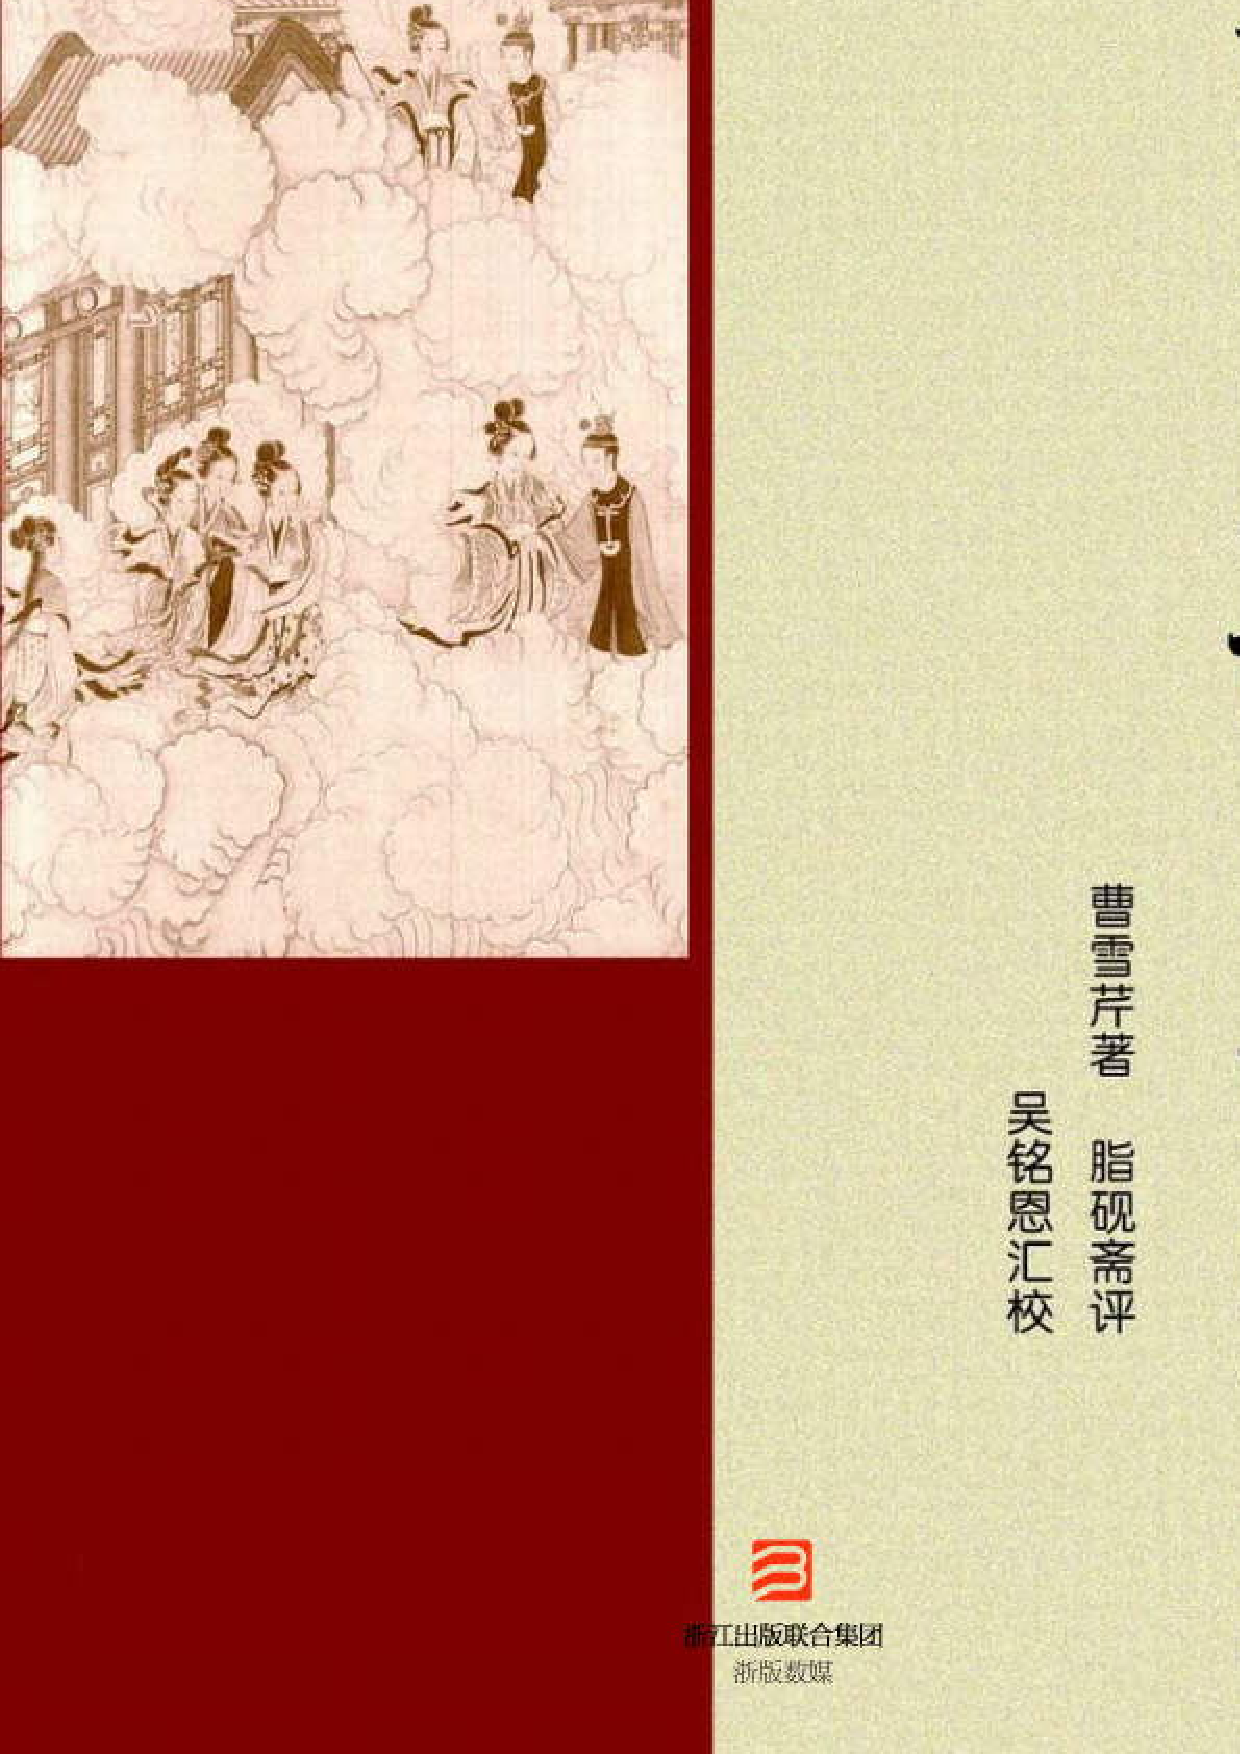
\includepdf{../Images/cover} 加上这张很糊的封面图反而不好看了。所以不加
	%\TileSquareWallPaper{1}{cover}这么用可以改变整个文档的背景
	\author{曹雪芹}
	\title{红楼梦脂评汇校本}
	\date{\today}
	\maketitle
	\frontmatter
	\chapter{版权信息}
\begin{flushleft}
	
{红楼梦脂评汇校本}\\
曹雪芹著~~脂砚斋评~~吴铭恩汇校\\[2\baselineskip]\copyright 浙江出版集团数字传媒有限公司~2016\\
本书版权为浙江出版集团数字传媒有限公司所有,未经书面授权,不得在任何地区以任何方式转载、翻印、仿制或节录本书文字或图片。

DNA-BN:ECFP-N00004139-20160531\\
最后修订:2016年5月31日\\
编辑\&amp;制作:{肖若臻}\\

tex文件源代码由epub经pandoc转出,
使用工具
\begin{itemize}
	\item Notepad++
	\item 排版助手
	\item Sigil
	\item Adobe Acrobat XI Pro
	\item TeXstudio
	\item Inkscape
\end{itemize}
离宫:1694892905@qq.com\\

出版:浙江出版集团数字传媒有限公司\\
浙江~杭州~体育场路347号\\
互联网出版许可证:新出网证(浙)字10号\\
电子邮箱:cb@bookdna.cn\\
网  址:www.bookdna.cn\\
BookDNA是浙江出版联合集团旗下电子书出版机构,为作者提供电子书出版服务。\\
如您发现本书内容错讹,敬请指正,以便新版修订。\\
吴铭恩:kolistan@vip.qq.com\\

\copyright Zhejiang Publishing United Group Digital Media CO.,LTD,2014\\
No.347 Tiyuchang Road, Hangzhou 310006 P.R.C.\\
cb@bookdna.cn\\
www.bookdna.cn

% \hypertarget{part0001_split_000.htmlux5cux23calibre_pb_0}{}

% \protect\hypertarget{part0001_split_001.html}{}{}

% \hypertarget{part0001_split_001.htmlux5cux23calibre_pb_1}{}
北方联合出版传媒集团 万卷出版公司 2013.10\\
ISBN:9787547028056
\end{flushleft}
\begin{center}
	\includegraphics[width=7cm]{../images/0001}
	\begin{center}
		{\LARGE 扫描二维码获取本书纸质版}
	\end{center}
\end{center}

	\chapter{整理说明}

《红楼梦脂评汇校本》,系以甲戌本、己卯本、庚辰本等早期脂本为底本,汇集了戚序本、蒙府本等其他脂批本的部分脂批,并参考、吸收若干新校点本及脂批辑本的校点成果整理而成。对前人意见有分歧的,略参己意而取舍,力求既不人云亦云,也不标新立异,整理成为一个方便阅读和检索的脂评红楼梦简明读本。

本书正文以甲戌本及庚辰本为底本(第六十四、六十七回以列藏本为底本),以其他各脂本参校。甲戌本所存十六回,文字显著优于他本,基本照录原文,只在确有必要时改动少量字词;庚辰本内容比较完整,惜抄写草率,错误甚多,不得不参照己卯本等本子校改大量字句。第六十七回两种版本文字差异过大,无法互校,一并附录。

本书辑录现存各脂本上的固有批语,并剔除在抄本流传过程中收藏者或读者所加的批语。批语按以下顺序辑录:甲戌本、己卯本、庚辰本、戚序本、蒙府本、列藏本、甲辰本。为节省篇幅,后出版本的批语与前面某本文字相同的,不再列出;有个别文字差异的,只据以参校,也不单独列出。

为节省篇幅,本书辑录批语使用略字,意义如下:\includegraphics[width=3mm]{../Images/00002}(甲戌本)、\includegraphics[width=3mm]{../Images/00003}(己卯本)、\includegraphics[width=3mm]{../Images/00004}(庚辰本)、\includegraphics[width=3mm]{../Images/00005}(戚序本)、\includegraphics[width=3mm]{../Images/00006}(蒙府本)、\includegraphics[width=3mm]{../Images/00007}(列藏本)、\includegraphics[width=3mm]{../Images/00008}(杨藏本)、\includegraphics[width=3mm]{../Images/00009}(甲辰本);\includegraphics[width=3mm]{../Images/00010} (眉批。原抄在页眉{[}正文上边{]}的批语)、\includegraphics[width=3mm]{../Images/00011} (侧批。原抄在正文右侧的批语)、\includegraphics[width=3mm]{../Images/00012}  (夹批。原抄在正文中间的双行批语)。为醒目起见,本书正文排为宋体字,批语排为楷体小号字:朱批仍用红色,墨批仍用黑色。抄本中有些同一位置不止一条批语的,原以``○''或空格隔开,现统一以``◇''隔开。

本书使用半角圆括号()和半角方括号{[}{]}作为校改文字记号:(某)表示删字,{[}某{]}表示补字,(甲){[}乙{]}表示改字。为避免校改记号过多影响阅读,对明显错字及前人意见比较一致的校改成果,径改而不标记。

本书曾以电子版的形式在网络上广泛流传,产生了一定的影响。在电子版整理过程中,抚琴居网站的朋友们浪知、君子九思、爱如潮水、娄员外、梁三、兔子她妈、休闲、志学斋主、daphne等协助覆校,订正不少错误;冰冰冰冷、云涛、yupeng、蓝山、潇湘楚客、zhwl、liuzhoufish、寻梦园、阿迦、影乐之声、rocwings等诸位先后指出了若干问题,统此鸣谢。在电子版传播过程中,许多朋友提出了出版纸版书的建议,还有一些朋友自行打印装订成册,以方便阅读使用。今天本书终得印行,要特别感谢上海《红楼梦研究辑刊》主编萧凤芝老师、白山出版社原总编董志新老师的大力支持和协助;感谢八一电影制片厂高级美工师汪德龙老师为本书题签。

由于整理者学识所限,本书虽经多次修订,存在问题必然尚多。希望朋友们在使用过程中发现错误及不妥之处,继续不吝赐教。

\begin{flushright}
	吴铭恩 ~2013.9.30.
\end{flushright}~~~~

	\chapter{脂砚斋重评石头记凡例}

{\kaishu {《红楼梦》旨义} 是书题名极{[}多,一曰《红楼]\kaishu 梦》,是总其全部之名也;又曰《风月宝鉴》,是戒妄动风月之情;又曰《石头记》,是自譬石头所记之事也。此三名皆书中曾已点睛矣。如宝玉作梦,梦中有曲,名曰《红楼梦十二支》,此则《红楼梦》之点睛。又如贾瑞病,跛道人持一镜来,上面即錾``风月宝鉴''四字,此则《风月宝鉴》之点睛。又如道人亲眼见石上大书一篇故事,则系石头所记之往来,此则《石头记》之点睛处。然此书又名曰《金陵十二钗》,审其名,则必系金陵十二女子也;然通部细搜检去,上中下女子岂止十二人哉!若云其中自有十二个,则又未尝指明白系某某,及至``红楼梦''一回中,亦曾翻出金陵十二钗之簿籍,又有十二支曲可考。}

{\kaishu 书中凡写长安,在文人笔墨之间,则从古之称;凡愚夫妇、儿女子家常口角,则曰``中京'',是不欲着迹于方向也。盖天子之邦,亦当以中为尊,特避其东南西北四字样也。}

{\kaishu 此书只是着意于闺中,故叙闺中之事切,略涉于外事者则简,不得谓其不均也。}

{\kaishu 此书不敢干涉朝廷,凡有不得不用朝政者,只略用一笔带出,盖实不敢以写儿女之笔墨唐突朝廷之上也,又不得谓其不备。}

{\kaishu 此书开卷第一回也,作者自云:因曾历过一番梦幻之后,故将真事隐去,而撰此《石头记》一书也。故曰``甄士隐梦幻识通灵''。但书中所记何事?又因何而撰是书哉?自云:今风尘碌碌,一事无成,忽念及当日所有之女子,一一细推了去,觉其行止见识皆出于我之上,何堂堂之须眉诚不若彼一干裙钗?实愧则有馀、悔则无益之大无可奈何之日也。当此时,则自欲将已往所赖------上赖天恩,下承祖德,锦衣纨袴之时,饫甘餍美之日,背父母教育之恩,负师兄规训之德,以致今日一事无成、半生潦倒之罪,编述一记,以告普天下人。虽我之罪固不能免,然闺阁中本自历历有人,万不可因我不肖,则一并使其泯灭也。虽今日之茅椽蓬牖,瓦灶绳床,其风晨月夕,阶柳庭花,亦未有伤于我之襟怀笔墨者。何为不用假语村言敷演出一段故事来,以悦人之耳目哉?故曰``{[}贾雨村{]}风尘怀闺秀'',乃是第一回题纲正义也。开卷即云``风尘怀闺秀'',则知作者本意原为记述当日闺友闺情,并非怨世骂时之书矣。虽一时有涉于世态,然亦不得不叙者,但非其本旨耳。阅者切记之。}

{\kaishu 诗曰:}

{\kaishu  浮生着甚苦奔忙,盛席华筵终散场。}

{\kaishu  悲喜千般同幻渺,古今一梦尽荒唐。}

{\kaishu  谩言红袖啼痕重,更有情痴抱恨长。}

{\kaishu  字字看来皆是血,十年辛苦不寻常。}

% {\href{../Text/part0004.html\#navto_1_a}{①}此凡例五条及题诗仅见于甲戌本卷首,退二格抄写。其他各本均无凡例,且均截取第五条``此开卷第一回也''并入第一回作为正文开始。}
% {\href{../Text/part0004.html\#navto_2_a}{②}此处原被撕去一角,缺五字。胡适补书``多''``红楼''三字,吴恩裕另校补``一曰''两字。除``红楼''二字无争议外,前三字所补是否恰当,有不同意见。}
	
    \mainmatter
\tableofcontents
\include{./TeX_files/chapter01}
\include{./TeX_files/chapter02}

%{{第三回}}{第三回}}

\chapter{金陵城起复贾雨村 荣国府收养\textsuperscript{*}林黛玉}

*{\includegraphics[width=3mm]{../Images/00002}\includegraphics[width=3mm]{../Images/00011}\footnotesize \kaishu 二字触目凄凉之至!}

{\includegraphics[width=3mm]{../Images/00005}\kaishu  我为你持戒,我为你吃斋;我为你百行百计不舒怀,我为你泪眼愁眉难解。无人处,自疑猜,生怕那慧性灵心偷改。}

{\kaishu 宝玉通灵可爱,天生有眼堪穿。万年幸一遇仙缘,从此春光美满。随时喜怒哀乐,远却离合悲欢。地久天长香影连,可意方舒心眼。}

{\kaishu 宝玉衔来,是补天之馀,落地已久,得地气收藏,因人而现。其性质内阳外阴,其形体光白温润,天生有眼可穿,故名曰宝玉,将欲得者尽皆宝爱此玉之意也。}

{\kaishu 天地循环秋复春,生生死死旧重新。君家着笔描风月,宝玉颦颦解爱人。}

却说雨村忙回头看时,不是别人,乃是当日同僚一案参革的号张如圭{\includegraphics[width=3mm]{../Images/00002}\includegraphics[width=3mm]{../Images/00011}\footnotesize \kaishu 盖言``如鬼如蜮''也,亦非正人正言。}者。他本系此地人,革职后家居,今打听得都中奏准起复旧员之信,他便四下里寻情找门路,忽遇见雨村,故忙道喜。{\includegraphics[width=3mm]{../Images/00006}\includegraphics[width=3mm]{../Images/00011}\footnotesize \kaishu {(此)}{[}仕{]}途宦境,描写的当。}二人见了礼,张如圭便将此信告诉雨村,雨村自是欢喜,忙忙的叙了两句,{\includegraphics[width=3mm]{../Images/00002}\includegraphics[width=3mm]{../Images/00011}\footnotesize \kaishu 画出心事。}遂作别各自回家。冷子兴听得此言,便忙献计,{\includegraphics[width=3mm]{../Images/00002}\includegraphics[width=3mm]{../Images/00011}\footnotesize \kaishu 毕肖赶热灶者。}令雨村央烦林如海,转向都中去央烦贾政。雨村领其意,作别回至馆中,忙寻邸报看真确了。{\includegraphics[width=3mm]{../Images/00002}\includegraphics[width=3mm]{../Images/00011}\footnotesize \kaishu 细!}

次日,面谋之如海。如海道:``天缘凑巧,因贱荆去世,都中家岳母念及小女无人依傍教育,前已遣了男女船只来接,因小女未曾大痊,故未及行。此刻正思向蒙训教之恩未经酬报,遇此机会,岂有不尽心图报之理。但请放心,弟已预为筹画至此,已修下荐书一封,转托内兄务为周全协佐,方可稍尽弟之鄙诚,即有所费用之例,弟于内兄信中已注明白,亦不劳尊兄多虑矣。''{\includegraphics[width=3mm]{../Images/00006}\includegraphics[width=3mm]{../Images/00011}\footnotesize \kaishu 要说正文故以此作引,且黛玉路中实无可托之人。文笔逼切得宜。}雨村一面打躬,谢不释口,一面又问:``不知令亲大人现居何职?{\includegraphics[width=3mm]{../Images/00002}\includegraphics[width=3mm]{../Images/00011}\footnotesize \kaishu 奸险小人欺人语。}只怕晚生草率,不敢骤然入都干渎。''{{\includegraphics[width=3mm]{../Images/00002}\includegraphics[width=3mm]{../Images/00011}\footnotesize \kaishu 全是假,全是诈。 }\includegraphics[width=3mm]{../Images/00006}\includegraphics[width=3mm]{../Images/00011}\footnotesize \kaishu 借雨村细密心思之语,容容易易转入正文,亦是宦途人之口头心头。最妙!}如海笑道:``若论舍亲,与尊兄犹系同谱,乃荣公之孙。大内兄现袭一等将军之职,名赦,字恩侯;二内兄名政,字存周,{\includegraphics[width=3mm]{../Images/00002}\includegraphics[width=3mm]{../Images/00011}\footnotesize \kaishu 二名二字皆颂德而来,与子兴口中作证。}现任工部员外郎,其为人谦恭厚道,大有祖父遗风,非膏粱轻薄仕宦之流,故弟方致书烦托。否则不但有污尊兄之清操,即弟亦不屑为矣。''{{\includegraphics[width=3mm]{../Images/00002}\includegraphics[width=3mm]{../Images/00011}\footnotesize \kaishu 写如海实写政老。所谓此书有``不写之写''是也。 }\includegraphics[width=3mm]{../Images/00006}\includegraphics[width=3mm]{../Images/00011}\footnotesize \kaishu 作弊者每每偏能如此说。}雨村听了,心下方信了昨日子兴之言,于是又谢了林如海。如海乃说:``已择了出月初二日小女入都,尊兄即同路而往,岂不两便?''雨村唯唯听命,心中十分得意。如海遂打点礼物并饯行之事,雨村一一领了。

那女学生黛玉,身体大愈,原不忍弃父而往,无奈他外祖母致意务去,且兼如海说:``汝父年将半百,再无续室之意,且汝多病,年又极小,上无亲母教养,下无姊妹兄弟扶持,{\includegraphics[width=3mm]{../Images/00002}\includegraphics[width=3mm]{../Images/00011}\footnotesize \kaishu 可怜!一句一滴血,一句一滴血之文。}今依傍外祖母及舅氏姊妹去,正好减我顾盼之忧,何云不往?''黛玉听了,方洒泪拜别,{{\includegraphics[width=3mm]{../Images/00002}\includegraphics[width=3mm]{../Images/00011}\footnotesize \kaishu 实写黛玉。 }\includegraphics[width=3mm]{../Images/00006}\includegraphics[width=3mm]{../Images/00011}\footnotesize \kaishu 此一段是不肯使黛玉作弃父乐为远游者。以此可见作者之心宝爱黛玉如己。}随同奶娘及荣府几个老妇人登舟而去。雨村另有一只船,带两个小童,依附黛玉而行。{{\includegraphics[width=3mm]{../Images/00002}\includegraphics[width=3mm]{../Images/00011}\footnotesize \kaishu 老师依附门生,怪道今时以收纳门生为幸。 }\includegraphics[width=3mm]{../Images/00006}\includegraphics[width=3mm]{../Images/00011}\footnotesize \kaishu 细密如此,是大家风范。}

有日到了都中,{\includegraphics[width=3mm]{../Images/00002}\includegraphics[width=3mm]{../Images/00011}\footnotesize \kaishu 繁中减笔。}进入神京,雨村先整了衣冠,{\includegraphics[width=3mm]{../Images/00002}\includegraphics[width=3mm]{../Images/00011}\footnotesize \kaishu 且按下黛玉以待细写。今故先将雨村安置过一边,方起荣府中之正文也。}带了小童,{\includegraphics[width=3mm]{../Images/00002}\includegraphics[width=3mm]{../Images/00011}\footnotesize \kaishu 至此渐渐好看起来也。}拿着宗侄的名帖,{\includegraphics[width=3mm]{../Images/00002}\includegraphics[width=3mm]{../Images/00011}\footnotesize \kaishu 此帖妙极,可知雨村的品行矣。}至荣府门前投了。彼时贾政已看了妹丈之书,即忙请入相会。见雨村相貌魁伟,言谈不俗,且这贾政最喜读书人,礼贤下士,拯溺济危,大有祖风,况又系妹丈致意,因此优待雨村,{\includegraphics[width=3mm]{../Images/00002}\includegraphics[width=3mm]{../Images/00011}\footnotesize \kaishu 君子可欺{[}以{]}其方也,况雨村正在王莽谦恭下士之时,虽政老亦为所惑,在作者系指东说西也。}更又不同,便竭力内中协助。题奏之日,轻轻谋{\includegraphics[width=3mm]{../Images/00002}\includegraphics[width=3mm]{../Images/00011}\footnotesize \kaishu 《春秋》字法。}了一个复职候缺,不上两个月,金陵应天府缺出,便谋补{\includegraphics[width=3mm]{../Images/00002}\includegraphics[width=3mm]{../Images/00011}\footnotesize \kaishu 《春秋》字法。}了此缺,拜辞了贾政,择日到任去了。{\includegraphics[width=3mm]{../Images/00002}\includegraphics[width=3mm]{../Images/00011}\footnotesize \kaishu 因宝钗故及之,一语过至下回。}不在话下。{\includegraphics[width=3mm]{../Images/00006}\includegraphics[width=3mm]{../Images/00011}\footnotesize \kaishu 了结雨村。}

且说黛玉自那日弃舟登岸时,{\includegraphics[width=3mm]{../Images/00002}\includegraphics[width=3mm]{../Images/00011}\footnotesize \kaishu 这方是正文起头处。此后笔墨,与前两回不同。}便有荣国府打发了轿子并拉行李的车辆久候了。这黛玉常听得{{\includegraphics[width=3mm]{../Images/00002}\includegraphics[width=3mm]{../Images/00011}\footnotesize \kaishu 三字细。 }\includegraphics[width=3mm]{../Images/00006}\includegraphics[width=3mm]{../Images/00011}\footnotesize \kaishu 以``常听见''等字,省下多少笔墨。}母亲说过,他外祖母家与别家不同。他近日所见的这几个三等的仆妇,已是不凡了,何况今至其家。因此步步留心,时时在意,不肯轻意多说一句话,多行一步路,{\includegraphics[width=3mm]{../Images/00006}\includegraphics[width=3mm]{../Images/00011}\footnotesize \kaishu 颦颦故自不凡。}生恐被人耻笑了他去。{{\includegraphics[width=3mm]{../Images/00002}\includegraphics[width=3mm]{../Images/00011}\footnotesize \kaishu 写黛玉自幼之心机。 }\includegraphics[width=3mm]{../Images/00009}\includegraphics[width=3mm]{../Images/00012}\footnotesize \kaishu 黛玉自忖之语。}自上了轿,进入城中,从纱窗向外瞧了一瞧,其街市之繁华,人烟之阜盛,自与别处不同。{\includegraphics[width=3mm]{../Images/00002}\includegraphics[width=3mm]{../Images/00011}\footnotesize \kaishu 先从街市写来。}又行了半日,忽见街北蹲着两个大石狮子,三间兽头大门,门前列坐着十来个华冠丽服之人。正门却不开,只有东西两角门有人出入。正门之上有一匾,匾上大书``敕造宁国府''五个大字。{\includegraphics[width=3mm]{../Images/00002}\includegraphics[width=3mm]{../Images/00011}\footnotesize \kaishu 先写宁府,这是由东向西而来。}黛玉想道:``这是外祖母之长房了。''想着,又往西行,不多远,照样也是三间大门,方是荣国府了。却不进正门,{\includegraphics[width=3mm]{../Images/00006}\includegraphics[width=3mm]{../Images/00011}\footnotesize \kaishu 以下写{(宁)}{[}荣{]}国府第,总借黛玉一双俊眼中传来。非黛玉之眼,也不得如此细密周详。}只进了西边角门。那轿夫抬进去,走了一射之地,将转弯时,便歇下退出去了。后面婆子们已都下了轿,赶上前来。另换了三四个衣帽周全的十七八岁的小厮上来,复抬起轿子。众婆子步下围随,至一垂花门前落下。众小厮退出,众婆子上来打起轿帘,扶黛玉下轿。{\includegraphics[width=3mm]{../Images/00006}\includegraphics[width=3mm]{../Images/00011}\footnotesize \kaishu 以上写款项。}林黛玉扶着婆子的手,进了垂花门,两边是抄手游廊,当中是穿堂,当地放着一个紫檀架子大理石的大插屏。转过插屏,小小三间内厅,厅后就是后面的正房大院。正面五间上房,皆是雕梁画栋,两边穿山游廊厢房,挂着各色鹦鹉、画眉等鸟雀。台矶之上,坐着几个穿红着绿的丫鬟,一见他们来了,便忙都笑迎上来,说:``才刚老太太还念呢,可巧就来了。''{\includegraphics[width=3mm]{../Images/00002}\includegraphics[width=3mm]{../Images/00011}\footnotesize \kaishu 如见如闻,活现于纸上之笔。好看煞!}于是三四人争着打起帘栊,{\includegraphics[width=3mm]{../Images/00002}\includegraphics[width=3mm]{../Images/00011}\footnotesize \kaishu 真有是事,真有是事!}一面听得人回话:``林姑娘到了。''

黛玉方进入房时,只见两个人搀着一位鬓发如银的老母迎上来,{\includegraphics[width=3mm]{../Images/00002}\includegraphics[width=3mm]{../Images/00010}\footnotesize \kaishu 此书得力处,全是此等地方,所谓``颊上三毫''也。}黛玉便知是他外祖母。方欲拜见时,早被他外祖母一把搂入怀中,``心肝儿肉''{\includegraphics[width=3mm]{../Images/00005}\includegraphics[width=3mm]{../Images/00012}\footnotesize \kaishu 写尽天下疼女儿的神理。 \includegraphics[width=3mm]{../Images/00006}\includegraphics[width=3mm]{../Images/00011}\footnotesize \kaishu 此一段文字是天性中流出,我读时不觉泪盈双袖。}叫着大哭起来。{\includegraphics[width=3mm]{../Images/00002}\includegraphics[width=3mm]{../Images/00011}\footnotesize \kaishu 几千斤力量写此一笔。}当下地下侍立之人,无不掩面涕泣,{\includegraphics[width=3mm]{../Images/00002}\includegraphics[width=3mm]{../Images/00011}\footnotesize \kaishu 旁写一笔,更妙!}黛玉也哭个不住。{{\includegraphics[width=3mm]{../Images/00002}\includegraphics[width=3mm]{../Images/00011}\footnotesize \kaishu 自然顺写一笔。 }\includegraphics[width=3mm]{../Images/00006}\includegraphics[width=3mm]{../Images/00011}\footnotesize \kaishu 逼真。}一时众人慢慢的解劝住了,黛玉方拜见了外祖母。{\includegraphics[width=3mm]{../Images/00002}\includegraphics[width=3mm]{../Images/00010}\footnotesize \kaishu 书中正文之人,却如此写出,却是天生地设章法,不见一丝勉强。}此即冷子兴所云之史氏太君,贾赦、贾政之母也。{\includegraphics[width=3mm]{../Images/00002}\includegraphics[width=3mm]{../Images/00011}\footnotesize \kaishu 书中人目太繁,故明注一笔,使观者省眼。}当下贾母一一指与黛玉:``这是你大舅母,{\includegraphics[width=3mm]{../Images/00009}\includegraphics[width=3mm]{../Images/00012}\footnotesize \kaishu 邢氏。}这是你二舅母,{\includegraphics[width=3mm]{../Images/00009}\includegraphics[width=3mm]{../Images/00012}\footnotesize \kaishu 王氏。}这是你先珠大哥的媳妇珠大嫂。{\includegraphics[width=3mm]{../Images/00009}\includegraphics[width=3mm]{../Images/00012}\footnotesize \kaishu 李纨。}''黛玉一一拜见过。贾母又说:``请姑娘们来。今日远客才来,可以不必上学去了。''众人答应了一声,便去了两个。

不一时,只见三个奶嬷嬷并五六个丫鬟,簇拥着三个姊妹来了。{\includegraphics[width=3mm]{../Images/00002}\includegraphics[width=3mm]{../Images/00011}\footnotesize \kaishu 声势如现纸上。 \includegraphics[width=3mm]{../Images/00002}\includegraphics[width=3mm]{../Images/00010}\footnotesize \kaishu 从黛玉眼中写三人。}第一个肌肤微丰,{\includegraphics[width=3mm]{../Images/00002}\includegraphics[width=3mm]{../Images/00011}\footnotesize \kaishu 不犯宝钗。}合中身材,腮凝新荔,鼻腻鹅脂,温柔沉默,观之可亲。{\includegraphics[width=3mm]{../Images/00002}\includegraphics[width=3mm]{../Images/00011}\footnotesize \kaishu 为迎春写照。}第二个削肩细腰,{\includegraphics[width=3mm]{../Images/00002}\includegraphics[width=3mm]{../Images/00011}\footnotesize \kaishu 《洛神赋》中云``肩若削成''是也。}长挑身材,鸭蛋脸面,俊眼修眉,顾盼神飞,文彩精华,见之忘俗。{\includegraphics[width=3mm]{../Images/00002}\includegraphics[width=3mm]{../Images/00011}\footnotesize \kaishu 为探春写照。}第三个身量未足,形容尚小。{\includegraphics[width=3mm]{../Images/00002}\includegraphics[width=3mm]{../Images/00010}\footnotesize \kaishu 浑写一笔更妙!必个个写去则板矣。可笑近之小说中有一百个女子,皆是如花似玉一副脸面。}其钗环裙袄,{\includegraphics[width=3mm]{../Images/00002}\includegraphics[width=3mm]{../Images/00011}\footnotesize \kaishu 是极。}三人皆是一样的妆饰。{{\includegraphics[width=3mm]{../Images/00002}\includegraphics[width=3mm]{../Images/00011}\footnotesize \kaishu 毕肖。 }\includegraphics[width=3mm]{../Images/00006}\includegraphics[width=3mm]{../Images/00011}\footnotesize \kaishu 欲画天尊,先画{(纵)}{[}众{]}神。如此,其天尊自当另有一番高山世外的景象。}黛玉忙起身迎上来见礼,{\includegraphics[width=3mm]{../Images/00002}\includegraphics[width=3mm]{../Images/00011}\footnotesize \kaishu 此笔亦不可少。}互相厮认过,大家归坐。丫鬟们斟上茶来。不过说些黛玉之母如何得病,如何请医服药,如何送死发丧。不免贾母又伤感起来,{{\includegraphics[width=3mm]{../Images/00002}\includegraphics[width=3mm]{../Images/00011}\footnotesize \kaishu 妙! }\includegraphics[width=3mm]{../Images/00006}\includegraphics[width=3mm]{../Images/00011}\footnotesize \kaishu 层层不露,周密之至。}因说:``我这些儿女,所疼者惟有你母,今日一旦先舍我去了,连面也不能一见,今见了你,我怎么不伤心!''说着,搂了黛玉在怀,又呜咽起来。{\includegraphics[width=3mm]{../Images/00006}\includegraphics[width=3mm]{../Images/00011}\footnotesize \kaishu 不禁我也跟他哭起。}众人忙都宽慰解释,方略略止住。{\includegraphics[width=3mm]{../Images/00002}\includegraphics[width=3mm]{../Images/00011}\footnotesize \kaishu 总为黛玉自此不能别往。}

众人见黛玉年貌虽小,其举止言谈不俗,身体面庞虽怯弱不胜,{\includegraphics[width=3mm]{../Images/00002}\includegraphics[width=3mm]{../Images/00011}\footnotesize \kaishu 写美人是如此笔仗,看官怎得不叫绝称赏!}却有一段自然风流态度,{\includegraphics[width=3mm]{../Images/00002}\includegraphics[width=3mm]{../Images/00011}\footnotesize \kaishu 为黛玉写照。众人目中,只此一句足矣。 \includegraphics[width=3mm]{../Images/00002}\includegraphics[width=3mm]{../Images/00010}\footnotesize \kaishu 从众人目中写黛玉。◇草胎卉质,岂能胜物耶?想其衣裙皆不得不勉强支持者也。}便知他有不足之症。因问:``常服何药,如何不急为疗治?''黛玉笑道:``我自来是如此,从会吃饮食时便吃药,到今未断,请了多少名医修方配药,皆不见效。那一年我才三岁时,听得说{\includegraphics[width=3mm]{../Images/00002}\includegraphics[width=3mm]{../Images/00011}\footnotesize \kaishu 文字细如牛毛。}来了一个癞头和尚,{\includegraphics[width=3mm]{../Images/00002}\includegraphics[width=3mm]{../Images/00010}\footnotesize \kaishu 奇奇怪怪一至于此。通部中假借癞僧、跛道二人点明迷情幻海中有数之人也。非袭《西游》中一味无稽、至不能处便用观世音可比。}说要化我去出家,我父母固是不从。他又说:`既舍不得他,只怕他的病一生也不能好的了。若要好时,除非从此以后总不许见哭声,{\includegraphics[width=3mm]{../Images/00005}\includegraphics[width=3mm]{../Images/00012}\footnotesize \kaishu 爱哭的偏写出有人不教哭。 \includegraphics[width=3mm]{../Images/00006}\includegraphics[width=3mm]{../Images/00011}\footnotesize \kaishu 作者既以黛玉为绛珠化生,是要哭的了,反要使人先叫他不许哭。妙!}除父母之外,凡有外姓亲友之人,一概不见,方可平安了此一世。'疯疯癫癫,说了这些不经之谈,{\includegraphics[width=3mm]{../Images/00002}\includegraphics[width=3mm]{../Images/00011}\footnotesize \kaishu 是作书者自注。}也没人理他。如今还是吃人参养荣丸。''{\includegraphics[width=3mm]{../Images/00002}\includegraphics[width=3mm]{../Images/00011}\footnotesize \kaishu 人生自当自养荣卫。 \includegraphics[width=3mm]{../Images/00002}\includegraphics[width=3mm]{../Images/00010}\footnotesize \kaishu 甄英莲乃副十二钗之首,却明写癞僧一点。今黛玉为正十二钗之冠,反用暗笔。盖正十二钗人或洞悉可知,副十二钗或恐观者忽略,故写极力一提,使观者万勿稍加玩忽之意耳。}贾母道:``这正好,我这里正配丸药呢。叫他们多配一料就是了。''{\includegraphics[width=3mm]{../Images/00002}\includegraphics[width=3mm]{../Images/00011}\footnotesize \kaishu 为后菖、菱伏脉。}

一语未了,只听得后院中有人笑声{\includegraphics[width=3mm]{../Images/00002}\includegraphics[width=3mm]{../Images/00011}\footnotesize \kaishu 懦笔庸笔何能及此!}说:``我来迟了,不曾迎接远客!''{{\includegraphics[width=3mm]{../Images/00002}\includegraphics[width=3mm]{../Images/00011}\footnotesize \kaishu 第一笔,阿凤三魂六魄已被作者拘定了,后文焉得不活跳纸上?此等文字非仙助{(即)}{[}亦{]}非神助,从何而得此机括耶? \includegraphics[width=3mm]{../Images/00002}\includegraphics[width=3mm]{../Images/00010}\footnotesize \kaishu 另磨新墨,搦锐笔,特独出熙凤一人。未写其形,先使闻声,所谓``绣幡开,遥见英雄俺''也。}}黛玉纳罕道:``这些人个个皆敛声屏气,恭肃严整如此,这来者系谁,这样放诞无礼?''{{\includegraphics[width=3mm]{../Images/00002}\includegraphics[width=3mm]{../Images/00011}\footnotesize \kaishu 原有此一想。 }\includegraphics[width=3mm]{../Images/00006}\includegraphics[width=3mm]{../Images/00011}\footnotesize \kaishu 天下事不可一概而论。}心下想时,只见一群媳妇丫鬟围拥着一个人从后房门进来。这个人打扮与众姑娘不同,彩绣辉煌,恍若神妃仙子:头上戴着金丝八宝攒珠髻,绾着朝阳五凤挂珠钗,{\includegraphics[width=3mm]{../Images/00002}\includegraphics[width=3mm]{../Images/00011}\footnotesize \kaishu 头。}项上带着赤金盘螭璎珞圈,{\includegraphics[width=3mm]{../Images/00002}\includegraphics[width=3mm]{../Images/00011}\footnotesize \kaishu 颈。}裙边系着豆绿宫绦、双衡比目玫瑰佩,{\includegraphics[width=3mm]{../Images/00002}\includegraphics[width=3mm]{../Images/00011}\footnotesize \kaishu 腰。}身上穿着缕金百蝶穿花大红洋缎窄褃袄,{\includegraphics[width=3mm]{../Images/00006}\includegraphics[width=3mm]{../Images/00011}\footnotesize \kaishu 大凡能事者,多是尚奇好异,不肯泛泛同流。}外罩五彩刻丝石青银鼠褂,下着翡翠撒花洋绉裙。一双丹凤三角眼,两弯柳叶吊梢眉,{\includegraphics[width=3mm]{../Images/00006}\includegraphics[width=3mm]{../Images/00011}\footnotesize \kaishu 非如此眼,非如此眉,不得为熙凤。作者读过《麻衣相法》。}身量苗条,体格风骚,粉面含春威不露,丹唇未启笑先闻。{{\includegraphics[width=3mm]{../Images/00002}\includegraphics[width=3mm]{../Images/00011}\footnotesize \kaishu 为阿凤写照。 \includegraphics[width=3mm]{../Images/00002}\includegraphics[width=3mm]{../Images/00010}\footnotesize \kaishu 试问诸公:从来小说中可有写形追像至此者? }\includegraphics[width=3mm]{../Images/00006}\includegraphics[width=3mm]{../Images/00011}\footnotesize \kaishu 英豪本等。}黛玉连忙起身接见。贾母笑{\includegraphics[width=3mm]{../Images/00002}\includegraphics[width=3mm]{../Images/00011}\footnotesize \kaishu 阿凤一至,贾母方笑,与后文多少``笑''字作偶。}道:``你不认得他,他是我们这里有名的一个泼皮破落户儿,南省俗谓作`辣子',你只叫他`凤辣子'就是。''{\includegraphics[width=3mm]{../Images/00002}\includegraphics[width=3mm]{../Images/00011}\footnotesize \kaishu 阿凤笑声进来,老太君打诨,虽是空口传声,却是补出一向晨昏起居,阿凤于太君处承欢应候一刻不可少之人,看官勿以闲文淡文也。}黛玉正不知以何称呼,{\includegraphics[width=3mm]{../Images/00006}\includegraphics[width=3mm]{../Images/00011}\footnotesize \kaishu 想黛玉此时神情,含浑可爱。}只见众姊妹都忙告诉他道:``这是琏嫂子。''黛玉虽不识,亦曾听见母亲说过,大舅贾赦之子贾琏,娶的就是二舅母王氏之内侄女,自幼假充男儿教养的,学名叫王熙凤。{\includegraphics[width=3mm]{../Images/00002}\includegraphics[width=3mm]{../Images/00011}\footnotesize \kaishu 奇想奇文。以女子曰``学名''固奇,然此偏有学名的反倒不识字,不曰学名者反若假。}黛玉忙陪笑见礼,以``嫂''呼之。这熙凤携着黛玉的手,上下细细的打量了一回,{\includegraphics[width=3mm]{../Images/00002}\includegraphics[width=3mm]{../Images/00011}\footnotesize \kaishu 写阿凤全部传神第一笔也。}便仍送至贾母身边坐下,因笑道:``天下真有这样标致人物,我今儿才算见了!{\includegraphics[width=3mm]{../Images/00002}\includegraphics[width=3mm]{../Images/00011}\footnotesize \kaishu 这方是阿凤言语。若一味浮词套语,岂复为阿凤哉! \includegraphics[width=3mm]{../Images/00002}\includegraphics[width=3mm]{../Images/00010}\footnotesize \kaishu ``真有这样标致人物''出自凤口,黛玉丰姿可知。宜作史笔看。}况且这通身的气派,竟不像老祖宗的外孙女儿,竟是个嫡亲的孙女,{\includegraphics[width=3mm]{../Images/00002}\includegraphics[width=3mm]{../Images/00011}\footnotesize \kaishu 仍归太君,方不失《石头记》文字,且是阿凤身心之至文。}怨不得老祖宗天天口头心头,一时不忘。{{\includegraphics[width=3mm]{../Images/00002}\includegraphics[width=3mm]{../Images/00011}\footnotesize \kaishu 却是极淡之语,偏能恰投贾母之意。 }\includegraphics[width=3mm]{../Images/00006}\includegraphics[width=3mm]{../Images/00011}\footnotesize \kaishu 以``真有''``怨不得''五字,写熙凤之口头,真是机巧异常,``怨不得''三字,愚弄了多少聪明特达者。}只可怜我这妹妹这样命苦,{\includegraphics[width=3mm]{../Images/00002}\includegraphics[width=3mm]{../Images/00011}\footnotesize \kaishu 这是阿凤见黛玉正文。}怎么姑妈偏就去世了!''{\includegraphics[width=3mm]{../Images/00002}\includegraphics[width=3mm]{../Images/00011}\footnotesize \kaishu 若无这几句,便不是贾府媳妇。}说着,便用帕拭泪。贾母笑道:``我才好了,你倒来招我。{\includegraphics[width=3mm]{../Images/00002}\includegraphics[width=3mm]{../Images/00011}\footnotesize \kaishu 文字好看之极。}你妹妹远路才来,身子又弱,也才劝住了,快再休提前话!''{\includegraphics[width=3mm]{../Images/00002}\includegraphics[width=3mm]{../Images/00011}\footnotesize \kaishu 反用贾母劝,看阿凤之术亦甚矣。}这熙凤听了,忙转悲为喜道:``正是呢!我一见了妹妹,一心都在他身上了,又是欢喜,又是伤心,竟忘记了老祖宗。该打,该打!''又忙携黛玉之手,问:``妹妹几岁了?可也上过学?现吃什么药?在这里不要想家,想要什么吃的、什么顽的,只管告诉我,丫头老婆们不好了,也只管告诉我。''一面又问婆子们:``林姑娘的行李东西可搬进来了?带了几个人来?{{\includegraphics[width=3mm]{../Images/00002}\includegraphics[width=3mm]{../Images/00011}\footnotesize \kaishu 当家的人本如此,毕肖! }\includegraphics[width=3mm]{../Images/00006}\includegraphics[width=3mm]{../Images/00011}\footnotesize \kaishu 三句话不离本行,职任在兹也。}你们赶早打扫两间下房,让他们去歇歇。''

说话时,已摆了茶果上来,熙凤亲为捧茶捧果。{{\includegraphics[width=3mm]{../Images/00002}\includegraphics[width=3mm]{../Images/00011}\footnotesize \kaishu 总为黛玉眼中写出。 }\includegraphics[width=3mm]{../Images/00006}\includegraphics[width=3mm]{../Images/00011}\footnotesize \kaishu 熙凤后到,为有事,写其劳能,先为筹画,写其机巧。摇前映后之笔。}又见二舅母问他:``月钱放完了不曾?''{\includegraphics[width=3mm]{../Images/00002}\includegraphics[width=3mm]{../Images/00011}\footnotesize \kaishu 不见后文,不见此笔之妙。}熙凤道:``月钱已放完了。才刚带着人到后楼上找缎子,{\includegraphics[width=3mm]{../Images/00002}\includegraphics[width=3mm]{../Images/00011}\footnotesize \kaishu 接闲文,是本意避繁也。}找了这半日,也并没有见昨日太太说的那样,{\includegraphics[width=3mm]{../Images/00002}\includegraphics[width=3mm]{../Images/00011}\footnotesize \kaishu 却是日用家常实事。}想是太太记错了?''{\includegraphics[width=3mm]{../Images/00006}\includegraphics[width=3mm]{../Images/00011}\footnotesize \kaishu 陪笔。用得灵活,兼能形容熙凤之为人。妙心妙手,故有妙文妙口。}王夫人道:``有没有,什么要紧。''因又说道:``该随手拿出两个来,给你这妹妹去裁衣裳的,{\includegraphics[width=3mm]{../Images/00002}\includegraphics[width=3mm]{../Images/00011}\footnotesize \kaishu 仍归前文。妙妙!}等晚上想着叫人再去拿罢,可别忘了。''熙凤道:``倒是我先料着了,知道妹妹不过这两日到的,我已预备下了,{\includegraphics[width=3mm]{../Images/00002}\includegraphics[width=3mm]{../Images/00010}\footnotesize \kaishu 余知此缎阿凤并未拿出,此借王夫人之语机变欺人处耳。若信彼果拿出预备,不独被阿凤瞒过,亦且被石头瞒过了。}等太太回去过了目好送来。''{\includegraphics[width=3mm]{../Images/00002}\includegraphics[width=3mm]{../Images/00011}\footnotesize \kaishu 试看他心机。}王夫人一笑,点头不语。{{\includegraphics[width=3mm]{../Images/00002}\includegraphics[width=3mm]{../Images/00011}\footnotesize \kaishu 深取之意。 }\includegraphics[width=3mm]{../Images/00009}\includegraphics[width=3mm]{../Images/00012}\footnotesize \kaishu 很漏凤姐是个当家人。}

当下茶果已撤,贾母命两个老嬷嬷带了黛玉去见两个母舅。时贾赦之妻邢氏忙亦起身,笑道:``我带了外甥女过去,倒也便宜。''{\includegraphics[width=3mm]{../Images/00006}\includegraphics[width=3mm]{../Images/00011}\footnotesize \kaishu 以黛玉之来去候安之便,便将荣宁二府的势排描写尽矣。}贾母笑道:``正是呢,你也去罢,不必过来了。''邢夫人答应一个``是''字,遂带了黛玉与王夫人作辞,大家送至穿堂前。出了垂花门,早有众小厮们拉过一辆翠幄青紬车来。邢夫人携了黛玉坐上,{\includegraphics[width=3mm]{../Images/00009}\includegraphics[width=3mm]{../Images/00012}\footnotesize \kaishu 未识黛卿能乘此否。}众婆子们放下车帘,方命小厮们抬起,拉至宽处,方驾上驯骡,亦出了西角门,往东过了荣府正门,便入一黑油大门中,至仪门前方下来。众小厮退出,方打起车帘,邢夫人搀了黛玉的手,进入院中。黛玉度其房屋院宇,必是荣府中之花园隔断过来的。{\includegraphics[width=3mm]{../Images/00002}\includegraphics[width=3mm]{../Images/00011}\footnotesize \kaishu 黛玉之心机眼力。}进入三层仪门,果见正房厢庑游廊,悉皆小巧别致,{\includegraphics[width=3mm]{../Images/00006}\includegraphics[width=3mm]{../Images/00011}\footnotesize \kaishu 分别得历历,可想如见。}不似方才那边轩峻壮丽,且院中随处之树木山石皆有。{\includegraphics[width=3mm]{../Images/00002}\includegraphics[width=3mm]{../Images/00011}\footnotesize \kaishu 为大观园伏脉。试思荣府园今在西,后之大观园偏写在东,何不畏难之若此?}一时进入正室,早有许多盛妆丽服之姬妾丫鬟迎着。邢夫人让黛玉坐了,一面命人到外面书房去请贾赦。{\includegraphics[width=3mm]{../Images/00002}\includegraphics[width=3mm]{../Images/00011}\footnotesize \kaishu 这一句都是写贾赦,妙在全是指东击西,打草惊蛇之笔。若看其写一人即作此一人看,先生便呆了。}一时人来回说:``老爷说了:`连日身上不好,见了姑娘彼此倒伤心,{\includegraphics[width=3mm]{../Images/00002}\includegraphics[width=3mm]{../Images/00011}\footnotesize \kaishu 追魂摄魄。 \includegraphics[width=3mm]{../Images/00002}\includegraphics[width=3mm]{../Images/00010}\footnotesize \kaishu 余久不作此语矣,见此语未免一醒。}暂且不忍相见。{{\includegraphics[width=3mm]{../Images/00002}\includegraphics[width=3mm]{../Images/00011}\footnotesize \kaishu 若一见时,不独死板,且亦大失情理,亦不能有此等妙文矣。 }\includegraphics[width=3mm]{../Images/00006}\includegraphics[width=3mm]{../Images/00011}\footnotesize \kaishu 作者绣口锦心,见有见的亲切,不见有不见的亲切,直说横讲,一毫不爽。}劝姑娘不要伤心想家,{\includegraphics[width=3mm]{../Images/00006}\includegraphics[width=3mm]{../Images/00011}\footnotesize \kaishu 亦在情理之内。}跟着老太太和舅母,即同家里一样。姊妹们虽拙,大家一处伴着,亦可以解些烦闷。{\includegraphics[width=3mm]{../Images/00002}\includegraphics[width=3mm]{../Images/00011}\footnotesize \kaishu 赦老亦能作此语,叹叹!}或有委屈之处,只管说得,不要外道才是。'''黛玉忙站起来,一一听了。再坐一刻,便告辞。那邢夫人苦留吃过晚饭去,黛玉笑回道:``舅母爱惜赐饭,原不应辞,只是还要过去拜见二舅舅,恐领了赐去不恭,{{\includegraphics[width=3mm]{../Images/00002}\includegraphics[width=3mm]{../Images/00011}\footnotesize \kaishu 得体。 }\includegraphics[width=3mm]{../Images/00006}\includegraphics[width=3mm]{../Images/00011}\footnotesize \kaishu 黛玉之为人,必当有如此身分。}异日再领,未为不可。望舅母容谅。''邢夫人听说,笑道:``这倒是了。''遂命两三个嬷嬷,用方才的车好生送了过去,于是黛玉告辞。邢夫人送至仪门前,又嘱咐众人几句,{\includegraphics[width=3mm]{../Images/00006}\includegraphics[width=3mm]{../Images/00011}\footnotesize \kaishu 又嘱咐了几句,方是舅母的本等。}眼看着车去了方回来。

一时黛玉进入荣府,下了车。众嬷嬷引着,便往东转弯,穿过一个东西的穿堂,{\includegraphics[width=3mm]{../Images/00002}\includegraphics[width=3mm]{../Images/00011}\footnotesize \kaishu 这一个穿堂是贾母正房之南者,凤姐处所通者则是贾母正房之北。}向南大厅之后,仪门内大院落,上面五间大正房,两边厢房鹿顶耳房钻山,四通八达,轩昂壮丽,比贾母处不同。黛玉便知这方是正经正内室,一条大甬路,直接出大门的。进入堂屋中,抬头迎面先看见一个赤金九龙青地大匾,匾上写着斗大三个字,是``荣禧堂'',{\includegraphics[width=3mm]{../Images/00006}\includegraphics[width=3mm]{../Images/00011}\footnotesize \kaishu 真是荣国府。}后有一行小字:``某年月日,书赐荣国公贾源。''又有``万几宸翰之宝''。大紫檀雕螭案上,设着三尺来高青绿古铜鼎,悬着待漏随朝墨龙大画,一边是金蜼彝,{\includegraphics[width=3mm]{../Images/00002}\includegraphics[width=3mm]{../Images/00011}\footnotesize \kaishu 蜼,音垒。周器也。}一边是玻璃\includegraphics[width=4mm]{../Images/00013}。{{{\includegraphics[width=3mm]{../Images/00002}\includegraphics[width=3mm]{../Images/00011}\footnotesize \kaishu }{\includegraphics[width=3mm]{../Images/00014},音海。盛酒之大器也。}}}地下两溜十六张楠木交椅。又有一副对联,乃是乌木联牌,镶着錾银的字迹,{\includegraphics[width=3mm]{../Images/00002}\includegraphics[width=3mm]{../Images/00011}\footnotesize \kaishu 雅而丽,富而文。}道是:

座上珠玑昭日月,堂前黼黻焕烟霞。{\includegraphics[width=3mm]{../Images/00002}\includegraphics[width=3mm]{../Images/00012}\footnotesize \kaishu 实贴。}

下面一行小字,道是:同乡世教弟勋袭东安郡王穆莳拜手书。{\includegraphics[width=3mm]{../Images/00002}\includegraphics[width=3mm]{../Images/00011}\footnotesize \kaishu 先虚陪一笔。}

原来王夫人时常居坐宴息,亦不在这正室,{\includegraphics[width=3mm]{../Images/00002}\includegraphics[width=3mm]{../Images/00011}\footnotesize \kaishu 黛玉由正室一段而来,是为拜见政老耳,故进东房。}只在这正室东边的三间耳房内。{\includegraphics[width=3mm]{../Images/00002}\includegraphics[width=3mm]{../Images/00011}\footnotesize \kaishu 若见王夫人,直写引至东廊小正室内矣。}于是老嬷嬷引黛玉进东房门来。临窗大炕上铺着猩红洋罽,正面设着大红金钱蟒靠背,石青金钱蟒引枕,秋香色金钱蟒大条褥。两边设一对梅花式洋漆小几。左边几上文王鼎、匙箸、香盒,右边几上汝窑美人觚------内插着时鲜花卉,并茗碗、唾壶等物。地下面西一溜四张椅上,都搭着银红撒花椅搭,底下四副脚踏。椅子两边,也有一对高几,几上茗碗花瓶俱备。其馀陈设,自不必细说。{\includegraphics[width=3mm]{../Images/00002}\includegraphics[width=3mm]{../Images/00011}\footnotesize \kaishu 此不过略叙荣府家常之礼数,特使黛玉一识阶级座次耳,馀则繁。}老嬷嬷们让黛玉炕上坐,炕沿上却也有两个锦褥对设,黛玉度其位次,便不上炕,只向东边椅子上坐了。{\includegraphics[width=3mm]{../Images/00002}\includegraphics[width=3mm]{../Images/00011}\footnotesize \kaishu 写黛玉心意。}本房内的丫鬟忙捧上茶来。黛玉一面吃茶,一面打量这些丫鬟们,{\includegraphics[width=3mm]{../Images/00006}\includegraphics[width=3mm]{../Images/00011}\footnotesize \kaishu 借黛玉眼写三等使婢。}妆饰衣裙,举止行动,果亦与别家不同。

茶未吃了,只见一个穿红绫袄、青缎掐牙背心的丫鬟{\includegraphics[width=3mm]{../Images/00002}\includegraphics[width=3mm]{../Images/00011}\footnotesize \kaishu 金乎?玉乎?}走来笑说道:``太太说,请姑娘到那边坐罢。''{\includegraphics[width=3mm]{../Images/00006}\includegraphics[width=3mm]{../Images/00011}\footnotesize \kaishu 唤去见,方是舅母,方是大家风范。}老嬷嬷听了,于是又引黛玉出来,到了东廊三间小正房内。正面炕上横设一张炕桌,桌上磊着书籍茶具,{\includegraphics[width=3mm]{../Images/00002}\includegraphics[width=3mm]{../Images/00011}\footnotesize \kaishu 伤心笔,堕泪笔。}靠东壁面西设着半旧青缎靠背引枕。王夫人却坐在西边下首,亦是半旧青缎靠背坐褥。见黛玉来了,便往东让。黛玉心中料定这是贾政之位。{\includegraphics[width=3mm]{../Images/00002}\includegraphics[width=3mm]{../Images/00011}\footnotesize \kaishu 写黛玉心到眼到,伧夫但云为贾府叙坐位,岂不可笑?}因见挨炕一溜三张椅子上,也搭着半旧的{\includegraphics[width=3mm]{../Images/00002}\includegraphics[width=3mm]{../Images/00011}\footnotesize \kaishu 三字有神。}弹墨椅袱,{\includegraphics[width=3mm]{../Images/00002}\includegraphics[width=3mm]{../Images/00011}\footnotesize \kaishu 此处则一色旧的,可知前正室中亦非家常之用度也。可笑近之小说中,不论何处,则曰商彝周鼎、绣幕珠帘、孔雀屏、芙蓉褥等样字眼。}黛玉便向椅上坐了。{\includegraphics[width=3mm]{../Images/00002}\includegraphics[width=3mm]{../Images/00010}\footnotesize \kaishu 近闻一俗笑语云:一庄农人进京回家,众人问曰:``你进京去可见些个世面否?''庄人曰:``连皇帝老爷都见了。''众罕然问曰:``皇帝如何景况?''庄人曰:``皇帝左手拿一金元宝,右手拿一银元宝,马上捎着一口袋人参,行动人参不离口。一时要屙屎了,连擦屁股都用的是鹅黄缎子,所以京中掏茅厕的人都富贵无比。''试思凡稗官写富贵字眼者,悉皆庄农进京之一流也。盖此时彼实未身经目睹,所言皆在情理之外焉。◇又如人嘲作诗者亦往往爱说富丽话,故有``胫骨变成金玳瑁,眼睛嵌作碧琉璃''之诮。余自是评《石头记》,非鄙薄前人也。}王夫人再四携他上炕,他方挨王夫人坐了。王夫人因说:``你舅舅今日斋戒去了,{\includegraphics[width=3mm]{../Images/00002}\includegraphics[width=3mm]{../Images/00011}\footnotesize \kaishu 点缀宦途。}再见罢。{\includegraphics[width=3mm]{../Images/00002}\includegraphics[width=3mm]{../Images/00011}\footnotesize \kaishu 赦老不见,又写政老。政老又不能见,是重不见重,犯不见犯。作者惯用此等章法。}只是有一句话嘱咐你:你三个姊妹倒都极好,以后一处念书认字学针线,或是偶一顽笑,都有尽让的。但我不放心的最是一件:{\includegraphics[width=3mm]{../Images/00006}\includegraphics[width=3mm]{../Images/00011}\footnotesize \kaishu 王夫人嘱咐与邢夫人嘱咐,似同{(的)}{[}而{]}迥异。儿女累心,我欲代伊哭诉一面愁苦。}我有一个孽根祸胎,{\includegraphics[width=3mm]{../Images/00002}\includegraphics[width=3mm]{../Images/00011}\footnotesize \kaishu 四字是血泪盈面,不得已无奈何而下。四字是作者痛哭。}是这家里的`混世魔王',{\includegraphics[width=3mm]{../Images/00002}\includegraphics[width=3mm]{../Images/00011}\footnotesize \kaishu 与``绛洞花王''为对看。}今日因庙里还愿去了,{\includegraphics[width=3mm]{../Images/00002}\includegraphics[width=3mm]{../Images/00011}\footnotesize \kaishu 是富贵公子。}尚未回来,晚间你看见便知。你只以后不要睬他,你这些姊妹都不敢沾惹他的。''

黛玉亦常听得母亲说过,二舅母生的有个表兄,乃衔玉而诞,顽劣异常,{\includegraphics[width=3mm]{../Images/00002}\includegraphics[width=3mm]{../Images/00011}\footnotesize \kaishu 与甄家子恰对。}极恶读书,{\includegraphics[width=3mm]{../Images/00002}\includegraphics[width=3mm]{../Images/00011}\footnotesize \kaishu 是极恶每日``诗云''``子曰''的读书。}最喜在内帏厮混,外祖母又极溺爱,无人敢管。今见王夫人如此说,便知说的是这表兄了。{\includegraphics[width=3mm]{../Images/00002}\includegraphics[width=3mm]{../Images/00010}\footnotesize \kaishu 这是一段反衬章法。黛玉心用``猜度蠢物''等句对着去,方不失作者本旨。}因陪笑道:``舅母说的,可是衔玉所生的这位哥哥?在家时亦曾听见母亲常说,{\includegraphics[width=3mm]{../Images/00006}\includegraphics[width=3mm]{../Images/00011}\footnotesize \kaishu 有曾听得,所以闻言便知,不必用心搜求了。}这位哥哥比我大一岁,小名就唤宝玉,{\includegraphics[width=3mm]{../Images/00002}\includegraphics[width=3mm]{../Images/00011}\footnotesize \kaishu 以黛玉道宝玉名,方不失正文。}虽{\includegraphics[width=3mm]{../Images/00002}\includegraphics[width=3mm]{../Images/00011}\footnotesize \kaishu ``虽''字是有情字,宿根而发,勿得泛泛看过。}极憨顽,说在姊妹情中极好的。{\includegraphics[width=3mm]{../Images/00006}\includegraphics[width=3mm]{../Images/00011}\footnotesize \kaishu 黛玉口中心中早中此。}况我来了,自然只和姊妹同处,兄弟们自是别院另室的,{\includegraphics[width=3mm]{../Images/00002}\includegraphics[width=3mm]{../Images/00011}\footnotesize \kaishu 又登开一笔,妙妙!}岂得去沾惹之理?''{\includegraphics[width=3mm]{../Images/00006}\includegraphics[width=3mm]{../Images/00011}\footnotesize \kaishu 用黛玉反衬一句,更有深味。}王夫人笑道:``你不知道原故。他与别人不同,自幼因老太太疼爱,原系同姊妹一处娇养惯了的。{\includegraphics[width=3mm]{../Images/00002}\includegraphics[width=3mm]{../Images/00011}\footnotesize \kaishu 此一笔收回,是明通部同处原委也。}若姊妹们有日不理他,他倒还安静些,纵然他没趣,不过出了二门,背地里拿着他的两三个小幺儿出气,咕唧一会子就完了。{\includegraphics[width=3mm]{../Images/00002}\includegraphics[width=3mm]{../Images/00011}\footnotesize \kaishu 这可是宝玉本性真情,前四十九字迥异之批今始方知。盖小人口碑累累如是。是是非非任尔口角,大都皆然。}若这一日姊妹们和他多说一句话,他心里一乐,便生出多少事来。所以嘱咐你别睬他。他嘴里一时甜言蜜语,一时有天无日,一时又疯疯傻傻,只休信他。''{\includegraphics[width=3mm]{../Images/00002}\includegraphics[width=3mm]{../Images/00010}\footnotesize \kaishu 不写黛玉眼中之宝玉,却先写黛玉心中已早有一宝玉矣,幻妙之至!自冷子兴口中之后,余已极思欲一见,及今尚未得见,狡猾之至! }

黛玉一一的都答应着。{\includegraphics[width=3mm]{../Images/00006}\includegraphics[width=3mm]{../Images/00011}\footnotesize \kaishu 客居之苦,在有意无意中写来。}只见一个丫鬟来回:``老太太那里传晚饭了。''王夫人忙携了黛玉从后房门{\includegraphics[width=3mm]{../Images/00002}\includegraphics[width=3mm]{../Images/00011}\footnotesize \kaishu 后房门。}由后廊{\includegraphics[width=3mm]{../Images/00002}\includegraphics[width=3mm]{../Images/00011}\footnotesize \kaishu 是正房后廊也。}往西,出了角门,{\includegraphics[width=3mm]{../Images/00002}\includegraphics[width=3mm]{../Images/00011}\footnotesize \kaishu 这是正房后西界墙角门。}是一条南北宽夹道。南边是倒座三间小小的抱厦厅,北边立着一个粉油大影壁,后有一半大门,小小一所房宇。王夫人笑指向黛玉道:``这是你凤姐姐的屋子,回来你好往这里找他来,{\includegraphics[width=3mm]{../Images/00006}\includegraphics[width=3mm]{../Images/00011}\footnotesize \kaishu 灵活。无一漏空。}少什么东西,你只管和他说就是了。''这院门上也有{\includegraphics[width=3mm]{../Images/00002}\includegraphics[width=3mm]{../Images/00011}\footnotesize \kaishu 二字是他处不写之写也。}四五个才总角的小厮,都垂手侍立。王夫人遂携黛玉穿过一个东西穿堂,{\includegraphics[width=3mm]{../Images/00002}\includegraphics[width=3mm]{../Images/00010}\footnotesize \kaishu 这正是贾母正室后之穿堂也,与前穿堂是一带之屋,中一带乃贾母之下室也。记清。}便是贾母的后院了。{\includegraphics[width=3mm]{../Images/00002}\includegraphics[width=3mm]{../Images/00011}\footnotesize \kaishu 写得清,一丝不错。}于是,进入后房门,已有多人在此伺候,见王夫人来了,方安设桌椅。{\includegraphics[width=3mm]{../Images/00002}\includegraphics[width=3mm]{../Images/00011}\footnotesize \kaishu 不是待王夫人用膳,是恐使王夫人有失侍膳之礼耳。}贾珠之妻李氏捧饭,熙凤安箸,王夫人进羹。{\includegraphics[width=3mm]{../Images/00006}\includegraphics[width=3mm]{../Images/00011}\footnotesize \kaishu 大人家规矩礼法。}贾母正面榻上独坐,两边四张空椅,熙凤忙拉了黛玉在左边第一张椅上坐了,黛玉十分推让。贾母笑道:``你舅母和嫂子们不在这里吃饭。你是客,原应如此坐的。''黛玉方告了座,坐了。贾母命王夫人坐了。迎春姊妹三个告了座,方上来。迎春便坐右手第一,探春左第二,惜春右第二。旁边丫鬟执着拂尘、漱盂、巾帕。李、凤二人立于案旁布让。外间伺候之媳妇丫鬟虽多,却连一声咳嗽不闻。寂然饭毕,各有丫鬟用小茶盘捧上茶来。{\includegraphics[width=3mm]{../Images/00006}\includegraphics[width=3mm]{../Images/00011}\footnotesize \kaishu 作者非身履其境过,不能如此细密完足。}当日林如海教女以惜福养身,云饭后务待饭粒咽尽,过一时再吃茶,方不伤脾胃。{\includegraphics[width=3mm]{../Images/00002}\includegraphics[width=3mm]{../Images/00011}\footnotesize \kaishu 夹写如海一派书气,最妙!}今黛玉见了这里许多事情不合家中之式,不得不随的,少不得一一的改过来,{\includegraphics[width=3mm]{../Images/00006}\includegraphics[width=3mm]{../Images/00011}\footnotesize \kaishu 幼而学,壮而行者常情。有不得已,行权达变,多至于失守者,亦千古同慨,诚可悲夫!}因而接了茶。早见人又捧过漱盂来,黛玉也照样漱了口。然后盥手毕,又捧上茶来,方是吃的茶。{\includegraphics[width=3mm]{../Images/00002}\includegraphics[width=3mm]{../Images/00011}\footnotesize \kaishu 总写黛玉以后之事,故只以此一件小事略为一表也。 \includegraphics[width=3mm]{../Images/00002}\includegraphics[width=3mm]{../Images/00010}\footnotesize \kaishu 余看至此,故想日前所阅``王敦初尚公主,登厕时不知塞鼻用枣,敦辄取而啖之,早为宫人鄙诮多矣''。今黛玉若不漱此茶,或饮一口,不为荣婢所诮乎?观此则知黛玉平生之心思过人。}贾母便说:``你们去罢,让我们自在说话儿。''王夫人听了,忙起身,又说了两句闲话,方引李、凤二人去了。贾母因问黛玉念何书。黛玉道:``只刚念了《四书》。''{\includegraphics[width=3mm]{../Images/00002}\includegraphics[width=3mm]{../Images/00011}\footnotesize \kaishu 好极!稗官专用``腹隐五车书''者来看。}黛玉又问姊妹们读何书。贾母道:``读的是什么书!不过是认得两个字,不是睁眼的瞎子罢了。''

一语未了,只听院外一阵脚步响,{\includegraphics[width=3mm]{../Images/00002}\includegraphics[width=3mm]{../Images/00011}\footnotesize \kaishu 与阿凤之来相映而不相犯。}丫鬟进来笑道:``宝玉来了!''{{\includegraphics[width=3mm]{../Images/00002}\includegraphics[width=3mm]{../Images/00011}\footnotesize \kaishu 余为一乐。 }\includegraphics[width=3mm]{../Images/00006}\includegraphics[width=3mm]{../Images/00011}\footnotesize \kaishu 形容出姣养,神。}黛玉心中正疑惑着:``这个宝玉,不知是怎生个惫懒人物、懵懂顽童?{{\includegraphics[width=3mm]{../Images/00002}\includegraphics[width=3mm]{../Images/00011}\footnotesize \kaishu 文字不反,不见正文之妙,似此应从《国策》得来。 }\includegraphics[width=3mm]{../Images/00006}\includegraphics[width=3mm]{../Images/00011}\footnotesize \kaishu 从黛玉口中故反一句,则下文更觉生色。}倒不见那蠢物也罢了。\href{../Text/part0007_split_000.html\#lnkback_1_a}{\textsuperscript{①}}''{\includegraphics[width=3mm]{../Images/00002}\includegraphics[width=3mm]{../Images/00011}\footnotesize \kaishu 这蠢物不是那蠢物,却有个极蠢之物相待。妙极!}心中正想着,忽见丫鬟话未报完,已进来了一个年轻\href{../Text/part0007_split_000.html\#lnkback_2_a}{\textsuperscript{②}}公子:头上戴着束发嵌宝紫金冠,齐眉勒着二龙抢珠金抹额,穿一件二色金百蝶穿花大红箭袖,束着五彩丝攒花结长穗宫绦,外罩石青起花八团倭缎排穗褂,登着青缎粉底小朝靴。面若中秋之月,{\includegraphics[width=3mm]{../Images/00002}\includegraphics[width=3mm]{../Images/00010}\footnotesize \kaishu 此非套``满月'',盖人生有面扁而青白色者,则皆可谓之秋月也。用``满月''者不知此意。}色如春晓之花。{\includegraphics[width=3mm]{../Images/00002}\includegraphics[width=3mm]{../Images/00010}\footnotesize \kaishu ``少年色嫩不坚牢'',以及``非夭即贫''之语,余犹在心。今阅至此,放声一哭。}鬓如刀裁,眉如墨画,眼似桃瓣,睛若秋波。虽怒时而若笑,即嗔视而有情。{\includegraphics[width=3mm]{../Images/00002}\includegraphics[width=3mm]{../Images/00011}\footnotesize \kaishu 真真写杀。}项上金螭璎珞,又有一根五色丝绦,系着一块美玉。黛玉一见,{\includegraphics[width=3mm]{../Images/00005}\includegraphics[width=3mm]{../Images/00012}\footnotesize \kaishu 写宝玉只是宝玉,写黛玉只是黛玉,从中用黛玉一惊宝玉之面善等字,文气自然笼就,要分开不得了。}便吃一大惊,{\includegraphics[width=3mm]{../Images/00002}\includegraphics[width=3mm]{../Images/00011}\footnotesize \kaishu 怪甚。}心下想道:``好生奇怪,倒像在那里见过的一般,{\includegraphics[width=3mm]{../Images/00006}\includegraphics[width=3mm]{../Images/00011}\footnotesize \kaishu 此一惊,方下文之留连缠绵,不为孟浪,不是淫邪。}何等眼熟到如此!''{\includegraphics[width=3mm]{../Images/00002}\includegraphics[width=3mm]{../Images/00011}\footnotesize \kaishu 正是。想必在灵河岸上三生石畔曾见过。}

只见这宝玉向贾母请了安,贾母便命:``去见你娘来。''宝玉即转身去了。一时回来,再看,已换了冠带:头上周围一转的短发,都结成了小辫,红丝结束,共攒至顶中胎发,总编一根大辫,黑亮如漆,从顶至梢,一串四颗大珠,用金八宝坠角,身上穿着银红撒花半旧大袄,仍旧带着项圈、宝玉、寄名锁、护身符等物,下面半露松花撒花绫裤腿,锦边弹墨袜,厚底大红鞋。越显得面如敷粉,唇若施脂;转盼多情,语言常笑。天然一段风骚,全在眉梢;平生万种情思,悉堆眼角。{\includegraphics[width=3mm]{../Images/00006}\includegraphics[width=3mm]{../Images/00011}\footnotesize \kaishu 总是写宝玉,总是为下文留地步。}看其外貌最是极好,却难知其底细。后人有《西江月》二词,批这宝玉极恰,{\includegraphics[width=3mm]{../Images/00002}\includegraphics[width=3mm]{../Images/00010}\footnotesize \kaishu 二词更妙。最可厌野史``貌如潘安''``才如子建''等语。}其词曰:

无故寻愁觅恨,有时似傻如狂。纵然生得好皮囊,腹内原来草莽。  潦倒不通世务,愚顽怕读文章。行为偏僻性乖张,那管世人诽谤!

富贵不知乐业,贫穷难耐凄凉。可怜辜负好韶光,于国于家无望。  天下无能第一,古今不肖无双。寄言纨袴与膏粱:莫效此儿形状!{{\includegraphics[width=3mm]{../Images/00002}\includegraphics[width=3mm]{../Images/00010}\footnotesize \kaishu 末二语最要紧。只是纨绔膏粱,亦未必不见笑我玉卿。可知能效一二者,亦必不是蠢然纨绔矣。 }\includegraphics[width=3mm]{../Images/00005}\includegraphics[width=3mm]{../Images/00012}\footnotesize \kaishu 纨袴膏粱,此儿形状有意思。当设想其像,合宝玉之来历同看,方不被作者愚弄。}

贾母因笑道:``外客未见,就脱了衣裳,还不去见你妹妹!''宝玉早已看见多了一个姊妹,便料定是林姑母之女,忙来作揖。厮见毕归坐,细看形容,{\includegraphics[width=3mm]{../Images/00002}\includegraphics[width=3mm]{../Images/00010}\footnotesize \kaishu 又从宝玉目中细写一黛玉,直画一美人图。}与众各别:两弯似蹙非蹙罥烟眉,{\includegraphics[width=3mm]{../Images/00002}\includegraphics[width=3mm]{../Images/00011}\footnotesize \kaishu 奇眉妙眉,奇想妙想。}一双似泣非泣含露目。\href{../Text/part0007_split_000.html\#lnkback_3_a}{\textsuperscript{③}}{\includegraphics[width=3mm]{../Images/00002}\includegraphics[width=3mm]{../Images/00011}\footnotesize \kaishu 奇目妙目,奇想妙想。}态生两靥之愁,娇袭一身之病。泪光点点,娇喘微微。闲静时如娇花照水,行动处似弱柳扶风。{\includegraphics[width=3mm]{../Images/00002}\includegraphics[width=3mm]{../Images/00011}\footnotesize \kaishu 至此八句是宝玉眼中。}心较比干多一窍,{{\includegraphics[width=3mm]{../Images/00002}\includegraphics[width=3mm]{../Images/00011}\footnotesize \kaishu 此一句是宝玉心中。 \includegraphics[width=3mm]{../Images/00002}\includegraphics[width=3mm]{../Images/00010}\footnotesize \kaishu 更奇妙之至!多一窍固是好事,然未免偏僻了,所谓``过犹不及''也。 }\includegraphics[width=3mm]{../Images/00006}\includegraphics[width=3mm]{../Images/00011}\footnotesize \kaishu 写黛玉,也是为下文留地步。}病如西子胜三分。{\includegraphics[width=3mm]{../Images/00002}\includegraphics[width=3mm]{../Images/00011}\footnotesize \kaishu 此十句定评,直抵一赋。 \includegraphics[width=3mm]{../Images/00002}\includegraphics[width=3mm]{../Images/00010}\footnotesize \kaishu 不写衣裙妆饰,正是宝玉眼中不屑之物,故不曾看见。黛玉之举止容貌,亦是宝玉眼中看、心中评。若不是宝玉,断不能知黛玉终是何等品貌。}宝玉看罢,因笑{\includegraphics[width=3mm]{../Images/00002}\includegraphics[width=3mm]{../Images/00010}\footnotesize \kaishu 黛玉见宝玉写一``惊''字,宝玉见黛玉写一``笑''字,一存于中,一发乎外,可见文于下笔必推敲的准稳,方才用字。}道:{\includegraphics[width=3mm]{../Images/00002}\includegraphics[width=3mm]{../Images/00011}\footnotesize \kaishu 看他第一句是何话。}``这个妹妹我曾见过的。''{\includegraphics[width=3mm]{../Images/00002}\includegraphics[width=3mm]{../Images/00011}\footnotesize \kaishu 疯话。与黛玉同心,却是两样笔墨。观此则知玉卿心中有则说出,一毫宿滞皆无。}贾母笑道:``可又是胡说,你又何曾见过他?''宝玉笑道:``虽然未曾见过他,然我看着面善,心里就算是旧相识,{{\includegraphics[width=3mm]{../Images/00002}\includegraphics[width=3mm]{../Images/00011}\footnotesize \kaishu 一见便作如是语,宜乎王夫人谓之疯疯傻傻也。 }\includegraphics[width=3mm]{../Images/00006}\includegraphics[width=3mm]{../Images/00011}\footnotesize \kaishu 世人得遇相好者,每曰一见如故,与此一意。}今日只作远别重逢,未为不可。''{\includegraphics[width=3mm]{../Images/00002}\includegraphics[width=3mm]{../Images/00011}\footnotesize \kaishu 妙极奇语。全作如是等语,{[}焉{]}怪人谓曰痴狂。 \includegraphics[width=3mm]{../Images/00002}\includegraphics[width=3mm]{../Images/00011}\footnotesize \kaishu 作小儿语瞒过世人亦可。}贾母笑道:``更好,更好。若如此,更相和睦了。''{\includegraphics[width=3mm]{../Images/00002}\includegraphics[width=3mm]{../Images/00011}\footnotesize \kaishu 亦是真话。}宝玉便走近黛玉身边坐下,又细细打量一番,{{\includegraphics[width=3mm]{../Images/00002}\includegraphics[width=3mm]{../Images/00011}\footnotesize \kaishu 与黛玉两次打量一对。 }\includegraphics[width=3mm]{../Images/00006}\includegraphics[width=3mm]{../Images/00011}\footnotesize \kaishu 姣惯处如画。如此亲近,而黛玉之灵心巧性,能不被其缚住,反不是性理。文从宽缓中写来,妙!}因问:``妹妹可曾读书?''{\includegraphics[width=3mm]{../Images/00002}\includegraphics[width=3mm]{../Images/00011}\footnotesize \kaishu 自己不读书,却问别人,妙!}黛玉道:``不曾读书,只上了一年学,些须认得几个字。''宝玉又道:``妹妹尊名是那两个字?''黛玉便说了名。宝玉又问表字,黛玉道:``无字。''宝玉笑道:``我送妹妹一个妙字,莫若`颦颦'二字极好。''探春{\includegraphics[width=3mm]{../Images/00002}\includegraphics[width=3mm]{../Images/00011}\footnotesize \kaishu 写探春。}便问何出。{\includegraphics[width=3mm]{../Images/00006}\includegraphics[width=3mm]{../Images/00011}\footnotesize \kaishu 借问难说探春,以足后文。}宝玉道:``《古今人物通考》上说:`西方有石名黛,可代画眉之墨。'况这林妹妹眉尖若蹙,用取这两个字,岂不两妙!''{\includegraphics[width=3mm]{../Images/00006}\includegraphics[width=3mm]{../Images/00011}\footnotesize \kaishu 黛玉泪因宝玉,而宝玉赠曰颦颦,初见时亦定盟矣。}探春笑道:``只恐又是你的杜撰。''宝玉笑道:``除《四书》外,杜撰的太多,偏只我是杜撰不成?''{\includegraphics[width=3mm]{../Images/00002}\includegraphics[width=3mm]{../Images/00011}\footnotesize \kaishu 如此等语,焉得怪彼世人谓之怪?只瞒不过批书者。}又问黛玉:``可也有玉没有?''{\includegraphics[width=3mm]{../Images/00002}\includegraphics[width=3mm]{../Images/00011}\footnotesize \kaishu 奇极怪极,痴极愚极,焉得怪人目为痴哉?}众人不解其语,黛玉便忖度着:``因他有玉,故问我也有无。''{\includegraphics[width=3mm]{../Images/00002}\includegraphics[width=3mm]{../Images/00010}\footnotesize \kaishu 奇之至,怪之至,又忽将黛玉亦写成一极痴女子,观此初会二人之心,则可知以后之事矣。}因答道:``我没有那个。想来那玉亦是一件罕物,岂能人人有的。''宝玉听了,登时发作起痴狂病来,摘下那玉,就狠命摔去,{\includegraphics[width=3mm]{../Images/00002}\includegraphics[width=3mm]{../Images/00011}\footnotesize \kaishu 试问石兄:此一摔,比在青埂峰下萧然坦卧何如?}骂道:``什么罕物,连人之高低不择,还说`通灵'不`通灵'呢!我也不要这劳什子了!''吓的地下众人一拥争去拾玉。贾母急的搂了宝玉道:``孽障!{\includegraphics[width=3mm]{../Images/00002}\includegraphics[width=3mm]{../Images/00011}\footnotesize \kaishu 如闻其声,恨极语却是疼极语。}你生气,要打骂人容易,何苦摔那命根子!''{\includegraphics[width=3mm]{../Images/00002}\includegraphics[width=3mm]{../Images/00011}\footnotesize \kaishu 一字一千斤重。}宝玉满面泪痕泣{\includegraphics[width=3mm]{../Images/00002}\includegraphics[width=3mm]{../Images/00011}\footnotesize \kaishu 千奇百怪,不写黛玉泣,却反先写宝玉泣。}道:``家里姐姐妹妹都没有,单我有,我就没趣,{\includegraphics[width=3mm]{../Images/00006}\includegraphics[width=3mm]{../Images/00011}\footnotesize \kaishu 不是写宝玉狂,{(下)}{[}亦{]}不是写贾母疼,总是要下种在黛玉心里,则下文写黛玉之近宝玉之由,作者苦心,妙妙。}如今来了这么一个神仙似的妹妹也没有,可知这不是个好东西!''{\includegraphics[width=3mm]{../Images/00002}\includegraphics[width=3mm]{../Images/00010}\footnotesize \kaishu ``不是冤家不聚头''第一场也。}贾母忙哄他道:``你这妹妹原有这个来的,因你姑妈去世时,舍不得你妹妹,无法可处,遂将他的玉带了去了。一则全殉葬之礼,尽你妹妹之孝心,二则你姑妈之灵,亦可权作见了女儿之意。因此他只说没有这个,不便自己夸张之意。{\includegraphics[width=3mm]{../Images/00006}\includegraphics[width=3mm]{../Images/00011}\footnotesize \kaishu 不如此说则不为姣养,文灵活之至。}你如今怎比得他?还不好生慎重带上,仔细你娘知道了。''说着,便向丫鬟手中接来,亲与他带上。宝玉听如此说,想一想竟大有情理,也就不生别论了。{\includegraphics[width=3mm]{../Images/00002}\includegraphics[width=3mm]{../Images/00011}\footnotesize \kaishu 所谓小儿易哄,余则谓``君子可欺以其方''云。}

当下,奶娘来请问黛玉之房舍。贾母说:``今将宝玉挪出来,同我在套间暖阁儿里面,把你林姑娘暂安置碧纱厨里。等过了残冬,春天再与他们收拾房屋,另作一番安置罢。''{\includegraphics[width=3mm]{../Images/00006}\includegraphics[width=3mm]{../Images/00011}\footnotesize \kaishu 女死外孙女来,不得不令其近己,移疼女之心疼外孙女者当然。}宝玉道:``好祖宗,{\includegraphics[width=3mm]{../Images/00002}\includegraphics[width=3mm]{../Images/00011}\footnotesize \kaishu 跳出一小儿。}我就在碧纱厨外的床上很妥当,何必又出来闹的老祖宗不得安静。''贾母想了一想说:``也罢了。''每人一个奶娘并一个丫头照管,{\includegraphics[width=3mm]{../Images/00006}\includegraphics[width=3mm]{../Images/00011}\footnotesize \kaishu 小儿不禁,情事无违,下笔运用有法。}馀者在外间上夜听唤。一面早有熙凤命人送了一顶藕合色花帐,并几件锦被缎褥之类。

黛玉只带了两个人来:一个是自幼奶娘王嬷嬷,一个是十岁的小丫头,亦是自幼随身的,名唤雪雁。{\includegraphics[width=3mm]{../Images/00002}\includegraphics[width=3mm]{../Images/00011}\footnotesize \kaishu 新雅不落套,是黛玉之文章也。}贾母见雪雁甚小,一团孩气,王嬷嬷又极老,料黛玉皆不遂心省力的,便将自己身边一个二等的丫头,名唤鹦哥{\includegraphics[width=3mm]{../Images/00002}\includegraphics[width=3mm]{../Images/00010}\footnotesize \kaishu 妙极!此等名号方是贾母之文章。最厌近之小说中,不论何处,满纸皆是红娘、小玉、嫣红、香翠等俗字。}者与了黛玉。外亦如迎春等例,每人除自幼乳母外,另有四个教引嬷嬷,除贴身掌管钗钏盥沐两个丫鬟外,另有五六个洒扫房屋来往使役的小丫鬟。当下,王嬷嬷与鹦哥陪侍黛玉在碧纱厨内。宝玉之乳母李嬷嬷,并大丫鬟名唤袭人{\includegraphics[width=3mm]{../Images/00002}\includegraphics[width=3mm]{../Images/00011}\footnotesize \kaishu 奇名新名,必有所出。}者,陪侍在外面大床上。

原来这袭人亦是贾母之婢,本名珍珠。{{\includegraphics[width=3mm]{../Images/00002}\includegraphics[width=3mm]{../Images/00011}\footnotesize \kaishu 亦是贾母之文章。前鹦哥已伏下一鸳鸯,今珍珠又伏下一琥珀矣。以下乃宝玉之文章。 }\includegraphics[width=3mm]{../Images/00006}\includegraphics[width=3mm]{../Images/00011}\footnotesize \kaishu 袭人之情性,不得不点染明白者,为后日旧案。}贾母因溺爱宝玉,生恐宝玉之婢无竭力尽忠之人,素喜袭人心地纯良,克尽职任,遂与了宝玉。{\includegraphics[width=3mm]{../Images/00006}\includegraphics[width=3mm]{../Images/00011}\footnotesize \kaishu 贾母爱孙,锡以善人,此诚为能爱人者,非世俗之爱也。}宝玉因知他本姓花,又曾见旧人诗句上有``花气袭人''之句,遂回明贾母,即更名袭人。这袭人亦有些痴处:{{\includegraphics[width=3mm]{../Images/00002}\includegraphics[width=3mm]{../Images/00011}\footnotesize \kaishu 只如此写又好极!最厌近之小说中,满纸``千伶百俐''``这妮子亦通文墨''等语。 }\includegraphics[width=3mm]{../Images/00006}\includegraphics[width=3mm]{../Images/00011}\footnotesize \kaishu 世人有职任的,能如袭人,则天下幸甚。}伏侍贾母时,心中眼中只有一个贾母,今与了宝玉,心中眼中又只有个宝玉。只因宝玉性情乖僻,每每规谏,宝玉不听,心中着实忧郁。{\includegraphics[width=3mm]{../Images/00006}\includegraphics[width=3mm]{../Images/00011}\footnotesize \kaishu 我读至此,不觉放声大哭。}

是晚,宝玉、李嬷嬷已睡了,他见里面黛玉和鹦哥犹未安息,他自卸了妆,悄悄进来,笑问:``姑娘怎么还不安息?''黛玉忙笑让:``姐姐请坐。''袭人在床沿上坐了。鹦哥笑道:``林姑娘正在这里伤心,{\includegraphics[width=3mm]{../Images/00002}\includegraphics[width=3mm]{../Images/00011}\footnotesize \kaishu 可知前批不谬。}自己淌眼抹泪{\includegraphics[width=3mm]{../Images/00002}\includegraphics[width=3mm]{../Images/00011}\footnotesize \kaishu 黛玉第一次哭,却如此写来。 \includegraphics[width=3mm]{../Images/00002}\includegraphics[width=3mm]{../Images/00010}\footnotesize \kaishu 前文反明写宝玉之哭,今却反如此写黛玉,几被作者瞒过。◇这是第一次算还,不知下剩还该多少?}的说:`今儿才来了,就惹出你家哥儿的狂病来,倘或摔坏那玉,岂不是因我之过!'{{\includegraphics[width=3mm]{../Images/00002}\includegraphics[width=3mm]{../Images/00011}\footnotesize \kaishu 所谓宝玉知己,全用体贴功夫。 }\includegraphics[width=3mm]{../Images/00006}\includegraphics[width=3mm]{../Images/00011}\footnotesize \kaishu 我也心疼,岂独颦颦!}因此便伤心,我好容易劝好了。''袭人道:``姑娘快休如此,将来只怕比这个更奇怪的笑话儿还有呢!若为他这种行止,你多心伤感,只怕你伤感不了呢。快别多心!''{\includegraphics[width=3mm]{../Images/00006}\includegraphics[width=3mm]{../Images/00011}\footnotesize \kaishu 后百十回黛玉之泪,总不能出此二语。◇``月上窗纱人到阶,窗上影儿先进来'',笔未到而境先到矣。 \includegraphics[width=3mm]{../Images/00009}\includegraphics[width=3mm]{../Images/00012}\footnotesize \kaishu 应知此非伤感,来还甘露水也。}黛玉道:``姐姐们说的,我记着就是了。究竟不知那玉是怎么个来历?上头还有字迹?''袭人道:``连一家也不知来历。听得说,落草时从他口里掏出,上头有现成的穿眼。{{\includegraphics[width=3mm]{../Images/00002}\includegraphics[width=3mm]{../Images/00011}\footnotesize \kaishu 癞僧幻术亦太奇矣。 }\includegraphics[width=3mm]{../Images/00006}\includegraphics[width=3mm]{../Images/00011}\footnotesize \kaishu 天生带来美玉,有现成可穿之眼,岂不可爱,岂不可惜!}让我拿来你看便知。''黛玉忙止道:``罢了,此刻夜深,明日再看也不迟。''{{\includegraphics[width=3mm]{../Images/00002}\includegraphics[width=3mm]{../Images/00011}\footnotesize \kaishu 总是体贴,不肯多事。 }\includegraphics[width=3mm]{../Images/00006}\includegraphics[width=3mm]{../Images/00011}\footnotesize \kaishu 他天生带来的美玉,他自己不爱惜,遇知己替他爱惜,连我看书的人也着实心疼不了,不觉背人一哭,以谢作者。}大家又叙了一回,方才安歇。

次日起来,省过贾母,因往王夫人处来,正值王夫人与熙凤在一处拆金陵来的书信看,又有王夫人之兄嫂处遣了两个媳妇来说话的。黛玉虽不知原委,探春等却都晓得是议论金陵城中所居的薛家姨母之子、姨表兄薛蟠,倚财仗势,打死人命,现在应天府案下审理。{\includegraphics[width=3mm]{../Images/00006}\includegraphics[width=3mm]{../Images/00011}\footnotesize \kaishu 作者每用牵前摇后之笔。}如今母舅王子腾得了信息,故遣人来告诉这边,意欲唤取进京之意。{{\includegraphics[width=3mm]{../Images/00006}\includegraphics[width=3mm]{../Images/00011}\footnotesize \kaishu }?{下文。}}

{\includegraphics[width=3mm]{../Images/00005}总评:补不完的是离恨天,所馀之石岂非离恨石乎。而绛珠之泪偏不因离恨而落,为惜其石而落。可见惜其石必惜其人,其人不自惜,而知己能不千方百计为之惜乎?所以绛珠之泪至死不干,万苦不怨。所谓``求仁而得仁,又何怨'',悲夫!}

{\href{../Text/part0007_split_000.html\#navto_1_a}{①}``倒不见那蠢物也罢了'':此句疑非正文。``蠢物''是叙述者的口气,用在此处有调侃的意味;黛玉从未见过宝玉就不想见他也不合情理。但此句后已有批语,则它可能是早期批语甚或作者自批而混入正文的。}

{\href{../Text/part0007_split_000.html\#navto_2_a}{②}原作``轻年'',他本或作``年轻''。按``轻年''与``年轻''义同,而书中他处多作``年轻'',故予统一。后文仿此。}

{\href{../Text/part0007_split_000.html\#navto_3_a}{③}原作``两湾似蹙非蹙眉烟眉,一双似空非空目□□'',第一个``眉''字被后笔涂改为``笼'',``空\ldots{}空目□□''则被改为``喜\ldots{}喜含情目'',又有朱笔加上方框。此两句诸本异文较多,情况复杂,兹据列本。从底本缺文及己本、杨本原抄后句仅作``一双似目''看,或是作者原稿就没有最后拟定。列本此语虽公认较佳,当也非作者原拟。后文第二十三回写黛玉``竖起两道似蹙非蹙的眉,瞪了两只似睁非睁的眼'',庶几近之。}

\include{./TeX_files/chapter04}

%{{第五回}}{第五回}}

\chapter{开生面梦演红楼梦\\立新场情传幻境情}\label{part0009_split_000.htmlux5cux23calibre_pb_0}

{\includegraphics[width=3mm]{../Images/00005}\kaishu 万种豪华原是幻,何尝造孽,何是风流?曲终人散有谁留,为甚营求?只爱蝇头!一番遭遇几多愁,点水根由,泉涌难酬!}

题曰:

春困葳蕤拥绣衾,恍随仙子别红尘。

问谁幻入华胥境?千古风流造孽人。\href{../Text/part0009_split_000.html\#lnkback_1_a}{\textsuperscript{①}}

却说薛家母子在荣府中寄居等事略已表明,此回则暂不能写矣。{\includegraphics[width=3mm]{../Images/00002}\includegraphics[width=3mm]{../Images/00011}\footnotesize \kaishu 此等处实又非别部小说之熟套起法。}

如今且说林黛玉{\includegraphics[width=3mm]{../Images/00002}\includegraphics[width=3mm]{../Images/00010}\footnotesize \kaishu 不叙宝钗,反仍叙黛玉。盖前回只不过欲出宝钗,非实写之文耳,此回若仍续写,则将二玉高搁矣,故急转笔仍归至黛玉,使荣府正文方不至于冷落也。◇今写黛玉,神妙之至,何也?因写黛玉实是写宝钗,非真有意去写黛玉,几乎又被作者瞒过。}自在荣府以来,贾母万般怜爱,寝食起居,一如宝玉,{\includegraphics[width=3mm]{../Images/00002}\includegraphics[width=3mm]{../Images/00011}\footnotesize \kaishu 妙极!所谓一击两鸣法,宝玉身份可知。}迎春、探春、惜春三个亲孙女倒且靠后。{\includegraphics[width=3mm]{../Images/00002}\includegraphics[width=3mm]{../Images/00011}\footnotesize \kaishu 此句写贾母。}便是宝玉和黛玉二人之亲密友爱,亦自较别个不同,{\includegraphics[width=3mm]{../Images/00002}\includegraphics[width=3mm]{../Images/00011}\footnotesize \kaishu 此句妙,细思有多少文章。}日则同行同坐,夜则同息同止,真是言和意顺,略无参商。不想如今忽然来了一个薛宝钗,{\includegraphics[width=3mm]{../Images/00002}\includegraphics[width=3mm]{../Images/00011}\footnotesize \kaishu 总是奇峻之笔,写来健拔,似新出之一人耳。}年岁虽大不多,然品格端方,容貌丰美,{\includegraphics[width=3mm]{../Images/00002}\includegraphics[width=3mm]{../Images/00010}\footnotesize \kaishu 此处如此写宝钗,前回中略不一写,可知前回迥非十二钗之正文也。◇欲出宝钗,便不肯从宝钗身上写来,却先款款叙出二玉,陡然转出宝钗,三人方可鼎立。行文之法又一变体。}人多谓黛玉所不及。{\includegraphics[width=3mm]{../Images/00002}\includegraphics[width=3mm]{../Images/00011}\footnotesize \kaishu 此句定评,想世人目中各有所取也。按黛玉宝钗二人,一如姣花,一如纤柳,各极其妙者,然世人性分甘苦不同之故耳。}而且宝钗行为豁达,随分从时,不比黛玉孤高自许,目无下尘。{\includegraphics[width=3mm]{../Images/00002}\includegraphics[width=3mm]{../Images/00011}\footnotesize \kaishu 将两个行止摄总一写,实是难写,亦实系千部小说中未敢写者。}故比黛玉大得下人之心。便是那些小丫头子们,亦多喜与宝钗去顽笑。因此黛玉心中便有些悒郁不忿之意,{\includegraphics[width=3mm]{../Images/00002}\includegraphics[width=3mm]{../Images/00011}\footnotesize \kaishu 此一句是今古才人同病,如人人皆如我黛玉之为人,方许他妒。◇此是黛玉缺处。}宝钗却浑然不觉。{\includegraphics[width=3mm]{../Images/00002}\includegraphics[width=3mm]{../Images/00011}\footnotesize \kaishu 这还是天性,后文中则是又加学力了。}那宝玉亦在孩提之间,况自天性所禀来的一片愚拙偏僻,{\includegraphics[width=3mm]{../Images/00002}\includegraphics[width=3mm]{../Images/00011}\footnotesize \kaishu 四字是极不好,却是极妙。只不要被作者瞒过。}视姊妹弟兄皆出一体,并无亲疏远近之别。{\includegraphics[width=3mm]{../Images/00002}\includegraphics[width=3mm]{../Images/00011}\footnotesize \kaishu 如此反谓``愚痴'',正从世人意中写也。}其中因与黛玉同随贾母一处坐卧,故略比别个姊妹熟惯些。既熟惯,则更觉亲密,既亲密,则不免一时有求全之毁、不虞之隙。{\includegraphics[width=3mm]{../Images/00002}\includegraphics[width=3mm]{../Images/00011}\footnotesize \kaishu 八字定评,有趣。不独黛玉、宝玉二人,亦可为古今天下亲密人当头一喝。 \includegraphics[width=3mm]{../Images/00002}\includegraphics[width=3mm]{../Images/00010}\footnotesize \kaishu 八字为二玉一生文字之纲。}这日不知为何,他二人言语有些不合起来,黛玉又{\includegraphics[width=3mm]{../Images/00002}\includegraphics[width=3mm]{../Images/00011}\footnotesize \kaishu ``又''字妙极!补出近日无限垂泪之事矣,此仍淡淡写来,使后文来得不突然。}气的独在房中垂泪,宝玉又{\includegraphics[width=3mm]{../Images/00002}\includegraphics[width=3mm]{../Images/00011}\footnotesize \kaishu ``又''字妙极!凡用二``又''字,如双峰对峙,总补二玉正文。}自悔语言冒撞,前去俯就,那黛玉方渐渐的回转来。

因东边宁府中花园内梅花盛开,{\includegraphics[width=3mm]{../Images/00002}\includegraphics[width=3mm]{../Images/00011}\footnotesize \kaishu 元春消息动矣。}贾珍之妻尤氏乃治酒请贾母、邢夫人、王夫人等赏花。是日,先携了贾蓉之妻二人来面请。贾母等于早饭后过来,就在会芳园{\includegraphics[width=3mm]{../Images/00002}\includegraphics[width=3mm]{../Images/00011}\footnotesize \kaishu 随笔带出,妙!字义可思。}游玩。先茶后酒,不过皆是宁荣二府女眷家宴小集,并无别样新文趣事可记。{\includegraphics[width=3mm]{../Images/00002}\includegraphics[width=3mm]{../Images/00011}\footnotesize \kaishu 这是第一家宴,偏如此草草写。此如晋人倒食甘蔗,渐入佳境一样。}

一时宝玉倦怠,欲睡中觉,贾母命人好生哄着,歇息一回再来。贾蓉之妻秦氏便忙笑回道:``我们这里有给宝叔收拾下的屋子,老祖宗放心,只管交与我就是了。''又向宝玉的奶娘丫鬟等道:``嬷嬷姐姐们,请宝叔随我这里来。''贾母素知秦氏是个极妥当的人,生得袅娜纤巧,行事又温柔和平,乃重孙媳中第一个得意之人,{\includegraphics[width=3mm]{../Images/00002}\includegraphics[width=3mm]{../Images/00011}\footnotesize \kaishu 借贾母心中定评,又夹写出秦氏来。}见他去安置宝玉,自是安稳的。

当下秦氏引了一簇人来至上房内间。宝玉抬头看见一幅画贴在上面,画的人物固好,其故事乃是《燃藜图》,也不看系何人所画,心中便有些不快。又有一幅对联,写的是:

世事洞明皆学问,人情练达即文章。{\includegraphics[width=3mm]{../Images/00002}\includegraphics[width=3mm]{../Images/00012}\footnotesize \kaishu 看此联极俗,用于此则极妙。盖作者正为古今王孙公子,劈头先下金针。 \includegraphics[width=3mm]{../Images/00002}\includegraphics[width=3mm]{../Images/00010}\footnotesize \kaishu 如此画、联,焉能入梦?}

既看了这两句,纵然室宇精美,铺陈华丽,亦断断不肯在这里了,忙说:``快出去!快出去!''秦氏听了笑道:``这里还不好,可往那里去呢?不然往我屋里去吧。''宝玉点头微笑。有一个嬷嬷说道:``那里有个叔叔往侄儿的房里睡觉的礼?''秦氏笑道:``嗳哟哟!不怕他恼。他能多大了,就忌讳这些个!上月你没看见我那个兄弟来了,{\includegraphics[width=3mm]{../Images/00002}\includegraphics[width=3mm]{../Images/00010}\footnotesize \kaishu 伏下秦钟,妙!}虽然和宝叔同年,两个人若站在一处,只怕那一个还高些呢。''{\includegraphics[width=3mm]{../Images/00002}\includegraphics[width=3mm]{../Images/00011}\footnotesize \kaishu 又伏下一人,随笔便出,得隙便入,精细之极。}宝玉道:``我怎么没见过?你带他来我瞧瞧。''{\includegraphics[width=3mm]{../Images/00002}\includegraphics[width=3mm]{../Images/00011}\footnotesize \kaishu 侯门少年纨绔活跳下来。}众人笑道:``隔着二三十里,那里带去?见的日子有呢。''说着,大家来至秦氏房中。刚至房门,便有一股细细的甜香{\includegraphics[width=3mm]{../Images/00002}\includegraphics[width=3mm]{../Images/00011}\footnotesize \kaishu 此香名``引梦香''。}袭了人来。宝玉便愈觉得眼饧骨软,{\includegraphics[width=3mm]{../Images/00002}\includegraphics[width=3mm]{../Images/00011}\footnotesize \kaishu 刻骨吸髓之情景,如何想得来,又如何写得出?}连说:``好香!''{\includegraphics[width=3mm]{../Images/00009}\includegraphics[width=3mm]{../Images/00012}\footnotesize \kaishu 进房如梦境。}入房向壁上看时,有唐伯虎画的《海棠春睡图》,{\includegraphics[width=3mm]{../Images/00002}\includegraphics[width=3mm]{../Images/00011}\footnotesize \kaishu 妙图。}两边有宋学士秦太虚写的一副对联,其联云:

嫩寒锁梦因春冷,{\includegraphics[width=3mm]{../Images/00002}\includegraphics[width=3mm]{../Images/00012}\footnotesize \kaishu 艳极,淫极!}芳气笼人是酒香。{\includegraphics[width=3mm]{../Images/00002}\includegraphics[width=3mm]{../Images/00012}\footnotesize \kaishu 已入梦境矣。}

案上设着武则天当日镜室中设的宝镜,{\includegraphics[width=3mm]{../Images/00002}\includegraphics[width=3mm]{../Images/00011}\footnotesize \kaishu 设譬调侃耳,若真以为然,则又被作者瞒过。}一边摆着飞燕立着舞过的金盘,盘内盛着安禄山掷过伤了太真乳的木瓜。上面设着寿{{(昌)}}{[}阳{]}公主于含章殿下卧的榻,悬的是同昌公主制的联珠帐。宝玉含笑连说:``这里好!''{\includegraphics[width=3mm]{../Images/00009}\includegraphics[width=3mm]{../Images/00012}\footnotesize \kaishu 摆设就合着他的意。}秦氏笑道:``我这屋子,大约神仙也可以住得了。''说着,亲自展开了西子浣过的纱衾,移了红娘抱过的鸳枕。{\includegraphics[width=3mm]{../Images/00002}\includegraphics[width=3mm]{../Images/00011}\footnotesize \kaishu 一路设譬之文,迥非《石头记》大笔所屑,别有他属,余所不知。}于是众奶母伏侍宝玉卧好,款款散去,只留下袭人、{\includegraphics[width=3mm]{../Images/00002}\includegraphics[width=3mm]{../Images/00011}\footnotesize \kaishu 一个再见。}媚人、{\includegraphics[width=3mm]{../Images/00002}\includegraphics[width=3mm]{../Images/00011}\footnotesize \kaishu 二新出。}晴雯、{\includegraphics[width=3mm]{../Images/00002}\includegraphics[width=3mm]{../Images/00011}\footnotesize \kaishu 三新出,名妙而文。}麝月{\includegraphics[width=3mm]{../Images/00002}\includegraphics[width=3mm]{../Images/00011}\footnotesize \kaishu 四新出,尤妙。◇看此四婢之名,则知历来小说难与并肩。}四个丫鬟为伴。{\includegraphics[width=3mm]{../Images/00002}\includegraphics[width=3mm]{../Images/00010}\footnotesize \kaishu 文至此不知从何处想来。}秦氏便分咐小丫鬟们,好生在廊檐下看着猫儿狗儿打架。{\includegraphics[width=3mm]{../Images/00002}\includegraphics[width=3mm]{../Images/00011}\footnotesize \kaishu 细极。}

那宝玉刚合上眼,便惚惚睡去,犹似秦氏在前,遂悠悠荡荡,随了秦氏,至一所在。{\includegraphics[width=3mm]{../Images/00002}\includegraphics[width=3mm]{../Images/00011}\footnotesize \kaishu 此梦文情固佳,然必用秦氏引梦,又用秦氏出梦,竟不知立意何属?◇惟批书人知之。}但见朱栏白石,绿树清溪,真是人迹希逢,飞尘不到。{\includegraphics[width=3mm]{../Images/00002}\includegraphics[width=3mm]{../Images/00011}\footnotesize \kaishu 一篇《蓬莱赋》。}宝玉在梦中欢喜,想道:``这个去处有趣!我就在这里过一生,纵然失了家也愿意,强如天天被父母、师傅打去。''{{\includegraphics[width=3mm]{../Images/00002}\includegraphics[width=3mm]{../Images/00011}\footnotesize \kaishu {(一句)}{[}百{]}忙里点出小儿心性。}}正胡思之间,忽听山后有人作歌曰:

春梦随云散,{\includegraphics[width=3mm]{../Images/00002}\includegraphics[width=3mm]{../Images/00012}\footnotesize \kaishu 开口拿``春''字,最紧要!}飞花逐水流。{\includegraphics[width=3mm]{../Images/00002}\includegraphics[width=3mm]{../Images/00012}\footnotesize \kaishu 二句比也。}

寄言众儿女,何必觅闲愁。{\includegraphics[width=3mm]{../Images/00002}\includegraphics[width=3mm]{../Images/00012}\footnotesize \kaishu 将通部人一喝。}

宝玉听了,是女子的声音。{\includegraphics[width=3mm]{../Images/00002}\includegraphics[width=3mm]{../Images/00011}\footnotesize \kaishu 写出终日与女儿厮混最熟。}歌声未息,早见那边走出一个人来,蹁跹袅娜,端的与人不同。有赋为证:

方离柳坞,乍出花房。但行处,鸟惊庭树;将到时,影度回廊。仙袂乍飘兮,闻麝兰之馥郁;荷衣欲动兮,听环佩之铿锵。靥笑春桃兮,云堆翠髻;唇绽樱颗兮,榴齿含香。纤腰之楚楚兮,回风舞雪;珠翠之辉辉兮,满额鹅黄。出没花间兮,宜嗔宜喜;徘徊池上兮,若飞若扬。蛾眉颦笑兮,将言而未语;莲步乍移兮,欲止而欲行。羡彼之良质兮,冰清玉润;慕彼之华服兮,熌灼文章;爱彼之貌容兮,香培玉琢;美彼之态度兮,凤翥龙翔。其素若何?春梅绽雪。其洁若何?秋菊披霜。其静若何?松生空谷。其艳若何?霞映澄塘。其文若何?龙游曲沼。其神若何?月射寒江。应惭西子,实愧王嫱。吁!奇矣哉,生于孰地,来自何方?信矣乎,瑶池不二,紫府无双。果何人哉?如斯之美也!{\includegraphics[width=3mm]{../Images/00002}\includegraphics[width=3mm]{../Images/00010}\footnotesize \kaishu 按此书凡例,本无赞赋闲文,前有宝玉二词,今复见此一赋,何也?盖此二人乃通部大纲,不得不用此套。前词却是作者别有深意,故见其妙。此赋则不见长,然亦不可无者也。}

宝玉见是一个仙姑,喜的忙上来作揖,笑问道:``神仙姐姐,{\includegraphics[width=3mm]{../Images/00002}\includegraphics[width=3mm]{../Images/00011}\footnotesize \kaishu 千古未闻之奇称,写来竟成千古未闻之奇语。故是千古未有之奇文。}不知从那里来,如今要往那里去?我也不知这里是何处,望乞携带携带。''那仙姑笑道:``吾居离恨天之上,灌愁海之中,乃放春山遣香洞太虚幻境警幻仙姑是也。{\includegraphics[width=3mm]{../Images/00002}\includegraphics[width=3mm]{../Images/00011}\footnotesize \kaishu 与首回中甄士隐梦境一照。}司人间之风情月债,掌尘世之女怨男痴。因近来风流冤孽,{\includegraphics[width=3mm]{../Images/00002}\includegraphics[width=3mm]{../Images/00011}\footnotesize \kaishu 四字可畏。}缠绵于此处,是以前来访察机会,布散相思。今忽与尔相逢,亦非偶然。此离吾境不远,别无他物,仅有自采仙茗一盏,亲酿美酒一瓮,素练魔舞歌姬数人,新填《红楼梦》{\includegraphics[width=3mm]{../Images/00002}\includegraphics[width=3mm]{../Images/00011}\footnotesize \kaishu 点题。盖作者自云所历不过红楼一梦耳。}仙曲十二支,试随吾一游否?''宝玉听了,喜跃非常,便忘了秦氏在何处,{\includegraphics[width=3mm]{../Images/00002}\includegraphics[width=3mm]{../Images/00011}\footnotesize \kaishu 细极。}竟随了仙姑,至一所在,{\includegraphics[width=3mm]{../Images/00009}\includegraphics[width=3mm]{../Images/00012}\footnotesize \kaishu 士隐曾见此匾对,而僧道不能领入,留此回警幻邀宝玉后文。}有石牌横建,上书``太虚幻境''四个大字,两边一副对联,乃是:

假作真时真亦假,无为有处有还无。{{{\includegraphics[width=3mm]{../Images/00002}\includegraphics[width=3mm]{../Images/00012}\footnotesize \kaishu 正恐观者忘却首回,故特将甄士隐梦景重一}滃{染。}}}

转过牌坊,便是一座宫门,也横书四个大字,道是``孽海情天''。又有一副对联,大书云:

厚地高天,堪叹古今情不尽;

痴男怨女,可怜风月债难偿。

宝玉看了,{{\includegraphics[width=3mm]{../Images/00002}\includegraphics[width=3mm]{../Images/00010}\footnotesize \kaishu 菩萨天尊皆因僧道而有,以点俗人,独不许幻造太虚幻境以警情者乎?观者恶其荒唐,余则喜其新鲜。◇有修庙造塔祈福者,余今意欲起太虚幻境,{(以)}{[}似{]}较修七十二司更有功德。}}心下自思道:``原来如此。但不知何为`古今之情',又何为`风月之债'?从今倒要领略领略。''宝玉只顾如此一想,不料早把些邪魔招入膏肓了。{\includegraphics[width=3mm]{../Images/00002}\includegraphics[width=3mm]{../Images/00011}\footnotesize \kaishu 奇极,妙文!}当下随了仙姑进入二层门内,只见两边配殿,皆有匾额、对联,一时看不尽许多,惟见有几处写的是:``痴情司''、``结怨司''、``朝啼司''、``夜哭司''、``春感司''、``秋悲司''。{\includegraphics[width=3mm]{../Images/00002}\includegraphics[width=3mm]{../Images/00011}\footnotesize \kaishu 虚陪六个。}看了,因向仙姑道:``敢烦仙姑引我到那各司中游玩游玩,不知可使得?''仙姑道:``此各司中皆贮的是普天之下所有的女子过去未来的簿册。尔凡眼尘躯,未便先知的。''宝玉听了,那里肯依,复央之再四。仙姑无奈,说:``也罢,就在此司内略随喜随喜罢了。''宝玉喜不自胜,抬头看这司的匾上,乃是``薄命司''{\includegraphics[width=3mm]{../Images/00002}\includegraphics[width=3mm]{../Images/00011}\footnotesize \kaishu 正文。}三字,两边对联写道是:

春恨秋悲皆自惹,花容月貌为谁妍?

宝玉看了,便知{\includegraphics[width=3mm]{../Images/00002}\includegraphics[width=3mm]{../Images/00011}\footnotesize \kaishu ``便知''二字是字法,最为紧要之至。}感叹。

进入门来,只见有十数个大厨,皆用封条封着。看那封条上,皆是各省地名。宝玉一心只拣自己的家乡封条看,遂无心看别省的了。只见那边厨上封条上大书七字云:``金陵十二钗正册''。{\includegraphics[width=3mm]{../Images/00002}\includegraphics[width=3mm]{../Images/00011}\footnotesize \kaishu 正文,点题。}宝玉因问:``何为`金陵十二钗正册'?''警幻道:``即贵省中十二冠首女子之册,故为`正册'。''宝玉道:``常听{\includegraphics[width=3mm]{../Images/00002}\includegraphics[width=3mm]{../Images/00011}\footnotesize \kaishu ``常听''二字,神理极妙。}人说,金陵极大,怎么只十二个女子?如今单我们家里,上上下下,就有几百女孩儿呢。''{\includegraphics[width=3mm]{../Images/00002}\includegraphics[width=3mm]{../Images/00011}\footnotesize \kaishu 贵公子口声。}警幻冷笑道:``贵省女子固多,不过择其紧要者录之。下边二厨则又次之。馀者庸常之辈,则无册可录矣。''宝玉听说,再看下首二厨上,果然一个写着``金陵十二钗副册'',又一个写着``金陵十二钗又副册''。宝玉便伸手先将``又副册''厨门开了,拿出一本册来,揭开一看,只见这首页上画着一幅画,又非人物,亦非山水,不过是水墨滃染的满纸乌云浊雾而已。后有几行字迹,写道是:

霁月难逢,彩云易散。

心比天高,身为下贱。

风流灵巧招人怨。

寿夭多因毁谤生,多情公子空牵念。{\includegraphics[width=3mm]{../Images/00002}\includegraphics[width=3mm]{../Images/00012}\footnotesize \kaishu 恰极之至!``病补雀金裘''回中与此合看。}

宝玉看了,又见后面画着一簇鲜花,一床破席。也有几句言词,写道是:

枉自温柔和顺,空云似桂如兰。

堪羡优伶有福,谁知公子无缘。{\includegraphics[width=3mm]{../Images/00002}\includegraphics[width=3mm]{../Images/00012}\footnotesize \kaishu 骂死宝玉,却是自悔。}

宝玉看了不解。遂掷下这个,又去开了``副册''厨门,拿起一本册来,揭开看时,只见画着一株桂花,下面有一池沼,其中水涸泥干,莲枯藕败。后面书云:

根并荷花一茎香,{\includegraphics[width=3mm]{../Images/00002}\includegraphics[width=3mm]{../Images/00012}\footnotesize \kaishu 却是咏菱妙句。}平生遭际实堪伤。

自从两地生孤木,{\includegraphics[width=3mm]{../Images/00002}\includegraphics[width=3mm]{../Images/00012}\footnotesize \kaishu 拆字法。}致使香魂返故乡。

宝玉看了仍不解。便又掷下,再去取``正册''看。只见头一页上便画着两株枯木,木上悬着一围玉带;又有一堆雪,雪下一股金簪。也有四句言词,道是:

可叹停机德,{{\includegraphics[width=3mm]{../Images/00002}\includegraphics[width=3mm]{../Images/00012}\footnotesize \kaishu 此句薛。 }\includegraphics[width=3mm]{../Images/00005}\includegraphics[width=3mm]{../Images/00012}\footnotesize \kaishu 乐羊子妻事。}堪怜咏絮才,{\includegraphics[width=3mm]{../Images/00002}\includegraphics[width=3mm]{../Images/00012}\footnotesize \kaishu 此句林。}

玉带林中挂,金簪雪里埋。{\includegraphics[width=3mm]{../Images/00002}\includegraphics[width=3mm]{../Images/00012}\footnotesize \kaishu 寓意深远,皆生非其地之意。}

宝玉看了仍不解。{\includegraphics[width=3mm]{../Images/00002}\includegraphics[width=3mm]{../Images/00010}\footnotesize \kaishu 世之好事者争传《推背图》之说,想前人断不肯煽惑愚迷,即有此说,亦非常人供谈之物。此回悉借其法,为儿女子数运之机。无可以供茶酒之物,亦无干涉政事,真奇想奇笔。}待要问时,情知他必不肯泄漏,待要丢下,又不舍。遂又往后看时,只见画着一张弓,弓上挂一香橼。也有一首歌词云:

二十年来辨是非,榴花开处照宫闱。

三春争及初春景,{\includegraphics[width=3mm]{../Images/00002}\includegraphics[width=3mm]{../Images/00012}\footnotesize \kaishu 显极。}虎兔\href{../Text/part0009_split_000.html\#lnkback_2_a}{\textsuperscript{②}}相逢大梦归。

后面又画着两人放风筝,一片大海,一只大船,船中有一女子掩面泣涕之状。也有四句写云:

才自精明志自高,生于末世运偏消。{\includegraphics[width=3mm]{../Images/00002}\includegraphics[width=3mm]{../Images/00012}\footnotesize \kaishu 感叹句,自寓。}

清明涕送江边望,千里东风一梦遥。{\includegraphics[width=3mm]{../Images/00002}\includegraphics[width=3mm]{../Images/00012}\footnotesize \kaishu 好句!}

后面又画几缕飞云,一湾逝水。其词曰:

富贵又何为?襁褓之间父母违。

展眼吊斜晖,湘江水逝楚云飞。

后面又画着一块美玉,落在泥垢之中。其断语云:

欲洁何曾洁,云空未必空。

可怜金玉质,终陷淖泥中。

后面忽画一恶狼,追扑一美女,欲啖之意。其书云:

子系中山狼,得志便猖狂。{\includegraphics[width=3mm]{../Images/00002}\includegraphics[width=3mm]{../Images/00012}\footnotesize \kaishu 好句!}

金闺花柳质,一载赴黄粱。

后面便是一所古庙,里面有一美人在内看经独坐。其判云:

勘破三春景不长,缁衣顿改昔年妆。

可怜绣户侯门女,独卧青灯古佛旁。{\includegraphics[width=3mm]{../Images/00002}\includegraphics[width=3mm]{../Images/00012}\footnotesize \kaishu 好句!}

后面便是一片冰山,上有一只雌凤。其判曰:

凡鸟偏从末世来,都知爱慕此生才。

一从二令三人木,{\includegraphics[width=3mm]{../Images/00002}\includegraphics[width=3mm]{../Images/00012}\footnotesize \kaishu 拆字法。}哭向金陵事更哀。

后面又有一座荒村野店,有一美人在那里纺绩。其判云:

势败休云贵,家亡莫论亲。{\includegraphics[width=3mm]{../Images/00002}\includegraphics[width=3mm]{../Images/00012}\footnotesize \kaishu 非经历过者,此二句则云纸上谈兵。过来人那得不哭!}

偶因济刘氏,巧得遇恩人。

诗后又画一盆茂兰,旁有一位凤冠霞帔的美人。也有判云:

桃李春风结子完,到头谁似一盆兰。

如冰水好空相妒,枉与他人作笑谈。{\includegraphics[width=3mm]{../Images/00002}\includegraphics[width=3mm]{../Images/00012}\footnotesize \kaishu 真心实语。}

后面又画着高楼大厦,有一美人悬梁自缢。其判云:

情天情海幻情身,情既相逢必主淫。

漫言不肖皆荣出,造衅开端实在宁。

宝玉还欲看时,那仙姑知他天分高明,性情颖慧,{\includegraphics[width=3mm]{../Images/00002}\includegraphics[width=3mm]{../Images/00010}\footnotesize \kaishu 通部中笔笔贬宝玉,人人嘲宝玉,语语谤宝玉,今却于警幻意中忽写出此八字来,真是意外之想。此法亦别书中所无。}恐把仙机泄漏,遂掩了卷册,笑向宝玉道:``且随我去游玩奇景,{\includegraphics[width=3mm]{../Images/00002}\includegraphics[width=3mm]{../Images/00011}\footnotesize \kaishu 是哄小儿语,细甚。}何必在此打这闷葫芦!''{\includegraphics[width=3mm]{../Images/00002}\includegraphics[width=3mm]{../Images/00011}\footnotesize \kaishu 为前文``葫芦庙''一点。}

宝玉恍恍惚惚,不觉弃了卷册,{\includegraphics[width=3mm]{../Images/00002}\includegraphics[width=3mm]{../Images/00011}\footnotesize \kaishu 是梦中景况,细极。}又随了警幻来至后面。但见珠帘绣幕,画栋雕檐,说不尽那光摇朱户金铺地,雪照琼窗玉作宫。更见仙花馥郁,异草芬芳,真好个所在。{\includegraphics[width=3mm]{../Images/00002}\includegraphics[width=3mm]{../Images/00011}\footnotesize \kaishu 已为省亲别墅画下图式矣。}又听警幻笑道:``你们快出来迎接贵客!''一语未了,只见房中又走出几个仙子来,皆是荷袂蹁跹,羽衣飘舞,姣若春花,媚如秋月。一见了宝玉,都怨谤警幻道:``我们不知系何`贵客',忙的接了出来!姐姐曾说今日今时必有绛珠妹子{\includegraphics[width=3mm]{../Images/00002}\includegraphics[width=3mm]{../Images/00011}\footnotesize \kaishu 绛珠为谁氏?请观者细思首回。}的生魂前来游玩,故我等久待。何故反引这浊物来污染这清净女儿之境?''{\includegraphics[width=3mm]{../Images/00002}\includegraphics[width=3mm]{../Images/00010}\footnotesize \kaishu 奇笔摅奇文。作书者视女儿珍贵之至,不知今时女儿可知?余为作者痴心一哭,又为近之自弃自败之女儿一恨。}宝玉听如此说,便唬得欲退不能退,{{\includegraphics[width=3mm]{../Images/00002}\includegraphics[width=3mm]{../Images/00011}\footnotesize \kaishu 贵公子不怒而反退,却是宝玉天分中一段情痴。 }\includegraphics[width=3mm]{../Images/00005}\includegraphics[width=3mm]{../Images/00012}\footnotesize \kaishu 贵公子岂容人如此厌弃,反不怒而反欲退,实实写尽宝玉天分中一段情痴来。若是薛阿呆至此,闻是语,则警幻之辈共成齑粉矣。一笑。}果觉自形污秽不堪。警幻忙携住宝玉的手,{\includegraphics[width=3mm]{../Images/00002}\includegraphics[width=3mm]{../Images/00011}\footnotesize \kaishu 妙!警幻自是个多情种子。}向众姊妹道:``你等不知原委:今日原欲往荣府去接绛珠,适从宁府所过,偶遇宁荣二公之灵,嘱吾云:`吾家自国朝定鼎以来,功名奕世,富贵传流,虽历百年,奈运终数尽,不可挽回者。故近之子孙虽多,竟无一可以继业。{\includegraphics[width=3mm]{../Images/00002}\includegraphics[width=3mm]{../Images/00011}\footnotesize \kaishu 这是作者真正一把眼泪。}其中惟嫡孙宝玉一人,禀性乖张,生情怪谲,虽聪明灵慧,略可望成,无奈吾家运数合终,恐无人规引入正。幸仙姑偶来,万望先以情欲声色等事警其痴顽,{\includegraphics[width=3mm]{../Images/00002}\includegraphics[width=3mm]{../Images/00011}\footnotesize \kaishu 二公真无可奈何,开一觉世觉人之路也。}或能使彼跳出迷人圈子,然后入于正路,亦吾兄弟之幸矣。'如此嘱吾,故发慈心,引彼至此。先以彼家上、中、下三等女子之终身册籍,令彼熟玩,尚未觉悟。故引彼再至此处,令其再历饮馔声色之幻,或冀将来一悟,亦未可知也。''{\includegraphics[width=3mm]{../Images/00002}\includegraphics[width=3mm]{../Images/00011}\footnotesize \kaishu 一段叙出宁、荣二公,足见作者深意。}

说毕,携了宝玉入室。但闻一缕幽香,竟不知所焚何物。宝玉遂不禁相问,警幻冷笑道:``此香尘世中既无,尔何能知!此香乃系诸名山胜境内初生异卉之精,合各种宝林珠树之油所制,名为`群芳髓'。''{\includegraphics[width=3mm]{../Images/00002}\includegraphics[width=3mm]{../Images/00011}\footnotesize \kaishu 好香!}宝玉听了,自是羡慕。已而大家入座,小鬟捧上茶来。宝玉自觉清香味异,纯美非常,因又问何名。警幻道:``此茶出在放春山遣香洞,又以仙花灵叶上所带宿露而烹。此茶名曰`千红一窟'。''{\includegraphics[width=3mm]{../Images/00002}\includegraphics[width=3mm]{../Images/00011}\footnotesize \kaishu 隐``哭''字。}宝玉听了,点头称赏。因看房内,瑶琴、宝鼎、古画、新诗,无所不有,更喜窗下亦有唾绒,奁间时渍粉污。{\includegraphics[width=3mm]{../Images/00005}\includegraphics[width=3mm]{../Images/00012}\footnotesize \kaishu 是宝玉心事。}壁上也有一副对联,书云:

幽微灵秀地,{\includegraphics[width=3mm]{../Images/00002}\includegraphics[width=3mm]{../Images/00012}\footnotesize \kaishu 女儿之心,女儿之境。}

无可奈何天。{\includegraphics[width=3mm]{../Images/00002}\includegraphics[width=3mm]{../Images/00012}\footnotesize \kaishu 两句尽矣。撰通部大书不难,最难是此等处,可知皆从无可奈何而有。}

宝玉看毕,无不羡慕。因又请问众仙姑姓名:一名痴梦仙姑,一名钟情大士,一名引愁金女,一名度恨菩提,各各道号不一。少刻,有小鬟来调桌安椅,设摆酒馔。真是:琼浆满泛玻璃盏,玉液浓斟琥珀杯。更不用再说那肴馔之盛。宝玉因闻得此酒清香甘冽,异乎寻常,又不禁相问。警幻道:``此酒乃是百花之蕊,万木之汁,加以麟髓之醅,凤乳之麯酿成,因名为`万艳同杯'。''{\includegraphics[width=3mm]{../Images/00002}\includegraphics[width=3mm]{../Images/00011}\footnotesize \kaishu 与``千红一窟''一对,隐``悲''字。}宝玉称赏不迭。

饮酒间,又有十二个舞女上来,请问演何词曲。警幻道:``就将新制《红楼梦》十二支演上来。''舞女们答应了,便轻敲檀板,款按银筝。听他歌道是:

开辟鸿蒙\ldots{}\ldots{}{\includegraphics[width=3mm]{../Images/00002}\includegraphics[width=3mm]{../Images/00012}\footnotesize \kaishu 故作顿挫摇摆。}

方歌了一句,警幻便说道:``此曲不比尘世中所填传奇之曲,必有生旦净末之别,又有南北九宫之限。此或咏叹一人,或感怀一事,偶成一曲,即可谱入管弦。若非个中人,{\includegraphics[width=3mm]{../Images/00002}\includegraphics[width=3mm]{../Images/00011}\footnotesize \kaishu 三字要紧。不知谁是个中人。宝玉即个中人乎?然则石头亦个中人乎?作者亦系个中人乎?观者亦个中人乎?}不知其中之妙。料尔亦未必深明此调,若不先阅其稿,后听其歌,翻成嚼蜡矣。''{\includegraphics[width=3mm]{../Images/00002}\includegraphics[width=3mm]{../Images/00010}\footnotesize \kaishu 警幻是个极会看戏人。近之大老观戏,必先翻阅角本。目睹其词,耳听彼歌,却从警幻处学来。}说毕,回头命小鬟取了《红楼梦》的原稿来,递与宝玉。宝玉揭开,一面目视其文,一面耳聆其歌曰:{\includegraphics[width=3mm]{../Images/00002}\includegraphics[width=3mm]{../Images/00010}\footnotesize \kaishu 作者能处,惯于自站地步,又惯于陡起波澜,又惯于故为曲折,最是行文秘诀。}

第一支 红楼梦引子

开辟鸿蒙,谁为情种?{\includegraphics[width=3mm]{../Images/00002}\includegraphics[width=3mm]{../Images/00011}\footnotesize \kaishu 非作者为谁?余又曰:``亦非作者,乃石头耳。''}都只为风月情浓。趁着这奈何天、伤怀日、寂寥时,试遣愚{\includegraphics[width=3mm]{../Images/00002}\includegraphics[width=3mm]{../Images/00011}\footnotesize \kaishu ``愚''字自谦得妙!}衷。因此上,演出这怀金悼玉的《红楼梦》。{\includegraphics[width=3mm]{../Images/00002}\includegraphics[width=3mm]{../Images/00012}\footnotesize \kaishu 读此几句,翻厌近之传奇中必用开场副末等套,累赘太甚。 \includegraphics[width=3mm]{../Images/00002}\includegraphics[width=3mm]{../Images/00010}\footnotesize \kaishu ``怀金悼玉'',大有深意。}

第二支 终身误

都道是金玉良姻,俺只念木石前盟。空对着山中高士晶莹雪,终不忘世外仙姝寂寞林。叹人间,美中不足今方信。纵然是齐眉举案,到底意难平。{\includegraphics[width=3mm]{../Images/00002}\includegraphics[width=3mm]{../Images/00010}\footnotesize \kaishu 语句泼撒,不负自创北曲。}

第三支 枉凝眉

一个是阆苑仙葩,一个是美玉无瑕。若说没奇缘,今生偏又遇着他;若说有奇缘,如何心事终虚化?一个枉自嗟呀,一个空劳牵挂。一个是水中月,一个是镜中花。想眼中能有多少泪珠儿,怎经得秋流到冬尽,春流到夏!

宝玉听了此曲,散漫无稽,不见得好处,{\includegraphics[width=3mm]{../Images/00002}\includegraphics[width=3mm]{../Images/00011}\footnotesize \kaishu 自批驳,妙极!}但其声韵凄惋,竟能销魂醉魄。因此也不察其原委,问其来历,就暂以此释闷而已。{\includegraphics[width=3mm]{../Images/00002}\includegraphics[width=3mm]{../Images/00010}\footnotesize \kaishu 妙!设言世人亦应如此法看此《红楼梦》一书,更不必追究其隐寓。}因又看下面道:

第四支 恨无常

喜荣华正好,恨无常又到。眼睁睁把万事全抛,荡悠悠把芳魂消耗。望家乡,路远山高。故向爹娘梦里相寻告:儿命已入黄泉,天伦呵,须要退步抽身早!{\includegraphics[width=3mm]{../Images/00002}\includegraphics[width=3mm]{../Images/00012}\footnotesize \kaishu 悲险之至!}

第五支 分骨肉

一帆风雨路三千,把骨肉家园齐来抛闪。恐哭损残年,告爹娘,休把儿悬念。自古穷通皆有定,离合岂无缘?从今分两地,各自保平安。奴去也,莫牵连!{\includegraphics[width=3mm]{../Images/00005}\includegraphics[width=3mm]{../Images/00012}\footnotesize \kaishu 探卿声口如闻。}

第六支 乐中悲

襁褓中,父母叹双亡。{\includegraphics[width=3mm]{../Images/00002}\includegraphics[width=3mm]{../Images/00011}\footnotesize \kaishu 意真辞切,过来人见之不免失声。}纵居那绮罗丛,谁知娇养?幸生来英豪阔大宽宏量,从未将儿女私情略萦心上。好一似霁月光风耀玉堂。{\includegraphics[width=3mm]{../Images/00005}\includegraphics[width=3mm]{../Images/00012}\footnotesize \kaishu 堪与湘卿作照。}厮配得才貌仙郎,博得个地久天长,准折得幼年时坎坷形状。终久是云散高唐,水涸湘江。这是尘寰中消长数应当,何必枉悲伤!{\includegraphics[width=3mm]{../Images/00002}\includegraphics[width=3mm]{../Images/00010}\footnotesize \kaishu 悲壮之极,北曲中不能多得。}

第七支 世难容

气质美如兰,才华阜比仙。{\includegraphics[width=3mm]{../Images/00002}\includegraphics[width=3mm]{../Images/00011}\footnotesize \kaishu 妙卿实当得起。}天生成孤僻人皆罕。你道是啖肉食腥膻,{\includegraphics[width=3mm]{../Images/00002}\includegraphics[width=3mm]{../Images/00011}\footnotesize \kaishu 绝妙!曲文填词中不能多见。}视绮罗俗厌。却不知太高人愈妒,过洁世同嫌。{\includegraphics[width=3mm]{../Images/00002}\includegraphics[width=3mm]{../Images/00012}\footnotesize \kaishu 至语。}可叹这青灯古殿人将老,辜负了红粉朱楼春色阑。到头来,依旧是风尘肮脏违心愿。好一似无瑕白玉遭泥陷,又何须王孙公子叹无缘。

第八支 喜冤家{\includegraphics[width=3mm]{../Images/00005}\includegraphics[width=3mm]{../Images/00012}\footnotesize \kaishu ``冤家''上加一``喜''字,真新真奇!}

中山狼,无情兽,全不念当日根由。一味的骄奢淫荡贪还构。觑着那侯门艳质同蒲柳,作践的公府千金似下流。叹芳魂艳魄,一载荡悠悠。{\includegraphics[width=3mm]{../Images/00002}\includegraphics[width=3mm]{../Images/00012}\footnotesize \kaishu 题只十二钗,却无人不有,无事不备。}

第九支 虚花悟

将那三春看破,桃红柳绿待如何?把这韶华打灭,觅那清淡天和。说什么天上夭桃盛,{\includegraphics[width=3mm]{../Images/00005}\includegraphics[width=3mm]{../Images/00012}\footnotesize \kaishu 此休恰甚。}云中杏蕊多。到头来谁见把秋捱过?则看那白杨村里人呜咽,青枫林下鬼吟哦。更兼着连天衰草遮坟墓。这的是昨贫今富人劳碌,春荣秋谢花折磨。似这般生关死劫谁能躲?闻说道西方宝树唤婆娑,上结着长生果。{\includegraphics[width=3mm]{../Images/00002}\includegraphics[width=3mm]{../Images/00012}\footnotesize \kaishu 末句开句收句。}

第十支 聪明累

机关算尽太聪明,反算了卿卿性命。{{\includegraphics[width=3mm]{../Images/00002}\includegraphics[width=3mm]{../Images/00011}\footnotesize \kaishu 警拔之句。 }\includegraphics[width=3mm]{../Images/00005}\includegraphics[width=3mm]{../Images/00012}\footnotesize \kaishu 喝醒大众,是极。}生前心已碎,死后性空灵。家富人宁,终有个家亡人散各奔腾。{\includegraphics[width=3mm]{../Images/00002}\includegraphics[width=3mm]{../Images/00010}\footnotesize \kaishu 过来人睹此,宁不放声一哭?}枉费了意悬悬半世心,好一似荡悠悠三更梦。忽喇喇似大厦倾,昏惨惨似灯将尽。呀!一场欢喜忽悲辛。叹人世,终难定!{\includegraphics[width=3mm]{../Images/00002}\includegraphics[width=3mm]{../Images/00012}\footnotesize \kaishu 见得到。}

第十一支 留馀庆

留馀庆,留馀庆,忽遇恩人;幸娘亲,幸娘亲,积得阴功。劝人生,济困扶穷,休似俺那爱银钱、忘骨肉的狠舅奸兄!正是乘除加减,上有苍穹。

第十二支 晚韶华

镜里恩情,{\includegraphics[width=3mm]{../Images/00002}\includegraphics[width=3mm]{../Images/00012}\footnotesize \kaishu 起得妙!}更那堪梦里功名!那美韶华去之何迅!再休提绣帐鸳衾。只这带珠冠、披凤袄,也抵不了无常性命。虽说是、人生莫受老来贫,也须要阴骘积儿孙。气昂昂头戴簪缨,气昂昂头戴簪缨,光灿灿胸悬金印;威赫赫爵禄高登,威赫赫爵禄高登,昏惨惨黄泉路近。问古来将相可还存?也只是、虚名儿与后人钦敬。

第十三支 好事终

画梁春尽落香尘。{\includegraphics[width=3mm]{../Images/00002}\includegraphics[width=3mm]{../Images/00011}\footnotesize \kaishu 六朝妙句。}擅风情,秉月貌,便是败家的根本。箕裘颓堕皆从敬\href{../Text/part0009_split_000.html\#lnkback_3_a}{\textsuperscript{③}},{\includegraphics[width=3mm]{../Images/00002}\includegraphics[width=3mm]{../Images/00011}\footnotesize \kaishu 深意,他人不解。}家事消亡首罪宁。宿孽总因情。{\includegraphics[width=3mm]{../Images/00002}\includegraphics[width=3mm]{../Images/00012}\footnotesize \kaishu 是作者具菩萨之心,秉刀斧之笔,撰成此书,一字不可更,一语不可少。}

第十四支{收尾} 飞鸟各投林{\includegraphics[width=3mm]{../Images/00002}\includegraphics[width=3mm]{../Images/00012}\footnotesize \kaishu 收尾愈觉悲惨可畏。}

为官的家业凋零,富贵的金银散尽。{\includegraphics[width=3mm]{../Images/00002}\includegraphics[width=3mm]{../Images/00011}\footnotesize \kaishu 二句先总宁荣。}有恩的死里逃生,无情的分明报应。欠命的命已还,欠泪的泪已尽。冤冤相报岂非轻,分离聚合皆前定。欲知命短问前生,老来富贵也真侥幸。看破的遁入空门,痴迷的枉送了性命。{\includegraphics[width=3mm]{../Images/00002}\includegraphics[width=3mm]{../Images/00011}\footnotesize \kaishu 将通部女子一总。}好一似食尽鸟投林,落了片白茫茫大地真干净!{\includegraphics[width=3mm]{../Images/00002}\includegraphics[width=3mm]{../Images/00012}\footnotesize \kaishu 又照看``葫芦庙''。与``树倒猢狲散''反照。}

歌毕,还要歌副曲。{\includegraphics[width=3mm]{../Images/00002}\includegraphics[width=3mm]{../Images/00011}\footnotesize \kaishu 是极!香菱、晴雯辈岂可无,亦不必再。}警幻见宝玉甚无趣味,{\includegraphics[width=3mm]{../Images/00005}\includegraphics[width=3mm]{../Images/00012}\footnotesize \kaishu 自站地步。}因叹:``痴儿竟尚未悟!''那宝玉忙止歌姬不必再唱,自觉朦胧恍惚,告醉求卧。警幻便命撤去残席,送宝玉至一香闺绣阁之中,其间铺陈之盛,乃素所未见之物。更可骇者,早有一位女子在内,其鲜艳妩媚,有似乎宝钗,风流袅娜,则又如黛玉。{\includegraphics[width=3mm]{../Images/00002}\includegraphics[width=3mm]{../Images/00011}\footnotesize \kaishu 难得双兼,妙极!}正不知何意,忽警幻道:``尘世中多少富贵之家,那些绿窗风月,绣阁烟霞,皆被淫污纨袴与那些流荡女子悉皆玷辱。{\includegraphics[width=3mm]{../Images/00002}\includegraphics[width=3mm]{../Images/00011}\footnotesize \kaishu 真极!}更可恨者,自古来多少轻薄浪子,皆以`好色不淫'为饰,又以`情而不淫'作案,{\includegraphics[width=3mm]{../Images/00005}\includegraphics[width=3mm]{../Images/00012}\footnotesize \kaishu ``色而不淫''四字已滥熟于各小说中,今却特贬其说,批驳出矫饰之非,可谓至切至当,亦可以唤醒众人,勿为前人之矫词所惑也。}此皆饰非掩丑之语也。好色即淫,知情更淫。是以巫山之会,云雨之欢,皆由既悦其色,复恋其情所致也。{\includegraphics[width=3mm]{../Images/00002}\includegraphics[width=3mm]{../Images/00011}\footnotesize \kaishu ``色而不淫'',今翻案,奇甚!}吾所爱汝者,乃天下古今第一淫人也!''{{\includegraphics[width=3mm]{../Images/00002}\includegraphics[width=3mm]{../Images/00011}\footnotesize \kaishu 多大胆量敢作如此之文! }\includegraphics[width=3mm]{../Images/00005}\includegraphics[width=3mm]{../Images/00012}\footnotesize \kaishu 不见下文,使人一惊。多大胆量,敢如此作文。}

宝玉听了,唬的忙答道:``仙姑错了。我因懒于读书,家父母尚每垂训饬,岂敢再冒`淫'字?况且年纪尚小,不知`淫'字为何物。''{\includegraphics[width=3mm]{../Images/00002}\includegraphics[width=3mm]{../Images/00010}\footnotesize \kaishu 绛芸轩中诸事情景由此而生。}警幻道:``非也。淫虽一理,意则有别。如世之好淫者,不过悦容貌,喜歌舞,调笑无厌,云雨无时,恨不能尽天下之美女供我片时之趣兴,{\includegraphics[width=3mm]{../Images/00002}\includegraphics[width=3mm]{../Images/00011}\footnotesize \kaishu 说得恳切,恰当之至!}此皆皮肤滥淫之蠢物耳。如尔则天分中生成一段痴情,吾辈推之为`意淫'。{\includegraphics[width=3mm]{../Images/00002}\includegraphics[width=3mm]{../Images/00011}\footnotesize \kaishu 二字新雅。}`意淫'二字,惟心会而不可口传,可神通而不能语达。{\includegraphics[width=3mm]{../Images/00002}\includegraphics[width=3mm]{../Images/00011}\footnotesize \kaishu 按宝玉一生心性,只不过是``体贴''二字,故曰``意淫''。}汝今独得此二字,在闺阁中,固可为良友,然于世道中未免迂阔怪诡,百口嘲谤,万目睚眦。今既遇令祖宁荣二公剖腹深嘱,吾不忍君独为我闺阁增光,见弃于世道,是以特引前来,醉以灵酒,沁以仙茗,警以妙曲,再将吾妹一人,乳名兼美{\includegraphics[width=3mm]{../Images/00002}\includegraphics[width=3mm]{../Images/00011}\footnotesize \kaishu 妙!盖指薛、林而言也。}字可卿者,许配于汝。今夕良时,即可成姻。不过令汝领略此仙闺幻境之风光尚然如此,何况尘境之情景哉?而今后万万解释,改悟前情,将谨勤有用的工夫,置身于经济之道。\href{../Text/part0009_split_000.html\#lnkback_4_a}{\textsuperscript{④}}''{\includegraphics[width=3mm]{../Images/00005}\includegraphics[width=3mm]{../Images/00012}\footnotesize \kaishu 说出此二句,警幻亦腐矣,然亦不得不然耳。}说毕,便秘授以云雨之事,{\includegraphics[width=3mm]{../Images/00005}\includegraphics[width=3mm]{../Images/00012}\footnotesize \kaishu 这是情之未了一着,不得不说破。}推宝玉入帐。

那宝玉恍恍惚惚,依警幻所嘱之言,未免有阳台、巫峡之会。{\includegraphics[width=3mm]{../Images/00005}\includegraphics[width=3mm]{../Images/00012}\footnotesize \kaishu 如此方免累赘。}数日来,\href{../Text/part0009_split_000.html\#lnkback_5_a}{\textsuperscript{⑤}}柔情缱绻,软语温存,与可卿难解难分。

那日,警幻携宝玉、可卿闲游。至一个所在,但见荆榛遍地,{\includegraphics[width=3mm]{../Images/00005}\includegraphics[width=3mm]{../Images/00012}\footnotesize \kaishu 略露心迹。}狼虎同群。{\includegraphics[width=3mm]{../Images/00005}\includegraphics[width=3mm]{../Images/00012}\footnotesize \kaishu 凶极!试问观者此系何处。}忽尔大河阻路,黑水淌洋,又无桥梁可通。{\includegraphics[width=3mm]{../Images/00002}\includegraphics[width=3mm]{../Images/00011}\footnotesize \kaishu 若有桥梁可通,则世路人情犹不算艰难。}宝玉正自旁徨,只听警幻道:``宝玉休前进,作速回头要紧!''{\includegraphics[width=3mm]{../Images/00002}\includegraphics[width=3mm]{../Images/00011}\footnotesize \kaishu 机锋。}宝玉忙止步问道:``此系何处?''警幻道:``此即迷津也。深有万丈,遥亘千里,中无舟楫可通,{\includegraphics[width=3mm]{../Images/00005}\includegraphics[width=3mm]{../Images/00012}\footnotesize \kaishu 可思。}只有一个木筏,乃木居士掌舵,灰侍者撑篙,{\includegraphics[width=3mm]{../Images/00005}\includegraphics[width=3mm]{../Images/00012}\footnotesize \kaishu 特用``形如槁木,心如死灰''句以消其念,可谓善于读矣。}不受金银之谢,但遇有缘者渡之。尔今偶游至此,如堕落其中,则深负我从前一番以情悟道、守理衷情之言矣。''{\includegraphics[width=3mm]{../Images/00005}\includegraphics[width=3mm]{../Images/00012}\footnotesize \kaishu 看他忽转笔作此语,则知此后皆是自悔。}宝玉方欲回言,只听迷津内水响如雷,竟有一夜叉般怪物窜出,直扑而来\href{../Text/part0009_split_000.html\#lnkback_6_a}{\textsuperscript{⑥}}。吓得宝玉汗下如雨,一面失声喊叫:``可卿救我!可卿救我!''慌得袭人、媚人等上来扶起,拉手说:``宝玉别怕,我们在这里!''{\includegraphics[width=3mm]{../Images/00005}\includegraphics[width=3mm]{../Images/00012}\footnotesize \kaishu 接得无痕迹。历来小说中之梦未见此一醒。}

秦氏在外听见,连忙进来,一面说ㄚ鬟们,好生看着猫儿狗儿打架。{\includegraphics[width=3mm]{../Images/00005}\includegraphics[width=3mm]{../Images/00012}\footnotesize \kaishu 细,又是照应前文。}又闻宝玉口中连叫:``可卿救我'',{\includegraphics[width=3mm]{../Images/00005}\includegraphics[width=3mm]{../Images/00012}\footnotesize \kaishu 奇奇怪怪之文,令人摸透不着。 {\includegraphics[width=3mm]{../Images/00002}\includegraphics[width=3mm]{../Images/00011}\footnotesize \kaishu 云龙作雨,不知何为龙,何为云,何为雨。}}因纳闷道:``我的小名这里没人知道,他如何从梦里叫出来?''正是:

一场幽梦同谁近,千古情人独我痴。\href{../Text/part0009_split_000.html\#lnkback_7_a}{\textsuperscript{⑦}}

{\includegraphics[width=3mm]{../Images/00005}总评:将一部全盘点出几个,以陪衬宝玉。使宝玉从此倍偏倍痴,倍聪明倍潇洒,亦非突如其来。作者真妙心妙口,妙笔妙人。}

{\href{../Text/part0009_split_000.html\#navto_1_a}{①}底本无此回前诗,己本(贴条)、戚本、蒙本、杨本、舒本等有,据补。}

{\href{../Text/part0009_split_000.html\#navto_2_a}{②}``虎兔'',己本、杨本作``虎兕''。}有人据此{认为此句暗示元春死于两派政治势力的恶斗之中。}

{\href{../Text/part0009_split_000.html\#navto_3_a}{③}``从敬'',庚、戚、蒙、舒、甲辰诸本同。惟己本作``荣玉'',杨本作``莹玉''。按前文可卿判词末两句以``荣''、``宁''对举,则此己本之独异文字就值得注意,以``皆荣玉''对``首罪宁'',似较``皆从敬''稍胜。}

{\href{../Text/part0009_split_000.html\#navto_4_a}{④}\href{../Text/part0009_split_000.html\#navto_5_a}{⑤}\href{../Text/part0009_split_000.html\#navto_6_a}{⑥}按:第五回结尾部分,各本与底本间有一些异文,常引起研究者的注意。现据己本择要对照如下(他本个别文字有出入):}

{``将谨勤有用的工夫,置身于经济之道'':``留意于孔孟之间,委身于经济之道''。}

{``未免有阳台、巫峡之会。数日来,'':``未免有儿女之事,难以尽述。至次日,便''。}

{``那日,警幻携宝玉''一段:``因二人携手出去游玩之时,忽至一个所在,但见荆榛遍地,狼虎同群,迎面一道黑溪阻路,并无桥梁可通。正在犹豫之间,忽见警幻从后追来,告道:`快休前进,作速回头要紧!'宝玉忙止步问道:`此系何处?'警幻道:`此即迷津也。\ldots{}\ldots{}尔今偶游至此,设如堕落其中,则深负我从前谆谆警戒之语矣。'话犹未了,只听迷津内水响如雷,竟有许多夜叉海鬼将宝玉拖将下去。''}

{\href{../Text/part0009_split_000.html\#navto_7_a}{⑦}``正是\ldots{}\ldots{}''原无,据庚、戚、蒙、舒等本补。己、杨本联语作:``梦同谁诉离愁恨,千古情人独我知。''}


%{{第六回}}{第六回}}

\chapter{贾宝玉初试云雨情\hspace{.5em}刘姥姥一进荣国府}

\includegraphics[width=3mm]{../Images/00002}{\kaishu 宝玉、袭人亦大家常事耳,写得是已全领警幻意淫之训。此回借刘妪,却是写阿凤正传,并非泛文,且伏``二进''``三进''及巧姐之归着。

此回刘妪一进荣国府,用周瑞家的,又过下回无痕,是无一笔写一人文字之笔。

\includegraphics[width=3mm]{../Images/00005}  \kaishu 风流真假一般看,借贷亲疏触眼酸。总是幻情无了处,银灯挑尽泪漫漫。}

题曰:

朝叩富儿门,富儿犹未足。虽无千金酬,嗟彼胜骨肉。

却说秦氏因听见宝玉从梦中唤他的乳名,心中自是纳闷,又不好细问。彼时宝玉迷迷惑惑,若有所失。众人忙端上桂圆汤来,呷了两口,遂起身整衣。袭人伸手与他系裤带时,不觉伸手至大腿处,只觉冰凉一片粘湿。唬的忙退出手来,问是怎么了。宝玉红涨了脸,把他手一捻。袭人本是个聪明女子,年纪本又比宝玉大两岁,近来也渐通人事,今见宝玉如此光景,心中便觉察了一半,不觉也羞的红涨了脸面,{\includegraphics[width=3mm]{../Images/00006}\includegraphics[width=3mm]{../Images/00011}\footnotesize \kaishu 存身分。}遂不敢再问。{\includegraphics[width=3mm]{../Images/00006}\includegraphics[width=3mm]{../Images/00011}\footnotesize \kaishu 既少通人事,无心者则再不复问矣;既问,则无限幽思,皆在于伏身之一笑,所以必当有偷试之一番。行文轻巧,皆出于自然,毫无一些勉强。妙极!}仍旧理好衣裳,遂至贾母处来,胡乱吃毕晚饭,过这边来。

袭人忙趁众奶娘丫鬟不在旁时,另取出一件中衣来与宝玉换上。宝玉含羞央告道:``好姐姐,千万别告诉别人,要紧!''袭人亦含羞笑问道:``你梦见什么故事了?{\includegraphics[width=3mm]{../Images/00006}\includegraphics[width=3mm]{../Images/00011}\footnotesize \kaishu 是必当问者。若不问则下文涉于唐突。}是那里流出来的些脏东西?''宝玉道:``一言难尽。''说着,便把梦中之事细说与袭人听了,然后说至警幻所授云雨之情,羞的袭人掩面伏身而笑。{\includegraphics[width=3mm]{../Images/00006}\includegraphics[width=3mm]{../Images/00011}\footnotesize \kaishu 试想。}宝玉亦素喜袭人柔媚姣俏,遂强袭人同领警幻所训云雨之事。{\includegraphics[width=3mm]{../Images/00002}\includegraphics[width=3mm]{../Images/00011}\footnotesize \kaishu 数句文完一回提纲文字。}袭人素知贾母已将自己与了宝玉的,今便如此,亦不为越礼,{\includegraphics[width=3mm]{../Images/00002}\includegraphics[width=3mm]{../Images/00012}\footnotesize \kaishu 写出袭人身份。}遂和宝玉偷试一番,幸得无人撞见。自此宝玉视袭人更与别个不同,{\includegraphics[width=3mm]{../Images/00002}\includegraphics[width=3mm]{../Images/00012}\footnotesize \kaishu 伏下晴雯。}袭人侍宝玉更为尽职。{\includegraphics[width=3mm]{../Images/00002}\includegraphics[width=3mm]{../Images/00012}\footnotesize \kaishu 一段小儿女之态,可谓追魂摄魄之笔。}暂且别无话说。{{\includegraphics[width=3mm]{../Images/00002}\includegraphics[width=3mm]{../Images/00012}\footnotesize \kaishu 一句{(接)}{[}结{]}住上回``红楼梦''大篇文字,另起本回正文。}}

按荣府中一宅中合算起来,人口虽不多,从上至下也有三四百丁;事虽不多,一天也有一二十件,竟如乱麻一般,并没个头绪可作纲领。正寻思从那一件事、自那一个人写起方妙,恰好忽从千里之外、芥豆之微、小小一个人家,因与荣府略有些瓜葛,{\includegraphics[width=3mm]{../Images/00002}\includegraphics[width=3mm]{../Images/00011}\footnotesize \kaishu ``略有些瓜葛'',是数十回后之正脉也。真千里伏线。}这日正往荣府中来,因此便就此一家说来,倒还是头绪。你道这一家姓甚名谁,又与荣府有甚瓜葛?诸公若嫌琐碎粗鄙呢,则快掷下此书,另觅好书去醒目;{\includegraphics[width=3mm]{../Images/00006}\includegraphics[width=3mm]{../Images/00011}\footnotesize \kaishu {(加)}{[}夹{]}杂世态,巧伏下文。}若谓聊可破闷时,待蠢物{\includegraphics[width=3mm]{../Images/00002}\includegraphics[width=3mm]{../Images/00012}\footnotesize \kaishu 妙谦,是石头口角。}逐细言来。

方才所说的这小小一家,乃本地人氏,姓王,祖上曾作过小小的一个京官,昔年曾与凤姐之祖、王夫人之父识认,因贪王家的势利,便连了宗认作侄儿。{{\includegraphics[width=3mm]{../Images/00002}\includegraphics[width=3mm]{../Images/00012}\footnotesize \kaishu 与贾雨村遥遥相对。 }\includegraphics[width=3mm]{../Images/00006}\includegraphics[width=3mm]{../Images/00011}\footnotesize \kaishu 可怜。}那时只有王夫人之大兄、凤姐之父{\includegraphics[width=3mm]{../Images/00002}\includegraphics[width=3mm]{../Images/00012}\footnotesize \kaishu 两呼两起,不过欲观者自醒。}与王夫人随在京中的,知有此一门远族,馀者皆不识认。{\includegraphics[width=3mm]{../Images/00006}\includegraphics[width=3mm]{../Images/00011}\footnotesize \kaishu 强认亲的榜样。}目今其祖已故,只有一个儿子,名唤王成,因家业萧条,仍搬出城外原乡中住去了。王成新近亦因病故,只有其子,小名狗儿,亦生一子,小名板儿,嫡妻刘氏,又生一女,名唤青儿。{\includegraphics[width=3mm]{../Images/00002}\includegraphics[width=3mm]{../Images/00012}\footnotesize \kaishu 《石头记》中公勋世宦之家以及草莽庸俗之族,无所不有,自能各得其妙。}一家四口,仍以务农为业,因狗儿白日间又作些生计,刘氏又操井臼等事,青板姊妹\href{../Text/part0010_split_000.html\#lnkback_1_a}{\textsuperscript{①}}两个无人看管,狗儿遂将岳母刘姥姥{\includegraphics[width=3mm]{../Images/00002}\includegraphics[width=3mm]{../Images/00012}\footnotesize \kaishu 音老,出《谐声字笺》。称呼毕肖。}接来一处过活。{\includegraphics[width=3mm]{../Images/00006}\includegraphics[width=3mm]{../Images/00011}\footnotesize \kaishu 总是用{(过)}{[}逼{]}近法。}这刘姥姥乃是个久经世代的老寡妇,膝下又无儿女,只靠两亩薄田地度日。如今女婿接来养活,岂不愿意,遂一心一计,帮趁着女儿女婿过活起来。

因这年秋尽冬初,天气冷将上来,家中冬事未办,狗儿未免心中烦虑,吃了几杯闷酒,在家闲寻气恼,{{\includegraphics[width=3mm]{../Images/00002}\includegraphics[width=3mm]{../Images/00012}\footnotesize \kaishu 病此病人不少,请来看狗儿。 }\includegraphics[width=3mm]{../Images/00006}\includegraphics[width=3mm]{../Images/00011}\footnotesize \kaishu 贫苦人多有此等景象。}刘氏不敢顶撞。{\includegraphics[width=3mm]{../Images/00002}\includegraphics[width=3mm]{../Images/00010}\footnotesize \kaishu 自``红楼梦''一回至此,则珍馐中之虀耳,好看煞!}因此刘姥姥看不过,乃劝道:``姑夫,你别嗔着我多嘴。咱们村庄人,那一个不是老老诚诚的,多大碗吃多大的饭?{\includegraphics[width=3mm]{../Images/00002}\includegraphics[width=3mm]{../Images/00011}\footnotesize \kaishu 能两亩薄田度日,方说的出来。}你皆因年小时,托着你那老家的福,{\includegraphics[width=3mm]{../Images/00002}\includegraphics[width=3mm]{../Images/00012}\footnotesize \kaishu 妙称,何肖之至!}吃喝惯了,如今所以把持不住。有了钱就顾头不顾尾,没了钱就瞎生气,成个什么男子汉大丈夫了!{{\includegraphics[width=3mm]{../Images/00002}\includegraphics[width=3mm]{../Images/00012}\footnotesize \kaishu 为纨裤下针,却先从此等小处写来。 \includegraphics[width=3mm]{../Images/00002}\includegraphics[width=3mm]{../Images/00011}\footnotesize \kaishu 此口气自何处得来? }\includegraphics[width=3mm]{../Images/00006}\includegraphics[width=3mm]{../Images/00011}\footnotesize \kaishu 英雄失足,千古同慨。笑煞天下一切。}如今咱们虽离城住着,终是天子脚下。这长安城中,遍地都是钱,只可惜没人会拿去罢了。在家跳蹋也没中用的。''狗儿听说,便急道:``你老只会炕头儿上混说,难道叫我打劫偷去不成?''{\includegraphics[width=3mm]{../Images/00006}\includegraphics[width=3mm]{../Images/00011}\footnotesize \kaishu 古人有错用盗字之说,的是此句章本。}刘姥姥道:``谁叫你偷去呢。到底大家想方法儿裁度,不然,那银子钱自己跑到咱家来不成?''狗儿冷笑道:``有法儿还等到这会子呢!我又没有收税的亲戚,{\includegraphics[width=3mm]{../Images/00002}\includegraphics[width=3mm]{../Images/00012}\footnotesize \kaishu 骂死。}作官的朋友,{\includegraphics[width=3mm]{../Images/00002}\includegraphics[width=3mm]{../Images/00012}\footnotesize \kaishu 骂死。}有什么法子可想的?便有,也只怕他们未必来理我们呢!''

刘姥姥道:``这倒不然。谋事在人,成事在天。咱们谋到了,靠菩萨的保佑,有些机会,也未可知。我倒替你们想出一个机会来。当日你们原是和金陵王家{\includegraphics[width=3mm]{../Images/00002}\includegraphics[width=3mm]{../Images/00012}\footnotesize \kaishu 四字便抵一篇世家传。}连过宗的,二十年前,他们看承你们还好,如今自然是你们拉硬屎,不肯去俯就他,{\includegraphics[width=3mm]{../Images/00006}\includegraphics[width=3mm]{../Images/00011}\footnotesize \kaishu 天下事无有不可为者。总因打不破,若打破时何事不能?请看刘姥姥一篇议论,便应解得些个才是。}故疏远起来。想当初我和女儿还去过一遭。{\includegraphics[width=3mm]{../Images/00002}\includegraphics[width=3mm]{../Images/00012}\footnotesize \kaishu 补前文之未到处。}他家的二小姐着实响快会待人的,倒不拿大。如今现是荣国府贾二老爷的夫人。听得说,如今上了年纪,越发怜贫恤老,最爱斋僧敬道,舍米舍钱的。如今王府虽升了边任,只怕这二姑太太还认得咱们。你何不去走动走动,或者他念旧,有些好处,也未可定。只要他发一点好心,拔一根寒毛比咱们的腰还粗呢!''刘氏一旁接口道:``你老虽说得是,但只你我这样个嘴脸,怎么好到他门上去的?先不先,他们那些门上人也未必肯去通报。没的去打嘴现世。''{\includegraphics[width=3mm]{../Images/00006}\includegraphics[width=3mm]{../Images/00011}\footnotesize \kaishu ``打嘴现世''等字,误尽多少苍生,也能成全多少事体。}

谁知狗儿名利心甚重,{\includegraphics[width=3mm]{../Images/00002}\includegraphics[width=3mm]{../Images/00012}\footnotesize \kaishu 调侃语。}听如此一说,心下便有些活动起来。又听他妻子这番话,便笑接道:``姥姥既如此说,况且当年你又见过这姑太太一次,何不你老人家明日就走一趟,先试试风头再说。''刘姥姥道:``嗳哟哟!{\includegraphics[width=3mm]{../Images/00002}\includegraphics[width=3mm]{../Images/00011}\footnotesize \kaishu 口声如闻。}可是说的,`侯门深似海',我是个什么东西,他家人又不认得我,我去了也是白去的。''狗儿笑道:``不妨,我教你老一个法子:你竟带了外孙子小板儿,先去找陪房周瑞,若见了他,就有些意思了。这周瑞先时曾和我父亲交过一桩事,我们极好的。''{{\includegraphics[width=3mm]{../Images/00002}\includegraphics[width=3mm]{../Images/00012}\footnotesize \kaishu 欲赴豪门,必先交其仆。写来一叹。 }\includegraphics[width=3mm]{../Images/00006}\includegraphics[width=3mm]{../Images/00011}\footnotesize \kaishu 画出当日品行。}刘姥姥道:``我也知道他的。只是许多时不走动,知道他如今是怎么样?这也说不得了,你又是个男人,又这样个嘴脸,自然去不得,我们姑娘年轻媳妇子,也难卖头卖脚去,倒还是舍着我这付老脸去碰一碰。果然有些好处,大家都有益,便是没银子来,我也到那公府侯门见一见世面,也不枉我一生。''说毕,大家笑了一回。当晚计议已定。

次日天未明,刘姥姥便起来梳洗了,又将板儿教训几句。那板儿才亦五六岁的孩子,一无所知,听见带他进城逛\href{../Text/part0010_split_000.html\#lnkback_2_a}{\textsuperscript{②}}{\includegraphics[width=3mm]{../Images/00002}\includegraphics[width=3mm]{../Images/00012}\footnotesize \kaishu 音光,去声。游也。出《谐声字笺》。}去,便喜的无不应承。于是刘姥姥带他进城,找至宁荣街。{\includegraphics[width=3mm]{../Images/00002}\includegraphics[width=3mm]{../Images/00012}\footnotesize \kaishu 街名。本地风光,妙!}来至荣府大门石狮子前,只见簇簇的轿马,刘姥姥便不敢过去,且弹弹衣服,又教了板儿几句话,然后\includegraphics[width=4mm]{../images/00015}{\includegraphics[width=3mm]{../Images/00002}\includegraphics[width=3mm]{../Images/00011}\footnotesize \kaishu ``\includegraphics[width=3mm]{../images/00016}''字神理。}到角门前。只见几个挺胸叠肚、指手画脚的人,坐在大凳上说东谈西呢。{{\includegraphics[width=3mm]{../Images/00002}\includegraphics[width=3mm]{../Images/00012}\footnotesize \kaishu 不知如何想来,又为侯门三等豪奴写照。 }\includegraphics[width=3mm]{../Images/00006}\includegraphics[width=3mm]{../Images/00011}\footnotesize \kaishu 世家奴仆个个皆然,形容逼真。}刘姥姥只得\includegraphics[width=4mm]{../images/00015}上来问:``太爷们纳福。''众人打量了他一会,便问是那里来的。刘姥姥陪笑道:``我找太太的陪房周大爷的,烦那位太爷替我请他出来。''那些人听了,都不瞅睬,半日方说道:``你远远的那墙角下等着,{\includegraphics[width=3mm]{../Images/00006}\includegraphics[width=3mm]{../Images/00011}\footnotesize \kaishu 故套。}一会子他们家有人就出来的。''内中有一年老的说道:``不要误他的事,何苦耍他。''因向刘姥姥道:``那周大爷已往南边去了。他在后一带住着,他娘子却在家。你要找时,从这边绕到后街上后门上问就是了。''{{\includegraphics[width=3mm]{../Images/00002}\includegraphics[width=3mm]{../Images/00012}\footnotesize \kaishu 有年纪人诚厚,亦是自然之理。 }\includegraphics[width=3mm]{../Images/00006}\includegraphics[width=3mm]{../Images/00011}\footnotesize \kaishu 转换法。写门上豪奴不能尽是规矩,故用转换法则不强硬,而笔气自顺。}

刘姥姥听了谢过,遂携了板儿,绕到后门上。只见门前歇着些生意担子,也有卖吃的,也有卖顽意物件的,闹烘烘三二十个孩子在那里厮闹。{\includegraphics[width=3mm]{../Images/00002}\includegraphics[width=3mm]{../Images/00012}\footnotesize \kaishu 如何想来?合眼如见。}刘姥姥便拉住了一个道:``我问哥儿一声,有个周大娘可在家么?''孩子道:``那个周大娘?我们这里周大娘有三个呢,还有两个周奶奶,不知是那一行当上的?''刘姥姥道:``是太太的陪房周瑞。''孩子道:``这个容易,你跟我来。''说着,跳跳蹿蹿的引着刘姥姥进了后门,{\includegraphics[width=3mm]{../Images/00002}\includegraphics[width=3mm]{../Images/00011}\footnotesize \kaishu 因女眷,又是后门,故容易引入。}至一院墙边,指与刘姥姥道:``这就是他家。''又叫道:``周大娘,有个老奶奶来找你呢。''

周瑞家的在内听说,忙迎了出来,问:``是那位?''刘姥姥忙迎上来问道:``好呀,周嫂子!''周瑞家的认了半日,方笑道:``刘姥姥,你好呀!你说说,能几年,我就忘了。{\includegraphics[width=3mm]{../Images/00002}\includegraphics[width=3mm]{../Images/00011}\footnotesize \kaishu 如此口角,从何处出来?}请家里来坐罢。''刘姥姥一壁走,一壁笑说道:``你老是贵人多忘事,那里还记得我们了。''说着,来至房中。周瑞家的命雇的小丫头倒上茶来吃着,周瑞家的又问板儿``长的这么大了'',又问些别后闲语,再问刘姥姥:``今日还是路过,还是特来的?''{{\includegraphics[width=3mm]{../Images/00002}\includegraphics[width=3mm]{../Images/00011}\footnotesize \kaishu 问的有情理。 }\includegraphics[width=3mm]{../Images/00006}\includegraphics[width=3mm]{../Images/00011}\footnotesize \kaishu 刘姥姥此时一团要紧事在心,有问不得不答,递转递进,不敢陟然看之,令人可怜。而大英雄亦有若此者,所谓``欲图大事,不拘小节。''}刘姥姥便说:``原是特来瞧瞧你嫂子,二则也请请姑太太的安。若可以领我见一见更好,若不能,便借重嫂子转致意罢了。''{\includegraphics[width=3mm]{../Images/00002}\includegraphics[width=3mm]{../Images/00012}\footnotesize \kaishu 刘婆亦善于权变应酬矣。}

周瑞家的听了,便猜着几分意思。只因昔年他丈夫周瑞争买田地一事,其中多得狗儿之力,今见刘姥姥如此而来,心中难却其意,{\includegraphics[width=3mm]{../Images/00002}\includegraphics[width=3mm]{../Images/00012}\footnotesize \kaishu 在今世,周瑞妇算是个怀情不忘的正人。}二则也要显弄自己体面。{{\includegraphics[width=3mm]{../Images/00002}\includegraphics[width=3mm]{../Images/00010}\footnotesize \kaishu ``也要显弄''句为后文作地步也。陪房本心本意实事。 }\includegraphics[width=3mm]{../Images/00006}\includegraphics[width=3mm]{../Images/00011}\footnotesize \kaishu 实有此等情理。}听如此说,便笑说:``姥姥你放心,{\includegraphics[width=3mm]{../Images/00002}\includegraphics[width=3mm]{../Images/00011}\footnotesize \kaishu 自是有宠人声口。}大远的诚心诚意的来了,岂有个不教你见个真佛去的?{\includegraphics[width=3mm]{../Images/00002}\includegraphics[width=3mm]{../Images/00012}\footnotesize \kaishu 好口角。}论理,人来客至回话,却不与我们相干。我们这里都是各占一枝儿:{\includegraphics[width=3mm]{../Images/00002}\includegraphics[width=3mm]{../Images/00011}\footnotesize \kaishu 略将荣府中带一带。}我们男的只管春秋两季地租子,闲时只带着小爷们出门就完了,我只管跟太太奶奶们出门的事。皆因你原是太太的亲戚,又拿我当个人,投奔了我来,我竟破个例,给你通个信去。但只一件,姥姥有所不知,我们这里又比不得五年前了。如今太太竟不大管事了,都是琏二奶奶当家。你道这琏二奶奶是谁?就是太太的内侄女,当日大舅爷的女儿,小名凤哥的。''刘姥姥听了,罕问道:``原来是他!怪道呢,我当日就说他不错呢。{\includegraphics[width=3mm]{../Images/00002}\includegraphics[width=3mm]{../Images/00012}\footnotesize \kaishu 我亦说不错。}这等说来,我今儿还得见他了。''周瑞家的道:``这个自然的。如今太太事多心烦,有客来了,略可推得去的也就推过去了,都是这凤姑娘周旋迎待。今儿宁可不见太太,倒要见他一面,{\includegraphics[width=3mm]{../Images/00006}\includegraphics[width=3mm]{../Images/00011}\footnotesize \kaishu {(礼)}{[}理{]}势必然。}才不枉这里来一遭。''刘姥姥道:``阿弥陀佛!这全仗嫂子方便了。''周瑞家的道:``说那里话。俗语说的:`与人方便,自己方便。'不过用我说一句话罢了,害着我什么。''说着,便唤小丫头子到倒厅上{\includegraphics[width=3mm]{../Images/00002}\includegraphics[width=3mm]{../Images/00012}\footnotesize \kaishu 一丝不乱。}悄悄的打听打听,老太太屋里摆了饭了没有。小丫头去了。这里二人又说些闲话。{\includegraphics[width=3mm]{../Images/00006}\includegraphics[width=3mm]{../Images/00011}\footnotesize \kaishu 急忙中偏不就进去,又添一番议论,从中又伏下多少线索,方见得大家势派,出入不易,方见得周瑞家的处事详细,即至后文,放笔写凤姐,亦不唐突。仍用冷子兴说荣、宁旧笔法。}

刘姥姥因说:``这位凤姑娘今年大不过二十岁罢了,就这等有本事,当这样的家,可是难得的。''周瑞家的听了道:``嗐!我的姥姥,告诉不得你呢。这位凤姑娘年纪虽小,行事却比世人都大呢。如今出挑的美人一样的模样儿,少说些有一万个心眼子。再要赌口齿,十个会说话的男人也说他不过。回来你见了就信了。就只一件,待下人未免太严了些。''{\includegraphics[width=3mm]{../Images/00002}\includegraphics[width=3mm]{../Images/00012}\footnotesize \kaishu 略点一句,伏下后文。}说着,只见小丫头回来说:``老太太屋里已摆完了饭,二奶奶在太太屋里呢。''周瑞家的听了,连忙起身,催着刘姥姥说:``快走,快走!这一下来他吃饭是一个空子,{\includegraphics[width=3mm]{../Images/00006}\includegraphics[width=3mm]{../Images/00011}\footnotesize \kaishu 非身临其境者不知。}咱们先等着去。若迟一步,回事的人也多了,难说话。再歇了中觉,越发没了时候了。''{{\includegraphics[width=3mm]{../Images/00002}\includegraphics[width=3mm]{../Images/00012}\footnotesize \kaishu 写出阿凤勤劳冗杂,并骄矜珍贵等事来。 \includegraphics[width=3mm]{../Images/00002}\includegraphics[width=3mm]{../Images/00010}\footnotesize \kaishu 写阿凤勤劳等事,然却是虚笔,故于后文不犯。 }\includegraphics[width=3mm]{../Images/00006}\includegraphics[width=3mm]{../Images/00011}\footnotesize \kaishu 有曰:富贵不还乡,如衣锦夜行。今日周瑞家的得遇刘姥姥,实可谓锦衣不夜行者。}说着一齐下了炕,打扫打扫衣服,又教了板儿几句话,随着周瑞家的,逶迤往贾琏的住宅来。

先到了倒厅,周瑞家的将刘姥姥安插在那里略等一等。自己先过影壁,进了院门,知凤姐未下来,先找着了凤姐的一个心腹通房大丫头,{\includegraphics[width=3mm]{../Images/00002}\includegraphics[width=3mm]{../Images/00012}\footnotesize \kaishu 着眼。这也是书中一要紧人。《红楼梦》内虽未见有名,想亦在副册内者也。}名唤平儿的。{{\includegraphics[width=3mm]{../Images/00002}\includegraphics[width=3mm]{../Images/00012}\footnotesize \kaishu 名字真极,文雅则假。 }\includegraphics[width=3mm]{../Images/00006}\includegraphics[width=3mm]{../Images/00011}\footnotesize \kaishu 三等奴仆,第次不乱。}周瑞家的先将刘姥姥起初来历说明,{\includegraphics[width=3mm]{../Images/00002}\includegraphics[width=3mm]{../Images/00012}\footnotesize \kaishu 细!盖平儿原不知有此一人耳。}又说:``今日大远的特来请安。当日太太是常会的,今儿不可不见,所以我带了他进来了。等奶奶下来,我细细回明,奶奶想也不责备我莽撞的。''平儿听了,便作了主意:{\includegraphics[width=3mm]{../Images/00006}\includegraphics[width=3mm]{../Images/00011}\footnotesize \kaishu 各{(自)}{[}有{]}各自的身分。}``叫他们进来,先在这里坐着就是了。''{\includegraphics[width=3mm]{../Images/00002}\includegraphics[width=3mm]{../Images/00012}\footnotesize \kaishu 暗透平儿身份。}周瑞家的听了,忙出去领他两个进入院来。上了正房台矶,小丫头子打起了猩红毡帘,{\includegraphics[width=3mm]{../Images/00002}\includegraphics[width=3mm]{../Images/00012}\footnotesize \kaishu 是冬日。}才入堂屋,只闻一阵香扑了脸来,{\includegraphics[width=3mm]{../Images/00002}\includegraphics[width=3mm]{../Images/00012}\footnotesize \kaishu 是刘姥姥鼻中。}竟不辨是何香味,身子如在云端里一般。{\includegraphics[width=3mm]{../Images/00002}\includegraphics[width=3mm]{../Images/00012}\footnotesize \kaishu 是刘姥姥身子。}满屋里之物都是耀眼争光,使人头悬目眩。{\includegraphics[width=3mm]{../Images/00002}\includegraphics[width=3mm]{../Images/00012}\footnotesize \kaishu 是刘姥姥头目。}刘姥姥斯时惟点头咂嘴念佛而已。{{\includegraphics[width=3mm]{../Images/00002}\includegraphics[width=3mm]{../Images/00012}\footnotesize \kaishu 六字尽矣,如何想来。 }\includegraphics[width=3mm]{../Images/00006}\includegraphics[width=3mm]{../Images/00011}\footnotesize \kaishu 是写府第奢华,还是写刘姥姥粗夯?大抵村舍人家见此等气象,未有不破胆惊心,迷魄醉魂者。刘姥姥犹能念佛,已自出人头地矣。}于是来至东边这间屋内,乃是贾琏的女儿大姐儿睡觉之所。{{\includegraphics[width=3mm]{../Images/00002}\includegraphics[width=3mm]{../Images/00012}\footnotesize \kaishu 记清。 }\includegraphics[width=3mm]{../Images/00006}\includegraphics[width=3mm]{../Images/00011}\footnotesize \kaishu 不知不觉先到大姐寝室,岂非有缘?}平儿站在炕沿边,打量了刘姥姥两眼,{\includegraphics[width=3mm]{../Images/00002}\includegraphics[width=3mm]{../Images/00012}\footnotesize \kaishu 写豪门侍儿。}只得{\includegraphics[width=3mm]{../Images/00002}\includegraphics[width=3mm]{../Images/00012}\footnotesize \kaishu 字法。}问个好让坐。刘姥姥见平儿遍身绫罗,插金带银,花容玉貌的,{\includegraphics[width=3mm]{../Images/00002}\includegraphics[width=3mm]{../Images/00012}\footnotesize \kaishu 从刘姥姥心中目中略一写,非平儿正传。}便当是凤姐儿了。{{\includegraphics[width=3mm]{../Images/00002}\includegraphics[width=3mm]{../Images/00012}\footnotesize \kaishu 毕肖。 }\includegraphics[width=3mm]{../Images/00006}\includegraphics[width=3mm]{../Images/00011}\footnotesize \kaishu 的真有是情理。}才要称姑奶奶,忽听周瑞家的称他是平姑娘,又见平儿赶着周瑞家的称周大娘\href{../Text/part0010_split_000.html\#lnkback_3_a}{\textsuperscript{③}},方知不过是个有些体面的丫头。于是让刘姥姥和板儿上了炕,平儿和周瑞家的对面坐在炕沿上,小丫头子斟上茶来吃茶。

刘姥姥只听见``咯当''``咯当''的响声,大有似乎打箩柜筛面的一般,{{\includegraphics[width=3mm]{../Images/00002}\includegraphics[width=3mm]{../Images/00012}\footnotesize \kaishu 从刘姥姥心中意中幻拟出奇怪文字。 }\includegraphics[width=3mm]{../Images/00008}\footnotesize \kaishu 小家气象。}不免东瞧西望的。忽见堂屋中柱子上挂着一个匣子,底下又坠着一个秤砣般的一物,却不住的乱晃。{\includegraphics[width=3mm]{../Images/00002}\includegraphics[width=3mm]{../Images/00012}\footnotesize \kaishu 从刘姥姥心中目中设譬拟想,真是镜花水月。}刘姥姥心中想着:``这是个什么爱物儿?有煞用呢?''正呆时,{\includegraphics[width=3mm]{../Images/00002}\includegraphics[width=3mm]{../Images/00012}\footnotesize \kaishu 三字有劲。}陡听得``当''地一声,又若金钟铜磬一般,不防倒唬的一展眼。接着又是一连八九下。{\includegraphics[width=3mm]{../Images/00002}\includegraphics[width=3mm]{../Images/00012}\footnotesize \kaishu 细!是巳时。 \includegraphics[width=3mm]{../Images/00002}\includegraphics[width=3mm]{../Images/00011}\footnotesize \kaishu 写得出。}方欲问时,只见小丫头子们一齐乱跑,说:``奶奶下来了。''{\includegraphics[width=3mm]{../Images/00006}\includegraphics[width=3mm]{../Images/00011}\footnotesize \kaishu 刘姥姥不认得,偏不令问明,即以``奶奶下来了''结局,是画云龙妙手。}平儿与周瑞家的忙起身,命刘姥姥:``只管坐着等,是时候我们来请你呢。''说着,都迎出去了。

刘姥姥屏声侧耳默候。只听远远有人笑声,{\includegraphics[width=3mm]{../Images/00002}\includegraphics[width=3mm]{../Images/00011}\footnotesize \kaishu 写得侍仆妇。}约有一二十妇人,衣裙悉率,渐入堂屋,往那边屋内去了。又见两三个妇人,都捧着大漆捧盒,进这东边来等候。听见那边说了一声``摆饭'',渐渐人才都散出,只有伺候端菜的几个人。半日鸦雀不闻之后,忽见二个人抬了一张炕桌来,放在这边炕上,桌上碗盘森列,仍是满满的鱼肉在内,不过略动了几样。{\includegraphics[width=3mm]{../Images/00006}\includegraphics[width=3mm]{../Images/00011}\footnotesize \kaishu 白描入神。}板儿一见了,便吵着要肉吃,刘姥姥一巴掌打下他去。忽见周瑞家的笑嘻嘻走过来,招手儿叫他。刘姥姥会意,于是携了板儿,下炕至堂屋中,周瑞家的又和他唧咕了一会,方\includegraphics[width=4mm]{../images/00015}到这边屋里来。

只见门外錾铜钩上悬着大红撒花软帘,{\includegraphics[width=3mm]{../Images/00002}\includegraphics[width=3mm]{../Images/00011}\footnotesize \kaishu 从门外写来。}南窗下是炕,炕上大红毡条,靠东边板壁立着一个锁子锦靠背与一个引枕,铺着金心绿闪缎大坐褥,旁边有银唾沫盒。那凤姐儿家常带着紫貂昭君套,围着攒珠勒子,穿着桃红撒花袄,石青刻丝灰鼠披风,大红洋绉银鼠皮裙,粉光脂艳,端端正正坐在那里,{\includegraphics[width=3mm]{../Images/00002}\includegraphics[width=3mm]{../Images/00012}\footnotesize \kaishu 一段阿凤房室起居器皿家常正传,奢侈珍贵好奇货注脚,写来真是好看。}手内拿着小铜火箸儿拨手炉内的灰。{\includegraphics[width=3mm]{../Images/00002}\includegraphics[width=3mm]{../Images/00012}\footnotesize \kaishu 这一句是天然地设,非别文杜撰妄拟者。 \includegraphics[width=3mm]{../Images/00002}\includegraphics[width=3mm]{../Images/00011}\footnotesize \kaishu 至平,实至奇,稗官中未见此笔。}平儿站在炕沿边,捧着一个小小的填漆茶盘,盘内一小盖钟。凤姐儿也不接茶,也不抬头,{\includegraphics[width=3mm]{../Images/00002}\includegraphics[width=3mm]{../Images/00011}\footnotesize \kaishu 神情宛肖。}只管拨手炉内的灰,慢慢地问道:``怎么还不请进来?''{{\includegraphics[width=3mm]{../Images/00002}\includegraphics[width=3mm]{../Images/00011}\footnotesize \kaishu 此等笔墨,真可谓追魂摄魄。 }\includegraphics[width=3mm]{../Images/00006}\includegraphics[width=3mm]{../Images/00011}\footnotesize \kaishu ``还不请进来''五字,写尽天下富贵人待穷亲戚的态度。}一面说,一面抬身要茶时,只见周瑞家的已带了两个人在地下站着了。这才忙欲起身,犹未起身,满面春风的问好,又嗔周瑞家的不早说。刘姥姥在地下已是拜了数拜,问姑奶奶安。凤姐忙说:``周姐姐,快搀住不拜罢,请坐。我年轻,不大认得,可也不知是什么辈数,不敢称呼。''周瑞家的忙回道:``这就是我才回的那个姥姥了。''{\includegraphics[width=3mm]{../Images/00002}\includegraphics[width=3mm]{../Images/00011}\footnotesize \kaishu 凤姐云``不敢称呼'',周瑞家的云``那个姥姥''。凡三四句一气读下,方是凤姐声口。}凤姐点头。刘姥姥已在炕沿上坐下,板儿便躲在背后,百般的哄他出来作揖,他死也不肯。

凤姐笑{\includegraphics[width=3mm]{../Images/00002}\includegraphics[width=3mm]{../Images/00011}\footnotesize \kaishu 二笑。}道:``亲戚们不大走动,都疏远了。知道的呢,说你们弃厌我们,不肯常来;{\includegraphics[width=3mm]{../Images/00002}\includegraphics[width=3mm]{../Images/00011}\footnotesize \kaishu 阿凤真真可畏可恶。}不知道的那起小人,还只当我们眼里没人似的。''{\includegraphics[width=3mm]{../Images/00006}\includegraphics[width=3mm]{../Images/00011}\footnotesize \kaishu 偏会如此写来,教人爱煞!}刘姥姥忙念佛{\includegraphics[width=3mm]{../Images/00002}\includegraphics[width=3mm]{../Images/00011}\footnotesize \kaishu 如闻。}道:``我们家道艰难,走不起,来了这里,没的给姑奶奶打嘴,就是管家爷们看着也不像。''凤姐笑{\includegraphics[width=3mm]{../Images/00002}\includegraphics[width=3mm]{../Images/00011}\footnotesize \kaishu 三笑。}道:``这话叫人没的恶心。不过借赖着祖父虚名,作个穷官儿罢了,谁家有什么,不过是个旧日的空架子。俗语说,`朝廷还有三门子穷亲'呢,何况你我。''{\includegraphics[width=3mm]{../Images/00006}\includegraphics[width=3mm]{../Images/00011}\footnotesize \kaishu 点醒多少势利鬼。}说着,又问周瑞家的回了太太了没有。{\includegraphics[width=3mm]{../Images/00002}\includegraphics[width=3mm]{../Images/00011}\footnotesize \kaishu 一笔不肯落空,的是阿凤。}周瑞家的道:``如今等奶奶的示下。''凤姐儿道:``你去瞧瞧,要是有人有事就罢,得闲呢就回,看怎么说。''{\includegraphics[width=3mm]{../Images/00006}\includegraphics[width=3mm]{../Images/00011}\footnotesize \kaishu ``看''之一字细极。}周瑞家的答应着去了。

这里凤姐叫人抓些果子与板儿吃,刚问些闲话时,就有家下许多媳妇管事的来回话。{\includegraphics[width=3mm]{../Images/00002}\includegraphics[width=3mm]{../Images/00011}\footnotesize \kaishu 不落空家务事,却不实写。妙极!妙极!}平儿回了,凤姐道:``我这里陪客呢,晚上再回。若有很要紧的,你就带进来现办。''平儿出去一会,进来说:``我都问了,没有什么紧事,我就叫他们散了。''{\includegraphics[width=3mm]{../Images/00006}\includegraphics[width=3mm]{../Images/00011}\footnotesize \kaishu 能事者故自不凡。}凤姐儿点头。只见周瑞家的回来,向凤姐道:``太太说了,今日不得闲,二奶奶陪着便是一样。多谢费心想着。白来逛逛呢便罢,若有甚说的,只管告诉二奶奶,都是一样。''刘姥姥道:``也没甚说的,不过是来瞧姑太太、姑奶奶,也是亲戚们的情分。''周瑞家的道:``没甚说的便罢,若有话,回二奶奶,是和太太一样的。''{\includegraphics[width=3mm]{../Images/00002}\includegraphics[width=3mm]{../Images/00011}\footnotesize \kaishu 周妇系真心为老妪也,可谓得方便。}一面说,一面递眼色儿与刘姥姥。{\includegraphics[width=3mm]{../Images/00002}\includegraphics[width=3mm]{../Images/00011}\footnotesize \kaishu 何如?余批不谬。}刘姥姥会意,未语先飞红的脸,{\includegraphics[width=3mm]{../Images/00006}\includegraphics[width=3mm]{../Images/00011}\footnotesize \kaishu 开口告人难。}欲待不说,今日又所为何来?只得忍耻{\includegraphics[width=3mm]{../Images/00002}\includegraphics[width=3mm]{../Images/00010}\footnotesize \kaishu 老妪有忍耻之心,故后有招大姐之事。作者并非泛写,且为求亲靠友下一棒喝。}说道:``论理今儿初次见姑奶奶,却不该说的,只是大远的奔了你老这里来,也少不的说了。''刚说到这里,只听得二门上小厮们回说:``东府里小大爷进来了。''凤姐忙止刘姥姥:``不必说了。''一面便问:``你蓉大爷在那里呢?''{\includegraphics[width=3mm]{../Images/00002}\includegraphics[width=3mm]{../Images/00011}\footnotesize \kaishu 惯用此等横云断山法。}只听一路靴子脚响,进来了一个十七八岁的少年,面目清秀,身材夭娇,轻裘宝带,美服华冠。{\includegraphics[width=3mm]{../Images/00002}\includegraphics[width=3mm]{../Images/00011}\footnotesize \kaishu 如纨绔写照。}刘姥姥此时坐不是,立不是,藏没处藏。凤姐笑道:``你只管坐着,这是我侄儿。''刘姥姥方扭扭捏捏在炕沿上坐了。

贾蓉笑道:``我父亲打发我来求婶子,说上回老舅太太给婶子的那架玻璃炕屏,明日请一个要紧的客,借了略摆一摆就送过来的。''{\includegraphics[width=3mm]{../Images/00002}\includegraphics[width=3mm]{../Images/00011}\footnotesize \kaishu 夹写凤姐,好奖誉。}凤姐道:``说迟了一日,昨儿已经给了人了。''贾蓉听说,嘻嘻的笑着,在炕沿下半跪道:``婶子若不借,又说我不会说话了,又挨一顿好打呢。婶子只当可怜侄儿罢。''凤姐笑{\includegraphics[width=3mm]{../Images/00002}\includegraphics[width=3mm]{../Images/00011}\footnotesize \kaishu 又一笑,凡五。}道:``也没见我们王家的东西都是好的不成?一般你们那里放着那些东西,只是看不见我的才罢。''贾蓉笑道:``那里如这个好呢!只求开恩罢。''凤姐道:``碰一点儿,你可仔细你的皮!''因命平儿拿了楼门钥匙,传几个妥当人来抬去。贾蓉喜的眉开眼笑,忙说:``我亲自带了人拿去,别由他们乱碰。''说着便起身出去了。

这里凤姐忽又想起一事来,便向窗外叫:``蓉儿回来。''外面几个人接声说:``蓉大爷快回来。''贾蓉忙复身转来,垂手侍立,听何指示。{\includegraphics[width=3mm]{../Images/00002}\includegraphics[width=3mm]{../Images/00010}\footnotesize \kaishu 传神之笔,写阿凤跃跃纸上。}那凤姐只管慢慢的吃茶,出了半日神,方笑道:``罢了,你且去罢。{\includegraphics[width=3mm]{../Images/00006}\includegraphics[width=3mm]{../Images/00011}\footnotesize \kaishu 试想``且去''以前的丰态,其心思用意,作者无一笔不巧,无一事不丽。}晚饭后你来再说罢。这会子有人,我也没精神了。''贾蓉应了,方慢慢的退去。{\includegraphics[width=3mm]{../Images/00002}\includegraphics[width=3mm]{../Images/00011}\footnotesize \kaishu 妙!却是从刘姥姥身边目中写来。◇度至下回。}

这里刘姥姥心神方安,方又说道:``今日我带了你侄儿来,也不为别的,只因为他老子娘在家里,连吃的都没有。如今天又冷了,越想没个派头儿,只得带了你侄儿奔了你老来。''说着又推板儿道:``你那爹在家怎么教你了?打发咱们作煞事来?只顾吃果子咧。''凤姐早已明白了,听他不会说话,因笑止道:{{\includegraphics[width=3mm]{../Images/00002}\includegraphics[width=3mm]{../Images/00012}\footnotesize \kaishu 又一笑,凡六。自刘姥姥来凡笑五次,写得阿凤乖滑伶俐,合眼如立在前。◇若会说话之人,便听他说了,阿凤厉害处正在此。◇问看官:常有将挪移借贷已说明白了,彼仍推聋装哑,这人{(为)}{[}比{]}阿凤若何?呵呵,一叹!}}``不必说了,我知道了。''因问周瑞家的道:``这刘姥姥不知可用过饭没有呢?''刘姥姥忙道:``一早就往这里赶咧,那里还有吃饭的工夫咧。''凤姐听说,忙命快传饭来。一时周瑞家的传了一桌客馔来,摆在东边屋内,过来带了刘姥姥和板儿过去吃饭。凤姐说道:``周姐姐,好生让着些儿,我不能陪了。''于是过东边房里来。凤姐又叫过周瑞家的去,问他方才回了太太,说了些什么?周瑞家的道:``太太说,他们家原不是一家子,不过因出一姓,当年又与太老爷在一处作官,偶然连了宗的。这几年来也不大走动。当时他们来一遭,却也没空了他们。今儿既来了瞧瞧我们,是他的好意思,{\includegraphics[width=3mm]{../Images/00002}\includegraphics[width=3mm]{../Images/00011}\footnotesize \kaishu 穷亲戚来看``是好意思'',余又自《石头记》中见了,叹叹!}也不可简慢了。他便是有什么说的,叫二奶奶裁度着就是了。''{\includegraphics[width=3mm]{../Images/00002}\includegraphics[width=3mm]{../Images/00010}\footnotesize \kaishu 王夫人数语令余几哭出。}凤姐听了说道:``我说呢,既是一家子,我如何连影儿也不知道。''

说话时,刘姥姥已吃毕饭,拉了板儿过来,舔唇抹嘴的道谢。凤姐笑道:``且请坐下,听我告诉你老人家。方才意思我已知道了。若论亲戚之间,原该不待上门来就该有照应才是。但如今家里杂事太烦,太太渐上了年纪,一时想不到也是有的。{\includegraphics[width=3mm]{../Images/00002}\includegraphics[width=3mm]{../Images/00011}\footnotesize \kaishu 点``不待上门就该有照应''数语,此亦于《石头记》再见话头。}况是我近来接着管些事,都不大知道这些个亲戚们。二则外头看着这里烈烈轰轰的,殊不知大有大的艰难去处,说与人也未必信罢了。今儿你既老远的来了,又是头一次见我张口,怎好叫你空回去呢。{\includegraphics[width=3mm]{../Images/00002}\includegraphics[width=3mm]{../Images/00011}\footnotesize \kaishu 也是《石头记》再见了,叹叹!}可巧昨儿太太给我的丫头们作衣裳的二十两银子,我还没动呢,你们不嫌少,就暂且拿了去罢。''{\includegraphics[width=3mm]{../Images/00006}\includegraphics[width=3mm]{../Images/00011}\footnotesize \kaishu 凤姐能事,在能体王夫人的心,托故周全,无过不及之弊。}那刘姥姥先听见告艰难,只当是没有,心里便突突的,{\includegraphics[width=3mm]{../Images/00002}\includegraphics[width=3mm]{../Images/00011}\footnotesize \kaishu 可怜可叹!}后来听见给他二十两,喜的浑身发痒起来,{\includegraphics[width=3mm]{../Images/00002}\includegraphics[width=3mm]{../Images/00011}\footnotesize \kaishu 可怜可叹!}说道:``嗳,我也是知道艰难的。但俗语说,`瘦死的骆驼比马还大',凭的怎么样,你老拔根寒毛比我们的腰还粗呢!''周瑞家的在旁听他说的粗鄙,只管使眼色止他。凤姐听了,笑而不睬,只命平儿把昨儿那包银子拿来,再拿一串钱来,{\includegraphics[width=3mm]{../Images/00002}\includegraphics[width=3mm]{../Images/00011}\footnotesize \kaishu 这样常例亦再见。}都送至刘姥姥跟前。凤姐乃道:``这是二十两银子,暂且给这孩子做件冬衣罢。若不拿着,可真是怪我了。这串钱雇了车子坐罢。改日无事,只管来逛逛,方是亲戚间的意思。天也晚了,也不虚留你们了,到家里该问好的问个好儿罢。''{\includegraphics[width=3mm]{../Images/00006}\includegraphics[width=3mm]{../Images/00011}\footnotesize \kaishu 口角春风,如闻其声。}一面说,一面就站起来了。

刘姥姥只管千恩万谢,拿了银钱,随周瑞家的出来。至外厢房,周瑞家的方道:``我的娘!你见了他怎么倒不会说话了?开口就是`你侄儿'。我说句不怕你恼的话,便是亲侄儿,也要说和柔些。那蓉大爷才是他的正经侄儿呢,他怎么又跑出这么个侄儿来了。''{{\includegraphics[width=3mm]{../Images/00002}\includegraphics[width=3mm]{../Images/00012}\footnotesize \kaishu 与前``眼色''针对,可见文章中无一个闲字。◇为财势一哭。 }\includegraphics[width=3mm]{../Images/00006}\includegraphics[width=3mm]{../Images/00011}\footnotesize \kaishu 不自量者每每有之,而能不露圭角,形诸无事,凤姐亦可谓人豪矣。}刘姥姥笑道:``我的嫂子,{\includegraphics[width=3mm]{../Images/00002}\includegraphics[width=3mm]{../Images/00011}\footnotesize \kaishu 赧颜如见。}我见了他,心眼里爱还爱不过来,那里还说上话了。''二人说着,又至周瑞家。坐了片时,刘姥姥便要留下一块银,与周瑞家的儿女买果子吃,周瑞家的如何放在眼里,执意不肯。刘姥姥感谢不尽,仍从后门去了。正是:

得意浓时易接济,受恩深处胜亲朋。

{\includegraphics[width=3mm]{../Images/00002}``一进荣府''一回,曲折顿挫,笔如游龙,且将豪华举止令观者已得大概,想作者应是心花欲开之候。}

{借刘妪入阿凤正文,``送宫花''写``金玉初聚''为引,作者真笔似游龙,变幻难测,非细究至再三再四不记数,那能领会也?叹叹!}

{\includegraphics[width=3mm]{../Images/00005}  \kaishu 总评:梦里风流,醒后风流,试问何真何假?刘姆乞谋,蓉儿借求,多少颠倒相酬。英雄反正用机筹,不是死生看守。}


{\href{../Text/part0010_split_000.html\#navto_1_a}{①}原作``青板姊弟'',据己、庚本改。按:据前文,青儿、板儿并非姊弟关系,而``姊妹''则可泛指姐妹、兄妹、姐弟等关系。}

{\href{../Text/part0010_split_000.html\#navto_2_a}{②}原作``\includegraphics[width=3mm]{../images/00017}'',他本还有``俇''等其他写法,又有夹注音义出处,可见此字系当时新字,字型尚未统一。}

{\href{../Text/part0010_split_000.html\#navto_3_a}{③}原作``周大嫂'',参诸本改。书中他处平儿均称周瑞家的为``周大娘''。}

\include{./TeX_files/chapter07}
%\documentclass[]{article}
%\usepackage[space,UTF8]{ctex}
%%opening
%\usepackage{caption}
%\usepackage{subfigure}
%\title{}
%\author{}
%
%\begin{document}
%
%\maketitle
%
%\begin{abstract}
%
%\end{abstract}
%
%

%{{第八回}}{第八回}}

\chapter{薛宝钗小恙梨香院\\贾宝玉大醉绛芸轩}
{\includegraphics[width=3mm]{../Images/00005}\kaishu 幻情浓处故多嗔,岂独颦儿爱妒人。莫把心思劳展转,百年事业总非真。}

题曰:

古鼎新烹凤髓香,那堪翠斝贮琼浆。

莫言绮縠无风韵,试看金娃对玉郎。

话说凤姐和宝玉回家,见过众人。宝玉先便回明贾母,秦钟要上家塾之事,自己也有了个伴读的朋友,正好发奋,{\includegraphics[width=3mm]{../Images/00002}\includegraphics[width=3mm]{../Images/00011}\footnotesize \kaishu 未必。}又着实的称赞秦钟的人品行事,最使人怜爱。{\includegraphics[width=3mm]{../Images/00006}\includegraphics[width=3mm]{../Images/00011}\footnotesize \kaishu ``怜爱''二字写出宝玉真神,若是别个断不肯透露。}凤姐又在一旁帮着说``过日他还来拜老祖宗''等语,{\includegraphics[width=3mm]{../Images/00006}\includegraphics[width=3mm]{../Images/00011}\footnotesize \kaishu 凤姐帮话是为秦氏,用意屈尽人情。}说的贾母喜悦起来。{\includegraphics[width=3mm]{../Images/00002}\includegraphics[width=3mm]{../Images/00011}\footnotesize \kaishu 止此便十成了,不必繁文再表,故妙。偷渡金针法。}凤姐又趁势请贾母后日过去看戏。贾母虽年高,却极有兴头。{\includegraphics[width=3mm]{../Images/00002}\includegraphics[width=3mm]{../Images/00011}\footnotesize \kaishu 为贾母写传。}至后日,又有尤氏来请,遂携了王夫人、林黛玉、宝玉等过去看戏。至晌午,贾母便回来歇息了。{\includegraphics[width=3mm]{../Images/00002}\includegraphics[width=3mm]{../Images/00012}\footnotesize \kaishu 叙事有法,若只管写看戏,便是一无见世面之暴发贫婆矣。写``随便''二字,兴高则往,兴败则回,方是世代封君正传。且``高兴''二字,又可生出多少文章来。}王夫人本是好清净的,{\includegraphics[width=3mm]{../Images/00002}\includegraphics[width=3mm]{../Images/00012}\footnotesize \kaishu 偏与邢夫人相犯,然却是各有各传。}见贾母回来,也就回来了。然后凤姐坐了首席,尽欢至晚无话。{\includegraphics[width=3mm]{../Images/00002}\includegraphics[width=3mm]{../Images/00011}\footnotesize \kaishu 细甚,交代毕。}

却说宝玉因送贾母回来,待贾母歇了中觉,意欲还去看戏取乐,又恐扰的秦氏等人不便,{\includegraphics[width=3mm]{../Images/00002}\includegraphics[width=3mm]{../Images/00011}\footnotesize \kaishu 全是体贴功夫。}因想起近日薛宝钗在家养病,未去亲候,意欲去望他一望。若从上房后角门过去,又恐遇见别事缠绕,再或可巧遇见他父亲,{\includegraphics[width=3mm]{../Images/00002}\includegraphics[width=3mm]{../Images/00011}\footnotesize \kaishu 本意正传,实是曩时苦恼,叹叹!}更为不妥,{\includegraphics[width=3mm]{../Images/00002}\includegraphics[width=3mm]{../Images/00011}\footnotesize \kaishu 细甚。}宁可绕远路罢了。当下众嬷嬷丫鬟伺候他换衣服,见他不换,仍出二门去了。众嬷嬷丫鬟只得跟随出来,还只当他去那府中看戏。谁知到了穿堂,便向东向北绕厅后而去。偏顶头遇见了门下清客相公詹光{\includegraphics[width=3mm]{../Images/00002}\includegraphics[width=3mm]{../Images/00011}\footnotesize \kaishu 妙!盖沾光之意。}、单聘仁{\includegraphics[width=3mm]{../Images/00002}\includegraphics[width=3mm]{../Images/00011}\footnotesize \kaishu 更妙!盖善于骗人之意。}二人走来,一见了宝玉,便都笑着赶上来,一个抱住腰,一个携着手,都道:``我的菩萨哥儿,{\includegraphics[width=3mm]{../Images/00002}\includegraphics[width=3mm]{../Images/00011}\footnotesize \kaishu 没理没伦,口气毕肖。}我说作了好梦呢,好容易得遇见了你。''说着,请了安,又问好,唠叨了半日,方才走开。{\includegraphics[width=3mm]{../Images/00002}\includegraphics[width=3mm]{../Images/00010}\footnotesize \kaishu 一路用淡三色烘染、行云流水之法,写出贵公子家常不即不离气致。经历过者则喜其写真,未经者恐不免嫌繁。}老嬷嬷叫住,因问:``你二位爷是从老爷跟前来的不是?''{\includegraphics[width=3mm]{../Images/00002}\includegraphics[width=3mm]{../Images/00011}\footnotesize \kaishu 为玉兄一人,却人人俱有心事,细致。}他二人点头道:``老爷在梦坡斋{\includegraphics[width=3mm]{../Images/00002}\includegraphics[width=3mm]{../Images/00011}\footnotesize \kaishu 使人起遐思。◇妙!梦遇坡仙之处也。}小书房里歇中觉呢,不妨事的。''{\includegraphics[width=3mm]{../Images/00002}\includegraphics[width=3mm]{../Images/00011}\footnotesize \kaishu 玉兄知己。一笑。}一面说,一面走了。说的宝玉也笑了。

于是转弯向北奔梨香院来。{\includegraphics[width=3mm]{../Images/00006}\includegraphics[width=3mm]{../Images/00011}\footnotesize \kaishu 吃冷香丸,住梨香院。有趣。}可巧银库房的总领名唤吴新登{\includegraphics[width=3mm]{../Images/00002}\includegraphics[width=3mm]{../Images/00011}\footnotesize \kaishu 妙!盖云无星戥也。}与仓上的头目名戴良,{\includegraphics[width=3mm]{../Images/00002}\includegraphics[width=3mm]{../Images/00011}\footnotesize \kaishu 妙!盖云大量也。}还有几个管事的头目,共有七个人,从账房里出来,一见了宝玉,赶来都一齐垂手站住。独有一个买办名唤钱华的,{\includegraphics[width=3mm]{../Images/00002}\includegraphics[width=3mm]{../Images/00012}\footnotesize \kaishu 亦钱开花之意。随事生情,因情得文。}因他多日未见宝玉,忙上来打千儿请安,宝玉忙含笑携他起来。众人都笑说:``前儿在一处看见二爷写的斗方,字法越发好了,多早晚赏我们几张贴贴。''{\includegraphics[width=3mm]{../Images/00002}\includegraphics[width=3mm]{../Images/00010}\footnotesize \kaishu 余亦受过此骗,今阅至此,赧然一笑。此时有三十年前向余作此语之人在侧,观其形已皓首驼腰矣,乃使彼亦细听此数语,彼则潸然泣下,余亦为之败兴。}宝玉笑道:``在那里看见了?''众人道:``好几处都有,都称赞的了不得,还和我们寻呢。''{\includegraphics[width=3mm]{../Images/00006}\includegraphics[width=3mm]{../Images/00011}\footnotesize \kaishu 侍奉上人者,无此等见识、无此等迎奉者,难乎免于厌弃,呜呼哀哉。}宝玉笑道:``不值什么,你们说给我的小幺儿们就是了。''一面说,一面前走,众人待他过去,方都各自散了。{\includegraphics[width=3mm]{../Images/00002}\includegraphics[width=3mm]{../Images/00012}\footnotesize \kaishu 未入梨香院,先故作若许波澜曲折。瞧他无意中又写出宝玉写字来,固是愚弄公子闲文,然亦是暗逗宝玉历来文课事。不然,后文岂不太突?}

闲言少述,{\includegraphics[width=3mm]{../Images/00002}\includegraphics[width=3mm]{../Images/00012}\footnotesize \kaishu 此处用此句最当。}且说宝玉来至梨香院中,先入薛姨妈室中来,正见薛姨妈打点针黹与丫鬟们呢。宝玉忙请了安,薛姨妈忙一把拉了他,抱入怀内,笑说:``这么冷天,我的儿,难为你想着来,快上炕来坐着罢。''命人倒滚滚的茶来。宝玉因问:``哥哥不在家?''薛姨妈叹道:``他是没笼头的马,天天逛不了,那里肯在家一日。''宝玉道:``姐姐可大安了?''薛姨妈道:``可是呢,你前儿又想着打发人来瞧他。他在里间不是,你去瞧他。里间比这里暖和,那里坐着,我收拾收拾就进去和你说话儿。''{\includegraphics[width=3mm]{../Images/00006}\includegraphics[width=3mm]{../Images/00011}\footnotesize \kaishu 作者何等笔法。``里间里''三字,恐文气不足,又贯之以``比这里和暖''。其笔真是神龙云中弄影,是必当进去的神理。}

宝玉听说,忙下了炕,来至里间门前,只见吊着半旧的红紬软帘。{\includegraphics[width=3mm]{../Images/00002}\includegraphics[width=3mm]{../Images/00011}\footnotesize \kaishu 从门外看起,有层次。}宝玉掀帘一迈步进去,先就看见薛宝钗坐在炕上作针线,头上挽着漆黑油光的䰖儿,蜜合色棉袄,玫瑰紫二色金银鼠比肩褂,葱黄绫棉裙,一色半新不旧,看来不觉奢华。唇不点而红,眉不画而翠;脸若银盆,眼如水杏。罕言寡语,人谓藏愚;安分随时,自云守拙。{\includegraphics[width=3mm]{../Images/00002}\includegraphics[width=3mm]{../Images/00012}\footnotesize \kaishu 这方是宝卿正传。与前写黛玉之传一齐参看,各极其妙,各不相犯,使其人难其左右于毫末。 \includegraphics[width=3mm]{../Images/00002}\includegraphics[width=3mm]{../Images/00010}\footnotesize \kaishu 画神鬼易,画人物难。写宝卿正是写人之笔,若与黛玉并写更难。今作者写得一毫难处不见,且得二人真体实传,非神助而何?}宝玉一面看,一面口内问:``姐姐可大愈了?''宝钗抬头{\includegraphics[width=3mm]{../Images/00002}\includegraphics[width=3mm]{../Images/00011}\footnotesize \kaishu 与宝玉迈步针对。}只见宝玉进来,{\includegraphics[width=3mm]{../Images/00002}\includegraphics[width=3mm]{../Images/00012}\footnotesize \kaishu 此则神情尽在烟飞水逝之间,一展眼便失于千里矣。}连忙起来含笑答说:``已经大好了,倒多谢记挂着。''说着,让他在炕沿上坐了,即命莺儿斟茶来。一面又问老太太、姨妈安,别的姊妹们都好。{\includegraphics[width=3mm]{../Images/00002}\includegraphics[width=3mm]{../Images/00011}\footnotesize \kaishu 这是口中如此。}一面{\includegraphics[width=3mm]{../Images/00002}\includegraphics[width=3mm]{../Images/00011}\footnotesize \kaishu ``一面''二,口中眼中,神情俱到。}看宝玉头上戴着缧丝嵌宝紫金冠,额上勒着二龙抢珠金抹额,身上穿着秋香色立蟒白狐腋箭袖,系着五色蝴蝶銮绦,项上挂着长命锁、记名符,另外有那一块落草时衔下来的宝玉。

宝钗因笑说道:``成日家说你的这玉,究竟未曾细细的赏鉴,我今儿倒要瞧瞧。''{\includegraphics[width=3mm]{../Images/00002}\includegraphics[width=3mm]{../Images/00012}\footnotesize \kaishu 自首回至此,回回说有通灵玉一物,余亦未曾细细赏鉴,今亦欲一见。}说着便挪近前来。宝玉亦凑了上去,从项上摘了下来,递在宝钗手内。宝钗托于掌上,{\includegraphics[width=3mm]{../Images/00002}\includegraphics[width=3mm]{../Images/00012}\footnotesize \kaishu 试问石兄:此一托,比在青埂峰下猿啼虎啸之声何如? \includegraphics[width=3mm]{../Images/00002}\includegraphics[width=3mm]{../Images/00010}\footnotesize \kaishu 余代答曰:``遂心如意。''}只见大如雀卵,{\includegraphics[width=3mm]{../Images/00002}\includegraphics[width=3mm]{../Images/00011}\footnotesize \kaishu 体。}灿若明霞,{\includegraphics[width=3mm]{../Images/00002}\includegraphics[width=3mm]{../Images/00011}\footnotesize \kaishu 色。}莹润如酥,{\includegraphics[width=3mm]{../Images/00002}\includegraphics[width=3mm]{../Images/00011}\footnotesize \kaishu 质。}五色花纹缠护。{\includegraphics[width=3mm]{../Images/00002}\includegraphics[width=3mm]{../Images/00011}\footnotesize \kaishu 文。}这就是大荒山中青埂峰下的那块顽石的幻相。{\includegraphics[width=3mm]{../Images/00002}\includegraphics[width=3mm]{../Images/00011}\footnotesize \kaishu 注明。}后人曾有诗嘲云:

女娲炼石已荒唐,又向荒唐演大荒。

失去幽灵真境界,幻来亲就臭皮囊。{\includegraphics[width=3mm]{../Images/00002}\includegraphics[width=3mm]{../Images/00011}\footnotesize \kaishu 二语可入道,故前引庄叟秘诀。}

好知运败金无彩,{\includegraphics[width=3mm]{../Images/00002}\includegraphics[width=3mm]{../Images/00011}\footnotesize \kaishu 又夹入宝钗,不是虚图对得工。}堪叹时乖玉不光。{\includegraphics[width=3mm]{../Images/00002}\includegraphics[width=3mm]{../Images/00011}\footnotesize \kaishu 二语虽粗,本是真情,然此等诗只宜如此。为天下儿女一哭。}

白骨如山忘姓氏,无非公子与红妆。{\includegraphics[width=3mm]{../Images/00002}\includegraphics[width=3mm]{../Images/00011}\footnotesize \kaishu 批得好。末二句似与题不切,然正是极贴切语。}

那顽石亦曾记下他这幻相并癞僧所镌的篆文,今亦按图画于后。但其真体最小,方能从胎中小儿口中衔下。今若按其体画,恐字迹过于微细,使观者大废眼光,亦非畅事。故今按其形式,无非略展放些规矩,使观者便于灯下醉中可阅。今注明此故,方无``胎中之儿口有多大,怎得衔此狼犺蠢大之物''等语之谤。{\includegraphics[width=3mm]{../Images/00002}\includegraphics[width=3mm]{../Images/00010}\footnotesize \kaishu 又忽作此数语,以幻弄成真,以真弄成幻。真真假假,恣意游戏于笔墨之中,可谓狡猾之至。◇作人要老诚,作文要狡猾。}

%\section{通灵宝玉正面图式}
\begin{figure}[htbp]
	\centering %居中
	
	\subfigure[通灵宝玉正面图式]{ %第一张子图
		\begin{minipage}{5cm}
			\centering %子图居中
			\includegraphics[scale=0.2]{../images/00018} %以pic.jpg的0.5倍大小输出
		\end{minipage}
	}
	\subfigure[通灵宝玉反面图式]{ %第二张子图
		\begin{minipage}{5cm}
			\centering %子图居中
			\includegraphics[scale=0.335]{../images/00019} %以pic.jpg的0.5倍大小输出
		\end{minipage}
	}
	%\caption{} % %大图名称
	\label{fig:1} %图片引用标记
\end{figure}
%
%\includegraphics[width=5cm]{../images/00018}
%
%音注云:通灵宝玉
%
%莫失莫忘
%
%仙寿恒昌
%
%%\section{通灵宝玉反面图式}
%
%\includegraphics[width=5cm]{../images/00019}
%
%音注云:一除邪祟
%
%二疗冤疾
%
%三知祸福

\elegantpar{宝钗看毕}{通灵宝玉 
	莫失莫忘 仙寿恒昌
	一除邪祟
	二疗冤疾
	三知祸福},{\includegraphics[width=3mm]{../Images/00002}\includegraphics[width=3mm]{../Images/00012}\footnotesize \kaishu 余亦想见其物矣。前回中总用草蛇灰线写法,至此方细细写出,正是大关节处。}又从翻过正面来细看,{\includegraphics[width=3mm]{../Images/00002}\includegraphics[width=3mm]{../Images/00011}\footnotesize \kaishu 可谓真奇之至。}口内念道:``莫失莫忘,仙寿恒昌。''{\includegraphics[width=3mm]{../Images/00002}\includegraphics[width=3mm]{../Images/00011}\footnotesize \kaishu 是心中沉吟,神理。 \includegraphics[width=3mm]{../Images/00002}\includegraphics[width=3mm]{../Images/00010}\footnotesize \kaishu 《石头记》立誓一笔不写一家文字。}念了两遍,乃回头向莺儿笑道:``你不去倒茶,也在这里发呆作什么?''{\includegraphics[width=3mm]{../Images/00002}\includegraphics[width=3mm]{../Images/00012}\footnotesize \kaishu 请诸公掩卷合目想其神理,想其坐立之势,想宝钗面上口中。真妙!}莺儿嘻嘻笑道:``我听这两句话,倒像和姑娘的项圈上的两句话是一对儿。''{\includegraphics[width=3mm]{../Images/00002}\includegraphics[width=3mm]{../Images/00012}\footnotesize \kaishu 又引出一个金项圈来,莺儿口中说出方妙。 \includegraphics[width=3mm]{../Images/00002}\includegraphics[width=3mm]{../Images/00010}\footnotesize \kaishu 恨颦儿不早来听此数语,若使彼闻之,不知又有何等妙论趣语以悦我等心臆。}宝玉听了,忙笑道:``原来姐姐那项圈上也有八个字,{\includegraphics[width=3mm]{../Images/00002}\includegraphics[width=3mm]{../Images/00012}\footnotesize \kaishu 补出素日眼中虽见而实未留心。}我也鉴赏鉴赏!''宝钗道:``你别听他的话,没有什么字。''宝玉笑央:``好姐姐,你怎么瞧我的呢!''宝钗被他缠不过,因说道:``是个人给了两句吉利话儿,{\includegraphics[width=3mm]{../Images/00006}\includegraphics[width=3mm]{../Images/00011}\footnotesize \kaishu ``也是个''等字移换得巧妙,其雅量尊重在不言之表。}所以錾上了,叫天天带着,不然,沉甸甸的有什么趣儿。''{\includegraphics[width=3mm]{../Images/00002}\includegraphics[width=3mm]{../Images/00012}\footnotesize \kaishu 一句骂死天下浓妆艳饰富贵中之脂妖粉怪。}一面说,一面解排扣,{\includegraphics[width=3mm]{../Images/00002}\includegraphics[width=3mm]{../Images/00011}\footnotesize \kaishu 细。}从里面大红袄上{\includegraphics[width=3mm]{../Images/00006}\includegraphics[width=3mm]{../Images/00011}\footnotesize \kaishu 打开,好看煞人。}将那珠宝晶莹黄金灿烂的璎珞掏将出来。{\includegraphics[width=3mm]{../Images/00002}\includegraphics[width=3mm]{../Images/00012}\footnotesize \kaishu 按,璎珞者,颈饰也!想近俗即呼为项圈者是矣。}宝玉忙托了锁看时,果然一面有四个篆字,两面八个,共成两句吉谶。亦曾按式画下形相:

%\usepackage{caption}
%\usepackage{subfigure}
%导言区域要添加以上两个包

% \begin{figure}[htbp]
	% {\centering %居中
	% \subfigure[璎珞正面式]{ %第一张子图
		% \begin{minipage}{5cm}
			% \centering %子图居中
			% \includegraphics[scale=0.3]{../images/00020} %以pic.jpg的0.5倍大小输出
		% \end{minipage}
	% }
	% \subfigure[璎珞反面式]{ %第二张子图
		% \begin{minipage}{5cm}
			% \centering %子图居中
			% \includegraphics[scale=0.3]{../images/00021} %以pic.jpg的0.5倍大小输出
		% \end{minipage}
	% }
	% %\caption{} % %大图名称
	% \label{fig:2} %图片引用标记
% }
% \end{figure}

%\centering 
%璎珞正面式
%
%\includegraphics[width=7cm]{../images/00020}
%
%音注云:不离不弃。
%
%璎珞反面式
%
%	\centering
%	\includegraphics[width=7cm]{../images/00021}
%
%音注云:芳龄永继。

{{\includegraphics[width=3mm]{../Images/00002}\includegraphics[width=3mm]{../Images/00011}\footnotesize \kaishu 合前读之,岂非一对? }\includegraphics[width=3mm]{../Images/00003}\includegraphics[width=3mm]{../Images/00012}\footnotesize \kaishu ``不离不弃''与``莫失莫忘''相对,所谓愈出愈奇。◇``芳龄永继''又与``仙寿恒昌''一对。请合而读之。问诸公历来小说中,可有如此可巧奇妙之文,以换新眼目?}

\elegantpar{宝玉看了}{不离不弃
芳龄永继},也念两遍,又念自己的两遍,因笑问:``姐姐这八个字倒真与我的是一对。''{\includegraphics[width=3mm]{../Images/00002}\includegraphics[width=3mm]{../Images/00012}\footnotesize \kaishu 余亦谓是一对,不知干支中四柱八字可与卿亦对否? \includegraphics[width=3mm]{../Images/00002}\includegraphics[width=3mm]{../Images/00010}\footnotesize \kaishu 花看半开,酒饮微醉,此文字是也。}莺儿笑道:``是个癞头和尚送的,他说必须錾在金器上\ldots{}\ldots{}''{\includegraphics[width=3mm]{../Images/00006}\includegraphics[width=3mm]{../Images/00011}\footnotesize \kaishu 和尚在幻境中作如此勾当,亦属多事。}宝钗不待说完,便嗔他不去倒茶,{\includegraphics[width=3mm]{../Images/00006}\includegraphics[width=3mm]{../Images/00011}\footnotesize \kaishu ``嗔''字一截,截得妙。}一面又问宝玉从那里来。{\includegraphics[width=3mm]{../Images/00002}\includegraphics[width=3mm]{../Images/00011}\footnotesize \kaishu 妙神妙理,请观者自思。}

宝玉与宝钗相近,只闻一阵阵凉森森甜丝丝的幽香,{\includegraphics[width=3mm]{../Images/00006}\includegraphics[width=3mm]{../Images/00011}\footnotesize \kaishu 这方是花香袭人正意。}竟不知系何香气,遂问:``姐姐熏的是什么香?我竟从未闻见过这味儿。''{\includegraphics[width=3mm]{../Images/00002}\includegraphics[width=3mm]{../Images/00011}\footnotesize \kaishu 不知比``群芳髓''又何如?}宝钗笑道:``我最怕熏香,好好的衣服,熏的烟燎火气的。''{\includegraphics[width=3mm]{../Images/00002}\includegraphics[width=3mm]{../Images/00011}\footnotesize \kaishu 真真骂死一干浓妆艳饰鬼怪。}宝玉道:``既如此,这是什么香?''宝钗想了一想,笑道:``是了,是我早起吃了丸药的香气。''{\includegraphics[width=3mm]{../Images/00002}\includegraphics[width=3mm]{../Images/00011}\footnotesize \kaishu 点``冷香丸''。}宝玉笑道:``什么丸药这么好闻?好姐姐,给我一丸尝尝。''{\includegraphics[width=3mm]{../Images/00002}\includegraphics[width=3mm]{../Images/00012}\footnotesize \kaishu 仍是小儿语气。究竟不知别个小儿,只宝玉如此。}宝钗笑道:``又混闹了,一个药也是混吃的?''

一语未了,{\includegraphics[width=3mm]{../Images/00006}\includegraphics[width=3mm]{../Images/00011}\footnotesize \kaishu 每善用此等转换法。}忽听外面人说:``林姑娘来了。''{\includegraphics[width=3mm]{../Images/00002}\includegraphics[width=3mm]{../Images/00011}\footnotesize \kaishu 紧处愈紧,密不容针之文。}话犹未了,林黛玉已摇摇{\includegraphics[width=3mm]{../Images/00002}\includegraphics[width=3mm]{../Images/00011}\footnotesize \kaishu 二字画出身。}的走了进来,一见了宝玉,便笑道:``嗳哟,我来的不巧了!''{{\includegraphics[width=3mm]{../Images/00002}\includegraphics[width=3mm]{../Images/00011}\footnotesize \kaishu 奇文,我实不知颦儿心中是何丘壑。 }\includegraphics[width=3mm]{../Images/00006}\includegraphics[width=3mm]{../Images/00011}\footnotesize \kaishu 怪急语。}宝玉等忙起身笑让坐,宝钗因笑道:``这话怎么说?''{\includegraphics[width=3mm]{../Images/00006}\includegraphics[width=3mm]{../Images/00011}\footnotesize \kaishu 不得不问。}黛玉笑道:``早知他来,我就不来了。''{\includegraphics[width=3mm]{../Images/00006}\includegraphics[width=3mm]{../Images/00011}\footnotesize \kaishu 更叫人急煞。}宝钗道:``我更不解这意。''黛玉笑道:``要来时一群都来,要不来一个也不来,今儿他来了,明儿我再来,如此间错开了来着,岂不天天有人来了?{\includegraphics[width=3mm]{../Images/00002}\includegraphics[width=3mm]{../Images/00011}\footnotesize \kaishu 强词夺理。}也不至于太冷落,也不至于太热闹了。{\includegraphics[width=3mm]{../Images/00002}\includegraphics[width=3mm]{../Images/00011}\footnotesize \kaishu 好点缀。}姐姐如何反不解这意思?''{\includegraphics[width=3mm]{../Images/00002}\includegraphics[width=3mm]{../Images/00012}\footnotesize \kaishu 吾不知颦儿以何物为心为齿,为口为舌,实不知胸中有何丘壑。}

宝玉因见他外面罩着大红羽缎对衿褂子,{{\includegraphics[width=3mm]{../Images/00002}\includegraphics[width=3mm]{../Images/00011}\footnotesize \kaishu 岔开文字,{[}避{]}繁章法,妙极妙极! }\includegraphics[width=3mm]{../Images/00006}\includegraphics[width=3mm]{../Images/00011}\footnotesize \kaishu 又一转换。若无此则必有宝玉之穷究,而宝钗之重复,加长无味。此等文章是《西游记》的请观世音菩萨,菩萨一到,无不扫地完结者。}因问:``下雪了么?''地下婆娘们道:``下了这半日雪珠儿了。''宝玉道:``取了我的斗篷来了不曾?''黛玉便道:``是不是?我来了你就该去了。''{\includegraphics[width=3mm]{../Images/00002}\includegraphics[width=3mm]{../Images/00011}\footnotesize \kaishu 实不知有何丘壑。}宝玉笑道:``我多早晚说要去了?不过是拿来预备着。''宝玉的奶母李嬷嬷因说道:``天又下雪,也好早晚的了,就在这里同姐姐妹妹一处顽顽罢。姨妈那里摆茶果子呢。我叫丫头去取了斗篷来,说给小幺儿们散了罢。''宝玉应允。李嬷嬷出去,命小厮们都各散去不提。{\includegraphics[width=3mm]{../Images/00006}\includegraphics[width=3mm]{../Images/00011}\footnotesize \kaishu 极力写嬷嬷周旋,是反衬下文。}

这里薛姨妈已摆了几样细巧茶果,留他们吃茶。{\includegraphics[width=3mm]{../Images/00002}\includegraphics[width=3mm]{../Images/00011}\footnotesize \kaishu 是溺爱,非势利。}宝玉因夸前日在那府里珍大嫂子的好鹅掌、鸭信。{\includegraphics[width=3mm]{../Images/00002}\includegraphics[width=3mm]{../Images/00012}\footnotesize \kaishu 为前日秦钟之事,恐观者忘却,故忙中闲笔,重一渲染。}薛姨妈听了,忙也把自己糟的取了些来与他尝。{{\includegraphics[width=3mm]{../Images/00002}\includegraphics[width=3mm]{../Images/00011}\footnotesize \kaishu 是溺爱,非夸富。 }\includegraphics[width=3mm]{../Images/00006}\includegraphics[width=3mm]{../Images/00011}\footnotesize \kaishu 不写酒先写糟,将糟引酒。}宝玉笑道:``这个须得就酒才好。''薛姨妈便命人去灌了些上等的酒来。{\includegraphics[width=3mm]{../Images/00002}\includegraphics[width=3mm]{../Images/00011}\footnotesize \kaishu 愈见溺爱。}李嬷嬷便上来道:``姨太太,酒倒罢了。''{\includegraphics[width=3mm]{../Images/00002}\includegraphics[width=3mm]{../Images/00010}\footnotesize \kaishu 余最恨无调教之家,任其子侄肆行哺啜,观此则知大家风范。}宝玉笑央道:``好妈妈,我只吃一钟。''李嬷嬷道:``不中用!当着老太太、太太,那怕你吃一坛呢。想那日我眼错不见一会,不知是那一个没调教的,只图讨你的好儿,不管别人死活,给了你一口酒吃,葬送的我挨了两日骂。姨太太不知道,他性子又可恶,{\includegraphics[width=3mm]{../Images/00002}\includegraphics[width=3mm]{../Images/00011}\footnotesize \kaishu 补出素日。}吃了酒更弄性。有一日老太太高兴了,又尽着他吃,什么日子又不许他吃,何苦我白赔在里面。''{{\includegraphics[width=3mm]{../Images/00002}\includegraphics[width=3mm]{../Images/00011}\footnotesize \kaishu 浪酒闲茶,原不相宜。 }\includegraphics[width=3mm]{../Images/00006}\includegraphics[width=3mm]{../Images/00011}\footnotesize \kaishu 嬷嬷口气。}薛姨妈笑道:``老货,{\includegraphics[width=3mm]{../Images/00002}\includegraphics[width=3mm]{../Images/00011}\footnotesize \kaishu 二字如闻。}你只放心吃你的去。我也不许他吃多了。便是老太太问,有我呢。''一面令小丫鬟:``来,让你奶奶们去,也吃杯搪搪雪气。''那李嬷嬷听如此说,只得和众人且去吃些酒水。这里宝玉又说:``不必烫热了,我只爱吃冷的。''薛姨妈忙道:``这可使不得,吃了冷酒,写字手打飐儿。''{{\includegraphics[width=3mm]{../Images/00002}\includegraphics[width=3mm]{../Images/00011}\footnotesize \kaishu 酷肖。 }\includegraphics[width=3mm]{../Images/00006}\includegraphics[width=3mm]{../Images/00011}\footnotesize \kaishu 点石成金。}宝钗笑道:``宝兄弟,亏你每日家杂学旁收的,{\includegraphics[width=3mm]{../Images/00002}\includegraphics[width=3mm]{../Images/00011}\footnotesize \kaishu 着眼。若不是宝卿说出,竟不知玉卿日就何业。 \includegraphics[width=3mm]{../Images/00002}\includegraphics[width=3mm]{../Images/00010}\footnotesize \kaishu 在宝卿口中说出玉兄学业,是作微露卸春挂之萌耳,是书勿看正面为幸。}难道就不知道酒性最热,若热吃下去,发散的就快,若冷吃下去,便凝结在内,以五脏去暖他,岂不受害?从此还不快不要吃那冷的呢。''{\includegraphics[width=3mm]{../Images/00002}\includegraphics[width=3mm]{../Images/00012}\footnotesize \kaishu 知命知身,识理识性,博学不杂,庶可称为佳人。可笑别小说中一首歪诗,几句淫曲,便自佳人相许,岂不丑杀?}宝玉听这话有情理,{\includegraphics[width=3mm]{../Images/00002}\includegraphics[width=3mm]{../Images/00012}\footnotesize \kaishu 宝玉亦听的出有情理的话来,与前问读书家务,并皆大奇之事。}便放下冷的,命人暖来方饮。

黛玉磕着瓜子儿,只抿着嘴笑。{{\includegraphics[width=3mm]{../Images/00002}\includegraphics[width=3mm]{../Images/00011}\footnotesize \kaishu 实不知其丘壑,自何处设想而来?}\includegraphics[width=3mm]{../Images/00006}\includegraphics[width=3mm]{../Images/00011}\footnotesize \kaishu 笑的毒。}可巧{\includegraphics[width=3mm]{../Images/00002}\includegraphics[width=3mm]{../Images/00011}\footnotesize \kaishu 又用此二字。}黛玉的小丫鬟雪雁走来,与黛玉送小手炉来,黛玉因含笑问他说:``谁叫你送来的?难为他费心,那里就冷死了我!''{\includegraphics[width=3mm]{../Images/00002}\includegraphics[width=3mm]{../Images/00011}\footnotesize \kaishu 吾实不知何为心,何为齿、口、舌。}雪雁道:``紫鹃{\includegraphics[width=3mm]{../Images/00002}\includegraphics[width=3mm]{../Images/00011}\footnotesize \kaishu 鹦哥改名也。}姐姐{\includegraphics[width=3mm]{../Images/00002}\includegraphics[width=3mm]{../Images/00012}\footnotesize \kaishu 又顺笔带出一个妙名来,洗尽春花、腊梅等套。}怕姑娘冷,使我送来的。''黛玉一面接了,抱在怀中,笑道:``也亏你倒听他的话。我平日和你说的,全当耳旁风,怎么他说了你就依,比圣旨还快呢!''{{\includegraphics[width=3mm]{../Images/00002}\includegraphics[width=3mm]{../Images/00012}\footnotesize \kaishu 要知尤物方如此,莫作世俗中一味酸妒狮吼辈看去。 }\includegraphics[width=3mm]{../Images/00006}\includegraphics[width=3mm]{../Images/00011}\footnotesize \kaishu 句句尖刺,可恨可爱,而句意毫无滞碍。}宝玉听这话,知是黛玉借此奚落他,也无回复之词,只嘻嘻的笑了两阵罢了。{\includegraphics[width=3mm]{../Images/00002}\includegraphics[width=3mm]{../Images/00011}\footnotesize \kaishu 这才好,这才是宝玉。}宝钗素知黛玉是如此惯了的,也不去睬他。{\includegraphics[width=3mm]{../Images/00002}\includegraphics[width=3mm]{../Images/00011}\footnotesize \kaishu 浑厚天成,这才是宝钗。}薛姨妈因道:``你素日身子弱,禁不得冷的,他们记挂着你倒不好?''黛玉笑道:``姨妈不知道。幸亏是姨妈这里,倘或在别人家,人家岂不恼?{\includegraphics[width=3mm]{../Images/00006}\includegraphics[width=3mm]{../Images/00011}\footnotesize \kaishu 又转出此等言语,令人疼煞黛玉,敬煞作者。}好说就看的人家连个手炉也没有,巴巴的从家里送个来。不说丫头们太小心过馀,还只当我素日是这等轻狂惯了呢。''{\includegraphics[width=3mm]{../Images/00002}\includegraphics[width=3mm]{../Images/00012}\footnotesize \kaishu 用此一解,真可拍案叫绝,足见其以兰为心,以玉为骨,以莲为舌,以冰为神。真真绝倒天下之裙钗矣。}薛姨妈道:``你是个多心的,有这样想。我就没这样心。''

说话时,宝玉已是三杯过去。李嬷嬷又上来拦阻。宝玉正在心甜意洽之时,和宝黛姊妹说说笑笑的,{\includegraphics[width=3mm]{../Images/00002}\includegraphics[width=3mm]{../Images/00012}\footnotesize \kaishu 试问石兄:比当日青埂峰猿啼虎啸之声何如?}那肯不吃。宝玉只得屈意央告:``好妈妈,我再吃两钟就不吃了。''李嬷嬷道:``你可仔细老爷今儿在家,提防问你的书!''{\includegraphics[width=3mm]{../Images/00002}\includegraphics[width=3mm]{../Images/00012}\footnotesize \kaishu 不合提此话。这是李嬷嬷激醉了的,无怪乎后文。一笑。 \includegraphics[width=3mm]{../Images/00002}\includegraphics[width=3mm]{../Images/00011}\footnotesize \kaishu 不入耳之言是也。}宝玉听了此话,便心中大不自在,慢慢的放下酒,垂了头。{\includegraphics[width=3mm]{../Images/00002}\includegraphics[width=3mm]{../Images/00012}\footnotesize \kaishu 画出小儿愁蹙之状,楔紧后文。}黛玉先忙的说:``别扫大家的兴!舅舅{\includegraphics[width=3mm]{../Images/00002}\includegraphics[width=3mm]{../Images/00011}\footnotesize \kaishu 二字指贾政也。}若叫你,只说姨妈留着呢。这个妈妈,他吃了酒,又拿我们来醒脾了!''{\includegraphics[width=3mm]{../Images/00002}\includegraphics[width=3mm]{../Images/00011}\footnotesize \kaishu 这方是阿颦真意对玉卿之文。}一面悄推宝玉,使他赌气,一面悄悄的咕哝说:``别理那老货,咱们只管乐咱们的。''那李嬷嬷也素知黛玉的,因说道:``林姐儿,{\includegraphics[width=3mm]{../Images/00002}\includegraphics[width=3mm]{../Images/00011}\footnotesize \kaishu 如此之称似不通,却是老妪真心道出。}你不要助着他了。你倒劝劝他,只怕他还听些。''林黛玉冷笑道:``我为什么助着他?我也犯不着劝他。你这个妈妈太小心了,往常老太太又给他酒吃,如今在姨妈这里多吃一杯,料也不妨事。必定姨妈这里是外人,不当在这里的也未可知。''李嬷嬷听了,又是急,又是笑,{\includegraphics[width=3mm]{../Images/00002}\includegraphics[width=3mm]{../Images/00011}\footnotesize \kaishu 是认不得真,是不忍认真,是爱极颦儿、疼煞颦儿之意。}说道:``真真这林姑娘,说出一句话来,比刀子还尖。这算了什么呢。''宝钗也忍不住笑着,把黛玉腮上一拧,{\includegraphics[width=3mm]{../Images/00002}\includegraphics[width=3mm]{../Images/00011}\footnotesize \kaishu 我也欲拧。}说道:``真真这个颦丫头的一张嘴,叫人恨又不是,喜欢又不是。''{{\includegraphics[width=3mm]{../Images/00002}\includegraphics[width=3mm]{../Images/00011}\footnotesize \kaishu 可知余前批不谬。 }\includegraphics[width=3mm]{../Images/00006}\includegraphics[width=3mm]{../Images/00011}\footnotesize \kaishu 恨不是,喜不是,写尽一晌含容之量。}薛姨妈一面又说:``别怕,别怕,{\includegraphics[width=3mm]{../Images/00002}\includegraphics[width=3mm]{../Images/00011}\footnotesize \kaishu 是接前老爷问书之语。}我的儿!来了这里没好的你吃,别把这点子东西吓的存在心里,倒叫我不安。只管放心吃,都有我呢。越发吃了晚饭去,便醉了,就跟着我睡罢。''因命:``再热酒来!姨妈陪你吃两杯,可就吃饭罢。''{\includegraphics[width=3mm]{../Images/00002}\includegraphics[width=3mm]{../Images/00011}\footnotesize \kaishu 二语不失长上之体,且收拾若干文{[}字{]},千斤力量。}宝玉听了,方又鼓起兴来。

李嬷嬷因吩咐小丫头子们:``你们在这里小心着,我家去换了衣服就来,悄悄的回姨太太,别任他的性多给他吃。''{\includegraphics[width=3mm]{../Images/00006}\includegraphics[width=3mm]{../Images/00011}\footnotesize \kaishu ``家去换衣服''是含酸欲怒,``悄悄回''的光景是不露怒。}说着便家去了。这里虽还有三四个婆子,都是不关痛痒的,{\includegraphics[width=3mm]{../Images/00002}\includegraphics[width=3mm]{../Images/00011}\footnotesize \kaishu 写得到。}见李嬷嬷走了,也都悄悄的自寻方便去了。只剩了两个小丫头子,乐得讨宝玉的欢喜。幸而薛姨妈千哄万哄的,只容他吃了两杯,就忙收过了。做了酸笋鸡皮汤,宝玉痛喝了两碗,吃了半碗饭碧粳粥。{\includegraphics[width=3mm]{../Images/00002}\includegraphics[width=3mm]{../Images/00011}\footnotesize \kaishu 美粥名。}一时薛、林二人也吃完了饭,又酽酽的潗上茶来,每人吃了两碗。薛姨妈方放了心。雪雁等三四个丫头已吃了饭,进来伺候。黛玉因问宝玉道:``你走不走?''{{\includegraphics[width=3mm]{../Images/00002}\includegraphics[width=3mm]{../Images/00011}\footnotesize \kaishu 妙问。 }\includegraphics[width=3mm]{../Images/00006}\includegraphics[width=3mm]{../Images/00011}\footnotesize \kaishu ``走不走'',语言真是黛玉。}宝玉乜斜倦眼{\includegraphics[width=3mm]{../Images/00002}\includegraphics[width=3mm]{../Images/00011}\footnotesize \kaishu 醉意。}道:``你要走,我和你一同走。''{\includegraphics[width=3mm]{../Images/00002}\includegraphics[width=3mm]{../Images/00011}\footnotesize \kaishu 妙答。◇此等话,阿颦心中最乐。}黛玉听说,遂起身道:``咱们来了这一日,也该回去了。还不知那边怎么找咱们呢。''说着,二人便告辞。

小丫头忙捧过斗笠来,{\includegraphics[width=3mm]{../Images/00002}\includegraphics[width=3mm]{../Images/00011}\footnotesize \kaishu 不漏。}宝玉便把头略低一低,命他戴上。那丫头便将这大红猩毡斗笠一抖,才往宝玉头上一合,宝玉便说:``罢,罢!好蠢东西,你也轻些儿!难道没见过别人{\includegraphics[width=3mm]{../Images/00002}\includegraphics[width=3mm]{../Images/00011}\footnotesize \kaishu ``别人''者,袭人、晴雯之辈也。}戴过的?让我自己戴罢!''黛玉站在炕沿上道:``罗唆什么,过来,我瞧瞧罢。''宝玉忙就近前来。黛玉用手整理,轻轻笼住束发冠,将笠沿拽在抹额之上,将那一颗核桃大的绛绒簪缨扶起,颤巍巍露于笠外。{\includegraphics[width=3mm]{../Images/00006}\includegraphics[width=3mm]{../Images/00011}\footnotesize \kaishu 知己最难逢,相逢意自同。花新水上香,花下水含红。}整理已毕,端相了端相,说道:``好了,披上斗篷罢。''{\includegraphics[width=3mm]{../Images/00002}\includegraphics[width=3mm]{../Images/00012}\footnotesize \kaishu 若使宝钗整理,颦卿又不知有多少文章。}宝玉听了,方接了斗篷披上。薛姨妈忙道:``跟你们的妈妈都还没来呢,且略等等不是。''宝玉道:``我们倒去等他们,有丫头们跟着也够了。''{\includegraphics[width=3mm]{../Images/00006}\includegraphics[width=3mm]{../Images/00011}\footnotesize \kaishu 伏笔。}薛姨妈不放心,便命两个妇女跟随他兄妹方罢。他二人道了扰,一径回至贾母房中。

贾母尚未用晚饭,知是薛姨妈处来,更加欢喜。{\includegraphics[width=3mm]{../Images/00002}\includegraphics[width=3mm]{../Images/00011}\footnotesize \kaishu 收的好极,正是写薛家母女。}因见宝玉吃了酒,遂命他自回房去歇着,不许再出来了。因命人好生看侍着。忽想起跟宝玉的人来,遂问众人:``李奶子怎么不见?''{{\includegraphics[width=3mm]{../Images/00002}\includegraphics[width=3mm]{../Images/00011}\footnotesize \kaishu 细。 }\includegraphics[width=3mm]{../Images/00006}\includegraphics[width=3mm]{../Images/00011}\footnotesize \kaishu 逼近。}众人不敢直说家去了,{\includegraphics[width=3mm]{../Images/00002}\includegraphics[width=3mm]{../Images/00011}\footnotesize \kaishu 有是事,大有是事。}只说:``才进来的,想有事才去了。''宝玉踉跄回头道:``他比老太太还受用呢,问他作什么!没有他只怕我还多活两日。''一面说,一面来至自己卧室。只见笔墨在案,{\includegraphics[width=3mm]{../Images/00002}\includegraphics[width=3mm]{../Images/00011}\footnotesize \kaishu 如此找前文最妙,且无逗榫之迹。}晴雯先接出来,笑说道:``好,好,耍我!研了那些墨,早起高兴,只写了三个字,丢下笔就走了,哄的我们等了一日。{\includegraphics[width=3mm]{../Images/00002}\includegraphics[width=3mm]{../Images/00011}\footnotesize \kaishu {[}娇{]}憨活现,余双圈不及。}快来给我写完这些墨才罢!''{\includegraphics[width=3mm]{../Images/00002}\includegraphics[width=3mm]{../Images/00011}\footnotesize \kaishu 补前文之未到。}宝玉忽然想起早起的事来,{\includegraphics[width=3mm]{../Images/00006}\includegraphics[width=3mm]{../Images/00011}\footnotesize \kaishu 娇痴婉转,自是不凡,引后文。}因笑道:``我写的那三个字在那里呢?''晴雯笑道:``这个人可醉了。你头过那府里去,嘱咐我贴在这门斗上的,这会子又这么问。我生怕别人贴坏了,{\includegraphics[width=3mm]{../Images/00002}\includegraphics[width=3mm]{../Images/00011}\footnotesize \kaishu 全是体贴一人。}我亲自爬高上梯的贴上,{\includegraphics[width=3mm]{../Images/00002}\includegraphics[width=3mm]{../Images/00011}\footnotesize \kaishu 可儿可儿。}这会子还冻的手僵冷的呢。''{
\includegraphics[width=3mm]{../Images/00002}\includegraphics[width=3mm]{../Images/00012}\footnotesize \kaishu 写晴雯,是晴雯走下来,断断不是袭人、平儿、莺儿等语气。 \includegraphics[width=3mm]{../Images/00002}\includegraphics[width=3mm]{../Images/00011}\footnotesize \kaishu 可儿可儿。}宝玉听了,笑{\includegraphics[width=3mm]{../Images/00002}\includegraphics[width=3mm]{../Images/00011}\footnotesize \kaishu 是醉笑。}道:``我忘了。你的手冷,我替你渥着。''说着便伸手携了晴雯的手,同仰首看门斗上新书的三个字。{{\includegraphics[width=3mm]{../Images/00002}\includegraphics[width=3mm]{../Images/00011}\footnotesize \kaishu 究竟不知是三个什么字,妙! \includegraphics[width=3mm]{../Images/00002}\includegraphics[width=3mm]{../Images/00010}\footnotesize \kaishu 是不作开门见山文字。 }\includegraphics[width=3mm]{../Images/00006}\includegraphics[width=3mm]{../Images/00011}\footnotesize \kaishu 何等景象,真是一幅教歌图。}

一时黛玉来了,宝玉便笑道:``好妹妹,你别撒谎,你看这三个字那一个字好?''黛玉仰头看里间门斗上,新贴了三个字,写着``绛芸轩''。{{\includegraphics[width=3mm]{../Images/00002}\includegraphics[width=3mm]{../Images/00011}\footnotesize \kaishu 出题。妙!原来是这三字。 }\includegraphics[width=3mm]{../Images/00006}\includegraphics[width=3mm]{../Images/00011}\footnotesize \kaishu 照应绛珠。}黛玉笑道:``个个都好。怎么写的这么好了?明儿也与我写一个匾。''{\includegraphics[width=3mm]{../Images/00002}\includegraphics[width=3mm]{../Images/00011}\footnotesize \kaishu 滑贼。}宝玉嘻嘻的笑道:``又哄我呢。''说着又问:``袭人姐姐呢?''{\includegraphics[width=3mm]{../Images/00002}\includegraphics[width=3mm]{../Images/00011}\footnotesize \kaishu 断不可少。}晴雯向里间炕上努嘴。{\includegraphics[width=3mm]{../Images/00002}\includegraphics[width=3mm]{../Images/00011}\footnotesize \kaishu 画。}宝玉一看,只见袭人和衣睡着在那里。宝玉笑道:``好,太渥早了些。''{\includegraphics[width=3mm]{../Images/00002}\includegraphics[width=3mm]{../Images/00011}\footnotesize \kaishu 绛芸轩中事。}因又问晴雯道:``今儿我那府里吃早饭,有一碟子豆腐皮的包子,我想着你爱吃,和珍大奶奶说了,只说我留着晚上吃,叫人送过来的,你可吃了?''晴雯道:``快别提。一送了来,我知道是我的,偏我才吃了饭,就搁在那里。{\includegraphics[width=3mm]{../Images/00006}\includegraphics[width=3mm]{../Images/00011}\footnotesize \kaishu 与颦儿抿着嘴儿笑的文字一样葫芦。}后来李奶奶来了看见,说:`宝玉未必吃了,拿了给我孙子吃去罢。'他就叫人拿了家去了。''{{\includegraphics[width=3mm]{../Images/00002}\includegraphics[width=3mm]{../Images/00012}\footnotesize \kaishu 奶母之倚势亦是常情,奶母之昏愦亦是常情。然特于此处细写一回,与后文袭卿之酥酪遥遥一对,足见晴卿不及袭卿远矣。余谓晴有林风,袭乃钗副,真真不错。 }\includegraphics[width=3mm]{../Images/00006}\includegraphics[width=3mm]{../Images/00011}\footnotesize \kaishu 嬷嬷们托大处每每如此。}接着茜雪捧上茶来。宝玉因让:``林妹妹吃茶。''众人笑说:``林妹妹{\includegraphics[width=3mm]{../Images/00002}\includegraphics[width=3mm]{../Images/00011}\footnotesize \kaishu 三字是接上文口气而来,非众人之称。◇醉态逼真。}早走了,还让呢。''{\includegraphics[width=3mm]{../Images/00002}\includegraphics[width=3mm]{../Images/00010}\footnotesize \kaishu 写颦儿去,如此章法从何设想?奇笔奇文。}

宝玉吃了半碗茶,忽又想起早起的茶来,{\includegraphics[width=3mm]{../Images/00002}\includegraphics[width=3mm]{../Images/00012}\footnotesize \kaishu 偏是醉人搜寻的出,细事,亦是真情。}因问茜雪道:``早起潗了一碗枫露茶,{\includegraphics[width=3mm]{../Images/00002}\includegraphics[width=3mm]{../Images/00011}\footnotesize \kaishu 与``千红一窟''遥映。}我说过,那茶是三四次后才出色的,这会子怎么又潗了这个来?''{\includegraphics[width=3mm]{../Images/00002}\includegraphics[width=3mm]{../Images/00011}\footnotesize \kaishu 所谓闲茶是也,与前浪酒一般起落。}茜雪道:``我原是留着的,那会子李奶奶来了,他要尝尝,就给他吃了。''{\includegraphics[width=3mm]{../Images/00002}\includegraphics[width=3mm]{../Images/00011}\footnotesize \kaishu 又是李嬷,事有凑巧,如此类是。}宝玉听了,将手中的茶杯只顺手{\includegraphics[width=3mm]{../Images/00002}\includegraphics[width=3mm]{../Images/00011}\footnotesize \kaishu 是醉后,故用二字,非有心动气也。}往地下一掷,{\includegraphics[width=3mm]{../Images/00002}\includegraphics[width=3mm]{../Images/00010}\footnotesize \kaishu 按警幻情榜,宝玉系``情不情''。凡世间之无知无识,彼俱有一痴情去体贴。今加``大醉''二字于石兄,是因问包子、问茶、顺手掷杯、问茜雪、撵李嬷,乃一部中未有第二次事也。袭人数语,无言而止,石兄真大醉也。◇余亦云实实大醉也。难辞醉闹,非薛蟠纨绔辈可比!}``豁啷''一声,打个齑粉,泼了茜雪一裙子的茶。又跳起来问着茜雪道:``他是你那一门子的奶奶,你们这么孝敬他?不过是仗着我小时候吃过他几日奶罢了。{\includegraphics[width=3mm]{../Images/00002}\includegraphics[width=3mm]{../Images/00011}\footnotesize \kaishu 真醉了。}如今逞的他比祖宗还大了。如今我又吃不着奶了,白白的养着祖宗作什么!撵了出去,大家干净!''{\includegraphics[width=3mm]{../Images/00002}\includegraphics[width=3mm]{../Images/00011}\footnotesize \kaishu 真真大醉了。}说着立刻便要去回贾母,撵他乳母。

原来袭人实未睡着,不过故意装睡,引宝玉来怄他顽耍。{\includegraphics[width=3mm]{../Images/00006}\includegraphics[width=3mm]{../Images/00011}\footnotesize \kaishu 只须郎看,不禁郎嗔,是妙法。}先闻得说字、问包子等事,也还可不必起来,后来摔了茶钟,动了气,遂连忙起来解释劝阻。早有贾母遣人来问是怎么了。{\includegraphics[width=3mm]{../Images/00002}\includegraphics[width=3mm]{../Images/00011}\footnotesize \kaishu 断不可少之文。}袭人忙道:``我才倒茶来,被雪滑倒了,{{\includegraphics[width=3mm]{../Images/00002}\includegraphics[width=3mm]{../Images/00011}\footnotesize \kaishu 现成之至,瞧他写袭卿为人。 }\includegraphics[width=3mm]{../Images/00006}\includegraphics[width=3mm]{../Images/00011}\footnotesize \kaishu 袭人另有一段居心,一番行止。}失了手砸了钟子。''一面又安慰宝玉道:``你立意要撵他也好,{\includegraphics[width=3mm]{../Images/00002}\includegraphics[width=3mm]{../Images/00011}\footnotesize \kaishu 二字奇,使人一惊。}我们也都愿意出去,{\includegraphics[width=3mm]{../Images/00006}\includegraphics[width=3mm]{../Images/00011}\footnotesize \kaishu 先主取西川,方得立基业,而偏不肯取,大与此意同。}不如趁势连我们一齐撵了,我们也好,你也不愁再有好的来伏侍你。''宝玉听了这话,方无了言语,被袭人等扶至炕上,脱换了衣服。不知宝玉口内还说些什么,只觉口齿绵缠,眼眉愈加饧涩,{\includegraphics[width=3mm]{../Images/00002}\includegraphics[width=3mm]{../Images/00011}\footnotesize \kaishu 二字带出平素形象。}忙伏侍他睡下。袭人伸手从他项上摘下那通灵玉来,用自己的手帕包好,塞在褥下,次日戴时便冰不着脖子。{\includegraphics[width=3mm]{../Images/00002}\includegraphics[width=3mm]{../Images/00012}\footnotesize \kaishu 试问石兄:此一渥,比青埂峰下松风明月如何?}那宝玉就枕便睡着了。彼时李嬷嬷等已进来了,听见醉了,不敢前来再加触犯,只悄悄的打听睡了,方放心散去。{\includegraphics[width=3mm]{../Images/00002}\includegraphics[width=3mm]{../Images/00011}\footnotesize \kaishu 交代清楚。``塞玉''一段,又为``误窃''一回伏线。晴雯茜雪二婢,又为后文先作一引。 \includegraphics[width=3mm]{../Images/00002}\includegraphics[width=3mm]{../Images/00010}\footnotesize \kaishu 偷度金针法,最巧。}

次日醒来,{\includegraphics[width=3mm]{../Images/00002}\includegraphics[width=3mm]{../Images/00012}\footnotesize \kaishu 以上已完正题,以下是后文引子,前文之馀波。此回收法与前数回不同矣。}就有人回:``那边小蓉大爷带了秦相公来拜。''宝玉忙接了出去,领了拜见贾母。贾母见秦钟形容标致,举止温柔,堪陪宝玉读书,{\includegraphics[width=3mm]{../Images/00002}\includegraphics[width=3mm]{../Images/00011}\footnotesize \kaishu 娇养如此,溺爱如此。}心中十分欢喜,便留茶留饭,又命人带去见王夫人等。众人因素爱秦氏,今见了秦钟是这般人品,也都欢喜,临去时都有表礼。贾母又与了一个荷包并一个金魁星,{\includegraphics[width=3mm]{../Images/00002}\includegraphics[width=3mm]{../Images/00010}\footnotesize \kaishu 作者今尚记金魁星之事乎?抚今思昔,肠断心摧。}取``文星和合''之意。{\includegraphics[width=3mm]{../Images/00006}\includegraphics[width=3mm]{../Images/00011}\footnotesize \kaishu 雅致。}又嘱咐他道:``你家住的远,一时寒热饥饱不便,只管住在我这里,不必限定了。只和你宝叔在一处,别跟着那起不长进的东西学。''{\includegraphics[width=3mm]{../Images/00002}\includegraphics[width=3mm]{../Images/00011}\footnotesize \kaishu 总伏后文。}秦钟一一答应,回去禀知他父亲秦业。{\includegraphics[width=3mm]{../Images/00002}\includegraphics[width=3mm]{../Images/00012}\footnotesize \kaishu 妙名。业者,孽也,盖云情因孽而生也。}

这秦业现任营缮郎,{\includegraphics[width=3mm]{../Images/00002}\includegraphics[width=3mm]{../Images/00012}\footnotesize \kaishu 官职更妙,设云因情孽而缮此一书之意。}年近七十,夫人早亡。因当年无儿女,便向养生堂抱了一个儿子并一个女儿。谁知儿子又死了,{\includegraphics[width=3mm]{../Images/00002}\includegraphics[width=3mm]{../Images/00011}\footnotesize \kaishu 一顿。}只剩女儿,小名唤可儿,{\includegraphics[width=3mm]{../Images/00002}\includegraphics[width=3mm]{../Images/00012}\footnotesize \kaishu 出名。秦氏究竟不知系出何氏,所谓寓褒贬、别善恶是也。秉刀斧之笔、具菩萨之心亦甚难矣。◇如此写出可儿来历亦甚苦矣。又知作者是欲天下人共来哭此情字。 \includegraphics[width=3mm]{../Images/00002}\includegraphics[width=3mm]{../Images/00010}\footnotesize \kaishu 写可儿出身自养生堂,是褒中贬。后死封龙禁尉,是贬中褒。灵巧一至于此。}长大时,生得形容袅娜,性格风流。{\includegraphics[width=3mm]{../Images/00002}\includegraphics[width=3mm]{../Images/00011}\footnotesize \kaishu 四字便有隐意。《春秋》字法。}因素与贾家有些瓜葛,故结了亲,许与贾蓉为妻。那秦业五旬之上方得了秦钟。因去岁业师亡故,未暇延请高明之士,只暂在家温习旧课。正思要和亲家{\includegraphics[width=3mm]{../Images/00002}\includegraphics[width=3mm]{../Images/00011}\footnotesize \kaishu 指贾珍。}去商议,送往他家塾中,暂且不致荒废,可巧遇见了宝玉这个机会。又知贾家塾中现今司塾的是贾代儒,{\includegraphics[width=3mm]{../Images/00002}\includegraphics[width=3mm]{../Images/00011}\footnotesize \kaishu 随笔命名,省事。}乃当今之老儒,秦钟此去,学业料必进益,成名可望,因此十分欢喜。只是宦囊羞涩,那贾府上上下下都是一双富贵眼睛,{\includegraphics[width=3mm]{../Images/00002}\includegraphics[width=3mm]{../Images/00011}\footnotesize \kaishu 为天下读书人一哭、寒素人一哭。}容易拿不出来,又恐误了儿子的终身大事,{\includegraphics[width=3mm]{../Images/00002}\includegraphics[width=3mm]{../Images/00011}\footnotesize \kaishu 原来读书是终身大事。}说不得东拼西凑的恭恭敬敬{\includegraphics[width=3mm]{../Images/00002}\includegraphics[width=3mm]{../Images/00011}\footnotesize \kaishu 四字可思,近之鄙薄师傅者来看。}封了二十四两贽见礼,{{\includegraphics[width=3mm]{../Images/00002}\includegraphics[width=3mm]{../Images/00012}\footnotesize \kaishu 可知``宦囊羞涩''与``东拼西凑''等样,是特为近日守钱虏而不使子弟读书之辈一大哭。 }\includegraphics[width=3mm]{../Images/00006}\includegraphics[width=3mm]{../Images/00011}\footnotesize \kaishu 父母之恩,昊天罔极。}亲自带了秦钟,来代儒家拜见了。然后听宝玉上学之日,好一同入塾。{\includegraphics[width=3mm]{../Images/00002}\includegraphics[width=3mm]{../Images/00012}\footnotesize \kaishu 不想浪酒闲茶一段金玉旖旎之文后,忽用此等寒瘦古拙之词收住,亦行文之大变体处。《石头记》多用此法,历观后文便知。}正是:

早知日后闲争气,岂肯今朝错读书。{\includegraphics[width=3mm]{../Images/00002}\includegraphics[width=3mm]{../Images/00011}\footnotesize \kaishu 这是隐语微词,岂独指此一事哉?◇余则谓读书正为争气。但此``争气''与彼``争气''不同。写来一笑。}

{\includegraphics[width=3mm]{../Images/00005}\kaishu 总评:一是先天衔来之玉,一是后天造就之金。金玉相合,是成万物之象。再遇水而过寒,虽有酒浆,岂能助火?因生出黛玉之讽刺,李嬷嬷之唠叨,晴雯、茜雪之嗔恼。故不得不收功静息,涵养性天,以待再举。识丹道者,当解吾意。}

% {\href{../Text/part0012_split_000.html\#navto_1_a}{①}``銮绦'':己、庚、蒙本同,杨、列、舒本作``赤金绦''(当是误把``銮''拆作两字)。唯戚序、甲辰本作``鸾绦''。按``銮绦''不可解,鸾绦则指``束腰的丝带'',后文第三十二回又有``或玉环金佩,或鲛帕鸾绦''之语。似应以``鸾绦''为是。但``銮绦''既有各主要版本支持,究是笔误还是另有出处,存疑待考。}

% %{\href{../Text/part0012_split_000.html\#navto_2_a}{②}按:``是个人'',己、庚、蒙、戚等本作``也是个人''。其实从说话语气来看,添这个字是没有道理的。}
%end{document}怪不得到这就结束了

%{{第九回}}{第九回}}

\chapter{恋风流情友入家塾\\起嫌疑顽童闹学堂}

{\includegraphics[width=3mm]{../Images/00005}\kaishu 君子爱人以道,不能减牵恋之情;小人图谋以霸,何可逃侮慢之辱?幻境幻情,又造出一番晓妆新样。}

话说秦业父子专候贾家的人来送上学择日之信。原来宝玉急于要和秦钟相遇,{\includegraphics[width=3mm]{../Images/00005}\includegraphics[width=3mm]{../Images/00012}\footnotesize \kaishu 妙!不知是怎样相遇。}却顾不得别的,遂择了后日一定上学。``后日一早,请秦相公先到我这里,会齐了,一同前去。''------打发人送了信。

至是日一早,宝玉起来时,袭人早已把书笔文物包好,收拾得停停妥妥,坐在床沿上发闷。{\includegraphics[width=3mm]{../Images/00005}\includegraphics[width=3mm]{../Images/00012}\footnotesize \kaishu 神理可思,忽又写小儿学堂中一篇文字,亦别书中之未有。 \includegraphics[width=3mm]{../Images/00006}\includegraphics[width=3mm]{../Images/00011}\footnotesize \kaishu 此等神理,方是此书的正文。}见宝玉醒来,只得伏侍他梳洗。宝玉见他闷闷的,因笑问道:``好姐姐,{\includegraphics[width=3mm]{../Images/00005}\includegraphics[width=3mm]{../Images/00012}\footnotesize \kaishu 开口断不可少此三字。}你怎么又不自在了?难道怪我上学去丢的你们冷清了不成?''袭人笑道:``这是那里话。读书是极好的事,不然就潦倒一辈子,终久怎么样呢。但只一件,只是念书的时节想着书,{\includegraphics[width=3mm]{../Images/00006}\includegraphics[width=3mm]{../Images/00011}\footnotesize \kaishu 袭人方才的闷闷,此时的正论,请教诸公,设身处地,亦必是如此方是,真是曲尽情理,一字也不可少者。}不念的时节想着家些。别和他们一处玩闹,{\includegraphics[width=3mm]{../Images/00006}\includegraphics[width=3mm]{../Images/00011}\footnotesize \kaishu 长亭之嘱,不过如是。}碰见老爷不是玩的。虽说是奋志要强,那功课宁可少些,一则贪多嚼不烂,二则身子也要保重。这就是我的意思,你可要体谅。''{\includegraphics[width=3mm]{../Images/00005}\includegraphics[width=3mm]{../Images/00012}\footnotesize \kaishu 书正语细嘱一番。盖袭卿心中,明知宝玉他并非真心奋志之人,袭人自别有说不出来之话。}袭人说一句,宝玉答应一句。袭人又道:``大毛衣服我也包好了,交出给小子们去了。学里冷,好歹想着添换,比不得家里有人照顾。脚炉手炉的炭也交出去了,你可逼着他们添。那一起懒贼,你不说,他们乐得不动,白冻坏了你。''宝玉道:``你放心,出外头我自己都会调停的。{\includegraphics[width=3mm]{../Images/00006}\includegraphics[width=3mm]{../Images/00011}\footnotesize \kaishu 无人体贴,自己扶持。}你们也别闷死在这屋里,长和林妹妹一处去顽笑才好。''说着,俱已穿戴齐备,袭人催他去见贾母、贾政、王夫人等。宝玉且又嘱咐了晴雯麝月等几句,{\includegraphics[width=3mm]{../Images/00006}\includegraphics[width=3mm]{../Images/00011}\footnotesize \kaishu 这才是宝玉的本来面目。}方出来见贾母。贾母也未免有几句嘱咐的话。然后去见王夫人,又出来书房中见贾政。

偏生这日贾政回家早些,{\includegraphics[width=3mm]{../Images/00005}\includegraphics[width=3mm]{../Images/00012}\footnotesize \kaishu 若俗笔则又云不在家矣。试思若再不见,则成何文字哉?所谓不敢作安逸苟且塞责文字。}正在书房中与相公清客们闲谈。忽见宝玉进来请安,回说上学里去,贾政冷笑道:``你如果再提`上学'两个字,连我也羞死了。{\includegraphics[width=3mm]{../Images/00005}\includegraphics[width=3mm]{../Images/00012}\footnotesize \kaishu 这一句才补出已往许多文字。是严父之声。}依我的话,你竟顽你的去是正理。仔细站脏了我这地,靠脏了我的门!''{\includegraphics[width=3mm]{../Images/00005}\includegraphics[width=3mm]{../Images/00012}\footnotesize \kaishu 画出宝玉的俯首挨壁之形象来。}众清客相公们都早起身笑道:``老世翁何必又如此。今日世兄一去,三二年就可显身成名的了,断不似往年仍作小儿之态了。天也将饭时,世兄竟快请罢。''说着便有两个年老的携了宝玉出去。

贾政因问:``跟宝玉的是谁?''只听外面答应了两声,早进来三四个大汉,打千儿请安。贾政看时,认得是宝玉的奶母之子,名唤李贵。因向他道:``你们成日家跟他上学,他到底念了些什么书!倒念了些流言混话在肚子里,学了些精致的淘气。等我闲一闲,先揭了你的皮,再和那不长进的算账!''{\includegraphics[width=3mm]{../Images/00006}\includegraphics[width=3mm]{../Images/00011}\footnotesize \kaishu 此等话似觉无味无理,然而作父母的,到无可如何处,每多用此等法术,所谓百计经营、心力俱瘁者。}吓的李贵忙双膝跪下,摘了帽子,碰头有声,连连答应``是'',又回说:``哥儿已经念到第三本《诗经》,什么`呦呦鹿鸣,荷叶浮萍',小的不敢撒谎。''说的满座哄然大笑起来。贾政也撑不住笑了。因说道:``那怕再念三十本《诗经》,也都是掩耳偷铃,哄人而已。你去请学里太爷的安,就说我说了:什么《诗经》、古文,一概不用虚应故事,只是先把《四书》一气讲明背熟,是最要紧的。''李贵忙答应``是'',见贾政无话,方退出去。

此时宝玉独站在院外屏声静候,待他们出来,便忙忙的走了。李贵等一面弹衣服,一面说道:``哥儿可听见了不曾?先要揭我们的皮呢!人家的奴才跟主子赚些好体面,我们这等奴才白陪挨打受骂的。从此后也可怜见些才好。''{\includegraphics[width=3mm]{../Images/00006}\includegraphics[width=3mm]{../Images/00011}\footnotesize \kaishu 可以谓能达主人之意,不辱君命。}宝玉笑道:``好哥哥,你别委曲,我明儿请你。''李贵道:``小祖宗,谁敢望你请?只求听一句半句话就有了。''说着,又至贾母这边,秦钟已早来候着了,贾母正和他说话儿呢。{\includegraphics[width=3mm]{../Images/00005}\includegraphics[width=3mm]{../Images/00012}\footnotesize \kaishu 此处便写贾母爱秦钟一如其孙,至后文方不突然。}于是二人见过,辞了贾母。宝玉忽想起未辞黛玉,{\includegraphics[width=3mm]{../Images/00005}\includegraphics[width=3mm]{../Images/00012}\footnotesize \kaishu 妙极!何顿挫之至!余已忘却,至此心神一畅,一丝不漏。}因又忙至黛玉房中来作辞。彼时黛玉才在窗下对镜理妆,听宝玉说上学去,因笑道:``好!这一去,可定是要`蟾宫折桂'去了。{\includegraphics[width=3mm]{../Images/00006}\includegraphics[width=3mm]{../Images/00011}\footnotesize \kaishu 此写黛玉,差强人意。《西厢》双文,能不抱愧!}我不能送你了。''宝玉道:``好妹妹,等我下学再吃晚饭。和胭脂膏子也等我来再制。''
唠叨了半日,方撤身去了。{\includegraphics[width=3mm]{../Images/00005}\includegraphics[width=3mm]{../Images/00012}\footnotesize \kaishu 如此总一句,更妙!}黛玉忙又叫住问道:``你怎么不去辞辞你宝姐姐来?''{\includegraphics[width=3mm]{../Images/00005}\includegraphics[width=3mm]{../Images/00012}\footnotesize \kaishu 必有是语,方是黛玉。此又系黛玉平生之病。}宝玉笑而不答。{\includegraphics[width=3mm]{../Images/00006}\includegraphics[width=3mm]{../Images/00011}\footnotesize \kaishu 黛玉之问,宝玉之笑,两心一照,何等神工鬼斧文章。}一径同秦钟上学去了。

原来这贾家义学离此也不甚远,不过一里之遥,原系当日始祖所立,恐族中子弟有贫穷不能请师者,即入此中肄业。凡族中有官爵之人,皆供给银两,按俸之多寡帮助,为学中之费。特共举年高有德之人为塾掌,专为训课子弟。{\includegraphics[width=3mm]{../Images/00006}\includegraphics[width=3mm]{../Images/00011}\footnotesize \kaishu 创立者之用心,可谓至矣。}如今宝秦二人来了,一一的都互相拜见过,读起书来。自此以后,他二人同来同往,同起同坐,愈加亲密。又兼贾母爱惜,也时常的留下秦钟,住上三天五日,与自己的重孙一般疼爱。因见秦钟不甚宽裕,更又助他些衣履等物。不上一月之工,秦钟在荣府便熟了。{\includegraphics[width=3mm]{../Images/00005}\includegraphics[width=3mm]{../Images/00012}\footnotesize \kaishu 交待的清。}宝玉终是不安分之人,{\includegraphics[width=3mm]{../Images/00005}\includegraphics[width=3mm]{../Images/00012}\footnotesize \kaishu 写宝玉总作如此笔。}竟一味的随心所欲,因此又发了癖性,又特向秦钟悄说道:``咱们两个人一样的年纪,况又是同窗,以后不必论叔侄,只论弟兄朋友就是了。''{\includegraphics[width=3mm]{../Images/00006}\includegraphics[width=3mm]{../Images/00011}\footnotesize \kaishu 悄说之时何时?舍尊就卑何心?随心所欲何癖?相亲爱密何情?}先是秦钟不肯,当不得宝玉不依,只叫他``兄弟'',或叫他的表字``鲸卿'',秦钟也只得混着乱叫起来。

原来这学中虽都是本族人丁与些亲戚家的子弟,俗语说的好,``一龙生九种,九种各别。''未免人多了,就有龙蛇混杂,下流人物在内。{\includegraphics[width=3mm]{../Images/00005}\includegraphics[width=3mm]{../Images/00012}\footnotesize \kaishu 伏一笔。}自宝、秦二人来了,都生的花朵儿一般的模样,又见秦钟腼腆温柔,未语面先红,怯怯羞羞,有女儿之风;宝玉又是天生成惯能做小服低,赔身下气,性情体贴,话语绵缠,{\includegraphics[width=3mm]{../Images/00005}\includegraphics[width=3mm]{../Images/00012}\footnotesize \kaishu 凡四语十六字,上用``天生成''三字,真正写尽古今情种人也。}因此二人更加亲厚,也怨不得那起同窗人起了疑,背地里你言我语,诟谇谣诼,布满书房内外。{\includegraphics[width=3mm]{../Images/00005}\includegraphics[width=3mm]{../Images/00012}\footnotesize \kaishu 伏下文``阿呆争风''一回。}

原来薛蟠自来王夫人处住后,便知有一家学,学中广有青年子弟,不免偶动了龙阳之兴,因此也假来上学读书,不过是三日打鱼,两日晒网,白送些束修礼物与贾代儒,却不曾有一些儿进益,只图结交些契弟。谁想这学内就有好几个小学生,图了薛蟠的银钱吃穿,被他哄上手的,也不消多记。{\includegraphics[width=3mm]{../Images/00005}\includegraphics[width=3mm]{../Images/00012}\footnotesize \kaishu 先虚写几个淫浪蠢物,以陪下文,方不孤不板。 \includegraphics[width=3mm]{../Images/00009}\includegraphics[width=3mm]{../Images/00012}\footnotesize \kaishu 伏下金荣。}更有两个多情的小学生,{\includegraphics[width=3mm]{../Images/00005}\includegraphics[width=3mm]{../Images/00012}\footnotesize \kaishu 此处用``多情''二字方妙。}亦不知是那一房的亲眷,亦未考真名姓,{\includegraphics[width=3mm]{../Images/00005}\includegraphics[width=3mm]{../Images/00012}\footnotesize \kaishu 一并隐其姓名,所谓``具菩提之心,秉刀斧之笔''。}只因生得妩媚风流,满学中都送了他两个外号,一号``香怜'',一号``玉爱''。谁都有窃慕之意,将不利于孺子之心,{\includegraphics[width=3mm]{../Images/00005}\includegraphics[width=3mm]{../Images/00012}\footnotesize \kaishu 诙谐得妙,又似李笠翁书中之趣语。}只是都惧薛蟠的威势,不敢来沾惹。如今宝、秦二人一来了,见了他两个,也不免缱绻羡爱,亦因知系薛蟠相知,故未敢轻举妄动。香、玉二人心中,也一般的留情与宝、秦。因此四人心中虽有情意,只未发迹。每日一入学中,四处各坐,却八目勾留,或设言托意,或咏桑寓柳,遥以心照,却外面自为避人眼目。{\includegraphics[width=3mm]{../Images/00005}\includegraphics[width=3mm]{../Images/00012}\footnotesize \kaishu 小儿之态活现,掩耳偷铃者亦然,世人亦复不少。}不意偏又有几个滑贼看出形景来,都背后挤眉弄眼,或咳嗽扬声,{\includegraphics[width=3mm]{../Images/00005}\includegraphics[width=3mm]{../Images/00012}\footnotesize \kaishu 又画出历来学中一群顽皮来。 \includegraphics[width=3mm]{../Images/00006}\includegraphics[width=3mm]{../Images/00011}\footnotesize \kaishu 才子辈偏无不解之事。}这也非此一日。

可巧这日代儒有事,早已回家去了,又留下一句七言对联,命学生对了,明日再来上书;将学中之事,又命贾瑞{\includegraphics[width=3mm]{../Images/00005}\includegraphics[width=3mm]{../Images/00012}\footnotesize \kaishu 又出一贾瑞。}暂且管理。妙在薛蟠如今不大来学中应卯了,因此秦钟趁此和香怜挤眉弄眼,递暗号儿,二人假装出小恭,走至后院说体己话。秦钟先问他:``家里的大人可管你交朋友不管?''{\includegraphics[width=3mm]{../Images/00005}\includegraphics[width=3mm]{../Images/00012}\footnotesize \kaishu 妙问,真真活跳出两个小儿来。}一语未了,只听背后咳嗽了一声。{\includegraphics[width=3mm]{../Images/00005}\includegraphics[width=3mm]{../Images/00012}\footnotesize \kaishu 太急了些,该再听他二人如何结局,正所谓小儿之态也,酷肖之极。}二人唬的忙回头看时,原来是窗友名金荣{\includegraphics[width=3mm]{../Images/00005}\includegraphics[width=3mm]{../Images/00012}\footnotesize \kaishu 妙名,盖云有金自荣,廉耻何益哉?}者。香怜本有些性急,羞怒相激,问他道:``你咳嗽什么?难道不许我两个说话不成?''金荣笑道:``许你们说话,难道不许我咳嗽不成?我只问你们:有话不明说,许你们这样鬼鬼祟祟的干什么故事?我可也拿住了,还赖什么!先得让我抽个头儿,咱们一声儿不言语,不然大家就奋起来。''秦、香二人急得飞红的脸,便问道:``你拿住什么了?''金荣笑道:``我现拿住了是真的。''说着,又拍着手笑嚷道:``贴的好烧饼!你们都不买一个吃去?''秦钟、香怜二人又气又急,忙进来向贾瑞前告金荣,说金荣无故欺负他两个。

原来这贾瑞最是个图便宜没行止的人,每在学中以公报私,勒索子弟们请他;{\includegraphics[width=3mm]{../Images/00006}\includegraphics[width=3mm]{../Images/00011}\footnotesize \kaishu 学中亦自有此辈,可为痛哭。}后又附助着薛蟠,图些银钱酒肉,一任薛蟠横行霸道,他不但不去管约,反助纣为虐讨好儿。偏那薛蟠本是浮萍心性,今日爱东,明日爱西,近来又有了新朋友,把香、玉二人丢开一边。就连金荣亦是当日的好朋友,自有了香、玉二人,便弃了金荣。近日连香、玉亦已见弃。故贾瑞也无了提携帮衬之人,不说薛蟠得新弃旧,只怨香、玉二人不在薛蟠前提携帮补他,{\includegraphics[width=3mm]{../Images/00005}\includegraphics[width=3mm]{../Images/00012}\footnotesize \kaishu 无耻小人,真有此心。}因此贾瑞金荣等一干人,也正在醋妒他两个。今儿见秦、香二人来告金荣,贾瑞心中便不自在起来,不好呵叱秦钟,却拿着香怜作法,反说他多事,着实抢白了几句。香怜反讨了没趣,连秦钟也讪讪的各归坐位去了。金荣越发得了意,摇头咂嘴的,口内还说许多闲话,玉爱偏又听了不忿,两个人隔座咕咕唧唧的角起口来。金荣只一口咬定说:``方才明明的撞见他两个在后院子里亲嘴摸屁股,两个商议定了,一对一肏,撅草棍儿抽长短,{\includegraphics[width=3mm]{../Images/00006}\includegraphics[width=3mm]{../Images/00011}\footnotesize \kaishu ``怎么长短''四字,何等韵雅,何等浑含!俚语得文人提来,便觉有金玉为声之象。}\href{../Text/part0013_split_000.html\#lnkback_1_a}{\textsuperscript{①}}谁长谁先干。''金荣只顾得意乱说,却不防还有别人。谁知早又触怒了一个。你道这个是谁?

原来这一个名唤贾蔷,{\includegraphics[width=3mm]{../Images/00005}\includegraphics[width=3mm]{../Images/00012}\footnotesize \kaishu 新而艳,得空便入。}亦系宁府中之正派玄孙,父母早亡,从小儿跟贾珍过活,如今长了十六岁,比贾蓉生的还风流俊俏。他兄弟二人最相亲厚,常相共处。宁府人多口杂,那些不得志的奴仆们,专能造言诽谤主人,因此不知又有了什么小人诟谇谣诼之辞。贾珍想亦风闻得些口声不大好,自己也要避些嫌疑,如今竟分与房舍,命贾蔷搬出宁府,自去立门户过活去了。{\includegraphics[width=3mm]{../Images/00006}\includegraphics[width=3mm]{../Images/00011}\footnotesize \kaishu 此等嫌疑不敢认真搜查,悄为分计,皆以含而不露为文,真是灵活至极之笔。}这贾蔷外相既美,{\includegraphics[width=3mm]{../Images/00005}\includegraphics[width=3mm]{../Images/00012}\footnotesize \kaishu 亦不免招谤,难怪小人之口。}内性又聪明,虽然应名来上学,亦不过虚掩眼目而已。仍是斗鸡走狗,赏花玩柳。总恃上有贾珍溺爱,{\includegraphics[width=3mm]{../Images/00005}\includegraphics[width=3mm]{../Images/00012}\footnotesize \kaishu 贬贾珍最重。}下有贾蓉匡助,{\includegraphics[width=3mm]{../Images/00005}\includegraphics[width=3mm]{../Images/00012}\footnotesize \kaishu 贬贾蓉次之。}因此族中人谁敢来触逆于他。他既和贾蓉最好,今见有人欺负秦钟,如何肯依?如今自己要挺身出来报不平,心中却忖度一番,{\includegraphics[width=3mm]{../Images/00005}\includegraphics[width=3mm]{../Images/00012}\footnotesize \kaishu 这一忖度,方是聪明人之心机,写得最好看,最细致。}想道:``金荣贾瑞一干人,都是薛大叔的相知,向日我又与薛大叔相好,倘或我一出头,他们告诉了老薛,{\includegraphics[width=3mm]{../Images/00005}\includegraphics[width=3mm]{../Images/00012}\footnotesize \kaishu 先曰``薛大叔'',次曰``老薛'',写尽骄侈纨绔。}我们岂不伤和气?待要不管,如此谣言,说的大家没趣。如今何不用计制服,又止息了口声,又不伤了脸面。''想毕,也装出小恭,走至外面,悄悄的把跟宝玉的书童名唤茗烟{\includegraphics[width=3mm]{../Images/00005}\includegraphics[width=3mm]{../Images/00012}\footnotesize \kaishu 又出一茗烟。}者唤到身边,如此这般调拨他几句。{\includegraphics[width=3mm]{../Images/00005}\includegraphics[width=3mm]{../Images/00012}\footnotesize \kaishu 如此便好,不必细述。}

这茗烟乃是宝玉第一个得用的,且又年轻不谙世事,如今听贾蔷说金荣如此欺负秦钟,连他爷宝玉都干连在内,不给他个利害,下次越发狂纵难制了。这茗烟无故就要欺压人的,如今得了这个信,又有贾蔷助着,便一头进来找金荣,也不叫金相公了,只说:``姓金的,你是什么东西!''贾蔷遂跺一跺靴子,故意整整衣服,看看日影儿说:``是时候了。''遂先向贾瑞说有事要早一步。贾瑞不敢强他,只得随他去了。这里茗烟先一把揪住金荣,{\includegraphics[width=3mm]{../Images/00006}\includegraphics[width=3mm]{../Images/00011}\footnotesize \kaishu 豪奴辈,虽系主人亲故亦随便欺慢,即有一二不服气者,而豪家多是偏护家人。理之所无,而事之尽有,不知是何心思,实非凡常可能测略。}问道:``我们肏屁股不肏屁股,管你\includegraphics[width=8mm]{../images/00022}相干?横竖没肏你爹去罢了!你是好小子,出来动一动你茗大爷!''吓的满屋中子弟都怔怔的痴望。贾瑞忙吆喝:``茗烟不得撒野!''金荣气黄了脸,说:``反了!奴才小子都敢如此,我和你主子说。''便夺手要去抓打宝玉秦钟。{\includegraphics[width=3mm]{../Images/00005}\includegraphics[width=3mm]{../Images/00012}\footnotesize \kaishu 好看之极!}尚未去时,从脑后``飕''的一声,早见一方砚瓦飞来,{\includegraphics[width=3mm]{../Images/00005}\includegraphics[width=3mm]{../Images/00012}\footnotesize \kaishu 好看好笑之极!}并不知系何人打来的,幸未打着,却又打了旁人的座上,这座上乃是贾兰、贾菌。

贾菌亦系荣府近派的重孙,{\includegraphics[width=3mm]{../Images/00005}\includegraphics[width=3mm]{../Images/00012}\footnotesize \kaishu 先写一宁派,又写一荣派,互相错综得妙。}其母亦少寡,独守着贾菌,这贾菌与贾兰最好,所以二人同桌而坐。谁知贾菌年纪虽小,志气最大,极是淘气不怕人的。{\includegraphics[width=3mm]{../Images/00005}\includegraphics[width=3mm]{../Images/00012}\footnotesize \kaishu 要知没志气小儿,必不会淘气。}他在座上冷眼看见金荣的朋友暗助金荣,飞砚来打茗烟,偏没打着茗烟,便落在他座上,正打在面前,将一个磁砚水壶打了个粉碎,溅了一书黑水。{\includegraphics[width=3mm]{../Images/00005}\includegraphics[width=3mm]{../Images/00012}\footnotesize \kaishu 这等忙,有此闲处用笔。}贾菌如何依得,便骂:``好囚攮的们,这不都动了手了么!''{\includegraphics[width=3mm]{../Images/00005}\includegraphics[width=3mm]{../Images/00012}\footnotesize \kaishu 好听煞。}骂着,也抓起砚砖来要飞。{\includegraphics[width=3mm]{../Images/00005}\includegraphics[width=3mm]{../Images/00012}\footnotesize \kaishu 先瓦砚,次砖砚,转换得妙极。}贾兰是个省事的,忙按住砚,极口劝道:``好兄弟,不与咱们相干。''{\includegraphics[width=3mm]{../Images/00005}\includegraphics[width=3mm]{../Images/00012}\footnotesize \kaishu 是贾兰口气。}贾菌如何忍得住,便两手抱起书匣子来,照那边抡了去。{\includegraphics[width=3mm]{../Images/00005}\includegraphics[width=3mm]{../Images/00012}\footnotesize \kaishu 先``飞''后``抡'',用字得神,好看之极!}终是身小力薄,却抡不到那里,刚到宝玉秦钟桌案上就落了下来,只听``哗啷啷''一声,砸在桌上,书本纸片等至于笔砚之物撒了一桌,又把宝玉的一碗茶也砸得碗碎茶流。{\includegraphics[width=3mm]{../Images/00005}\includegraphics[width=3mm]{../Images/00012}\footnotesize \kaishu 好看之极!不打着别个,偏打着二人,亦想不到文章也。此书此等笔法,与后文踢着袭人、误打平儿,是一样章法。}贾菌便跳出来,要揪打那一个飞砚的。金荣此时随手抓了一根毛竹大板在手,地狭人多,那里经得舞动长板。茗烟早吃了一下,乱嚷:``你们还不来动手!''宝玉还有三个小厮:一名锄药,一名扫红,一名墨雨。这三个岂有不淘气的,一齐乱嚷:``小妇养的!动了兵器了!''{\includegraphics[width=3mm]{../Images/00005}\includegraphics[width=3mm]{../Images/00012}\footnotesize \kaishu 好听之极,好看之极!}墨雨遂掇起一根门闩,扫红锄药手中都是马鞭子,蜂拥而上。贾瑞急拦一回这个,劝一回那个,谁听他的话,肆行大闹。众顽童也有趁势帮着打太平拳助乐的,也有胆小藏在一边的,也有直立在桌上拍着手儿乱笑、喝着声儿叫打的,登时间鼎沸起来。{\includegraphics[width=3mm]{../Images/00006}\includegraphics[width=3mm]{../Images/00011}\footnotesize \kaishu 燕青打擂台,也不过如此。}

外边李贵等几个大仆人听见里边作反起来,忙都进来一齐喝住。问是何原故。众声不一,这一个如此说,那一个又如彼说。{\includegraphics[width=3mm]{../Images/00005}\includegraphics[width=3mm]{../Images/00012}\footnotesize \kaishu 妙!如闻其声。}李贵且喝骂了茗烟四个一顿,{\includegraphics[width=3mm]{../Images/00005}\includegraphics[width=3mm]{../Images/00012}\footnotesize \kaishu 处治的好。}撵了出去。秦钟的头早撞在金荣的板上,打去一层油皮,宝玉正拿褂襟子替他揉呢,见喝住了众人,便命:``李贵,收书!拉马来,我回去回太爷去!我们被人欺负了,不敢说别的,守礼来告诉瑞大爷,瑞大爷反倒派我们不是,听人家骂我们,还调唆他们打我们。茗烟见人欺负我,他岂有不为我的;他们反打伙儿打了茗烟,连秦钟的头也打破了,还在这里念什么书!不如散了罢。''李贵劝道:``哥儿不要性急。太爷既有事回家去了,这会子为这点子事去聒噪他老人家,倒显的咱们没理。依我的主意,那里的事那里了结好,何必去惊动他老人家。这都是瑞大爷的不是,太爷不在这里,你老人家就是这学里的头脑了,众人看你行事。{\includegraphics[width=3mm]{../Images/00006}\includegraphics[width=3mm]{../Images/00011}\footnotesize \kaishu 劝的心思,有个太爷得知,未必然之。故巧为辗转以结其局,而不失其体。}众人有了不是,该打的打,该罚的罚,如何等闹到这步田地不管?''贾瑞道:``我吆喝着都不听。''{\includegraphics[width=3mm]{../Images/00005}\includegraphics[width=3mm]{../Images/00012}\footnotesize \kaishu 如闻。}李贵笑道:``不怕你老人家恼我,素日你老人家到底有些不正经,所以这些兄弟才不听。就闹到太爷跟前去,连你老人家也脱不过的。还不快作主意撕罗开了罢。''宝玉道:``撕罗什么?我必是回去的!''秦钟哭道:``有金荣,我是不在这里念书的。''宝玉道:``这是为什么?难道有人家来得的,咱们倒来不得?我必回明白众人,撵了金荣去。''又问李贵:``金荣是那一房的亲戚?''李贵想了一想:``也不用问了。若说起那一房的亲戚,更伤了弟兄们的和气了。''

茗烟在窗外道:``他是东胡同里璜大奶奶的侄儿,那是什么硬正仗腰子的,也来唬我们。璜大奶奶是他姑娘。你那姑妈只会打旋磨儿,给我们琏二奶奶跪着借当头。{\includegraphics[width=3mm]{../Images/00006}\includegraphics[width=3mm]{../Images/00011}\footnotesize \kaishu 可怜!开口告人,终身是玷。}我眼里就看不起他那样的主子奶奶!''李贵忙断喝不止,说:``偏你这小狗肏的知道,有这些蛆嚼!''宝玉冷笑道:``我只当是谁的亲戚,原来是璜嫂子的侄儿,我就去问问他来!''说着便要走,叫茗烟进来包书。茗烟包着书,又得意道:``爷也不用自己去见,等我去到他家,就说老太太有说的话问他呢,雇上一辆车拉进去,当着老太太问他,岂不省事?''{\includegraphics[width=3mm]{../Images/00005}\includegraphics[width=3mm]{../Images/00012}\footnotesize \kaishu 又以贾母欺压,更妙!}李贵忙喝道:``你要死!仔细回去我好不好先捶了你,然后再回老爷太太,就说宝玉全是你调唆的。我这里好容易劝哄的好了一半了,你又来生个新法子。你闹了学堂,不说变法儿压息了才是,倒要往大里奋\href{../Text/part0013_split_000.html\#lnkback_2_a}{\textsuperscript{②}}!''茗烟方不敢作声儿了。

此时贾瑞也怕闹大了,自己也不干净,只得委曲着来央告秦钟,又央告宝玉。先是他二人不肯。后来宝玉说:``不回去也罢了,只叫金荣赔不是便罢。''金荣先是不肯,后来禁不得贾瑞也来逼他去赔不是,李贵等只得好劝金荣说:``原来是你起的端,你不这样,怎得了局?''金荣强不得,只得与秦钟作了揖。宝玉还不依,偏定要磕头。

贾瑞只要暂息此事,又悄悄的劝金荣说:``俗语说得好:`杀人不过头点地。'你既惹出事来,少不得下点气儿,磕个头就完事了。''金荣无奈,只得进前来与秦钟磕头。且听下回分解。\href{../Text/part0013_split_000.html\#lnkback_3_a}{\textsuperscript{③}}

{\includegraphics[width=3mm]{../Images/00005}\kaishu 总评:此篇写贾氏学中,非亲即族,且学乃大众之规范,人伦之根本。首先悖乱,以至于此极,其贾家之气数,即此可知。挟用袭人之风流,群小之恶逆,一扬一抑,作者自必有所取。}

%{\href{../Text/part0013_split_000.html\#navto_1_a}{①}按:蒙、戚本正文金荣的话删去了脏字,作``方才明明的撞见他两个在后院里商议着什么长短。''以金荣的性格说话不当这么含蓄。此系版本时有这种修改文字后自称自赞的情况。}
%
%{\href{../Text/part0013_split_000.html\#navto_2_a}{②}此语各本异文较多,列本作``往大里奋'',己、庚、杨本同作``往大里闹'',戚、蒙本作``迈火坑'',甲辰本作``往火里奋'',舒本作``往火里奔'',而程甲本则作``往火里奔查''。从这些异文看,原文当是``往大里奋'',而在传抄过程中,分化成两种情况:一种是己、庚、杨本一系因疑``奋''字不通而改为``闹''字。另一种先是``大''字形讹为``火''字(如甲辰本),因``奋''字费解而校改为音、形兼近的``奔''字(如舒本、程甲本。程甲本的``奔查''校改痕迹明显:``查''字当系被点改的``奋''字的误认加重抄);戚、蒙本改动更随意,仅保留了``火''字。``往大里奋''的``奋''字,可能是方言,准确意思未详。但其本义就有振作、鼓气之意,用在此处也还可解。前文金荣有``不然大家就奋起来''一语,可与此处互证。}
%
%{\href{../Text/part0013_split_000.html\#navto_3_a}{③}此回结尾文字各本存在较大差异,笔者认为舒本文字更接近原貌(参见附录``校读札记'')。但为了与下回衔接,此处暂依戚本。}

\include{./TeX_files/chapter10}
\include{./TeX_files/chapter11}
\include{./TeX_files/chapter12}

%{{第十三回}}{第十三回}}

\chapter{秦可卿死封龙禁尉\hspace{.5em}王熙凤协理宁国府}

\includegraphics[width=3mm]{../Images/00002}{贾珍尚奢,岂有不请父命之理?因敬{[}老修炼{]}要紧,不问家事,故得恣意放为。}

{若明指一州名,似落《西游》□□□□□□□地,不待言可知,是光天□□□□□□□□矣。不云国名更妙,□□□□□□□□□□义之乡也。直与\ldots{}\ldots{}}

{今秦可卿托□□□□□□□□□□□□□理宁府亦□□□□□□□□□□□□□凤□□□□□□□□□□□□□□□□在封龙禁尉,写乃褒中之贬,隐去天香楼一节,是不忍下笔也。}\href{../Text/part0017_split_000.html\#lnkback_1_a}{\textsuperscript{①}}

{{\includegraphics[width=3mm]{../Images/00004}此回可卿{[}托{]}梦阿凤,盖作者大有深意存焉。可惜生不逢时,奈何奈何!然必写出自可卿之意也,则又有他意寓焉。}}

{{荣、宁世家,未有不尊家训者。虽贾珍尚奢,岂明逆父哉?故写敬老不管,然后恣意,方见笔笔周到。}}\href{../Text/part0017_split_000.html\#lnkback_2_a}{\textsuperscript{②}}

{\includegraphics[width=3mm]{../Images/00005}生死穷通何处真?英明难遏是精神。微密久藏偏自露,幻中梦里语惊人。}

诗云:

一步行来错,回头已百年。古今风月鉴,多少泣黄泉!\href{../Text/part0017_split_000.html\#lnkback_3_a}{\textsuperscript{③}}

话说凤姐自贾琏送黛玉往扬州去后,心中实在无趣,每到晚间,不过和平儿说笑一回,就胡乱{\includegraphics[width=3mm]{../Images/00002}\includegraphics[width=3mm]{../Images/00011}\footnotesize \kaishu ``胡乱''二字奇。}睡了。

这日夜间,正和平儿灯下拥炉倦绣,早命浓薰绣被,二人睡下,屈指算行程该到何处,{\includegraphics[width=3mm]{../Images/00002}\includegraphics[width=3mm]{../Images/00011}\footnotesize \kaishu 所谓``计程今日到梁州''是也。}不知不觉已交三鼓。平儿已睡熟了。凤姐方觉星眼微朦,恍惚只见秦氏从外走了进来,含笑说道:``婶婶好睡!我今儿回去,你也不送我一程。因娘儿们素日相好,我舍不得婶婶,故来别你一别。还有一件心愿未了,非告诉婶子,别人未必中用。''{\includegraphics[width=3mm]{../Images/00002}\includegraphics[width=3mm]{../Images/00011}\footnotesize \kaishu 一语贬尽贾家一族空顶冠束带者。}

凤姐听了,恍惚问道:``有何心愿?你只管托我就是了。''秦氏道:``婶婶,你是个脂粉队内的英雄,{\includegraphics[width=3mm]{../Images/00004}\includegraphics[width=3mm]{../Images/00011}\footnotesize \kaishu 称得起。}连那些束带顶冠的男子也不能过你,你如何连两句俗语也不晓得?常言`月满则亏,水满则溢';又道是`登高必跌重'。如今我们家赫赫扬扬,已将百载,一日倘或{\includegraphics[width=3mm]{../Images/00002}\includegraphics[width=3mm]{../Images/00011}\footnotesize \kaishu ``倘或''二字酷肖妇女口气。}乐极悲生,若应了那句`树倒猢狲散'的俗语,{\includegraphics[width=3mm]{../Images/00002}\includegraphics[width=3mm]{../Images/00010}\footnotesize \kaishu ``树倒猢狲散''之语,今犹在耳,屈指三十五年矣。哀哉伤哉,宁不恸杀!}岂不虚称了一世的诗书旧族了!''凤姐听了此话,心胸大快,十分敬畏,忙问道:``这话虑的极是,但有何法可以永保无虞?''{\includegraphics[width=3mm]{../Images/00002}\includegraphics[width=3mm]{../Images/00011}\footnotesize \kaishu 非阿凤不明,盖今古名利场中患失之同意也。}秦氏冷笑道:``婶婶好痴也!否极泰来,荣辱自古周而复始,岂是人力能可保常的。但如今能于荣时筹画下将来衰时的世业,亦可谓常保永全了。即如今日诸事都妥,只有两件事未妥,若把此事如此一行,则日后可保永全了。''

凤姐便问何事。秦氏道:``目今祖茔虽四时祭祀,只是无一定的钱粮;第二,家塾虽立,无一定的供给。依我想来,如今盛时固不缺祭祀、供给,但将来败落之时,此二项有何出处?莫若依我定见,趁今日富贵,将祖茔附近多置田庄、房舍、地亩,以备祭祀供给之费皆出自此处,将家塾亦设于此。合同族中长幼,大家定了则例,日后按房掌管这一年的地亩、钱粮、祭祀、供给之事。如此周流,又无争竞,亦不有典卖诸弊。便是有了罪,凡物可入官,这祭祀产业连官也不入的。便败落下来,子孙回家读书务农,也有个退步,{\includegraphics[width=3mm]{../Images/00005}\includegraphics[width=3mm]{../Images/00012}\footnotesize \kaishu 幻情文字中忽入此等警句,提醒多少热心人。}祭祀又可永继。若目今以为荣华不绝,不思日后,终非长策。眼见不日又有一件非常喜事,真是烈火烹油、鲜花着锦之盛。要知道,也不过是瞬息的繁华,一时的欢乐,{\includegraphics[width=3mm]{../Images/00006}\includegraphics[width=3mm]{../Images/00011}\footnotesize \kaishu ``瞬息繁华,一时欢乐''二语,可共天下有志事业功名者同来一哭。但天生人非无所为,遇机会,成事业,留名于后世者,亦必有奇传奇遇,方能成不世之功。此亦皆苍天暗中扶助,虽有波澜,而无甚害,反觉其铮铮有声。其不成也,亦由天命。其奸人倾险之计,亦非天命不能行。其繁华欢乐,亦自天命。人于其间,知天命而存好生之心,尽己力以周旋其间,不计其功之成与否,所谓心安而理尽,又何患乎?一时瞬息,随缘遇缘,乌乎不可!}万不可忘了那`盛筵必散'\href{../Text/part0017_split_000.html\#lnkback_4_a}{\textsuperscript{④}}的俗语。此时若不早为后虑,临期只恐后悔无益了。''{\includegraphics[width=3mm]{../Images/00002}\includegraphics[width=3mm]{../Images/00010}\footnotesize \kaishu 语语见道,字字伤心,读此一段,几不知此身为何物矣。松斋。}凤姐忙问:``有何喜事?''秦氏道:``天机不可泄漏。{\includegraphics[width=3mm]{../Images/00002}\includegraphics[width=3mm]{../Images/00011}\footnotesize \kaishu 伏的妙!}只是我与婶子好了一场,临别赠你两句话,须要记着。''因念道:

三春去后诸芳尽,各自须寻各自门。{\includegraphics[width=3mm]{../Images/00002}\includegraphics[width=3mm]{../Images/00011}\footnotesize \kaishu 此句令批书人哭死。 \includegraphics[width=3mm]{../Images/00002}\includegraphics[width=3mm]{../Images/00010}\footnotesize \kaishu 不必看完,见此二句,即欲堕泪。梅溪。}

凤姐还欲问时,只听二门上传事云板连叩四下,{\includegraphics[width=3mm]{../Images/00002}正是丧音。}\href{../Text/part0017_split_000.html\#lnkback_5_a}{\textsuperscript{⑤}}将凤姐惊醒。人回:``东府蓉大奶奶没了。''凤姐闻听,吓了一身冷汗,出了一回神,只得忙忙的穿衣服,往王夫人处来。

彼时合家皆知,无不纳罕,都有些疑心。{\includegraphics[width=3mm]{../Images/00002}\includegraphics[width=3mm]{../Images/00010}\footnotesize \kaishu 九个字写尽天香楼事,是不写之写。 \includegraphics[width=3mm]{../Images/00004}\includegraphics[width=3mm]{../Images/00010}\footnotesize \kaishu 可从此批。}那长一辈的想他素日孝顺,平一辈的想他平日和睦亲密,{\includegraphics[width=3mm]{../Images/00004}\includegraphics[width=3mm]{../Images/00010}\footnotesize \kaishu 松斋云:好笔力。此方是文字佳处。}下一辈的想他素日慈爱,以及家中仆从老小想他素日怜贫惜贱、慈老爱幼{{\includegraphics[width=3mm]{../Images/00004}\includegraphics[width=3mm]{../Images/00011}\footnotesize \kaishu 八字乃为上人{(之)}{[}者{]}当铭于五衷。}}之恩,莫不悲嚎痛哭者。{\includegraphics[width=3mm]{../Images/00004}\includegraphics[width=3mm]{../Images/00011}\footnotesize \kaishu 老健。}

闲言少叙,却说宝玉因近日林黛玉回去,剩得自己孤凄,也不和人顽耍,{\includegraphics[width=3mm]{../Images/00002}\includegraphics[width=3mm]{../Images/00011}\footnotesize \kaishu 与凤姐反对。◇淡淡写来,方是二人自幼气味相投,可知后文皆非突然文字。}每到晚间,便索然睡了。如今从梦中听见说秦氏死了,连忙翻身爬起来,只觉心中似戮了一刀的不忍,``哇''的一声,喷出一口血来。{{\includegraphics[width=3mm]{../Images/00002}\includegraphics[width=3mm]{../Images/00011}\footnotesize \kaishu 宝玉早已看定,可继家务事者可卿也,今闻死了,大失所望。急火攻心,焉得不有此血?为玉一叹! \includegraphics[width=3mm]{../Images/00004}\includegraphics[width=3mm]{../Images/00010}\footnotesize \kaishu 如{(在)}{[}此{]}总是淡描轻写,全无痕迹,方见得有生以来,天分中自然所赋之性如此,非因色所{(感)}{[}惑{]}也。}}袭人等慌慌忙忙上来搊扶,问是怎么样,又要回贾母来请大夫。宝玉笑道:``不用忙,不相干,{\includegraphics[width=3mm]{../Images/00004}\includegraphics[width=3mm]{../Images/00011}\footnotesize \kaishu 又淡淡抹去。}这是急火攻心,{\includegraphics[width=3mm]{../Images/00002}\includegraphics[width=3mm]{../Images/00011}\footnotesize \kaishu 如何自己说出来了?}血不归经。''说着便爬起来,要衣服换了,来见贾母,即时要过去。袭人见他如此,心中虽放不下,又不敢拦,只是由他罢了。贾母见他要去,因说:``才咽气的人,那里不干净;二则夜里风大,等明早再去不迟。''宝玉那里肯依。贾母命人备车,多派跟从人役,拥护前来。

一直到了宁国府前,只见府门洞开,两边灯笼照如白昼,乱烘烘人来人往,里面哭声摇山振岳。{\includegraphics[width=3mm]{../Images/00002}\includegraphics[width=3mm]{../Images/00011}\footnotesize \kaishu 写大族之丧,如此起绪。}宝玉下了车,忙忙奔至停灵之室,痛哭一番。然后见过尤氏。谁知尤氏正犯了胃疼旧疾,睡在床上。{{\includegraphics[width=3mm]{../Images/00002}\includegraphics[width=3mm]{../Images/00011}\footnotesize \kaishu 妙!非此何以出阿凤! \includegraphics[width=3mm]{../Images/00004}\includegraphics[width=3mm]{../Images/00011}\footnotesize \kaishu 紧处愈紧,密处愈密。 \includegraphics[width=3mm]{../Images/00004}\includegraphics[width=3mm]{../Images/00010}\footnotesize \kaishu 所谓层峦叠翠之法也。野史中从无此法。即观者到此,亦{(为)}{[}谓{]}写秦氏未必全到,岂料更又写一尤氏哉!}}然后又出来见贾珍。彼时贾代儒带领贾敕、贾效、贾敦、贾赦、贾政、贾琮、贾?、贾珩、贾珖、贾琛、贾琼、贾璘、贾蔷、贾菖、贾菱、贾芸、贾芹、贾蓁、贾萍、贾藻、贾蘅、贾芬、贾芳、贾兰、贾菌、贾芝等{\includegraphics[width=3mm]{../Images/00004}\includegraphics[width=3mm]{../Images/00011}\footnotesize \kaishu 将贾族约略一总,观者方不惑。}都来了。贾珍哭的泪人一般,{\includegraphics[width=3mm]{../Images/00002}\includegraphics[width=3mm]{../Images/00011}\footnotesize \kaishu 可笑。如丧考妣,此作者刺心笔也。}正和贾代儒等说道:``合家大小,远亲近友,谁不知我这媳妇比儿子还强十倍。如今伸腿去了,可见这长房内绝灭无人了。''说着又哭起来。众人忙劝道:``人已辞世,哭也无益,且商议如何料理要紧。''{\includegraphics[width=3mm]{../Images/00004}\includegraphics[width=3mm]{../Images/00011}\footnotesize \kaishu 淡淡一句,勾出贾珍多少文字来。}贾珍拍手道:``如何料理,不过尽我所有罢了!''{\includegraphics[width=3mm]{../Images/00005}\includegraphics[width=3mm]{../Images/00012}\footnotesize \kaishu ``尽我所有'',为媳妇是非礼之谈,父母又将何以待之?故前此有恶奴酒后狂言,及今复见此语,含而不露,吾不能为贾珍隐讳。}

正说着,只见秦业、秦钟并尤氏的几个眷属{\includegraphics[width=3mm]{../Images/00002}\includegraphics[width=3mm]{../Images/00011}\footnotesize \kaishu 伏后文。}尤氏姊妹也都来了。贾珍便命贾琼、贾琛、贾璘、贾蔷四个人去陪客,一面吩咐去请钦天监阴阳司来择日,推准停灵七七四十九日,三日后开丧送讣闻。这四十九日,单请一百单八众禅僧在大厅上拜大悲忏,超度前亡后化诸魂,以免亡者之罪;另设一坛于天香楼上,{\includegraphics[width=3mm]{../Images/00002}\includegraphics[width=3mm]{../Images/00011}\footnotesize \kaishu 删。却是未删之笔。}是九十九位全真道士,打四十九日解冤洗业醮。然后停灵于会芳园中,灵前另有五十众高僧、五十众高道,对坛按七作好事。那贾敬闻得长孙媳妇死了,因自为早晚就要飞升,{{\includegraphics[width=3mm]{../Images/00004}\includegraphics[width=3mm]{../Images/00011}\footnotesize \kaishu 可笑可叹。古今之儒,中途多惑老佛。王隐梅云:``若能再加东坡十年寿,亦能跳出这圈子来。''斯言信矣。 }\includegraphics[width=3mm]{../Images/00006}\includegraphics[width=3mm]{../Images/00011}\footnotesize \kaishu ``就要飞升''的``要'',用得的当。凡``要''者,则身心急切;急切之者,百事无成。正为后文作引线。}如何肯又回家染了红尘,将前功尽弃呢,因此并不在意,只凭贾珍料理。

贾珍见父亲不管,亦发恣意奢华。看板时,几副杉木板皆不中用。可巧薛蟠来吊问,因见贾珍寻好板,便说道:``我们木店里有一副,叫做什么樯木,{\includegraphics[width=3mm]{../Images/00002}\includegraphics[width=3mm]{../Images/00010}\footnotesize \kaishu 樯者,舟具也。所谓``人生若泛舟''而已,宁不可叹!}出在潢海铁网山上,{\includegraphics[width=3mm]{../Images/00002}\includegraphics[width=3mm]{../Images/00011}\footnotesize \kaishu 所谓迷津易堕,尘网难逃也。}作了棺材,万年不坏。这还是当年先父带来,原系义忠亲王老千岁要的,因他坏了事,{\includegraphics[width=3mm]{../Images/00006}\includegraphics[width=3mm]{../Images/00011}\footnotesize \kaishu ``坏了事''等字毒极,写尽势利场中故套。}就不曾拿去。现今还封在店里,也没人出价敢买。你若要,就抬来罢了。''贾珍听了,喜之不禁,即命人抬来。大家看时,只见帮底皆厚八寸,纹若槟榔,味若檀麝,以手扣之,玎珰如金玉。大家都奇异称赏。贾珍笑道:``价值几何?''薛蟠笑道:``拿一千两银子来,只怕也没处买去。什么价不价,赏他们几两工银就是了。''{\includegraphics[width=3mm]{../Images/00002}\includegraphics[width=3mm]{../Images/00011}\footnotesize \kaishu 的是阿呆兄口气。}贾珍听说,忙谢不尽,即命解锯糊漆。贾政因劝道:``此物恐非常人可享者,{\includegraphics[width=3mm]{../Images/00002}\includegraphics[width=3mm]{../Images/00011}\footnotesize \kaishu 政老有深意存焉。}殓以上等杉木也就是了。''{{{\includegraphics[width=3mm]{../Images/00002}\includegraphics[width=3mm]{../Images/00011}\footnotesize \kaishu 夹写贾政。 \includegraphics[width=3mm]{../Images/00002}\includegraphics[width=3mm]{../Images/00010}\footnotesize \kaishu 写个个皆知,全无安逸之笔,深得《金瓶》}壸{奥!}}}此时贾珍恨不能代秦氏之死,这话如何肯听。{\includegraphics[width=3mm]{../Images/00006}\includegraphics[width=3mm]{../Images/00011}\footnotesize \kaishu ``代秦氏死''等句,总是填实前文。}

因忽又听得秦氏之丫鬟名唤瑞珠者,见秦氏死了,他也触柱而亡。{\includegraphics[width=3mm]{../Images/00002}\includegraphics[width=3mm]{../Images/00011}\footnotesize \kaishu 补天香楼未删之文。}此事可罕,合族中人也都称赞。贾珍遂以孙女之礼殡殓,一并停灵于会芳园之登仙阁。小丫鬟名宝珠者,因见秦氏身无所出,乃甘心愿为义女,誓任摔丧驾灵之任。贾珍喜之不禁,即时传下:从此皆呼宝珠为小姐。那宝珠按未嫁女之丧,在灵前哀哀欲绝。{\includegraphics[width=3mm]{../Images/00002}\includegraphics[width=3mm]{../Images/00011}\footnotesize \kaishu 非恩惠爱人,那能如是?惜哉可卿,惜哉可卿!}于是,合族人丁并家下诸人,都各遵旧制行事,自不敢紊乱。{\includegraphics[width=3mm]{../Images/00002}\includegraphics[width=3mm]{../Images/00011}\footnotesize \kaishu 两句写尽大家。 }\includegraphics[width=3mm]{../Images/00009}\includegraphics[width=3mm]{../Images/00012}{\footnotesize \kaishu 转叠法,叙前文未及。}

贾珍因想着贾蓉不过是个黉门监,{\includegraphics[width=3mm]{../Images/00004}\includegraphics[width=3mm]{../Images/00011}\footnotesize \kaishu 又起波澜,却不突然。}灵幡经榜上写时不好看,便是执事也不多,因此心下甚不自在。{\includegraphics[width=3mm]{../Images/00002}\includegraphics[width=3mm]{../Images/00011}\footnotesize \kaishu 善起波澜。}可巧这日正是首七第四日,早有大明宫掌宫内相戴权,{\includegraphics[width=3mm]{../Images/00002}\includegraphics[width=3mm]{../Images/00011}\footnotesize \kaishu 妙!大权也。}先备了祭礼遣人抬来,次后坐了大轿,打伞鸣锣,亲来上祭。贾珍忙接着,让至逗蜂轩{\includegraphics[width=3mm]{../Images/00002}\includegraphics[width=3mm]{../Images/00011}\footnotesize \kaishu 轩名可思。}献茶。贾珍心中打算定了主意,因而趁便就说要与贾蓉蠲个前程的话。戴权会意,因笑道:``想是为丧礼上风光些?''{\includegraphics[width=3mm]{../Images/00002}\includegraphics[width=3mm]{../Images/00011}\footnotesize \kaishu 得内相机括之快如此。}贾珍忙笑道:``老内相所见不差。''戴权道:``事倒凑巧,正有个美缺。如今三百员龙禁尉短了两员,昨儿襄阳侯的兄弟老三来求我,现拿了一千五百两银子,送到我家里。你知道,咱们都是老相与,不拘怎么样,看着他爷爷的分上,胡乱应了。{\includegraphics[width=3mm]{../Images/00002}\includegraphics[width=3mm]{../Images/00011}\footnotesize \kaishu 忙中写闲。}还剩了一个缺,谁知永兴节度使冯胖子来求,要与他孩子蠲,我就没工夫应他。既是咱们的孩子{\includegraphics[width=3mm]{../Images/00002}\includegraphics[width=3mm]{../Images/00011}\footnotesize \kaishu 奇谈,画尽阉官口吻。}要蠲,快写个履历来。''贾珍听说,忙吩咐:``快命书房里人恭敬写了大爷的履历来。''小厮不敢怠慢,去了一刻,便拿了一张红纸来与贾珍。贾珍看了,忙送与戴权。戴权看时,上面写道:

江南江宁府江宁县监生贾蓉,年二十岁。曾祖,原任京营节度使世袭一等神威将军贾代化;祖,乙卯科进士贾敬;父,世袭三品爵威烈将军贾珍。

戴权看了,回手便递与一个贴身的小厮收了,说道:``回来送与户部堂官老赵,说我拜上他,起一张五品龙禁尉的票,再给个执照,就把那履历填上,明儿我来兑银子送去。''小厮答应了,戴权也就告辞了。贾珍十分款留不住,只得送出府门。临上轿,贾珍因问:``银子还是我到部兑,还是一并送入老内相府中?''戴权道:``若到部里,你又吃亏了。不如平准一千二百银子,送到我家里就完了。''贾珍感谢不尽,只说:``待服满后,亲带小犬到府叩谢。''于是作别。

接着,又听喝道之声,原来是忠靖侯史鼎的夫人来了。{{\includegraphics[width=3mm]{../Images/00002}\includegraphics[width=3mm]{../Images/00011}\footnotesize \kaishu 史小姐湘云消息也。} \includegraphics[width=3mm]{../Images/00005}\includegraphics[width=3mm]{../Images/00012}\footnotesize \kaishu 伏史湘云一笔。}\href{../Text/part0017_split_000.html\#lnkback_6_a}{\textsuperscript{⑥}}{ \includegraphics[width=3mm]{../Images/00009}\includegraphics[width=3mm]{../Images/00012}\footnotesize \kaishu 伏下文史湘云。}王夫人、邢夫人、凤姐等刚迎至上房,又见锦乡侯、川宁侯、寿山伯三家祭礼摆在灵前。少时,三家下轿,贾政等忙接上大厅。如此亲朋你来我去,也不能胜数。只这四十九日,{\includegraphics[width=3mm]{../Images/00004}\includegraphics[width=3mm]{../Images/00011}\footnotesize \kaishu 就简去繁。}宁国府街上一条白漫漫人来人往,{\includegraphics[width=3mm]{../Images/00002}\includegraphics[width=3mm]{../Images/00011}\footnotesize \kaishu 是有服亲友并家下人丁之盛。}花簇簇宦去官来。{\includegraphics[width=3mm]{../Images/00002}\includegraphics[width=3mm]{../Images/00011}\footnotesize \kaishu 是来往祭吊之盛。}

贾珍命贾蓉次日换了吉服,领凭回来。灵前供用执事等物,俱按五品职例。灵牌疏上皆写``天朝诰授贾门秦氏恭人之灵位''。会芳园的临街大门洞开,现在两边起了鼓乐厅,两班青衣按时奏乐,一对对执事摆的刀斩斧齐。更有四面朱红销金大字牌对竖在门外,上面大书:

防护内廷紫禁道 御前侍卫龙禁尉。

对面高起着宣坛,僧道对坛榜文,榜上大书:

世袭宁国公冢孙妇、防护内廷御前侍卫龙禁尉贾门秦氏恭人之丧。{\includegraphics[width=3mm]{../Images/00004}\includegraphics[width=3mm]{../Images/00010}\footnotesize \kaishu 贾珍是乱费,可卿却实如此。}四大部州至中之地,奉天承运太平之国,{\includegraphics[width=3mm]{../Images/00004}\includegraphics[width=3mm]{../Images/00010}\footnotesize \kaishu 奇文。若明指一州名,似落《西游》之套,故曰至中之地,不待言可知是光天化日、仁风德雨之下矣。不云国名更妙,可知是尧街舜巷、衣冠礼义之乡矣。直与第一回呼应相接。}总理虚无寂静教门僧录司正堂万虚、总理元始三一教门道录司正堂叶生等,敬谨修斋,朝天叩佛。

以及------

恭请诸伽蓝、揭谛、功曹等神,圣恩普锡,神威远镇,四十九日消灾洗业平安水陆道场。

诸如等语,馀者亦不消烦记。

只是贾珍虽然此时心意满足,{\includegraphics[width=3mm]{../Images/00006}\includegraphics[width=3mm]{../Images/00011}\footnotesize \kaishu 可笑。}但里头尤氏又犯了旧疾,不能料理事务,惟恐各诰命来往,亏了礼数,怕人笑话,因此心中不自在。当下正忧虑时,因宝玉{\includegraphics[width=3mm]{../Images/00002}\includegraphics[width=3mm]{../Images/00011}\footnotesize \kaishu 余正思如何高搁起玉兄了。}在侧问道:``事事都算安贴了,大哥哥还愁什么?''贾珍见问,忙将里面无人的话说了出来。宝玉听说笑道:``这有何难,我荐一个人{\includegraphics[width=3mm]{../Images/00002}\includegraphics[width=3mm]{../Images/00011}\footnotesize \kaishu 荐凤姐须得宝玉,俱龙华会上人也。}与你权理这一个月的事,管必妥当。''贾珍忙问:``是谁?''宝玉见座间还有许多亲友,不便明言,走至贾珍耳边说了两句。贾珍听了喜不自禁,连忙起身笑道:``果然安贴,如今就去。''说着拉了宝玉,辞了众人,便往上房里来。

可巧这日非正经日期,亲友来的少,里面不过几位近亲堂客,邢夫人、王夫人、凤姐并合族中的内眷陪坐。有人报说:``大爷进来了。''吓的众婆娘``唿''的一声,往后藏之不迭,{{\includegraphics[width=3mm]{../Images/00002}\includegraphics[width=3mm]{../Images/00011}\footnotesize \kaishu {(数)}{[}素{]}日行止可知。作者自是笔笔不空,批者亦字字留神之至矣。}}独凤姐款款站了起来。{\includegraphics[width=3mm]{../Images/00004}\includegraphics[width=3mm]{../Images/00011}\footnotesize \kaishu 又写凤姐。}贾珍此时也有些病症在身,二则过于悲痛了,因拄了拐踱了进来。邢夫人等因说道:``你身上不好,又连日事多,该歇歇才是,又进来做什么?''贾珍一面扶拐,{\includegraphics[width=3mm]{../Images/00004}\includegraphics[width=3mm]{../Images/00011}\footnotesize \kaishu 一丝不乱。}扎挣着要蹲身跪下请安道乏。邢夫人等忙叫宝玉搀住,命人挪椅子来与他坐。贾珍断不肯坐,因勉强陪笑道:``侄儿进来有一件事要恳求二位婶婶并大妹妹。''邢夫人等忙问:``什么事?''贾珍忙笑道:``婶婶自然知道,如今孙子媳妇没了,侄儿媳妇偏又病倒,我看里头着实不成个体统。怎么屈尊大妹妹一个月,{\includegraphics[width=3mm]{../Images/00004}\includegraphics[width=3mm]{../Images/00011}\footnotesize \kaishu 不见突然。}在这里料理料理,我就放心了。''{\includegraphics[width=3mm]{../Images/00004}\includegraphics[width=3mm]{../Images/00011}\footnotesize \kaishu 阿凤此刻心痒矣。}邢夫人笑道:``原来为这个。你大妹妹现在你二婶子家,只和你二婶子说就是了。''王夫人忙道:``他一个小孩子{\includegraphics[width=3mm]{../Images/00004}\includegraphics[width=3mm]{../Images/00011}\footnotesize \kaishu 三字愈令人可爱可怜。}家,何曾经过这样事,倘或料理不清,反叫人笑话,倒是再烦别人好。''贾珍笑道:``婶子的意思侄儿猜着了,是怕大妹妹劳苦了。若说料理不开,我包管必料理的开,便是错一点儿,别人看着还是不错的。从小儿大妹妹顽笑着就有杀伐决断,{\includegraphics[width=3mm]{../Images/00004}\includegraphics[width=3mm]{../Images/00011}\footnotesize \kaishu 阿凤身份。}如今出了阁,又在那府里办事,越发历练老成了。我想了这几日,除了大妹妹再无人了。婶婶不看侄儿、侄儿媳妇的分上,只看死了的分上罢!''说着滚下泪来。{\includegraphics[width=3mm]{../Images/00004}\includegraphics[width=3mm]{../Images/00011}\footnotesize \kaishu 有笔力。}

王夫人心中怕的是凤姐未经过丧事,怕他料理不清,惹人笑话。今见贾珍苦苦的说到这步田地,心中已活了几分,却又眼看着凤姐出神。那凤姐素日最喜揽事办,好卖弄才干,虽然当家妥当,也因未办过婚丧大事,恐人还不服,巴不得遇见这事。今日见贾珍如此一来,他心中早已欢喜。先见王夫人不允,后见贾珍说的情真,王夫人有活动之意,便向王夫人道:``大哥哥说的这么恳切,太太就依了罢。''王夫人悄悄的道:``你可能么?''凤姐道:``有什么不能的。外面的大事大哥哥{\includegraphics[width=3mm]{../Images/00004}\includegraphics[width=3mm]{../Images/00011}\footnotesize \kaishu 王夫人是悄言,凤姐是响应,故称``大哥哥''。}已经料理清了,{\includegraphics[width=3mm]{../Images/00004}\includegraphics[width=3mm]{../Images/00011}\footnotesize \kaishu 已得三昧矣。}不过是里头照管照管,便是我有不知道的,问问太太就是了。''{\includegraphics[width=3mm]{../Images/00002}\includegraphics[width=3mm]{../Images/00011}\footnotesize \kaishu 胸中成见已有之语。}王夫人见说的有理,便不则声。贾珍见凤姐允了,又陪笑道:``也管不得许多了,横竖要求大妹妹辛苦辛苦。我这里先与妹妹行礼,等事完了,我再到那府里去谢。''说着,就作揖下去,凤姐儿还礼不迭。

贾珍便忙向袖中取了宁国府对牌出来,命宝玉送与凤姐,又说:``妹妹爱怎么样就怎么样,要什么只管拿这个取去,也不必问我。只别存心替我省钱,只要好看为上;二则也要与那府里一样待人才好,不要存心怕人抱怨。只这两件外,我再没不放心的了。''凤姐不敢就接牌,{\includegraphics[width=3mm]{../Images/00005}\includegraphics[width=3mm]{../Images/00012}\footnotesize \kaishu 凡有本领者断不越礼。接牌小事而必待命于王夫人也,诚家道之规范,亦天下之规范也。看是书者不可草草从事。}只看着王夫人。王夫人道:``你哥哥既这么说,你就照看照看罢了。只是别自作主意,有了事,打发人问你哥哥、嫂子要紧。''宝玉早向贾珍手里接过对牌来,强递与凤姐了。贾珍又问:``妹妹还是住在这里,还是天天来呢?若是天天来,越发辛苦了。不如我这里赶着收拾出一个院落来,妹妹住过这几日倒安稳。''凤姐笑道:``不用。{\includegraphics[width=3mm]{../Images/00002}\includegraphics[width=3mm]{../Images/00011}\footnotesize \kaishu 二字句,有神。}那边也离不得我,倒是天天来的好。''贾珍听说,只得罢了。然后又说了一回闲话,方才出去。

一时女眷散后,王夫人因问凤姐:``你今儿怎么样?''凤姐儿道:``太太只管请回去,我须得先理出一个头绪来,才回去得呢。''王夫人听说,便先同邢夫人等回去,不在话下。

这里凤姐儿来至三间一所抱厦内坐了,因想:头一件是人口混杂,遗失东西;第二件,事无专执,临期推委;第三件,需用过费,滥支冒领;第四件,任无大小,苦乐不均;第五件,家人豪纵,有脸者不服钤束,无脸者不能上进。{\includegraphics[width=3mm]{../Images/00002}\includegraphics[width=3mm]{../Images/00010}\footnotesize \kaishu 旧族后辈受此五病者颇多,余家更甚。三十年前事见书于三十年后,令余悲恸血泪盈面。 \includegraphics[width=3mm]{../Images/00004}\includegraphics[width=3mm]{../Images/00010}\footnotesize \kaishu 读五件事未完,余不禁失声大哭,三十年前作书人在何处耶?}此五件实是宁国府中风俗。不知凤姐如何处治,且听下回分解。{\includegraphics[width=3mm]{../Images/00002}\includegraphics[width=3mm]{../Images/00010}\footnotesize \kaishu 此回只十页,因删去``天香楼''一节,少去四五页也。}正是:{\includegraphics[width=3mm]{../Images/00005}\includegraphics[width=3mm]{../Images/00012}\footnotesize \kaishu 五件事若能如法整理得当,岂独家庭,国家天下治之不难。}

金紫万千谁治国,裙钗一二可齐家。

{\includegraphics[width=3mm]{../Images/00002}``秦可卿淫丧天香楼'',作者用史笔也。老朽因有魂托凤姐贾家后事二件,嫡是安富尊荣坐享人能想得到处。其事虽未漏,其言其意则令人悲切感服,姑赦之,因命芹溪删去。}

{\includegraphics[width=3mm]{../Images/00004}通回将可卿如何死故隐去,是大发慈悲心也,叹叹!壬午春。}\href{../Text/part0017_split_000.html\#lnkback_7_a}{\textsuperscript{⑦}}

{\includegraphics[width=3mm]{../Images/00005}总评:借可卿之死,又写出情之变态,上下大小,男女老少,无非情感而生情。且又藉凤姐之梦,更化就幻空中一片贴切之情,所谓寂然不动,感而遂通。所感之象,所动之萌,深浅诚伪,随种必报,所谓幻者此也,情者亦此也。何非幻,何非情?情即是幻,幻即是情,明眼者自见。}

{\href{../Text/part0017_split_000.html\#navto_1_a}{①}按:底本此页被对角撕去,缺字较多,因与庚辰本相关批语内容类似,可参看,缺字不补。}

{\href{../Text/part0017_split_000.html\#navto_2_a}{②}以上二条庚辰本批语及题诗,原在第二册目录后加页上,参照甲戌本回前评移此。}

{\href{../Text/part0017_split_000.html\#navto_3_a}{③}底本自此回至第十六回,回前均有``诗云(曰)''字样而无诗。此诗据庚辰本补。}

{\href{../Text/part0017_split_000.html\#navto_4_a}{④}原作``盛筵不散'',除戚本``不''改为``必''外,馀本均同。一般认为,``不''是``必''之讹,本书及其他古籍均有误例。按此语疑为类似``盛筵不散,终须一散''的俗语的半句,与下文第七十二回写司棋与表弟相约``不娶不嫁''用法相近(``不娶不嫁''显为``非卿不娶非君不嫁''的省略,并非打算单身)。因别无佐证,暂依戚本改。}

{\href{../Text/part0017_split_000.html\#navto_5_a}{⑤}``正是丧音'',己、庚、戚、蒙等本无此语,当系批语混入正文。}

{\href{../Text/part0017_split_000.html\#navto_6_a}{⑥}己、庚本作``伏史湘云''并混入正文。}

{\href{../Text/part0017_split_000.html\#navto_7_a}{⑦}甲、庚本这两条批语,均批于回末空白处,但其性质并非总评,而属于侧批或眉批一类。}

\include{./TeX_files/chapter14}
\include{./TeX_files/chapter15}

%{{第十六回}}{第十六回}}

\chapter{贾元春才选凤藻宫\hspace{.5em}秦鲸卿夭逝黄泉路}

{\includegraphics[width=3mm]{../Images/00002}\kaishu 幼儿小女之死,得情之正气,又为痴贪辈一针灸。}

{\kaishu 凤姐恶迹多端,莫大于此件者:受赃婚以致人命。}

{\kaishu 贾府连日闹热非常,宝玉无见无闻,却是宝玉正文。夹写秦、智数句,下半回方不突然。}

{\kaishu 黛玉回,方解宝玉为秦钟之忧闷,是天然之章法。平儿借香菱答话,是补菱姐近来着落。}

{\kaishu 赵妪讨情闲文,却引出通部脉络。所谓由小及大,譬如登高必自卑之意。细思大观园一事,若从如何奉旨起造,又如何分派众人,从头细细直写将来,几千样细事,如何能顺笔一气写清?又将落于死板拮据之乡,故只用琏凤夫妻二人一问一答,上用赵妪讨情作引,下文蓉蔷来说事作收,馀者随笔顺笔略一点染,则耀然洞彻矣。此是避难法。}

{\kaishu 大观园用省亲事出题,是大关键处,方见大手笔行文之立意。}

{\kaishu 借省亲事写南巡,出脱心中多少忆昔感今。}

{\kaishu 极热闹极忙中写秦钟夭逝,可知除``情''字,俱非宝玉正文。}

{\kaishu 大鬼小鬼论势利兴衰,骂尽攒炎附势之辈。}

{\includegraphics[width=3mm]{../Images/00005}请看财势与情根,万物难逃造化门。旷典传来空好听,那如知己解温存?}

诗曰:\ldots{}\ldots{}

却说宝玉见收拾了外书房,约定与秦钟读夜书。偏那秦钟秉性最弱,因在郊外受了些风霜,又与智能儿偷期绻缱,未免失于调养,{\includegraphics[width=3mm]{../Images/00004}\includegraphics[width=3mm]{../Images/00011}\footnotesize \kaishu 勿笑。这样无能,却是写与人看。}回来时便咳嗽伤风,懒进饮食,大有不胜之态,遂不敢出门,只在家中养息。{\includegraphics[width=3mm]{../Images/00002}\includegraphics[width=3mm]{../Images/00011}\footnotesize \kaishu 为下文伏线。}宝玉便扫了兴头,只得付于无可奈何,且自静候大愈时再约。{{{\includegraphics[width=3mm]{../Images/00002}\includegraphics[width=3mm]{../Images/00011}\footnotesize \kaishu 所谓``好事多磨''也。}{[}脂砚。{]}}
}\href{../Text/part0020_split_000.html\#lnkback_1_a}{\textsuperscript{①}}

那凤姐儿已是得了云光的回信,俱已妥协。老尼达知张家,果然那守备忍气吞声的收了前聘之物。谁知那个张财主虽如此爱势贪财,却养了一个知义多情的女儿,{\includegraphics[width=3mm]{../Images/00004}\includegraphics[width=3mm]{../Images/00011}\footnotesize \kaishu 所谓``老鸦窝里出凤凰'',此女是在十二钗之外副者。}闻得父母退了亲事,他便一条绳索悄悄的自缢了。那守备之子闻得金哥自缢,他也是个极多情的,遂也投河而死。{\includegraphics[width=3mm]{../Images/00004}\includegraphics[width=3mm]{../Images/00011}\footnotesize \kaishu 不{[}成{]}双美满夫妻!}只落得张李两家没趣,真是人财两空。这里凤姐却坐享了三千两,{\includegraphics[width=3mm]{../Images/00004}\includegraphics[width=3mm]{../Images/00011}\footnotesize \kaishu 如何消缴?造业者不知,自有知者。}王夫人等连一点消息也不知道。自此凤姐胆识愈壮,以后有了这样的事,便恣意的作为起来,也不消多记。{{\includegraphics[width=3mm]{../Images/00002}\includegraphics[width=3mm]{../Images/00012}\footnotesize \kaishu 一段收拾过。阿凤心机胆量,真与雨村是一对乱世之奸雄。后文不必细写其事,则知其平生之作为。回首时,无怪乎其惨痛之态,使天下痴心人同来一警,或可期共入于恬然自得之乡矣。}{[}脂砚。{]}}

一日,正是贾政的生辰,宁荣二处人丁都齐集庆贺,热闹非常。忽有门吏忙忙进来,至席前报说:``有六宫都太监夏老爷来降旨。''吓得贾赦、贾政等一干人不知是何消息,忙止了戏文,撤去酒席,摆香案启中门跪接。早见六宫都监夏守忠乘马而至,前后左右又有许多内监跟从。那夏守忠也不曾负诏捧敕,至檐前下马,满面笑容,走至厅上,南面而立,口内说:``特旨:立刻宣贾政入朝,在临敬殿陛见。''说毕,也不及吃茶,便乘马去了。贾政等不知是何兆头,只得急忙更衣入朝。{\includegraphics[width=3mm]{../Images/00004}\includegraphics[width=3mm]{../Images/00010}\footnotesize \kaishu 泼天喜事却如此开宗。出人意料外之文也。壬午季春。}

贾母等合家人等心中皆惶惶不定,不住的使人飞马来往报信。有两个时辰工夫,忽见赖大等三四个管家喘吁吁跑进仪门报喜,又说``奉老爷命,速请老太太带领太太等进朝谢恩''等语。那时贾母正心神不定,在大堂廊下伫立,{\includegraphics[width=3mm]{../Images/00004}\includegraphics[width=3mm]{../Images/00011}\footnotesize \kaishu 慈母爱子写尽。回廊下伫立,与``日暮倚庐仍怅望''对景,余掩卷而泣。 \includegraphics[width=3mm]{../Images/00004}\includegraphics[width=3mm]{../Images/00010}\footnotesize \kaishu ``日暮倚庐仍怅望'',南汉先生句也。}邢夫人、王夫人、尤氏、李纨、凤姐、迎春姊妹以及薛姨妈等皆在一处。听如此信至,贾母便唤进赖大来细问端的。赖大禀道:``小的们只在临敬门外伺候,里头的信息一概不能得知。后来还是夏太监出来道喜,说咱家大小姐晋封为凤藻宫尚书,加封贤德妃。后来老爷出来亦如此吩咐小的。如今老爷又往东宫去了,速请老太太领着太太们去谢恩。''贾母等听了方心神安定,不免又都洋洋喜气盈腮。{\includegraphics[width=3mm]{../Images/00004}\includegraphics[width=3mm]{../Images/00011}\footnotesize \kaishu 字眼,留神。亦人之常情。}于是都按品大妆起来。贾母带领邢夫人、王夫人、尤氏,一共四乘大轿入朝。贾赦、贾珍亦换了朝服,带领贾蓉、贾蔷奉侍贾母大轿前往。于是宁荣二处上下里外,莫不欣然踊跃,{\includegraphics[width=3mm]{../Images/00009}\includegraphics[width=3mm]{../Images/00012}\footnotesize \kaishu 秦氏生魂先告凤姐矣。}个个面上皆有得意之状,言笑鼎沸不绝。

谁知近日水月庵的智能私逃进城,{\includegraphics[width=3mm]{../Images/00002}\includegraphics[width=3mm]{../Images/00011}\footnotesize \kaishu 好笔仗,好机轴。 \includegraphics[width=3mm]{../Images/00002}\includegraphics[width=3mm]{../Images/00010}\footnotesize \kaishu 忽然接水月庵,似大脱泄。及读至后,方知为紧收。此大段有如歌急调迫之际,忽闻戛然檀板截断,真见其大力量处,却便于写宝玉之文。}找至秦钟家下看视秦钟,不意被秦业知觉,将智能逐出,将秦钟打了一顿,自己气的老病发作,三五日的光景呜呼死了。秦钟本自怯弱,又值带病未愈,受了笞打,今见老父气死,此时悔痛无及,更又添了许多症候。因此宝玉心中怅然如有所失。{\includegraphics[width=3mm]{../Images/00004}\includegraphics[width=3mm]{../Images/00010}\footnotesize \kaishu 凡用宝玉收拾,俱是大关键。}虽闻得元春晋封之事,亦未解得愁闷。{\includegraphics[width=3mm]{../Images/00002}\includegraphics[width=3mm]{../Images/00012}\footnotesize \kaishu 眼前多少{[}热闹{]}文字不写,却从万人意外撰出一段悲伤,是别人不屑写者,亦别人之不能处。}贾母等如何谢恩,如何回家,亲朋如何来庆贺,宁荣两处近日如何热闹,众人如何得意,独他一个皆视有如无,毫不曾介意。{\includegraphics[width=3mm]{../Images/00004}\includegraphics[width=3mm]{../Images/00011}\footnotesize \kaishu 的的真真宝玉。}因此众人嘲他越发呆了。{\includegraphics[width=3mm]{../Images/00002}\includegraphics[width=3mm]{../Images/00012}\footnotesize \kaishu 大奇至妙之文,却用宝玉一人,连用五``如何'',隐过多少繁华势利等文。试思若不如此,必至种种写到,其死板拮据、琐碎杂乱,何可胜哉?故只借宝玉一人如此一写,省却多少闲文,却有无限烟波。 \includegraphics[width=3mm]{../Images/00004}\includegraphics[width=3mm]{../Images/00011}\footnotesize \kaishu 益发呆了。}

且喜贾琏与黛玉回来,先遣人来报信,明日就可到家,宝玉听了,方略有些喜意。{\includegraphics[width=3mm]{../Images/00002}\includegraphics[width=3mm]{../Images/00012}\footnotesize \kaishu 不如此,后文秦钟死去,将何以慰宝玉?}细问原由,方知贾雨村也进京陛见,皆由王子腾累上保本,此来候补京缺,与贾琏是同宗弟兄,又与黛玉有师徒之谊,故同路作伴而来。林如海已葬入祖坟了,诸事停妥,贾琏方进京的。本该出月到家,因闻得元春喜信,遂昼夜兼程而进,一路俱各平安。宝玉只问得黛玉``平安''二字,馀者也就不在意了。{\includegraphics[width=3mm]{../Images/00002}\includegraphics[width=3mm]{../Images/00012}\footnotesize \kaishu 又从天外写出一段离合来,总为掩过宁、荣两处许多琐细闲笔。处处交代清楚,方好起大观园也。}

好容易{\includegraphics[width=3mm]{../Images/00004}\includegraphics[width=3mm]{../Images/00011}\footnotesize \kaishu 三字是宝玉心中。}盼至明日午错,果报:``琏二爷和林姑娘进府了。''见面时彼此悲喜交接,未免又大哭一阵,后又致喜庆之词。{\includegraphics[width=3mm]{../Images/00002}\includegraphics[width=3mm]{../Images/00012}\footnotesize \kaishu 世界上亦如此,不独书中瞬息。观此便可省悟。}宝玉心中品度黛玉,越发出落的超逸了。黛玉又带了许多书籍来,忙着打扫卧室,安插器具,又将些纸笔等物分送宝钗、迎春、宝玉等人。宝玉又将北静王所赠鹡鸰香串珍重取出来,转赠黛玉。黛玉说:``什么臭男人拿过的!我不要他。''遂掷而不取。宝玉只得收回,暂且无话。{\includegraphics[width=3mm]{../Images/00002}\includegraphics[width=3mm]{../Images/00012}\footnotesize \kaishu 略一点黛玉性情,赶忙收住,正留为后文地步。}

且说贾琏自回家参见过众人,回至房中。正值凤姐近日多事之时,无片刻闲暇之工,{\includegraphics[width=3mm]{../Images/00002}\includegraphics[width=3mm]{../Images/00012}\footnotesize \kaishu 补阿凤二句,最不可少。}见贾琏远路归来,少不得拨冗接待,{\includegraphics[width=3mm]{../Images/00004}\includegraphics[width=3mm]{../Images/00011}\footnotesize \kaishu 写得尖利刻薄。}房内无外人,便笑道:``国舅老爷大喜!国舅老爷一路风尘辛苦。{\includegraphics[width=3mm]{../Images/00002}\includegraphics[width=3mm]{../Images/00011}\footnotesize \kaishu 娇音如闻,俏态如见,少年夫妻常事,的确有之。}小的听见昨日的头起报马来报,说今日大驾归府,略预备了一杯水酒掸尘,{\includegraphics[width=3mm]{../Images/00004}\includegraphics[width=3mm]{../Images/00011}\footnotesize \kaishu 却是为下文作引。}不知可赐光谬领否?''贾琏笑道:``岂敢岂敢,多承多承!''{\includegraphics[width=3mm]{../Images/00004}\includegraphics[width=3mm]{../Images/00011}\footnotesize \kaishu 一言答不上,蠢才蠢才!}一面平儿与众丫鬟参拜毕,献茶。贾琏遂问别后家中的事,又谢凤姐操持劳碌。凤姐道:``我那里照管得这些事!见识又浅,口角又夯,心肠又直率,人家给个棒槌,我就认作针。脸又软,搁不住人给两句好话,心里就慈悲了。况且又无经历过大事,胆子又小,太太略有些不自在,就吓得我连觉也睡不着了。我苦辞了几回,太太又不容辞,倒反说我图受用了,不肯习学了。殊不知我是捻着一把汗儿呢。一句也不敢多说,一步也不敢多走。{\includegraphics[width=3mm]{../Images/00002}\includegraphics[width=3mm]{../Images/00010}\footnotesize \kaishu 此等文字,作者尽力写来,欲诸公认识阿凤,好看后文,勿为泛泛看过。}你是知道的,咱们家所有的这些管家奶奶们,那一位是好缠的?{{\includegraphics[width=3mm]{../Images/00002}\includegraphics[width=3mm]{../Images/00011}\footnotesize \kaishu 独这一句不假。}{[}脂砚。{]}}错一点儿他们就笑话打趣,偏一点儿他们就指桑说槐的抱怨。`坐山观虎'、`借剑杀人'、`引风吹火'、`站干岸儿'、`推倒油瓶不扶',都是全挂子的武艺。况且我年纪轻,头等不压众,怨不得不放我在眼里。更可笑{\includegraphics[width=3mm]{../Images/00004}\includegraphics[width=3mm]{../Images/00011}\footnotesize \kaishu 三字是得意口气。}那府里忽然蓉儿媳妇死了,珍大哥又再三再四的在太太跟前跪着讨情,只要请我帮他几日;我是再四推辞,太太断不依,只得从命。依旧被我闹了个马仰人翻,{\includegraphics[width=3mm]{../Images/00004}\includegraphics[width=3mm]{../Images/00011}\footnotesize \kaishu 得意之至口气。}更不成个体统,至今珍大哥还抱怨后悔呢。你这一来了,明儿你见了他,好歹描补描补,就说我年纪小,原没见过世面,谁叫大爷错委他的。''{\includegraphics[width=3mm]{../Images/00002}\includegraphics[width=3mm]{../Images/00010}\footnotesize \kaishu 阿凤之待琏兄如弄小儿,可畏之至。 \includegraphics[width=3mm]{../Images/00004}\includegraphics[width=3mm]{../Images/00011}\footnotesize \kaishu 阿凤之弄琏兄如弄小儿,可怕可畏!若生于小户,落在贫家,琏兄死矣!}

正说着,{\includegraphics[width=3mm]{../Images/00002}\includegraphics[width=3mm]{../Images/00012}\footnotesize \kaishu 又用断法方妙。盖此等文断不可无,亦不可太多。}只听外间有人说话,凤姐便问:``是谁?''平儿进来回道:``姨太太打发香菱妹子来问我一句话,我已经说了,打发他回去了。''贾琏笑道:``正是呢,方才我见姨妈去,不防和一个年轻的小媳妇子撞了个对面,生的好齐整模样。{\includegraphics[width=3mm]{../Images/00004}\includegraphics[width=3mm]{../Images/00011}\footnotesize \kaishu 酒色之徒。}我疑惑咱家并无此人,说话时因问姨妈,谁知就是上京来买的那小丫头,名叫香菱的,竟与薛大傻子作了房里人,开了脸,越发出挑的标致了。那薛大傻子真玷辱了他。''{{\includegraphics[width=3mm]{../Images/00002}\includegraphics[width=3mm]{../Images/00012}\footnotesize \kaishu 垂涎如见。试问兄,宁不有玷平儿乎?}{[}脂砚。{]}}凤姐道:``嗳!{\includegraphics[width=3mm]{../Images/00004}\includegraphics[width=3mm]{../Images/00011}\footnotesize \kaishu 如闻。}往苏杭走了一趟回来,也该见些世面了,{\includegraphics[width=3mm]{../Images/00002}\includegraphics[width=3mm]{../Images/00011}\footnotesize \kaishu 这``世面''二字,单指女色也。}还是这么眼馋肚饱的。你要爱他,不值什么,我去拿平儿换了他来如何?{\includegraphics[width=3mm]{../Images/00002}\includegraphics[width=3mm]{../Images/00012}\footnotesize \kaishu 奇谈,是阿凤口中方有此等语句。 \includegraphics[width=3mm]{../Images/00002}\includegraphics[width=3mm]{../Images/00010}\footnotesize \kaishu 用平儿口头谎言,写补菱卿一项实事,并无一丝痕迹,而作者有多少机括。}那薛老大{\includegraphics[width=3mm]{../Images/00002}\includegraphics[width=3mm]{../Images/00011}\footnotesize \kaishu 又一样称呼,各得神理。}也是`吃着碗里望着锅里'的,这一年来的光景,他为要香菱不能到手,{{\includegraphics[width=3mm]{../Images/00002}\includegraphics[width=3mm]{../Images/00011}\footnotesize \kaishu 补前文之未到,且并将香菱身分写出。}{[}脂砚。{]}}和姨妈打了多少饥荒。也因姨妈看着香菱的模样儿好还是末则,其为人行事,却又比别的女孩儿不同,温柔安静,差不多的主子姑娘也跟他不上呢,{\includegraphics[width=3mm]{../Images/00002}\includegraphics[width=3mm]{../Images/00012}\footnotesize \kaishu 何曾不是主子姑娘?盖卿不知来历也。作者必用阿凤一赞,方知莲卿尊重不虚。}故此摆酒请客的费事,明堂正道的与他作了妾。过了没半月,也看的马棚风一般了,我倒心里可惜了的。''{\includegraphics[width=3mm]{../Images/00002}\includegraphics[width=3mm]{../Images/00012}\footnotesize \kaishu 一段纳宠之文,偏于阿凤口中补出,亦奸猾幻妙之至!}一语未了,二门上小厮传报:``老爷在大书房等二爷呢。''贾琏听了,忙忙整衣出去。

这里凤姐乃问平儿:``方才姨妈有什么事,巴巴的打发香菱来?''{\includegraphics[width=3mm]{../Images/00002}\includegraphics[width=3mm]{../Images/00011}\footnotesize \kaishu 必有此一问。}平儿笑道:``那里来的香菱,是我借他暂撒个谎。{\includegraphics[width=3mm]{../Images/00002}\includegraphics[width=3mm]{../Images/00011}\footnotesize \kaishu 卿何尝谎言?的是补菱姐正文。}奶奶说说,旺儿嫂子越发连个承算也没了。''{\includegraphics[width=3mm]{../Images/00009}\includegraphics[width=3mm]{../Images/00012}\footnotesize \kaishu 此处系平儿捣鬼。}说着,又走至凤姐身边,悄悄说道:{\includegraphics[width=3mm]{../Images/00004}\includegraphics[width=3mm]{../Images/00011}\footnotesize \kaishu 如闻如见。}``奶奶的那利钱银子,迟不送来,早不送来,这会子二爷在家,他且送这个来了。{\includegraphics[width=3mm]{../Images/00002}\includegraphics[width=3mm]{../Images/00011}\footnotesize \kaishu 总是补遗。}幸亏我在堂屋里撞见,不然时走了来回奶奶,二爷倘或问奶奶是什么利钱,奶奶自然不肯瞒二爷的,{\includegraphics[width=3mm]{../Images/00002}\includegraphics[width=3mm]{../Images/00011}\footnotesize \kaishu 平姐欺看书人了。 \includegraphics[width=3mm]{../Images/00004}\includegraphics[width=3mm]{../Images/00011}\footnotesize \kaishu 可儿可儿,凤姐竟被他哄了。}少不得照实告诉二爷。我们二爷那脾气,油锅里的钱还要找出来花呢,听见奶奶有了这个梯己,他还不放心的花了呢?所以我赶着接了过来,叫我说了他两句。谁知奶奶偏听见了问,我就撒谎说香菱了。''{\includegraphics[width=3mm]{../Images/00002}\includegraphics[width=3mm]{../Images/00012}\footnotesize \kaishu 一段平儿的见识作用,不枉阿凤生平刮目,又伏下多少后文,补尽前文未到。}凤姐听了笑道:``我说呢,姨妈知道你二爷来了,忽喇八的反打发个房里人来了?原来你这蹄子肏鬼。''{\includegraphics[width=3mm]{../Images/00004}\includegraphics[width=3mm]{../Images/00011}\footnotesize \kaishu 疼极反骂。}

说话时,贾琏已进来,凤姐便命摆上酒馔来,夫妻对坐。凤姐虽善饮,却不敢任兴,{\includegraphics[width=3mm]{../Images/00002}\includegraphics[width=3mm]{../Images/00012}\footnotesize \kaishu 百忙中又点出大家规范,所谓无不周详,无不贴切。}只陪着贾琏。一时贾琏的乳母赵嬷嬷走来,贾琏与凤姐忙让他一同吃酒,令其上炕去。赵嬷嬷执意不肯。平儿等早已炕沿下设下一杌子,又有一小脚踏,赵嬷嬷在脚踏上坐了。贾琏向桌上拣两盘肴馔,与他放在杌上自吃。凤姐又道:``妈妈很咬不动那个,倒没的硌了他的牙。''{\includegraphics[width=3mm]{../Images/00004}\includegraphics[width=3mm]{../Images/00011}\footnotesize \kaishu 何处着想,却是自然有的。}因向平儿道:``早起我说那一碗火腿炖肘子很烂,正好给妈妈吃,你怎么不取去赶着叫他们热来?''又道:``妈妈,你尝一尝你儿子带来的惠泉酒。''{\includegraphics[width=3mm]{../Images/00004}\includegraphics[width=3mm]{../Images/00011}\footnotesize \kaishu 补点不到之文,像极!}赵嬷嬷道:``我喝呢,奶奶也喝一钟。怕什么,只不要过多了就是了。{\includegraphics[width=3mm]{../Images/00002}\includegraphics[width=3mm]{../Images/00012}\footnotesize \kaishu 宝玉之李嬷,此处偏又写一赵嬷,特犯不犯。先有梨香院一回,今又写此一回,两两遥对,却无一笔相重,一事合掌。}我这会子跑来,倒也不为酒饭,倒有一件正经事,奶奶好歹记在心里,疼顾我些罢。我们的爷,只是嘴里说的好,到了跟前就忘了我们。幸亏我从小儿奶了你这么大。我也老了,有的是那两个儿子,你就另眼照看他们些,别人也不敢呲牙儿的。{\includegraphics[width=3mm]{../Images/00004}\includegraphics[width=3mm]{../Images/00011}\footnotesize \kaishu 为蔷、蓉作引。}我还再四的求了你几遍,你答应的倒好,到如今还是燥屎。{\includegraphics[width=3mm]{../Images/00004}\includegraphics[width=3mm]{../Images/00011}\footnotesize \kaishu 有是乎?}这如今又从天上跑出这样一件大喜事来,那里用不着人?所以倒是来求奶奶是正经。靠着我们爷,只怕我还饿死了呢。''

凤姐笑道:``妈妈你放心,两个奶哥哥都交给我。你从小儿奶的,你还有什么不知道他那脾气的?拿着皮肉倒往那不相干的外人身上贴。可是现放着奶哥哥,那一个不比人强?你疼顾照看他们,谁敢说个`不'字儿?{\includegraphics[width=3mm]{../Images/00004}\includegraphics[width=3mm]{../Images/00011}\footnotesize \kaishu 会送情。}没的白便宜了外人。------我这话也说错了,我们看着是`外人',你却是看着是`内人'一样呢。''{\includegraphics[width=3mm]{../Images/00004}\includegraphics[width=3mm]{../Images/00011}\footnotesize \kaishu 可儿可儿!}说的满屋里人都笑了。赵嬷嬷也笑个不住,又念佛道:``可是屋子里跑出青天来了!若说`内人'`外人'这些混帐事,我们爷是没有,{\includegraphics[width=3mm]{../Images/00002}\includegraphics[width=3mm]{../Images/00011}\footnotesize \kaishu 千真万真,是没有。一笑。 \includegraphics[width=3mm]{../Images/00004}\includegraphics[width=3mm]{../Images/00011}\footnotesize \kaishu 有是语,像极,毕肖。乳母护子。}不过是脸软心慈,搁不住人求两句罢了。''凤姐笑道:``可不是呢,有`内人'求的他才慈软呢,他在咱们娘儿们跟前才是刚硬呢!''赵嬷嬷笑道:``奶奶说的太尽情了,我也乐了。再吃一杯好酒。从此我们奶奶作了主,我就没的愁了。''

贾琏此时没好意思,只是讪笑吃酒,说``胡说''二字,``快盛饭来,吃碗子还要往珍大爷那边去商议事呢。''凤姐道:``可是。别误了正事。才刚老爷叫你说什么?''{\includegraphics[width=3mm]{../Images/00003}\includegraphics[width=3mm]{../Images/00012}\footnotesize \kaishu 一段赵妪讨情闲文,却引出通部脉络。所谓由小及大,譬如登高必自卑之意。细思大观园一事,若从如何奉旨起造,又如何分派众人,从头细细直写将来,几千样细事,如何能顺笔一气写清?又将落于死板拮据之乡,故只用琏凤夫妻二人一问一答,上用赵妪讨情作引,下用蓉蔷来说事作收,馀者随笔顺笔略一点染,则耀然洞彻矣。此是避难法。}贾琏道:``就为省亲。''{\includegraphics[width=3mm]{../Images/00002}\includegraphics[width=3mm]{../Images/00012}\footnotesize \kaishu 二字醒眼之极,却只如此写来。 \includegraphics[width=3mm]{../Images/00004}\includegraphics[width=3mm]{../Images/00010}\footnotesize \kaishu 大观园用省亲事出题,是大关键事,方见大手笔行文之立意。畸笏。}凤姐忙问道:{\includegraphics[width=3mm]{../Images/00002}\includegraphics[width=3mm]{../Images/00012}\footnotesize \kaishu ``忙''字最要紧,特于凤姐口中出此字,可知事关巨要,非同浅细,是此书中正眼矣。}``省亲的事竟准了不成?''{{\includegraphics[width=3mm]{../Images/00002}\includegraphics[width=3mm]{../Images/00012}\footnotesize \kaishu 问得珍重,可知是万人意外之事。}{[}脂砚。{]}}贾琏笑道:``虽不十分准,也有八分准了。''{\includegraphics[width=3mm]{../Images/00002}\includegraphics[width=3mm]{../Images/00012}\footnotesize \kaishu 如此故顿一笔,更妙!见得事关重大,非一语可了者,亦是大篇文章,抑扬顿挫之至。}凤姐笑道:``可见当今的隆恩。历来听书看戏,古时从来未有的。''{{\includegraphics[width=3mm]{../Images/00002}\includegraphics[width=3mm]{../Images/00012}\footnotesize \kaishu 于闺阁中作此语,直与《击壤》同声。}{[}脂砚。{]}}赵嬷嬷又接口道:``可是呢,我也老糊涂了。我听见上上下下吵嚷了这些日子,什么省亲不省亲,我也不理论他去;如今又说省亲,到底是怎么个原故?''{\includegraphics[width=3mm]{../Images/00002}\includegraphics[width=3mm]{../Images/00011}\footnotesize \kaishu 补近日之事,启下回之文。 \includegraphics[width=3mm]{../Images/00002}\includegraphics[width=3mm]{../Images/00010}\footnotesize \kaishu 赵嬷一问,是文章家进一步门庭法则。 \includegraphics[width=3mm]{../Images/00004}\includegraphics[width=3mm]{../Images/00010}\footnotesize \kaishu 自政老生日,用降旨截住,贾母等进朝如此热闹,用秦业死岔开,只写几个``如何'',将泼天喜事交代完了。紧接黛玉回,琏、凤闲话,以老妪勾出省亲事来。其千头万绪,合榫贯连,无一毫痕迹,如此等,是书多多,不能枚举。想兄在青埂峰上,经煅炼后,参透重关至恒河沙数。如否,余曰万不能有此机括,有此笔力,恨不得面问果否。叹叹!丁亥春。畸笏叟。}贾琏道:{\includegraphics[width=3mm]{../Images/00002}\includegraphics[width=3mm]{../Images/00011}\footnotesize \kaishu 大观园一篇大文,千头万绪,从何处写起?今故用贾琏夫妻问答之间,闲闲叙出,观者已省大半。后再用蓉、蔷二人重一渲染。便省却多少赘瘤笔墨。此是避难法。}``如今当今体贴万人之心,世上至大莫如`孝'字,想来父母儿女之性,皆是一理,不是贵贱上分别的。当今自为日夜侍奉太上皇、皇太后,尚不能略尽孝意,因见宫里嫔妃、才人等皆是入宫多年,以致抛离父母音容,岂有不思想之理?在儿女,思想父母是分所应当。想父母在家,若只管思念儿女,竟不能一见,倘因此成疾致病,甚至死亡,皆由朕躬禁锢,不能使其遂天伦之愿,亦大伤天和之事。故启奏太上皇、皇太后,每月逢二六日期,准其椒房眷属入宫请候看视。于是太上皇、皇太后大喜,深赞当今至孝纯仁,体天格物。因此二位老圣人又下旨意,说椒房眷属入宫,未免有国体仪制,母女尚不能惬怀。竟大开方便之恩,特降谕诸椒房贵戚,除二六日入宫之恩外,凡有重宇别院之家,可以驻跸关防之处,不妨启请内廷銮舆入其私第,庶可略尽骨肉私情、天伦中之至性。此旨一下,谁不踊跃感戴?现今周贵人的父亲已在家里动了工了,修盖省亲别院呢。又有吴贵妃的父亲吴天佑家,也往城外踏看地方去了。{\includegraphics[width=3mm]{../Images/00002}\includegraphics[width=3mm]{../Images/00011}\footnotesize \kaishu 又一样布置。}这岂不有八九分了?''

赵嬷嬷道:``阿弥陀佛!原来如此。这样说,咱们家也要预备接咱们大小姐了?''{\includegraphics[width=3mm]{../Images/00004}\includegraphics[width=3mm]{../Images/00011}\footnotesize \kaishu 文忠公之嬷。}贾琏道:``这何用说呢!不然,这会子忙的是什么?''{\includegraphics[width=3mm]{../Images/00002}\includegraphics[width=3mm]{../Images/00011}\footnotesize \kaishu 一段闲谈中补出多少文章。真是费长房``壶中天地''也。}凤姐笑道:``若果如此,我可也见个大世面了。可恨我小几岁年纪,若早生二三十年,如今这些老人家也不薄我没见世面了。{\includegraphics[width=3mm]{../Images/00002}\includegraphics[width=3mm]{../Images/00011}\footnotesize \kaishu 忽接入此句,不知何意?似属无谓。}说起当年太祖皇帝仿舜巡的故事,比一部书还热闹,{\includegraphics[width=3mm]{../Images/00004}\includegraphics[width=3mm]{../Images/00011}\footnotesize \kaishu 既知舜巡而又说热闹,此妇人女子口头也。}我偏没造化赶上。''{\includegraphics[width=3mm]{../Images/00004}\includegraphics[width=3mm]{../Images/00011}\footnotesize \kaishu 不用忙,往后看。}赵嬷嬷道:``嗳哟哟,那可是千载希逢的!那时候我才记事儿,咱们贾府正在姑苏、扬州一带监造海舫,修理海塘,只预备接驾一次,{\includegraphics[width=3mm]{../Images/00004}\includegraphics[width=3mm]{../Images/00011}\footnotesize \kaishu 又要瞒人。}把银子都花的淌海水似的!说起来\ldots{}\ldots{}''凤姐忙接道:{\includegraphics[width=3mm]{../Images/00002}\includegraphics[width=3mm]{../Images/00011}\footnotesize \kaishu 又截得好。◇``忙''字妙!上文``说起来''必未完,粗心看去则说疑阙,殊不知正传神处。}``我们王府也预备过一次。那时我爷爷单管各国进贡朝贺的事,凡有的外国人来,都是我们家养活。{\includegraphics[width=3mm]{../Images/00002}\includegraphics[width=3mm]{../Images/00011}\footnotesize \kaishu 点出阿凤所有外国奇玩等物。}粤、闽、滇、浙所有的洋船货物,都是我们家的。''

赵嬷嬷道:``那是谁不知道的?如今还有个口号儿呢,说`东海少了白玉床,龙王来请江南王',{\includegraphics[width=3mm]{../Images/00004}\includegraphics[width=3mm]{../Images/00011}\footnotesize \kaishu 应前``葫芦案''。}这说的就是奶奶府上了。还有如今现在江南的甄家,{\includegraphics[width=3mm]{../Images/00002}\includegraphics[width=3mm]{../Images/00011}\footnotesize \kaishu 甄家正是大关键、大节目,勿作泛泛口头语看。}嗳哟哟,{\includegraphics[width=3mm]{../Images/00004}\includegraphics[width=3mm]{../Images/00011}\footnotesize \kaishu 口气如闻。}好势派!独他家接驾四次。{\includegraphics[width=3mm]{../Images/00004}\includegraphics[width=3mm]{../Images/00011}\footnotesize \kaishu 点正题正文。}若不是我们亲眼看见,告诉谁谁也不信的。别讲银子成了土泥,{\includegraphics[width=3mm]{../Images/00004}\includegraphics[width=3mm]{../Images/00011}\footnotesize \kaishu 极力一写,非夸也,可想而知。}凭是世上所有的,没有不是堆山塞海的,`罪过可惜'四个字,竟顾不得了。''{\includegraphics[width=3mm]{../Images/00004}\includegraphics[width=3mm]{../Images/00011}\footnotesize \kaishu 真有是事,经过见过。}凤姐道:``我常听见我们太爷们也这样说,岂有不信的。{\includegraphics[width=3mm]{../Images/00004}\includegraphics[width=3mm]{../Images/00011}\footnotesize \kaishu 对证。}只纳罕他家怎么就这么富贵呢?''赵嬷嬷道:``告诉奶奶一句话,也不过是拿着皇帝家的银子往皇帝身上使罢了!{\includegraphics[width=3mm]{../Images/00002}\includegraphics[width=3mm]{../Images/00011}\footnotesize \kaishu 是不忘本之言。}谁家有那些钱买这个虚热闹去?''{\includegraphics[width=3mm]{../Images/00002}\includegraphics[width=3mm]{../Images/00011}\footnotesize \kaishu 最要紧语。人苦不自知。能作是语者吾未尝见。}

正说的热闹,王夫人又打发人来瞧凤姐吃了饭不曾。凤姐便知有事等他,忙忙的吃了半碗饭,漱口要走,{\includegraphics[width=3mm]{../Images/00004}\includegraphics[width=3mm]{../Images/00011}\footnotesize \kaishu 好顿挫。}又有二门上小厮们回:``东府里蓉、蔷二位哥儿来了。''贾琏才漱了口,平儿捧着盆盥手,见他二人来了,便问:``什么话?快说。''凤姐且止步稍候,听他二人回些什么。贾蓉先回说:``我父亲打发我来回叔叔:老爷们已经议定了,{\includegraphics[width=3mm]{../Images/00004}\includegraphics[width=3mm]{../Images/00011}\footnotesize \kaishu 简净之至!}从东边一带,借着东府里的花园起,转至北边,一共丈量准了,三里半大,可以盖造省亲别院了。{\includegraphics[width=3mm]{../Images/00004}\includegraphics[width=3mm]{../Images/00011}\footnotesize \kaishu 园基乃一部之主,必当如此写清。}已经传人画图样去了,{\includegraphics[width=3mm]{../Images/00004}\includegraphics[width=3mm]{../Images/00011}\footnotesize \kaishu 后一图伏线。大观园系玉兄与十二钗之太虚幻境,岂可草率?}明日就得。叔叔才回家,未免劳乏,不用过我们那边去,{\includegraphics[width=3mm]{../Images/00004}\includegraphics[width=3mm]{../Images/00011}\footnotesize \kaishu 应前贾琏口中。}有话明日一早再请过去面议。''贾琏笑着说道:``多谢大爷费心体谅,我就从命不过去了。正经是这个主意才省事,盖的也容易;若采置别处地方去,那更费事,且倒不成体统。你回去说,这样很好,若老爷们再要改时,全仗大爷谏阻,万不可另寻地方。明日一早我给大爷请安去,再议细话。''贾蓉忙应几个``是''。{\includegraphics[width=3mm]{../Images/00004}\includegraphics[width=3mm]{../Images/00011}\footnotesize \kaishu 园已定矣。}

贾蔷又近前回说:``下姑苏割聘教习,采买女孩子,置办乐器行头等事,大爷派了侄儿,{\includegraphics[width=3mm]{../Images/00004}\includegraphics[width=3mm]{../Images/00011}\footnotesize \kaishu ``画蔷''一回伏线。}带领着来管家两个儿子,还有单聘仁、卜固修两个清客相公,一同前往,所以命我来见叔叔。''{\includegraphics[width=3mm]{../Images/00004}\includegraphics[width=3mm]{../Images/00011}\footnotesize \kaishu 凡各物事,工价重大兼伏隐着情字者,莫如此件。故园定后便先写此一件,馀便不必细写矣。}贾琏听了,将贾蔷打量了打量,{\includegraphics[width=3mm]{../Images/00004}\includegraphics[width=3mm]{../Images/00011}\footnotesize \kaishu 有神。}笑道:``你能在这一行么?{\includegraphics[width=3mm]{../Images/00004}\includegraphics[width=3mm]{../Images/00011}\footnotesize \kaishu 勾下文。}这个事虽不甚大,里头大有藏掖的。''{\includegraphics[width=3mm]{../Images/00002}\includegraphics[width=3mm]{../Images/00011}\footnotesize \kaishu 射利人微露心迹。 \includegraphics[width=3mm]{../Images/00004}\includegraphics[width=3mm]{../Images/00011}\footnotesize \kaishu 射利语,可叹!是亲侄。}贾蔷笑道:``只好学习着办罢了。''

贾蓉在身旁灯影下悄拉凤姐的衣襟,凤姐会意,因笑道:``你也太操心了,难道大爷比咱们还不会用人?偏你又怕他不在行了。谁都是在行的?孩子们已长的这么大了,`没吃过猪肉,也看见过猪跑'。大爷派他去,原不过是个坐纛旗儿,难道认真的叫他去讲价钱、会经纪去呢!依我说就很好。''贾琏道:``自然是这样。并不是我驳回,少不得替他筹算筹算。''因问:``这项银子动那一处的?''贾蔷道:``才也议到这里。赖爷爷{\includegraphics[width=3mm]{../Images/00002}\includegraphics[width=3mm]{../Images/00011}\footnotesize \kaishu 此等称呼,令人酸鼻。 \includegraphics[width=3mm]{../Images/00004}\includegraphics[width=3mm]{../Images/00011}\footnotesize \kaishu 好称呼。}说,竟不用从京里带下去,江南甄家还收着我们五万银子。明日写一封书信,会票我们带去,先支三万,下剩二万存着,等置办花烛彩灯并各色帘栊帐幔的使费。''贾琏点头道:``这个主意好。''{\includegraphics[width=3mm]{../Images/00004}\includegraphics[width=3mm]{../Images/00010}\footnotesize \kaishu 《石头记》中多作心传神会之文,不必道明。一道明白,便入庸俗之套。}

凤姐便向贾蔷道:{{\includegraphics[width=3mm]{../Images/00002}\includegraphics[width=3mm]{../Images/00011}\footnotesize \kaishu 再不略让一步,正是阿凤一生短处。}{[}脂砚。{]}}``既这样,我有两个在行妥当人,你就带他们去办,这个便宜了你呢。''贾蔷忙陪笑道:``正要和婶子讨两个人呢,{{\includegraphics[width=3mm]{../Images/00002}\includegraphics[width=3mm]{../Images/00011}\footnotesize \kaishu 写贾蔷乖处。}{[}脂砚。{]}}这可巧了。''因问名字。凤姐便问赵嬷嬷。彼时赵嬷嬷已听呆了话,平儿忙笑推他,{\includegraphics[width=3mm]{../Images/00006}\includegraphics[width=3mm]{../Images/00011}\footnotesize \kaishu 真是强将手下无弱兵。至精至细。}他才醒悟过来,忙说:``一个叫赵天梁,一个叫赵天栋。''凤姐道:``可别忘了,我可干我的去了。''说着便出去了。贾蓉忙赶出来,又悄悄向凤姐道:``婶子要带什么东西?''
\href{../Text/part0020_split_000.html\#lnkback_2_a}{\textsuperscript{②}}凤姐笑{\includegraphics[width=3mm]{../Images/00004}\includegraphics[width=3mm]{../Images/00011}\footnotesize \kaishu 有神。}道:``别放你娘的屁!{\includegraphics[width=3mm]{../Images/00004}\includegraphics[width=3mm]{../Images/00011}\footnotesize \kaishu 像极,的是阿凤。}我的东西还没处撂呢,稀罕你们鬼鬼祟祟的?''说着一迳去了。{{\includegraphics[width=3mm]{../Images/00002}\includegraphics[width=3mm]{../Images/00011}\footnotesize \kaishu 阿凤欺人处如此。◇忽又写到利弊,真令人一叹。}{[}脂砚。{]}{ \includegraphics[width=3mm]{../Images/00004}\includegraphics[width=3mm]{../Images/00010}\footnotesize \kaishu 从头至尾细看阿凤之待蓉、蔷,可谓一体一党,然尚作如此语欺蓉,其待他人可知矣。}}

这里贾蔷也悄问贾琏:``要什么东西?顺便织来孝敬叔叔。''贾琏笑道:``你别兴头。才学着办事,倒先学会这把戏。我短了什么,少不得写信去告诉你,{\includegraphics[width=3mm]{../Images/00004}\includegraphics[width=3mm]{../Images/00011}\footnotesize \kaishu 又作此语,不犯阿凤。}且不要论到这里。''说毕,打发他二人去了。接着回事的人来,不止三四次,贾琏害乏,便传与二门上,一应不许传报,俱等明日料理。凤姐至三更时分方下来安歇,{\includegraphics[width=3mm]{../Images/00004}\includegraphics[width=3mm]{../Images/00011}\footnotesize \kaishu 好文章,一句内隐两处若许事情。}一宿无话。

次日早贾琏起来,见过贾赦、贾政,便往宁府中来,合同老管事人等,并几位世交门下清客相公,审察两府地方,缮画省亲殿宇,一面参度办理人丁。自此后,各行匠役齐集,金银铜锡以及土木砖瓦之物,搬运移送不歇。{\includegraphics[width=3mm]{../Images/00006}\includegraphics[width=3mm]{../Images/00011}\footnotesize \kaishu 一总。}先令匠役拆宁府会芳园墙垣楼阁,直接入荣府东大院中。荣府东边所有下人一带群房尽已拆去。当日宁荣二宅,虽有一小巷界断不通,{\includegraphics[width=3mm]{../Images/00002}\includegraphics[width=3mm]{../Images/00011}\footnotesize \kaishu 补明,使观者如身临足到。}然这小巷亦系私地,并非官道,故可以连属。会芳园本是从北角墙下引来一股活水,今亦无烦再引。{\includegraphics[width=3mm]{../Images/00002}\includegraphics[width=3mm]{../Images/00011}\footnotesize \kaishu 园中诸景,最要紧是水,亦必写明方妙。◇余最鄙近之修造园亭者,徒以顽石土堆为佳,不知引泉一道。甚至丹青,唯知乱作山石树木,不知画泉之法,亦是恨事。{[}脂砚斋。{]}}其山石树木虽不敷用,贾赦住的乃是荣府旧园,其中竹树山石以及亭榭栏杆等物,皆可挪就前来。如此两处又甚近,凑来一处,省得许多财力,纵亦不敷,所添亦有限。全亏一个老明公号山子野{\includegraphics[width=3mm]{../Images/00002}\includegraphics[width=3mm]{../Images/00011}\footnotesize \kaishu 妙号,随事生名。}者,一一筹画起造。

贾政不惯于俗务,{\includegraphics[width=3mm]{../Images/00004}\includegraphics[width=3mm]{../Images/00011}\footnotesize \kaishu 这也少不得的一节文字,省下笔来好作别样。}只凭贾赦、贾珍、贾琏、赖大、来升、林之孝、吴新登、詹光、程日兴等几人安插摆布。凡堆山凿池、起楼竖阁、种竹栽花一应点景等事,又有山子野制度。下朝闲暇,不过各处看望看望,最要紧处和贾赦商议商议便罢了。贾赦只在家高卧,有芥豆之事,贾珍等或自去回明,或写略节;或有话说,便传呼贾琏、赖大等来领命。贾蓉单管打造金银器皿。{\includegraphics[width=3mm]{../Images/00006}\includegraphics[width=3mm]{../Images/00011}\footnotesize \kaishu 好差。}贾蔷已起身往姑苏去了。贾珍、赖大等又点人丁,开册籍,监工等事,一笔不能写到,不过是喧阗热闹非常而已。暂且无话。

且说宝玉近因家中有这等大事,贾政不来问他的书,{\includegraphics[width=3mm]{../Images/00004}\includegraphics[width=3mm]{../Images/00011}\footnotesize \kaishu 一笔不漏。}心中是件畅事。无奈秦钟之病一日重似一日,也着实悬心,不能乐业。{\includegraphics[width=3mm]{../Images/00002}\includegraphics[width=3mm]{../Images/00011}\footnotesize \kaishu ``天下本无事,庸人自扰之'',世上人各各如此,又非此情钟意切。 \includegraphics[width=3mm]{../Images/00002}\includegraphics[width=3mm]{../Images/00010}\footnotesize \kaishu 偏于大热闹处写出大不得意之文,却无丝毫牵强,且有许多令人笑不了、哭不了、叹不了、悔不了,惟以大白酬我作者。{[}壬午季春。畸笏。{]}}这日一早起来,才梳洗毕,意欲回了贾母去望候秦钟,忽见茗烟在二门照壁前探头缩脑,宝玉忙出来问他:``作什么?''茗烟道:``秦相公不中用了!''{\includegraphics[width=3mm]{../Images/00002}\includegraphics[width=3mm]{../Images/00011}\footnotesize \kaishu 从茗烟口中写出,省却多少闲文。}宝玉听说,唬了一跳,忙问道:``我昨儿才瞧了他来了,{\includegraphics[width=3mm]{../Images/00004}\includegraphics[width=3mm]{../Images/00011}\footnotesize \kaishu 点常去。}还明明白白的,怎么就不中用了?''茗烟道:``我也不知道,才刚是他家的老头子特来告诉我的。''宝玉听了,忙转身回明贾母。贾母吩咐:``好生派妥当人跟去,到那里尽一尽同窗之情就回来,不许多耽搁了。''宝玉听了,忙忙的更衣出来,车犹未备,{\includegraphics[width=3mm]{../Images/00002}\includegraphics[width=3mm]{../Images/00011}\footnotesize \kaishu 顿一笔,方不板。}急的满厅乱转。一时催促的车到,忙上了车,李贵、茗烟等跟随。来至秦钟门首,悄无一人,{\includegraphics[width=3mm]{../Images/00002}\includegraphics[width=3mm]{../Images/00011}\footnotesize \kaishu 目睹萧条景况。}遂蜂拥至内室,唬的秦钟的两个远房婶子并几个弟兄都藏之不迭。{\includegraphics[width=3mm]{../Images/00002}\includegraphics[width=3mm]{../Images/00011}\footnotesize \kaishu 妙!这婶母、兄弟是特来等分绝户家私的,不表可知。}

此时,秦钟已发过两三次昏了,移床易箦多时矣。宝玉一见,便不禁失声。{\includegraphics[width=3mm]{../Images/00002}\includegraphics[width=3mm]{../Images/00011}\footnotesize \kaishu 余亦欲哭。}李贵忙劝道:``不可,不可,秦相公是弱症,未免炕上挺扛的骨头不受用,{\includegraphics[width=3mm]{../Images/00004}\includegraphics[width=3mm]{../Images/00011}\footnotesize \kaishu 李贵亦能道此等语。}所以暂且挪下来松散些。哥儿如此,岂不反添了他的病。''宝玉听了,方忍住。近前见秦钟面如白蜡,宝玉叫道:``鲸兄!宝玉来了。''连叫三声,秦钟不睬。宝玉又道:``宝玉来了!''

那秦钟早已魂魄离身,只剩得一口悠悠馀气在胸,正见许多鬼判持牌提索来捉他。{\includegraphics[width=3mm]{../Images/00002}\includegraphics[width=3mm]{../Images/00012}\footnotesize \kaishu 看至此一句令人失望,再看至后面数语,方知作者故意借世俗愚谈愚论设譬,喝醒天下迷人,翻成千古未见之奇文奇笔。 \includegraphics[width=3mm]{../Images/00004}\includegraphics[width=3mm]{../Images/00010}\footnotesize \kaishu 《石头记》一部中,皆是近情近理必有之事,必有之言。又如此等荒唐不经之谈,间亦有之,是作者故意游戏之笔,聊以破色取笑,非如别书认真说鬼话也。}那秦钟魂魄那里就肯去,又记念着家中无人掌管家务,{\includegraphics[width=3mm]{../Images/00002}\includegraphics[width=3mm]{../Images/00011}\footnotesize \kaishu 扯淡之极,令人发一大笑。◇余谓诸公莫笑,且请再思。}又记挂着父母还有留积下的三四千两银子,{\includegraphics[width=3mm]{../Images/00002}\includegraphics[width=3mm]{../Images/00012}\footnotesize \kaishu 更属可笑,更可痛哭。}又记挂着智能尚无下落,{\includegraphics[width=3mm]{../Images/00002}\includegraphics[width=3mm]{../Images/00012}\footnotesize \kaishu 忽从死人心中补出活人原由,更奇更奇。}因此百般求告鬼判。无奈这些鬼判都不肯徇私,反叱咤秦钟道:``亏你还是读过书的人,岂不知俗语说的:`阎王叫你三更死,谁敢留你到五更。'{\includegraphics[width=3mm]{../Images/00004}\includegraphics[width=3mm]{../Images/00010}\footnotesize \kaishu 可想鬼不读书,信矣哉!}我们阴间,上下都是铁面无私的,不比你们阳间,瞻情顾意,{\includegraphics[width=3mm]{../Images/00004}\includegraphics[width=3mm]{../Images/00011}\footnotesize \kaishu 写杀了。}有许多的关碍处。''

正闹着,那秦钟的魂魄忽听见``宝玉来了''四字,又央求道:``列位神差,略发慈悲,让我回去,和这一个好朋友说一句话就来的。''众鬼道:``又是什么好朋友?''秦钟道:``不瞒列位,就是荣国公孙子,小名宝玉的。''都判官听了,先就唬慌起来,忙喝骂鬼使道:``我说你们放回了他去走走罢,你们断不依我的话,如今只等他请出个运旺时盛的人来才罢。''{\includegraphics[width=3mm]{../Images/00002}\includegraphics[width=3mm]{../Images/00012}\footnotesize \kaishu 如闻其声。试问谁曾见都判来,观此则又见一都判跳出来。调侃世情固深,然游戏笔墨一至于此,真可压倒古今小说。◇这才算是小说。}众鬼见都判如此,也都忙了手脚,一面又抱怨道:``你老人家先是那等雷霆电雹,原来见不得`宝玉'二字。{{\includegraphics[width=3mm]{../Images/00002}\includegraphics[width=3mm]{../Images/00011}\footnotesize \kaishu 调侃``宝玉''二字,极妙!}{[}脂砚。{]}{ \includegraphics[width=3mm]{../Images/00002}\includegraphics[width=3mm]{../Images/00010}\footnotesize \kaishu 世人见``宝玉''而不动心者为谁?} \includegraphics[width=3mm]{../Images/00009}\includegraphics[width=3mm]{../Images/00012}\footnotesize \kaishu 大可发笑。}依我们愚见,他是阳间,我们是阴间,怕他也无益于我们。''{{\includegraphics[width=3mm]{../Images/00002}\includegraphics[width=3mm]{../Images/00011}\footnotesize \kaishu 神鬼也讲有益无益。 }\includegraphics[width=3mm]{../Images/00007}此章无非笑趋势之人。}都判道:``放屁!俗语说的好,`天下的官管天下的事',阴阳本无二理。\href{../Text/part0020_split_000.html\#lnkback_3_a}{\textsuperscript{③}}{\includegraphics[width=3mm]{../Images/00003}\includegraphics[width=3mm]{../Images/00012}\footnotesize \kaishu 更妙!愈不通愈妙,愈错会意愈奇。脂砚。}别管他阴也罢,阳也罢,敬着点没错了的。''{\includegraphics[width=3mm]{../Images/00004}\includegraphics[width=3mm]{../Images/00011}\footnotesize \kaishu 名曰捣鬼。}众鬼听说,只得将秦魂放回\ldots{}\ldots{}``哼''了一声,微开双目,见宝玉在侧,乃勉强叹道:``怎么不肯早来?{\includegraphics[width=3mm]{../Images/00004}\includegraphics[width=3mm]{../Images/00011}\footnotesize \kaishu 千言万语只此一句。}再迟一步也不能见了。''宝玉忙携手垂泪道:``有什么话,留下两句。''{\includegraphics[width=3mm]{../Images/00003}\includegraphics[width=3mm]{../Images/00012}\footnotesize \kaishu 只此句便足矣。}秦钟道:``并无别话。以前你我见识自为高过世人,我今日才知自误。{\includegraphics[width=3mm]{../Images/00003}\includegraphics[width=3mm]{../Images/00012}\footnotesize \kaishu 谁不悔迟!}以后还该立志功名,以荣耀显达为是。''{\includegraphics[width=3mm]{../Images/00004}\includegraphics[width=3mm]{../Images/00011}\footnotesize \kaishu 此刻无此二语,亦非玉兄之知己。 \includegraphics[width=3mm]{../Images/00004}\includegraphics[width=3mm]{../Images/00010}\footnotesize \kaishu 观者至此,必料秦钟另有异样奇语,然却只以此二语为嘱。试思若不如此为嘱,不但不近人情,亦且太露穿凿。读此则知全是悔迟之恨。}说毕,便长叹一声,萧然长逝。{\includegraphics[width=3mm]{../Images/00003}\includegraphics[width=3mm]{../Images/00012}\footnotesize \kaishu 若是细述一番,则不成《石头记》之文矣。}下回分解。

{\includegraphics[width=3mm]{../Images/00005}总评:大凡有势者未尝有意欺人。奈群小蜂起,浸润左右,伏首下气,奴颜婢膝,或激或顺,不计事之可否,以要一时之利。有势者自任豪爽,斗露才华,未审利害,高下其手,偶有成就,一试再试,习以为常,则物理人情皆所不论。又财货丰馀,衣食无忧,则所乐者必旷世所无。要其必获,一笑百万,是所不惜。其不知排场已立,收敛实难,从此勉强,至成蹇窘,时衰运败,百计颠翻。昔年豪爽,今朝指背。此千古英雄同一慨叹者。大抵作者发大慈大悲愿,欲诸公开巨眼,得见毫微,塞本穷源,以成无碍极乐之至意也。}

{\href{../Text/part0020_split_000.html\#navto_1_a}{①}方括号内的署名表示此署名甲戌本没有但己、庚本有,据补。下同。}

{\href{../Text/part0020_split_000.html\#navto_2_a}{②}诸本此后有``分付我,开个账给蔷兄弟带了去,叫他按账置办了来。''按贾蓉并非如此罗嗦之人,此处当以底本点到为止较胜。}

{\href{../Text/part0020_split_000.html\#navto_3_a}{③}庚本此句前另有``自古人鬼之道却是一般''一句,语意与本句重复,且前面众鬼也只说``阴间''、``阳间'',不提``人''``鬼'',则该语应系后人所增,或系批语混入正文。}

\include{./TeX_files/chapter17}

%{{第十八回}}{第十八回}}

\chapter{大观园试才题对额\hspace{.5em}荣国府归省庆元宵(续)}
{\includegraphics[width=3mm]{../Images/00005}一物珍藏见至情,豪华每向闹中争。黛林宝薛传佳句,豪宴仙缘留趣名。为剪荷包绾两意,屈从优女结三生。可怜转眼皆虚话,云自飘飘月自明。}

{[}话说宝玉来{]}至院外\href{../Text/part0022_split_000.html\#lnkback_1_a}{\textsuperscript{①}},就有跟贾政的几个小厮上来拦腰抱住,都说:``今儿亏我们,老爷才喜欢,老太太打发人出来问了几遍,都亏我们回说喜欢;{\includegraphics[width=3mm]{../Images/00004}\includegraphics[width=3mm]{../Images/00011}\footnotesize \kaishu 下人口气毕肖。}不然,若老太太叫你进去,就不得展才了。人人都说,你才那些诗比世人的都强。今儿得了这样的彩头,该赏我们了。''宝玉笑道:``每人一吊钱。''众人道:``谁没见那一吊钱!{\includegraphics[width=3mm]{../Images/00004}\includegraphics[width=3mm]{../Images/00011}\footnotesize \kaishu 钱亦有没用处。}把这荷包赏了罢。''说着,一个上来解荷包,那一个就解扇囊,不容分说,将宝玉所佩之物尽行解去。又道:``好生送上去罢。''一个抱了起来,几个围绕,送至贾母二门前。{\includegraphics[width=3mm]{../Images/00004}\includegraphics[width=3mm]{../Images/00011}\footnotesize \kaishu 好收煞。}那时贾母已命人看了几次。众奶娘丫鬟跟上来,见过贾母,知不曾难为着他,心中自是喜欢。

少时袭人倒了茶来,见身边佩物一件无存,{\includegraphics[width=3mm]{../Images/00004}\includegraphics[width=3mm]{../Images/00011}\footnotesize \kaishu 袭人在玉兄一身,无时不照察到。}因笑道:``带的东西又是那起没脸的东西们解了去了。''林黛玉听说,走来瞧瞧,果然一件无存,因向宝玉道:``我给你的那个荷包也给他们了?{\includegraphics[width=3mm]{../Images/00004}\includegraphics[width=3mm]{../Images/00011}\footnotesize \kaishu 又起楼阁。}你明儿再想我的东西,可不能够了!''说毕,赌气回房,将前日宝玉所烦他作的那个香袋儿------才做了一半------赌气拿过来就铰。宝玉见他生气,便知不妥,忙赶过来,早剪破了。宝玉已见过这香囊,虽尚未完,却十分精巧,费了许多工夫,今见无故剪了,却也可气。因忙把衣领解了,从里面红袄襟上将黛玉所给的那荷包解了下来,递与黛玉瞧道:``你瞧瞧,这是什么!我那一回把你的东西给人了?''林黛玉见他如此珍重,带在里面,{\includegraphics[width=3mm]{../Images/00003}\includegraphics[width=3mm]{../Images/00012}\footnotesize \kaishu 按理论之,则是``天下本无事,庸人自扰之''。若以儿女子之情论之,则是必有之事,必有之理。又系今古小说中不能写到写得,谈情者亦不能说出讲出,情痴之至文也!}可知是怕人拿去之意,因此又自悔莽撞,未见皂白就剪了香袋,{\includegraphics[width=3mm]{../Images/00003}\includegraphics[width=3mm]{../Images/00012}\footnotesize \kaishu 情痴之至!若无此悔,便是一庸俗小性之女子矣。}因此又愧又气,低头一言不发。宝玉道:``你也不用剪,我知道你是懒待给我东西。我连这荷包奉还,何如?''说着,掷向他怀中便走。{\includegraphics[width=3mm]{../Images/00003}\includegraphics[width=3mm]{../Images/00012}\footnotesize \kaishu 这却难怪。}黛玉见如此,越发气起来,声咽气堵,又汪汪的滚下泪来,{\includegraphics[width=3mm]{../Images/00003}\includegraphics[width=3mm]{../Images/00012}\footnotesize \kaishu 怒之极,正是情之极。}拿起荷包来又剪。宝玉见他如此,忙回身抢住,笑道:``好妹妹,饶了他罢!''{\includegraphics[width=3mm]{../Images/00003}\includegraphics[width=3mm]{../Images/00012}\footnotesize \kaishu 这方是宝玉。}黛玉将剪子一摔,拭泪说道:``你不用同我好一阵歹一阵的,要恼,就撂开手。这当了什么!''说着,赌气上床,面向里倒下拭泪。禁不住宝玉上来``妹妹''长``妹妹''短赔不是。

前面贾母一片声找宝玉。众奶娘丫鬟们忙回说:``在林姑娘房里呢。''贾母听说道:``好,好,好!让他姊妹们一处顽顽罢。才他老子拘了他这半天,让他开心一会子罢。只别叫他们拌嘴,不许扭了他。''众人答应着。黛玉被宝玉缠不过,只得起来道:``你的意思不叫我安生,我就离了你。''说着往外就走。宝玉笑道:``你到那里,我跟到那里。''一面仍拿起荷包来带上。黛玉伸手抢道:``你说不要了,这会子又带上,我也替你怪臊的!''说着,``嗤''的一声笑了。宝玉道:``好妹妹,明儿另替我作个香袋儿罢。''黛玉道:``那也只瞧我高兴罢了。''一面说,一面二人出房,到王夫人上房中去了,{\includegraphics[width=3mm]{../Images/00003}\includegraphics[width=3mm]{../Images/00012}\footnotesize \kaishu 一段点过近日二玉公案,断不可少。}可巧宝钗亦在那里。

此时王夫人那边热闹非常。{\includegraphics[width=3mm]{../Images/00003}\includegraphics[width=3mm]{../Images/00012}\footnotesize \kaishu 四字特补近日千忙万冗,多少花团锦簇文字。}原来贾蔷已从姑苏采买了十二个女孩子,并聘了教习,以及行头等事来了。那时薛姨妈另迁于东北上一所幽静房舍居住,将梨香院早已腾挪出来,另行修理了,就令教习在此教演女戏。又另派家中旧有曾演学过歌唱的众女人们,如今皆已皤然老妪了,{\includegraphics[width=3mm]{../Images/00003}\includegraphics[width=3mm]{../Images/00012}\footnotesize \kaishu 又补出当日宁、荣在世之事,所谓此是末世之时也。}着他们带领管理。就令贾蔷总理其日用出入银钱等事,以及诸凡大小所需之物料账目。{\includegraphics[width=3mm]{../Images/00003}\includegraphics[width=3mm]{../Images/00012}\footnotesize \kaishu 补出女戏一段,又伏一案。}又有林之孝家的来回:``采访聘买得十个小尼姑、小道姑都有了,连新作的二十分道袍也有了。外有一个带发修行的,本是苏州人氏,祖上也是读书仕宦之家。因生了这位姑娘自小多病,买了许多替身儿皆不中用,足的这位姑娘亲自入了空门,方才好了,所以带发修行,今年才十八岁,法名妙玉。{{\includegraphics[width=3mm]{../Images/00004}\includegraphics[width=3mm]{../Images/00010}\footnotesize \kaishu 妙玉世外人也,故笔笔带写,妙极妥极!畸笏。 }\includegraphics[width=3mm]{../Images/00003}\includegraphics[width=3mm]{../Images/00012}\footnotesize \kaishu 妙卿出现。至此细数十二钗,以贾家四艳再加薛林二冠有六,添秦可卿有七,再凤有八,李纨有九,今又加妙玉,仅得十人矣。后有史湘云与熙凤之女巧姐儿者,共十二人,雪芹题曰``金陵十二钗'',盖本宗《红楼梦》十二曲之义。后宝琴、岫烟、李纹、李绮皆陪客也,《红楼梦》中所谓副十二钗是也。又有又副册三段词,乃晴雯、袭人、香菱三人而已,馀未多及,想为金钏、玉钏、鸳鸯、茜雪、平儿等人无疑矣。观者不待言可知,故不必多费笔墨。 {\includegraphics[width=3mm]{../Images/00004}\includegraphics[width=3mm]{../Images/00010}\footnotesize \kaishu {(树处)}{[}副册{]}引十二钗总未的确,皆系漫拟也。至末回警幻情榜,方知正副、再副及三四副芳讳。壬午季春。畸笏。}}\href{../Text/part0022_split_000.html\#lnkback_2_a}{\textsuperscript{②}}如今父母俱已亡故,身边只有两个老嬷嬷,一个小丫头伏侍。文墨也极通,经文也不用学了,模样儿又极好。因听见长安都中有观音遗迹并贝叶遗文,去岁随了师父上来,{\includegraphics[width=3mm]{../Images/00003}\includegraphics[width=3mm]{../Images/00012}\footnotesize \kaishu 因此方使妙卿入都。}现在西门外牟尼院住着。他师父极精演先天神数,于去冬圆寂了。妙玉本欲扶灵回乡的,他师父临寂遗言,说他`衣食起居不宜回乡,在此静居,后来自然有你的结果'。所以他竟未回。''王夫人不等回完,便说:``既这样,我们何不接了他来。''林之孝家的回道:``请他,他说:`侯门公府,必以贵势压人,我再不去的。'''{\includegraphics[width=3mm]{../Images/00003}\includegraphics[width=3mm]{../Images/00012}\footnotesize \kaishu 补出妙卿身世不凡,心性高洁。}王夫人笑道:``他既是官宦小姐,自然骄傲些,就下个帖子请他何妨。''林之孝家的答应了出去,命书启相公写请帖去请妙玉。次日遣人备车轿去接等后话,暂且搁过,此时不能表白。{\includegraphics[width=3mm]{../Images/00003}\includegraphics[width=3mm]{../Images/00012}\footnotesize \kaishu 补尼道一段,又伏一案。}\href{../Text/part0022_split_000.html\#lnkback_3_a}{\textsuperscript{③}}

当下又有人回,工程上等着糊东西的纱绫,请凤姐去开楼拣纱绫;又有人来回,请凤姐开库,收金银器皿。连王夫人并上房丫鬟等众,皆一时不得闲的。宝钗便说:``咱们别在这里碍手碍脚,找探丫头去。''说着,同宝玉黛玉往迎春等房中来闲顽,无话。

王夫人等日日忙乱,直到十月将尽,幸皆全备:各处监管都交清账目;各处古董文玩,皆已陈设齐备;采办鸟雀的,自仙鹤、孔雀以及鹿、兔、鸡、鹅等类,悉已买全,交于园中各处像景饲养;贾蔷那边也演出二十出杂戏来;小尼姑、道姑也都学会了念几卷经咒。贾政方略心意宽畅,{\includegraphics[width=3mm]{../Images/00003}\includegraphics[width=3mm]{../Images/00012}\footnotesize \kaishu 好极!可见智者居心无一时弛怠!}又请贾母等进园,色色斟酌,点缀妥当,再无一些遗漏不当之处了。于是贾政方择日题本。{\includegraphics[width=3mm]{../Images/00003}\includegraphics[width=3mm]{../Images/00012}\footnotesize \kaishu 至此方完大观园工程公案。观者则为大观园费尽精神,余则为若许笔墨,却只因一个葬花冢。}本上之日,奉朱批准奏:次年正月十五日上元之日,恩准贵妃省亲。贾府领了此恩旨,益发昼夜不闲,年也不曾好生过的。{\includegraphics[width=3mm]{../Images/00003}\includegraphics[width=3mm]{../Images/00012}\footnotesize \kaishu 一语带过。是以``岁首祭宗祠,元宵开家宴''一回留在后文细写。}

展眼元宵在迩,自正月初八日,就有太监出来先看方向:何处更衣,何处燕坐,何处受礼,何处开宴,何处退息。又有巡察地方总理关防太监等,带了许多小太监出来,各处关防,挡围幕,指示贾宅人员何处退,何处跪,何处进膳,何处启事,种种仪注不一。外面又有工部官员并五城兵备道打扫街道,撵逐闲人。贾赦等督率匠人扎花灯烟火之类,至十四日,俱已停妥。这一夜,上下通不曾睡。

至十五日五鼓,自贾母等有爵者,俱各按品服大妆。园内各处,帐舞蟠龙,帘飞彩凤,金银焕彩,珠宝争辉,{\includegraphics[width=3mm]{../Images/00003}\includegraphics[width=3mm]{../Images/00012}\footnotesize \kaishu 是元宵之夕,不写灯月而灯光月色满纸矣。}鼎焚百合之香,瓶插长春之蕊,{\includegraphics[width=3mm]{../Images/00003}\includegraphics[width=3mm]{../Images/00012}\footnotesize \kaishu 抵一篇大赋。}静悄无人咳嗽。{\includegraphics[width=3mm]{../Images/00003}\includegraphics[width=3mm]{../Images/00012}\footnotesize \kaishu 有此句方足。}贾赦等在西街门外,贾母等在荣府大门外。街头巷口,俱系围幕挡严。正等的不耐烦,忽一太监坐大马而来,{\includegraphics[width=3mm]{../Images/00003}\includegraphics[width=3mm]{../Images/00012}\footnotesize \kaishu 有是礼。}贾母忙接入,问其消息。太监道:``早多着呢!未初刻用过晚膳,未正二刻还到宝灵宫拜佛,{\includegraphics[width=3mm]{../Images/00003}\includegraphics[width=3mm]{../Images/00012}\footnotesize \kaishu 暗贴王夫人,细。}酉初刻进大明宫领宴看灯方请旨,只怕戌初才起身呢。''凤姐听了道:{\includegraphics[width=3mm]{../Images/00004}\includegraphics[width=3mm]{../Images/00011}\footnotesize \kaishu 自然当家人先说话。}``既是这么着,老太太、太太且请回房,等是时候再来也不迟。''于是贾母等暂且自便,园中悉赖凤姐照理。又命执事人带领太监们去吃酒饭。

一时传人一担一担的挑进蜡烛来,各处点灯。方点完时,忽听外边马跑之声。{\includegraphics[width=3mm]{../Images/00003}\includegraphics[width=3mm]{../Images/00012}\footnotesize \kaishu 静极故闻之。细极。}一时,有十来个太监都喘吁吁跑来拍手儿。{\includegraphics[width=3mm]{../Images/00003}\includegraphics[width=3mm]{../Images/00012}\footnotesize \kaishu 画出内家风范。《石头记》最难之处,别书中摸不着。}这些太监会意,{\includegraphics[width=3mm]{../Images/00004}\includegraphics[width=3mm]{../Images/00011}\footnotesize \kaishu 难得他{[}写{]}的出,是经过之人也。}都知道是``来了,来了'',各按方向站住。贾赦领合族子侄在西街门外,贾母领合族女眷在大门外迎接。半日静悄悄的。忽见一对红衣太监骑马缓缓的走来,{\includegraphics[width=3mm]{../Images/00003}\includegraphics[width=3mm]{../Images/00012}\footnotesize \kaishu 形容毕肖。}至西街门下了马,将马赶出围幕之外,便垂手面西站住。{\includegraphics[width=3mm]{../Images/00003}\includegraphics[width=3mm]{../Images/00012}\footnotesize \kaishu 形容毕肖。}半日又是一对,亦是如此。少时便来了十来对,方闻得隐隐细乐之声。一对对龙旌凤翣,雉羽夔头,又有销金提炉焚着御香;然后一把曲柄七凤黄金伞过来,便是冠袍带履。又有随事太监捧着香珠、绣帕、漱盂、拂尘等类。一队队过完,后面方是八个太监抬着一顶金顶金黄绣凤版舆,缓缓行来。贾母等连忙路旁跪下。{\includegraphics[width=3mm]{../Images/00004}\includegraphics[width=3mm]{../Images/00011}\footnotesize \kaishu 一丝不乱。}早飞跑过几个太监来,扶起贾母、邢夫人、王夫人来。那版舆抬进大门、入仪门往东,去到一所院落门前,有执拂太监跪请下舆更衣。于是抬舆入门,太监等散去,只有昭容、彩嫔等引领元春下舆。只见院内各色花灯熌灼,{\includegraphics[width=3mm]{../Images/00004}\includegraphics[width=3mm]{../Images/00011}\footnotesize \kaishu 元春目中。}皆系纱绫扎成,精致非常。上面有一匾灯,写着``体仁沐德''四字。元春入室,更衣毕复出,上舆进园。只见园中香烟缭绕,花彩缤纷,处处灯光相映,时时细乐声喧,说不尽这太平景象、富贵风流。此时自己回想当初在大荒山中,青埂峰下,那等凄凉寂寞;若不亏癞僧、跛道二人携来到此,又安能得见这般世面。本欲作一篇《灯月赋》、《省亲颂》,以志今日之事,但又恐入了别书的俗套。按此时之景,即作一赋一赞,也不能形容得尽其妙;即不作赋赞,其豪华富丽,观者诸公亦可想而知矣。所以倒是省了这工夫纸墨,且说正紧的为是。{\includegraphics[width=3mm]{../Images/00003}\includegraphics[width=3mm]{../Images/00012}\footnotesize \kaishu 自``此时''以下皆石头之语,真是千奇百怪之文。 {\includegraphics[width=3mm]{../Images/00004}\includegraphics[width=3mm]{../Images/00010}\footnotesize \kaishu 如此繁华盛极、花团锦簇之文,忽用石兄自语截住,是何笔力!令人安得不拍案叫绝。试阅历来诸小说中有如此章法乎?}}

且说贾妃在轿内看此园内外如此豪华,因默默叹息奢华过费。忽又见执拂太监跪请登舟。贾妃乃下舆。只见清流一带,势如游龙,两边石栏上,皆系水晶玻璃各色风灯,点的如银光雪浪;上面柳杏诸树虽无花叶,然皆用通草绸绫纸绢依势作成,粘于枝上的,每一株悬灯数盏;更兼池中荷荇凫鹭之属,亦皆系螺蚌羽毛之类作就的。诸灯上下争辉,真系玻璃世界,珠宝乾坤。船上亦系各种精致盆景诸灯,珠帘绣幕,桂楫兰桡,自不必说。已而入一石港,港上一面匾灯,明现着``蓼汀花溆''四字。按此四字,并``有凤来仪''等处,皆系上回贾政偶然一试宝玉之课艺才情耳,何今日认真用此匾联?况贾政世代诗书,来往诸客屏侍坐陪者,悉皆才技之流,岂无一名手题撰,竟用小儿一戏之辞苟且搪塞?{\includegraphics[width=3mm]{../Images/00004}\includegraphics[width=3mm]{../Images/00010}\footnotesize \kaishu 驳得好!}真似暴发新荣之家,滥使银钱,一味抹油涂朱,毕则大书``前门绿柳垂金锁,后户青山列锦屏''之类,则以为大雅可观,岂《石头记》中通部所表之宁荣贾府所为哉!据此论之,竟大相矛盾了。诸公不知,待蠢物{\includegraphics[width=3mm]{../Images/00003}\includegraphics[width=3mm]{../Images/00012}\footnotesize \kaishu 石兄自谦,妙!可代答云``岂敢!''}将原委说明,大家方知。{\includegraphics[width=3mm]{../Images/00004}\includegraphics[width=3mm]{../Images/00010}\footnotesize \kaishu 《石头记》惯用特犯不犯之笔,读之真令人惊心骇目。}

当日这贾妃未入宫时,自幼亦系贾母教养。后来添了宝玉,贾妃乃长姊,宝玉为弱弟,贾妃之心上念母年将迈,始得此弟,是以怜爱宝玉,与诸弟待之不同。且同随贾母,刻未暂离。那宝玉未入学堂之先,三四岁时,已得贾妃手引口传,教授了几本书、数千字在腹内了。{\includegraphics[width=3mm]{../Images/00004}\includegraphics[width=3mm]{../Images/00011}\footnotesize \kaishu 批书人领过此教,故批至此竟放声大哭,俺先姊仙逝太早,不然余何得为废人耶?}其名分虽系姊弟,其情状有如母子。自入宫后,时时带信出来与父母说:``千万好生扶养,不严不能成器,过严恐生不虞,且致父母之忧。''眷念切爱之心,刻未能忘。前日贾政闻塾师背后赞宝玉偏才尽有,贾政未信,适巧遇园已落成,令其题撰,聊一试其情思之清浊。其所拟之匾联虽非妙句,在幼童为之,亦或可取。即另使名公大笔为之,固不费难,然想来倒不如这本家风味有趣。{\includegraphics[width=3mm]{../Images/00004}\includegraphics[width=3mm]{../Images/00011}\footnotesize \kaishu 转得好。}更使贾妃见之,知系其爱弟所为,亦或不负其素日切望之意。{\includegraphics[width=3mm]{../Images/00003}\includegraphics[width=3mm]{../Images/00012}\footnotesize \kaishu 一驳一解,跌宕摇曳之至,且写得父母兄弟体贴恋爱之情,淋漓痛切,真是天伦至情。 {\includegraphics[width=3mm]{../Images/00004}\includegraphics[width=3mm]{../Images/00011}\footnotesize \kaishu 有是论。}}因有这段原委,故此竟用了宝玉所题之联额。那日虽未曾题完,后来亦曾补拟。{\includegraphics[width=3mm]{../Images/00003}\includegraphics[width=3mm]{../Images/00012}\footnotesize \kaishu 一句补前文之不暇,启后文之苗裔。至后文凹晶馆黛玉口中又一补,所谓``一击空谷,八方皆应''。}

闲文少叙,且说贾妃看了四字,笑道:``\,`花溆'二字便妥,何必`蓼汀'?''侍座太监听了,忙下小舟登岸,飞传与贾政。贾政听了,即忙移换。{\includegraphics[width=3mm]{../Images/00003}\includegraphics[width=3mm]{../Images/00012}\footnotesize \kaishu 换的周到可悦。}一时,舟临内岸,复弃舟上舆,便见琳宫绰约,桂殿巍峨。石牌坊上明显``天仙宝境''四字,{\includegraphics[width=3mm]{../Images/00003}\includegraphics[width=3mm]{../Images/00012}\footnotesize \kaishu 不得不用俗。}贾妃忙命换``省亲别墅''四字。{\includegraphics[width=3mm]{../Images/00003}\includegraphics[width=3mm]{../Images/00012}\footnotesize \kaishu 妙!是特留此四字与彼自命。}于是进入行宫。但见庭燎烧空,{\includegraphics[width=3mm]{../Images/00003}\includegraphics[width=3mm]{../Images/00012}\footnotesize \kaishu ``庭燎''最恰。}香屑布地,火树琪花,金窗玉槛。说不尽帘卷虾须,毯铺鱼獭,鼎飘麝脑之香,屏列雉尾之扇。真是:

金门玉户神仙府,桂殿兰宫妃子家。

贾妃乃问:``此殿何无匾额?''随侍太监跪启曰:``此系正殿,外臣未敢擅拟。''贾妃点头不语。礼仪太监跪请升座受礼,两陛乐起。礼仪太监二人引贾赦、贾政等于月台下排班,殿上昭容传谕曰:``免。''太监引贾赦等退出。又有太监引荣国太君及女眷等自东阶升月台上排班,{\includegraphics[width=3mm]{../Images/00003}\includegraphics[width=3mm]{../Images/00012}\footnotesize \kaishu 一丝不乱,精致大方。有如欧阳公九九。}昭容再谕曰:``免。''于是引退。

茶已三献,贾妃降座,乐止。退入侧殿更衣,方备省亲车驾出园。至贾母正室,欲行家礼,贾母等俱跪止不迭。贾妃满眼垂泪,方彼此上前厮见,一手搀贾母,一手搀王夫人,三个人满心里皆有许多话,只是俱说不出,只管呜咽对泣。{\includegraphics[width=3mm]{../Images/00003}\includegraphics[width=3mm]{../Images/00012}\footnotesize \kaishu 《石头记》得力擅长,全是此等地方。 {\includegraphics[width=3mm]{../Images/00004}\includegraphics[width=3mm]{../Images/00010}\footnotesize \kaishu 非经历过如何写得出!壬午春。}}邢夫人、李纨、王熙凤、迎、探、惜三姊妹等,俱在旁围绕,垂泪无言。半日,贾妃方忍悲强笑,安慰贾母、王夫人道:``当日既送我到那不得见人的去处,好容易今日回家娘儿们一会,不说说笑笑,反倒哭起来。一会子我去了,又不知多早晚才来!''说到这句,不禁又哽咽起来。{\includegraphics[width=3mm]{../Images/00003}\includegraphics[width=3mm]{../Images/00012}\footnotesize \kaishu 追魂摄魄。《石头记》传神摹影,全在此等地方,他书中不得有此见识。}邢夫人等忙上来解劝。{\includegraphics[width=3mm]{../Images/00003}\includegraphics[width=3mm]{../Images/00012}\footnotesize \kaishu 说完不可,不先说不可,说之不痛不可,最难说者是此时贾妃口中之语。只如此一说,方千贴万妥,一字不可更改,一字不可增减,入情入神之至!}贾母等让贾妃归座,又逐次一一见过,又不免哭泣一番。然后东西两府掌家执事人丁等在厅外行礼,及两府掌家执事媳妇领丫鬟等行礼毕。贾妃因问:``薛姨妈、宝钗、黛玉因何不见?''{\includegraphics[width=3mm]{../Images/00009}\includegraphics[width=3mm]{../Images/00012}\footnotesize \kaishu 谅前信息皆知,故有此问。}王夫人启曰:``外眷无职,未敢擅入。''{\includegraphics[width=3mm]{../Images/00003}\includegraphics[width=3mm]{../Images/00012}\footnotesize \kaishu 所谓诗书世家,守礼如此。偏是暴发,骄妄自大。}贾妃听了,忙命快请。{\includegraphics[width=3mm]{../Images/00003}\includegraphics[width=3mm]{../Images/00012}\footnotesize \kaishu 又谦之如此,真是世界好人物。}一时薛姨妈等进来,欲行国礼,亦命免过,上前各叙阔别寒温。又有贾妃原带进宫去的丫鬟抱琴等{\includegraphics[width=3mm]{../Images/00003}\includegraphics[width=3mm]{../Images/00012}\footnotesize \kaishu 前所谓贾家四钗之鬟,暗以琴棋书画排行,至此始全。}上来叩见,贾母等连忙扶起,命人别室款待。执事太监及彩嫔、昭容各侍从人等,宁国府及贾赦那宅两处自有人款待,只留三四个小太监答应。母女姊妹深叙些离别情景,{\includegraphics[width=3mm]{../Images/00003}\includegraphics[width=3mm]{../Images/00012}\footnotesize \kaishu ``深''字妙!}及家务私情。

又有贾政至帘外问安,贾妃垂帘行参等事。又隔帘含泪谓其父曰:``田舍之家,虽齑盐布帛,终能聚天伦之乐;今虽富贵已极,骨肉各方,然终无意趣!''贾政亦含泪启道:``臣草莽寒门,鸠群鸦属之中,岂意得征凤鸾之瑞。{\includegraphics[width=3mm]{../Images/00004}\includegraphics[width=3mm]{../Images/00011}\footnotesize \kaishu 此语犹在耳。}今贵人上锡天恩,下昭祖德,此皆山川日月之精奇、祖宗之远德钟于一人,幸及政夫妇。且今上启天地生物之大德,垂古今未有之旷恩,虽肝脑涂地,臣子岂能得报于万一!惟朝乾夕惕,忠于厥职外,愿我君万寿千秋,乃天下苍生之同幸也。贵妃切勿以政夫妇残犁为念,懑愤金怀,更祈自加珍爱。惟业业兢兢,勤慎恭肃以侍上,庶不负上体贴眷爱如此之隆恩也。''贾妃亦嘱``只以国事为重,暇时保养,切勿记念''等语。贾政又启:``园中所有亭台轩馆,皆系宝玉所题。如果有一二稍可寓目者,请别赐名为幸。''元妃听了宝玉能题,便含笑说:``果进益了。''贾政退出。贾妃见宝、林二人亦发比别姊妹不同,真是姣花软玉一般。因问:``宝玉为何不进见?''{\includegraphics[width=3mm]{../Images/00003}\includegraphics[width=3mm]{../Images/00012}\footnotesize \kaishu 至此方出宝玉。}贾母乃启:``无谕,外男不敢擅入。''元妃命快引进来。小太监出去引宝玉进来,先行国礼毕,元妃命他进前,携手揽于怀内,又抚其头颈,{\includegraphics[width=3mm]{../Images/00004}\includegraphics[width=3mm]{../Images/00011}\footnotesize \kaishu 作书人将批书人哭坏了。}笑道:``比先竟长了好些\ldots{}\ldots{}''一语未终,泪如雨下。{\includegraphics[width=3mm]{../Images/00003}\includegraphics[width=3mm]{../Images/00012}\footnotesize \kaishu 只此一句,便补足前面许多文字。}

尤氏、凤姐等上来启道:``筵宴齐备,请贵妃游幸。''元妃等起身,命宝玉导引,遂同诸人步至园门前。早见灯光火树之中,诸般罗列非常。进园来先从``有凤来仪''、``红香绿玉''、``杏帘在望''、``蘅芷清芬''等处,登楼步阁,涉水缘山,百般眺览徘徊。一处处铺陈不一,一桩桩点缀新奇。贾妃极加奖赞,又劝:``以后不可太奢,此皆过分之极。''已而至正殿,谕免礼归座,大开筵宴。贾母等在下相陪,尤氏、李纨、凤姐等亲捧羹把盏。

元妃乃命传笔砚伺候,亲搦湘管,择其几处最喜者赐名。按其书云:

``顾恩思义''{匾额}

天地启宏慈,赤子苍头同感戴;

古今垂旷典,九州万国被恩荣。{此一匾一联书于正殿。{\includegraphics[width=3mm]{../Images/00003}\includegraphics[width=3mm]{../Images/00012}\footnotesize \kaishu 是贵妃口气。}}

``大观园''{园之名}

``有凤来仪''{赐名曰``潇湘馆''。}

``红香绿玉''改作``怡红快绿''。{即名曰``怡红院''。}

``蘅芷清芬''{赐名曰``蘅芜苑''。}

``杏帘在望''{赐名曰``浣葛山庄''。}

正楼曰``大观楼'',东面飞楼曰``缀锦阁'',西面斜楼曰``含芳阁'';更有``蓼风轩''、``藕香榭''、{\includegraphics[width=3mm]{../Images/00003}\includegraphics[width=3mm]{../Images/00012}\footnotesize \kaishu 雅而新。}``紫菱洲''、``荇叶渚''等名;又有四字的匾额十数个,诸如``梨花春雨''、``桐剪秋风''、``荻芦夜雪''等名,此时悉难全记。{\includegraphics[width=3mm]{../Images/00003}\includegraphics[width=3mm]{../Images/00012}\footnotesize \kaishu 故意留下秋爽斋、凸碧山堂、凹晶溪馆、暖香坞等处为后文另换眼目之地步。}又命旧有匾联俱不必摘去。于是先题一绝云:

衔山抱水建来精,多少工夫筑始成。

天上人间诸景备,芳园应锡大观名。{\includegraphics[width=3mm]{../Images/00003}\includegraphics[width=3mm]{../Images/00012}\footnotesize \kaishu 诗却平平,盖彼不长于此也,故只如此。}

写毕,向诸姐妹笑道:``我素乏捷才,且不长于吟咏,妹辈素所深知。今夜聊以塞责,不负斯景而已。异日少暇,必补撰《大观园记》并《省亲颂》等文,以记今日之事。妹辈亦各题一匾一诗,随才之长短,亦暂吟成,不可因我微才所缚。且喜宝玉竟知题咏,是我意外之想。此中`潇湘馆'、`蘅芜苑'二处,我所极爱,次之`怡红院'、`浣葛山庄',此四大处,必得别有章句题咏方妙。前所题之联虽佳,如今再各赋五言律一首,使我当面试过,方不负我自幼教授之苦心。''宝玉只得答应了,下来自去构思。

迎、探、惜三人之中,要算探春又出于姊妹之上,然自忖亦难与薛林争衡,{\includegraphics[width=3mm]{../Images/00003}\includegraphics[width=3mm]{../Images/00012}\footnotesize \kaishu 只一语,便写出宝黛二人,又写出探卿知己知彼,伏下后文多少地步。}只得勉强随众塞责而已。李纨也勉强凑成一律。{\includegraphics[width=3mm]{../Images/00003}\includegraphics[width=3mm]{../Images/00012}\footnotesize \kaishu 不表薛、林可知。}贾妃先挨次看姊妹们的,写道是:

旷性怡情 {匾额} 迎 春

园成景备特精奇,奉命羞题额旷怡。

谁信世间有此境,游来宁不畅神思?

万象争辉 {匾额} 探 春

名园筑出势巍巍,奉命何惭学浅微。

精妙一时言不出,果然万物生光辉。

文章造化 {匾额} 惜 春

山水横拖千里外,楼台高起五云中。

园修日月光辉里,景夺文章造化功。{\includegraphics[width=3mm]{../Images/00003}\includegraphics[width=3mm]{../Images/00012}\footnotesize \kaishu 更牵强。三首之中还算探卿略有作意,故后文写出许多意外妙文。}

文采风流 {匾额} 李 纨

秀水明山抱复回,风流文采胜蓬莱。{\includegraphics[width=3mm]{../Images/00003}\includegraphics[width=3mm]{../Images/00012}\footnotesize \kaishu 起好!}

绿裁歌扇迷芳草,红衬湘裙舞落梅。{\includegraphics[width=3mm]{../Images/00003}\includegraphics[width=3mm]{../Images/00012}\footnotesize \kaishu 凑成。}

珠玉自应传盛世,神仙何幸下瑶台。

名园一自邀游赏,未许凡人到此来。{{\includegraphics[width=3mm]{../Images/00003}\includegraphics[width=3mm]{../Images/00012}\footnotesize \kaishu 此四诗列于前,正为}滃{托下韵也。}}

凝晖钟瑞
{匾额{\includegraphics[width=3mm]{../Images/00003}\includegraphics[width=3mm]{../Images/00012}\footnotesize \kaishu 便有含蓄。}} 薛宝钗

芳园筑向帝城西,华日祥云笼罩奇。

高柳喜迁莺出谷,修篁时待凤来仪。{\includegraphics[width=3mm]{../Images/00003}\includegraphics[width=3mm]{../Images/00012}\footnotesize \kaishu 恰极!}

文风已着宸游夕,孝化应隆归省时。

睿藻仙才盈彩笔,自惭何敢再为辞?{\includegraphics[width=3mm]{../Images/00003}\includegraphics[width=3mm]{../Images/00012}\footnotesize \kaishu 好诗!此不过颂圣应制耳,犹未见长,以后渐知。}

世外仙源
{匾额{\includegraphics[width=3mm]{../Images/00003}\includegraphics[width=3mm]{../Images/00012}\footnotesize \kaishu 落想便不与人同。}} 林黛玉

名园筑何处,仙境别红尘。

借得山川秀,添来景物新。{\includegraphics[width=3mm]{../Images/00003}\includegraphics[width=3mm]{../Images/00012}\footnotesize \kaishu 所谓``信手拈来无不是''。◇阿颦自是一种心思。}

香融金谷酒,花媚玉堂人。

何幸邀恩宠,宫车过往频?{\includegraphics[width=3mm]{../Images/00003}\includegraphics[width=3mm]{../Images/00012}\footnotesize \kaishu 末二首是应制诗。◇余谓宝、林此作未见长,何也?盖后文别有惊人之句也。在宝卿有生不屑为此,在黛卿实不足一为。}

贾妃看毕,称赏一番,又笑道:``终是薛林二妹之作与众不同,非愚姊妹可同列者。''原来林黛玉安心今夜大展奇才,将众人压倒,{\includegraphics[width=3mm]{../Images/00003}\includegraphics[width=3mm]{../Images/00012}\footnotesize \kaishu 这却何必,然尤物方如此。}不想贾妃只命一匾一咏,倒不好违谕多作,只胡乱作一首五言律应景罢了。{\includegraphics[width=3mm]{../Images/00003}\includegraphics[width=3mm]{../Images/00012}\footnotesize \kaishu 请看前诗,却云是胡乱应景。}

彼时宝玉尚未作完,只刚做了``潇湘馆''与``蘅芜苑''二首,正作``怡红院''一首,起草内有``绿玉春犹卷''一句。宝钗转眼瞥见,便趁众人不理论,急忙回身悄推他道:``他{\includegraphics[width=3mm]{../Images/00003}\includegraphics[width=3mm]{../Images/00012}\footnotesize \kaishu 此``他''字指贾妃。 {\includegraphics[width=3mm]{../Images/00004}\includegraphics[width=3mm]{../Images/00010}\footnotesize \kaishu 这样章法,又是不曾见过的。}}因不喜`红香绿玉'四字,改了`怡红快绿';你这会子偏用`绿玉'二字,岂不是有意和他争驰了?况且蕉叶之说也颇多,再想一个字改了罢。''宝玉见宝钗如此说,便拭汗道:{\includegraphics[width=3mm]{../Images/00003}\includegraphics[width=3mm]{../Images/00012}\footnotesize \kaishu 想见其构思之苦,方是至情。最厌近之小说中满纸``神童''、``天分''等语。}``我这会子总想不起什么典故出处来。''宝钗笑道:``你只把`绿玉'的`玉'字改作`蜡'字就是了。''宝玉道:```绿蜡'{\includegraphics[width=3mm]{../Images/00004}\includegraphics[width=3mm]{../Images/00011}\footnotesize \kaishu 好极!}可有出处?''宝钗见问,悄悄的咂嘴点头{\includegraphics[width=3mm]{../Images/00004}\includegraphics[width=3mm]{../Images/00011}\footnotesize \kaishu 媚极!韵极!}笑道:``亏你今夜不过如此,将来金殿对策,你大约连`赵钱孙李'都忘了呢!{\includegraphics[width=3mm]{../Images/00003}\includegraphics[width=3mm]{../Images/00012}\footnotesize \kaishu 有得宝卿奚落。但{(就)}{[}孰{]}谓宝卿无情?只是较阿颦施之特正耳。}唐钱珝咏芭蕉诗头一句`冷烛无烟绿蜡干',你都忘了不成?''{\includegraphics[width=3mm]{../Images/00003}\includegraphics[width=3mm]{../Images/00012}\footnotesize \kaishu 此等处便用硬证实处,最是大力量,但不知是何心思,是从何落想,穿插到如此玲珑锦绣地步。 {\includegraphics[width=3mm]{../Images/00004}\includegraphics[width=3mm]{../Images/00010}\footnotesize \kaishu 如此穿插,安得不令人拍案叫绝!壬午季春。 }\includegraphics[width=3mm]{../Images/00009}\includegraphics[width=3mm]{../Images/00012}\footnotesize \kaishu 乃翁前何多敏捷,今见乃姐何反迟钝,未免怯才,拘紧人所必有之耳。}宝玉听了,不觉洞开心臆,笑道:``该死,该死!现成眼前之物偏倒想不起来了,真可谓`一字师'了。从此后我只叫你师父,再不叫姐姐了。''宝钗亦悄悄的笑道:``还不快作上去,只管姐姐妹妹的。谁是你姐姐?那上头穿黄袍的才是你姐姐,你又认我这姐姐来了。''一面说笑,因说笑又怕他耽延工夫,遂抽身走开了。{\includegraphics[width=3mm]{../Images/00003}\includegraphics[width=3mm]{../Images/00012}\footnotesize \kaishu 一段忙中闲文,已是好看之极,出人意外。}宝玉只得续成,共有了三首。

此时林黛玉未得展其抱负,自是不快。因见宝玉独作四律,大费神思,何不代他作两首,也省他些精神不到之处。{\includegraphics[width=3mm]{../Images/00003}\includegraphics[width=3mm]{../Images/00012}\footnotesize \kaishu 写黛卿之情思,待宝玉却又如此,是与前文特犯不犯之处。 {\includegraphics[width=3mm]{../Images/00004}\includegraphics[width=3mm]{../Images/00010}\footnotesize \kaishu 偏又写一样,是何心意构思而得?畸笏。}}想着,便也走至宝玉案旁,悄问:``可都有了?''宝玉道:``才有了三首,只少`杏帘在望'一首了。''黛玉道:``既如此,你只抄录前三首罢。赶你写完那三首,我也替你作出这首了。''说毕,低头一想,早已吟成一律,{\includegraphics[width=3mm]{../Images/00003}\includegraphics[width=3mm]{../Images/00012}\footnotesize \kaishu 瞧他写阿颦,只如此便妙极。}便写在纸条上,搓成个团子,掷在他跟前。{{\includegraphics[width=3mm]{../Images/00004}\includegraphics[width=3mm]{../Images/00010}\footnotesize \kaishu 纸条送递系应{[}试{]}童生秘诀,黛卿自何处学得?一笑。丁亥春。 }\includegraphics[width=3mm]{../Images/00009}\includegraphics[width=3mm]{../Images/00012}\footnotesize \kaishu 姐姐做试官尚用枪手,难怪世间之代倩多耳。}宝玉打开一看,只觉此首比自己所作的三首高过十倍,真是喜出望外,{\includegraphics[width=3mm]{../Images/00003}\includegraphics[width=3mm]{../Images/00012}\footnotesize \kaishu 这等文字,亦是观书者望外之想。}遂忙恭楷呈上。贾妃看道:

有凤来仪 臣宝玉谨题

秀玉初成实,堪宜待凤凰。{\includegraphics[width=3mm]{../Images/00003}\includegraphics[width=3mm]{../Images/00012}\footnotesize \kaishu 起便拿得住。}

竿竿青欲滴,个个绿生凉。

迸砌防阶水,穿帘碍鼎香。{\includegraphics[width=3mm]{../Images/00003}\includegraphics[width=3mm]{../Images/00012}\footnotesize \kaishu 妙句!古云:``竹密何妨水过'',今偏翻案。}

莫摇清碎影,好梦昼初长。

蘅芷清芬

蘅芜满净苑,萝薜助芬芳。{\includegraphics[width=3mm]{../Images/00003}\includegraphics[width=3mm]{../Images/00012}\footnotesize \kaishu ``助''字妙!通部书所以皆善炼字。}

软衬三春草,柔拖一缕香。{\includegraphics[width=3mm]{../Images/00003}\includegraphics[width=3mm]{../Images/00012}\footnotesize \kaishu 刻画入妙。}

轻烟迷曲径,冷翠滴回廊。{\includegraphics[width=3mm]{../Images/00003}\includegraphics[width=3mm]{../Images/00012}\footnotesize \kaishu 甜脆满颊。}

谁谓池塘曲,谢家幽梦长。

怡红快绿

深庭长日静,两两出婵娟。{\includegraphics[width=3mm]{../Images/00003}\includegraphics[width=3mm]{../Images/00012}\footnotesize \kaishu 双起双敲,读此首始信前云``有蕉无棠不可,有棠无蕉更不可''等批,非泛泛妄批驳他人,到自己身上则无能为之论也。}

绿蜡{\includegraphics[width=3mm]{../Images/00003}\includegraphics[width=3mm]{../Images/00012}\footnotesize \kaishu 本是``玉''字,此遵宝卿改,似较``玉''字佳。}春犹卷,{\includegraphics[width=3mm]{../Images/00003}\includegraphics[width=3mm]{../Images/00012}\footnotesize \kaishu 是蕉。}红妆夜未眠。{\includegraphics[width=3mm]{../Images/00003}\includegraphics[width=3mm]{../Images/00012}\footnotesize \kaishu 是海棠。}

凭栏垂绛袖,{\includegraphics[width=3mm]{../Images/00003}\includegraphics[width=3mm]{../Images/00012}\footnotesize \kaishu 是海棠之情。}倚石护青烟。{\includegraphics[width=3mm]{../Images/00003}\includegraphics[width=3mm]{../Images/00012}\footnotesize \kaishu 是芭蕉之神。何得如此工恰自然?真是好诗,却是好书。}

对立东风里,{\includegraphics[width=3mm]{../Images/00003}\includegraphics[width=3mm]{../Images/00012}\footnotesize \kaishu 双收。}主人应解怜。{\includegraphics[width=3mm]{../Images/00003}\includegraphics[width=3mm]{../Images/00012}\footnotesize \kaishu 归到主人方不落空。◇王梅隐云:``咏物体又难双承双落,一味双拿则不免牵强。''此首可谓诗题两称,极工、极切、极流{(离)}{[}丽{]}妩媚。}

杏帘在望

杏帘招客饮,在望有山庄。{\includegraphics[width=3mm]{../Images/00003}\includegraphics[width=3mm]{../Images/00012}\footnotesize \kaishu 分题作一气呵成,格调熟练,自是阿颦口气。}

菱荇鹅儿水,桑榆燕子梁。{\includegraphics[width=3mm]{../Images/00003}\includegraphics[width=3mm]{../Images/00012}\footnotesize \kaishu 阿颦之心臆才情原与人别,亦不是从读书中得来。}

一畦春韭绿,十里稻花香。

盛世无饥馁,何须耕织忙。{\includegraphics[width=3mm]{../Images/00003}\includegraphics[width=3mm]{../Images/00012}\footnotesize \kaishu 以幻入幻,顺水推舟,且不失应制,所以称阿颦。}

贾妃看毕,喜之不尽,说:``果然进益了!''又指``杏帘''一首为前三首之冠。遂将``浣葛山庄''改为``稻香村''。{\includegraphics[width=3mm]{../Images/00003}\includegraphics[width=3mm]{../Images/00012}\footnotesize \kaishu 如此服善,妙! {\includegraphics[width=3mm]{../Images/00004}\includegraphics[width=3mm]{../Images/00010}\footnotesize \kaishu 仍用玉兄前拟``稻香村'',却如此幻笔幻体,文章之格式,至矣尽矣!壬午春。}}又命探春另以彩笺誊录出方才一共十数首诗,出令太监传与外厢。贾政等看了,都称颂不已。贾政又进《归省颂》。元妃又命以琼酥金脍等物,赐与宝玉并贾兰。{\includegraphics[width=3mm]{../Images/00003}\includegraphics[width=3mm]{../Images/00012}\footnotesize \kaishu 百忙中点出贾兰,一人不落。}此时贾兰极幼,未达诸事,只不过随母依叔行礼,故无别传。贾环从年内染病未痊,自有闲处调养,故亦无传。{\includegraphics[width=3mm]{../Images/00003}\includegraphics[width=3mm]{../Images/00012}\footnotesize \kaishu 补明,方不遗失。}

那时贾蔷带领十二个女戏,在楼下正等的不耐烦,只见一太监飞来说:``作完了诗,快拿戏目来!''贾蔷急将锦册呈上,并十二个花名单子。少时,太监出来,只点了四出戏:

第一出《豪宴》;{\includegraphics[width=3mm]{../Images/00003}\includegraphics[width=3mm]{../Images/00012}\footnotesize \kaishu 《一捧雪》中。伏贾家之败。}

第二出《乞巧》;{\includegraphics[width=3mm]{../Images/00003}\includegraphics[width=3mm]{../Images/00012}\footnotesize \kaishu 《长生殿》中。伏元妃之死。}

第三出《仙缘》;{\includegraphics[width=3mm]{../Images/00003}\includegraphics[width=3mm]{../Images/00012}\footnotesize \kaishu 《邯郸梦》中。伏甄宝玉送玉。}

第四出《离魂》。{\includegraphics[width=3mm]{../Images/00003}\includegraphics[width=3mm]{../Images/00012}\footnotesize \kaishu 《牡丹亭》中。伏黛玉死。◇所点之戏剧伏四事,乃通部书之大过节、大关键。}

贾蔷忙张罗扮演起来。一个个歌欺裂石之音,舞有天魔之态。虽是妆演的形容,却作尽悲欢情状。{\includegraphics[width=3mm]{../Images/00003}\includegraphics[width=3mm]{../Images/00012}\footnotesize \kaishu 二句毕矣。}刚演完了,一太监执一金盘糕点之属进来,问:``谁是龄官?''贾蔷便知是赐龄官之物,喜的忙接了,{\includegraphics[width=3mm]{../Images/00003}\includegraphics[width=3mm]{../Images/00012}\footnotesize \kaishu 何喜之有?伏下后面许多文字,只用一``喜''字。}命龄官叩头。太监又道:``贵妃有谕,说:`龄官极好,再作两出戏,不拘那两出就是了。'''贾蔷忙答应了,因命龄官做《游园》、《惊梦》二出。龄官自为此二出原非本角之戏,执意不作,定要作《相约》、《相骂》二出。{\includegraphics[width=3mm]{../Images/00003}\includegraphics[width=3mm]{../Images/00012}\footnotesize \kaishu 《钗钏记》中。总隐后文不尽风月等文。◇按近之俗语云:``宁养千军,不养一戏。''盖甚言优伶之不可养之意也。大抵一班之中,此一人技业稍优出众,此一人则拿腔作势、辖众恃能,种种可恶,使主人逐之不舍责之不可,虽欲不怜而实不能不怜,虽欲不爱而实不能不爱。余历梨园子弟广矣,个个皆然,亦曾与惯养梨园诸世家兄弟谈议及此,众皆知其事而皆不能言。今阅《石头记》,至``原非本角之戏,执意不作''二语,便见其恃能压众、乔酸娇妒,淋漓满纸矣。复至``情悟梨香院''一回,更将和盘托出,与余三十年前目睹身亲之人现形于纸上。使言《石头记》之为书,情之至极、言之至恰,然非领略过乃事、迷陷过乃情,即观此,茫然嚼蜡,亦不知其神妙也。}贾蔷扭他不过,{\includegraphics[width=3mm]{../Images/00003}\includegraphics[width=3mm]{../Images/00012}\footnotesize \kaishu 如何反扭他不过?其中便隐许多文字。}只得依他作了。贾妃甚喜,命``不可难为了这女孩子,好生教习'',{\includegraphics[width=3mm]{../Images/00003}\includegraphics[width=3mm]{../Images/00012}\footnotesize \kaishu 可知尤物了。}额外赏了两匹宫缎、两个荷包并金银锞子、食物之类。{\includegraphics[width=3mm]{../Images/00003}\includegraphics[width=3mm]{../Images/00012}\footnotesize \kaishu 又伏下一个尤物,一段新文。}然后撤筵,将未到之处复又游顽。忽见山环佛寺,忙另盥手进去焚香拜佛,又题一匾云:``苦海慈航''。{\includegraphics[width=3mm]{../Images/00003}\includegraphics[width=3mm]{../Images/00012}\footnotesize \kaishu 寓通部人事。一篇热文,却如此冷收。}又额外加恩与一班幽尼女道。

少时,太监跪启:``赐物俱齐,请验等例。''乃呈上略节。贾妃从头看了,俱甚妥协,即命照此遵行。太监听了,下来一一发放。原来贾母的是金、玉如意各一柄,沉香拐拄一根,伽楠念珠一串,``富贵长春''宫缎四匹,``福寿绵长''宫绸四匹,紫金``笔锭如意''锞十锭,``吉庆有鱼''银锞十锭。邢夫人、王夫人二分,只减了如意、拐、珠四样。贾敬、贾赦、贾政等,每分御制新书二部,宝墨二匣,金、银爵各二只,表礼按前。宝钗、黛玉诸姊妹等,每人新书一部,宝砚一方,新样格式金银锞二对。宝玉亦同此。{\includegraphics[width=3mm]{../Images/00003}\includegraphics[width=3mm]{../Images/00012}\footnotesize \kaishu 此中忽夹上宝玉,可思。}贾兰则是金银项圈二个,金银锞二对。尤氏、李纨、凤姐等,皆金银锞四锭,表礼四端。外表礼二十四端,清钱一百串,是赐与贾母、王夫人及诸姊妹房中奶娘众丫鬟的。贾珍、贾琏、贾环、贾蓉等,皆是表礼一分,金锞一双。其馀彩缎百端,金银千两,御酒华筵,是赐东西两府凡园中管理工程、陈设、答应及司戏、掌灯诸人的。外有清钱五百串,是赐厨役、优伶、百戏、杂行人丁的。

众人谢恩已毕,执事太监启道:``时已丑正三刻,请驾回銮。''贾妃听了,不由的满眼又滚下泪来。却又勉强堆笑,拉住贾母、王夫人的手,紧紧的不忍释放,{\includegraphics[width=3mm]{../Images/00003}\includegraphics[width=3mm]{../Images/00012}\footnotesize \kaishu 使人鼻酸。}再四叮咛:``不须记挂,好生自养。如今天恩浩荡,一月许进内省视一次,见面是尽有的,何必伤惨。倘明岁天恩仍许归省,万不可如此奢华靡费了。''{\includegraphics[width=3mm]{../Images/00003}\includegraphics[width=3mm]{../Images/00012}\footnotesize \kaishu 妙极之谶。试看别书中专能故用一不祥之语为谶,今偏不然,只有如此现成一语,便是不再之谶。只看他用一``倘''字,便隐讳自然之至。}贾母等已哭的哽噎难言了。贾妃虽不忍别,怎奈皇家规范,违错不得,只得忍心上舆去了。这里诸人好容易将贾母、王夫人安慰解劝,搀扶出园去了。正是------{\includegraphics[width=3mm]{../Images/00004}\includegraphics[width=3mm]{../Images/00010}\footnotesize \kaishu 一回离合悲欢夹写之文,真如山阴道上令人应接不暇,尚有许多忙中闲、闲中忙小波澜,一丝不漏,一笔不苟。}

{\includegraphics[width=3mm]{../Images/00005}总评:此回铺排,非身经历、开巨眼、伸大笔,则必有所滞}罣{牵强,岂能如此触处成趣,立后文之根,足本文之情者?且借象说法,学我佛阐经,代天女散花,以成此奇文妙趣,惟不得与四才子书之作者,同时讨论臧否,为可恨耳。}

{\href{../Text/part0022_split_000.html\#navto_1_a}{①}按:己、庚本第十七至十八回未分回,其馀诸本已分回,但位置不同。此处依戚、蒙、列、杨等本分回,并补回首套语数字。后人所拟本回回目实在太差,现试用一种新的方式。}

{\href{../Text/part0022_split_000.html\#navto_2_a}{②}此批比较费解,存在多种不同解读。尤其``树处''二字如何校正众说纷纭,莫衷一是,今暂依蔡义江说。如纯从文通字顺角度,当把``树处引''校为``前批副''。}

{\href{../Text/part0022_split_000.html\#navto_3_a}{③}按:甲辰本及程甲、乙本在此分回。}

\include{./TeX_files/chapter19}
\include{./TeX_files/chapter20}

%{{第二十一回}}{第二十一回}}

\chapter[贤袭人娇嗔箴宝玉 俏平儿软语救贾琏]{\texorpdfstring{贤袭人{\protect\includegraphics[width=3mm]{../Images/00004}\protect\includegraphics[width=3mm]{../Images/00011}\footnotesize \kaishu 当得起。}娇嗔箴宝玉 俏平儿软语救贾琏}{贤袭人庚辰本侧批当得起。娇嗔箴宝玉 俏平儿软语救贾琏}}
{\includegraphics[width=3mm]{../Images/00004}有客题《红楼梦》一律,失其姓氏,惟见其诗意骇警,故录于斯:}

{    自执金矛又执戈,自相戕戮自张罗。}

{    茜纱公子情无限,脂砚先生恨几多。}

{    是幻是真空历遍,闲风闲月枉吟哦。}

{    情机转得情天破,情不情兮奈我何?}

{凡是书题者,不可{[}不以{]}此为绝调。诗句警拔,且深知拟书底里,惜乎失名矣!按此回之文固妙,然未见后之卅回,犹不见此之妙。此曰``娇嗔箴宝玉''、``软语救贾琏'',后曰``薛宝钗借词含讽谏,王熙凤知命强英雄''。今只从二婢说起,后则直指其主。然今日之袭人、之宝玉,亦他日之袭人、他日之宝玉也。今日之平儿、之贾琏,亦他日之平儿、他日之贾琏也。何今日之玉犹可箴,他日之玉已不可箴耶?今日之琏犹可救,他日之琏已不可救耶?箴与谏无异也,而袭人安在哉?宁不悲乎!救与强无别也,甚矣,今因平儿救,此日阿凤英气何如是也?他日之强,何身微运蹇,展眼何如彼耶?人世之变迁如此,光阴倏尔如此!}

{今日写袭人,后文写宝钗;今日写平儿,后文写阿凤。文是一样情理,景况光阴,事却天壤矣!多少恨泪洒出此两回书。}

{此回袭人三大功,直与宝玉一生三大病映射。}

话说史湘云跑了出来,怕林黛玉赶上,宝玉在后忙说:``仔细绊跌了!那里就赶上了?''林黛玉赶到门前,被宝玉叉手在门框上拦住,笑劝道:``饶他这一遭罢。''林黛玉搬着手说道:``我若饶过云儿,再不活着!''湘云见宝玉拦住门,料黛玉不能出来,{\includegraphics[width=3mm]{../Images/00004}\includegraphics[width=3mm]{../Images/00012}\footnotesize \kaishu 写得湘云与宝玉又亲厚之极,却不见疏远黛玉,是何情思耶?}便立住脚笑道:``好姐姐,饶我这一遭罢。''恰值宝钗来在湘云身后,也笑道:``我劝你两个看宝兄弟分上,都丢开手罢。''{\includegraphics[width=3mm]{../Images/00004}\includegraphics[width=3mm]{../Images/00012}\footnotesize \kaishu 好极,妙极!玉、颦、云三人已难解难分,插入宝钗云``我劝你两个看宝玉兄弟分上'',话只一句,便将四人一齐笼住,不知孰远孰近,孰亲孰疏,真好文字!}黛玉道:``我不依。你们是一气的,都戏弄我不成!''{\includegraphics[width=3mm]{../Images/00004}\includegraphics[width=3mm]{../Images/00012}\footnotesize \kaishu 话是颦儿口吻,虽属尖利,真实堪爱堪怜。}宝玉劝道:``谁敢打趣你!你不打趣他,他焉敢说你?''{\includegraphics[width=3mm]{../Images/00004}\includegraphics[width=3mm]{../Images/00012}\footnotesize \kaishu 好!二``你''字连二``他''字,华灼之至!}四人正难分解,{\includegraphics[width=3mm]{../Images/00004}\includegraphics[width=3mm]{../Images/00012}\footnotesize \kaishu 好!前三人,今忽四人,俱是书中正眼,不可少矣。}有人来请吃饭,方往前边来。{\includegraphics[width=3mm]{../Images/00004}\includegraphics[width=3mm]{../Images/00012}\footnotesize \kaishu 好文章!正是闺中女儿口角之事。若只管谆谆不已,则成何文矣!}那天早又掌灯时分,王夫人、李纨、凤姐、迎、探、惜等都往贾母这边来,大家闲话了一回,各自归寝。湘云仍往黛玉房中安歇。{\includegraphics[width=3mm]{../Images/00004}\includegraphics[width=3mm]{../Images/00012}\footnotesize \kaishu 前文黛玉未来时,湘云、宝玉则随贾母。今湘云已去,黛玉既来,年岁渐成,宝玉各自有房,黛玉亦各有房,故湘云自应同黛玉一处也。}

宝玉送他二人到房,那天已二更多时,袭人来催了几次,方回自己房中来睡。次日天明时,便披衣靸鞋往黛玉房中来,不见紫鹃、翠缕二人,只见他姊妹两个尚卧在衾内。那林黛玉{\includegraphics[width=3mm]{../Images/00004}\includegraphics[width=3mm]{../Images/00012}\footnotesize \kaishu 写黛玉身分。}严严密密裹着一幅杏子红绫被,安稳合目而睡。{\includegraphics[width=3mm]{../Images/00004}\includegraphics[width=3mm]{../Images/00012}\footnotesize \kaishu 一个睡态。}那史湘云却一把青丝拖于枕畔,被只齐胸,一弯雪白的膀子掠于被外,又带着两个金镯子。{\includegraphics[width=3mm]{../Images/00004}\includegraphics[width=3mm]{../Images/00012}\footnotesize \kaishu 又一个睡态。写黛玉之睡态,俨然就是娇弱女子,可怜。湘云之态,则俨然是个娇态女儿,可爱。真是人人俱尽,个个活跳,吾不知作者胸中埋伏多少裙钗。}宝玉见了,叹道:{\includegraphics[width=3mm]{../Images/00004}\includegraphics[width=3mm]{../Images/00012}\footnotesize \kaishu ``叹''字奇!除玉卿外,世人见之自曰喜也。}``睡觉还是不老实!回来风吹了,又嚷肩窝疼了。''一面说,一面轻轻的替他盖上。林黛玉早已醒了,{\includegraphics[width=3mm]{../Images/00004}\includegraphics[width=3mm]{../Images/00011}\footnotesize \kaishu 不醒不是黛玉了。}觉得有人,就猜着定是宝玉,因翻身一看,果中其料。因说道:``这早晚就跑过来作什么?''宝玉笑道:``这天还早呢!你起来瞧瞧。''黛玉道:``你先出去,让我们起来。''{\includegraphics[width=3mm]{../Images/00004}\includegraphics[width=3mm]{../Images/00011}\footnotesize \kaishu 一丝不乱。}宝玉听了,转身出至外边。

黛玉起来叫醒湘云,二人都穿了衣服。宝玉复又进来,坐在镜台旁边,只见紫鹃、雪雁进来伏侍梳洗。湘云洗了面,翠缕便拿残水要泼,宝玉道:``站着,我趁势洗了就完了,省得又过去费事。''说着便走过来,弯腰洗了两把。{\includegraphics[width=3mm]{../Images/00004}\includegraphics[width=3mm]{../Images/00011}\footnotesize \kaishu 妙在``两把''。}紫鹃递过香皂去,宝玉道:``这盆里的就不少,不用搓了。''{\includegraphics[width=3mm]{../Images/00006}\includegraphics[width=3mm]{../Images/00011}\footnotesize \kaishu 此等用心淫极,请看却自不淫,非世之凡夫俗子得梦见者,真雅极趣极。}再洗了两把,便要手巾。{\includegraphics[width=3mm]{../Images/00004}\includegraphics[width=3mm]{../Images/00011}\footnotesize \kaishu 在怡红何其费事多多。}翠缕道:``还是这个毛病儿,多早晚才改。''{\includegraphics[width=3mm]{../Images/00004}\includegraphics[width=3mm]{../Images/00011}\footnotesize \kaishu 冷眼人旁点,一丝不漏。}宝玉也不理,忙忙的要过青盐擦了牙,漱了口,完毕,见湘云已梳完了头,便走过来笑道:``好妹妹,替我梳上头罢。''湘云道:``这可不能了。''宝玉笑道:``好妹妹,你先时怎么替我梳了呢?''湘云道:``如今我忘了,{\includegraphics[width=3mm]{../Images/00004}\includegraphics[width=3mm]{../Images/00010}\footnotesize \kaishu ``忘了''二字在娇憨口中自是应声而出,捉笔人却从何处设想而来,成此天然对答。壬午九月。}怎么梳呢?''宝玉道:``横竖我不出门,又不带冠子勒子,不过打几根散辫子就完了。''说着,又千妹妹万妹妹的央告。{\includegraphics[width=3mm]{../Images/00006}\includegraphics[width=3mm]{../Images/00011}\footnotesize \kaishu 逼近情态。}湘云只得扶他的头过来,一一梳篦。在家不戴冠,并不总角,只将四围短发编成小辫,往顶心发上归了总,编一根大辫,红绦结住。自发顶至辫梢,一路四颗珍珠,下面有金坠脚。湘云一面编着,一面说道:``这珠子只三颗了,这一颗不是的。{\includegraphics[width=3mm]{../Images/00004}\includegraphics[width=3mm]{../Images/00011}\footnotesize \kaishu 梳头亦有文字,前已叙过,今将珠子一穿插,却天生有是事。}我记得是一样的,怎么少了一颗?''宝玉道:``丢了一颗。''湘云道:``必定是外头去掉下来,不防被人拣了去,倒便宜他。''{\includegraphics[width=3mm]{../Images/00004}\includegraphics[width=3mm]{../Images/00012}\footnotesize \kaishu 妙谈!``倒便宜他''四字,是大家千金口吻。近日多用``可惜了的''四字。今失一珠,不闻此四字。妙极!是极!{ \includegraphics[width=3mm]{../Images/00004}\includegraphics[width=3mm]{../Images/00010}\footnotesize \kaishu ``倒便宜他''四字与``忘了''二字是一气而来,将一侯府千金白描矣。畸笏。 }\includegraphics[width=3mm]{../Images/00006}\includegraphics[width=3mm]{../Images/00011}\footnotesize \kaishu 是湘云口气。}黛玉一旁盥手,冷笑道:{\includegraphics[width=3mm]{../Images/00004}\includegraphics[width=3mm]{../Images/00011}\footnotesize \kaishu 纯用画家烘染法。}``也不知是真丢了,也不知是给了人镶什么戴去了!''{\includegraphics[width=3mm]{../Images/00006}\includegraphics[width=3mm]{../Images/00011}\footnotesize \kaishu 是黛玉口气。}宝玉不答,{\includegraphics[width=3mm]{../Images/00004}\includegraphics[width=3mm]{../Images/00012}\footnotesize \kaishu 有神理,有文章。}因镜台两边俱是妆奁等物,顺手拿起来赏玩,{\includegraphics[width=3mm]{../Images/00004}\includegraphics[width=3mm]{../Images/00012}\footnotesize \kaishu 何赏玩也?写来奇特。}不觉又顺手拈了胭脂,意欲要往口边送,{\includegraphics[width=3mm]{../Images/00004}\includegraphics[width=3mm]{../Images/00012}\footnotesize \kaishu 是袭人劝后馀文。}因又怕史湘云说。{\includegraphics[width=3mm]{../Images/00004}\includegraphics[width=3mm]{../Images/00012}\footnotesize \kaishu 好极!的是宝玉也。}正犹豫间,湘云果在身后看见,一手掠着辫子,便伸手来``拍''的一下,从手中将胭脂打落,说道:``这不长进的毛病儿,多早晚才改过!''{\includegraphics[width=3mm]{../Images/00004}\includegraphics[width=3mm]{../Images/00011}\footnotesize \kaishu 前翠缕之言并非白写。}

一语未了,只见袭人进来,看见这般光景,知是梳洗过了,只得回来自己梳洗。忽见宝钗走来,因问道:``宝兄弟那去了?''袭人含笑道:``宝兄弟那里还有在家的工夫!''宝钗听说,心中明白。又听袭人叹道:``姊妹们和气,也有个分寸礼节,也没个黑家白日闹的!凭人怎么劝,都是耳旁风。''宝钗听了,心中暗忖道:``倒别看错了这个丫头,听他说话,倒有些识见。''{\includegraphics[width=3mm]{../Images/00004}\includegraphics[width=3mm]{../Images/00012}\footnotesize \kaishu 此是宝卿初试,以下渐成知己,盖宝卿从此{[}留{]}心,察得袭人果贤女子也。}宝钗便在炕上坐了,{\includegraphics[width=3mm]{../Images/00004}\includegraphics[width=3mm]{../Images/00012}\footnotesize \kaishu 好!逐回细看,宝卿待人接物,不疏不亲,不远不近。可厌之人,亦未见{[}冷淡之态形诸声色;可喜之人,亦未见{]}醴密之情形诸声色。今日``便在炕上坐了'',盖深取袭卿矣。二人文字,此回为始。详批于此,诸公请记之。}慢慢的闲言中套问他年纪家乡等语,留神窥察,其言语志量深可敬爱。{\includegraphics[width=3mm]{../Images/00004}\includegraphics[width=3mm]{../Images/00012}\footnotesize \kaishu 四字包罗许多文章笔墨,不似近之开口便云``非诸女子之可比''者,此句大坏。然袭人故佳矣,不书此句是大手眼。}

一时宝玉来了,宝钗方出去。{\includegraphics[width=3mm]{../Images/00004}\includegraphics[width=3mm]{../Images/00012}\footnotesize \kaishu 奇文!写得钗、玉二人形景较诸人皆近。何也?宝玉之心,凡女子前不论贵贱,皆亲密之至,岂于宝钗前反生远心哉?盖宝钗之行止端肃恭严,不可轻犯,宝玉欲近之,而恐一时有渎,故不敢狎犯也。宝钗待下愚尚且和平亲密,何反于兄弟前有远心哉?盖宝玉之形景已泥于闺阁,近之则恐不逊,反成远离之端也。故二人之远,实相近之至也。至颦儿于宝玉实近之至矣,却远之至也。不然,后文如何凡较胜角口诸事皆出于颦哉?以及宝玉砸玉,颦儿之泪枯,种种孽障,种种忧忿,皆情之所陷,更何辩哉?◇此一回将宝玉、袭人、钗、颦、云等行止大概一描,已启后大观园中文字也。今详批于此,后久不忘矣。◇钗与玉远中近,颦与玉近中远,是要紧两大股,不可粗心看过。}宝玉便问袭人道:``怎么宝姐姐和你说的这么热闹,见我进来就跑了?''{{\includegraphics[width=3mm]{../Images/00004}\includegraphics[width=3mm]{../Images/00011}\footnotesize \kaishu 此问必有。 }\includegraphics[width=3mm]{../Images/00006}\includegraphics[width=3mm]{../Images/00011}\footnotesize \kaishu 我则以宝钗之去、因袭人之言不得不去。}问一声不答,再问时,袭人方道:``你问我么?我那里知道你们的原故。''宝玉听了这话,见他脸上气色非往日可比,便笑道:``怎么动了真气?''{\includegraphics[width=3mm]{../Images/00004}\includegraphics[width=3mm]{../Images/00012}\footnotesize \kaishu 宝玉如此。}袭人冷笑道:``我那里敢动气!只是从今以后别再进这屋子了。横竖有人伏侍你,再别来支使我。我仍旧还伏侍老太太去。''一面说,一面便在炕上合眼倒下。{\includegraphics[width=3mm]{../Images/00004}\includegraphics[width=3mm]{../Images/00012}\footnotesize \kaishu 醋妒妍憨假态,至矣尽矣!观者但莫认真此态为幸。 \includegraphics[width=3mm]{../Images/00006}\includegraphics[width=3mm]{../Images/00011}\footnotesize \kaishu 是醋?是谏?不敢拟定,似在可否之间!}宝玉见了这般景况,深为骇异,{\includegraphics[width=3mm]{../Images/00004}\includegraphics[width=3mm]{../Images/00012}\footnotesize \kaishu 好!可知未尝见袭人之如此技艺也!}禁不住赶来劝慰。那袭人只管合了眼不理。{\includegraphics[width=3mm]{../Images/00004}\includegraphics[width=3mm]{../Images/00012}\footnotesize \kaishu 与颦儿前番娇态如何?愈觉可爱犹甚。}宝玉无了主意,因见麝月进来,{\includegraphics[width=3mm]{../Images/00004}\includegraphics[width=3mm]{../Images/00012}\footnotesize \kaishu 偏麝月来,好文章!}便问道:``你姐姐怎么了?''{\includegraphics[width=3mm]{../Images/00004}\includegraphics[width=3mm]{../Images/00012}\footnotesize \kaishu 如见如闻。}麝月道:``我知道么?问你自己便明白了。''{\includegraphics[width=3mm]{../Images/00004}\includegraphics[width=3mm]{../Images/00012}\footnotesize \kaishu 又好麝月! \includegraphics[width=3mm]{../Images/00006}\includegraphics[width=3mm]{../Images/00011}\footnotesize \kaishu 溺入者每受侮谩而不顾。}宝玉听说,呆了一回,自觉无趣,便起身叹道:``不理我?罢!我也睡去。''说着,便起身下炕,到自己床上歪下。袭人听他半日无动静,微微的打鼾,{\includegraphics[width=3mm]{../Images/00004}\includegraphics[width=3mm]{../Images/00011}\footnotesize \kaishu 真乎?诈乎?}料他睡着,便起身拿一领斗蓬来,替他刚压上,只听``忽''的一声,{{\includegraphics[width=3mm]{../Images/00004}\includegraphics[width=3mm]{../Images/00011}\footnotesize \kaishu 文是好文,唐突我袭卿,吾不忍也。 }\includegraphics[width=3mm]{../Images/00006}\includegraphics[width=3mm]{../Images/00011}\footnotesize \kaishu 不可少。}宝玉便掀过去,也仍合目装睡。{\includegraphics[width=3mm]{../Images/00004}\includegraphics[width=3mm]{../Images/00012}\footnotesize \kaishu 写得烂熳。}袭人明知其意,便点头冷笑道:``你也不用生气,从此后我只当哑子,再不说你一声儿,如何?''宝玉禁不住起身问道:``我又怎么了?你又劝我。你劝我也罢了,才刚又没见你劝我,一进来你就不理我,赌气睡了。我还摸不着是为什么,这会子你又说我恼了。{{\includegraphics[width=3mm]{../Images/00004}\includegraphics[width=3mm]{../Images/00011}\footnotesize \kaishu 这是委屈了石兄。 }\includegraphics[width=3mm]{../Images/00006}\includegraphics[width=3mm]{../Images/00011}\footnotesize \kaishu 是神理。}我何尝听见你劝我什么话了。''袭人道:``你心里还不明白,还等我说呢!''{\includegraphics[width=3mm]{../Images/00004}\includegraphics[width=3mm]{../Images/00011}\footnotesize \kaishu 亦是囫囵语,却从有生以来肺腑中出,千斤重。 \includegraphics[width=3mm]{../Images/00004}\includegraphics[width=3mm]{../Images/00010}\footnotesize \kaishu 《石头记》每用囫囵语处,无不精绝奇绝,且总不觉相犯。壬午九月。畸笏。}

正闹着,贾母遣人来叫他吃饭,方往前边来,胡乱吃了半碗,仍回自己房中。只见袭人睡在外头炕上,麝月在旁边抹骨牌。宝玉素知麝月与袭人亲厚,一并连麝月也不理,揭起软帘自往里间来。麝月只得跟进来。宝玉便推他出去,说:``不敢惊动你们。''麝月只得笑着出来,唤了两个小丫头进来。宝玉拿一本书,歪着看了半天,{\includegraphics[width=3mm]{../Images/00006}\includegraphics[width=3mm]{../Images/00011}\footnotesize \kaishu 斗凑得巧。}因要茶,抬头只见两个小丫头在地下站着。一个大些儿的生得十分水秀,{\includegraphics[width=3mm]{../Images/00004}\includegraphics[width=3mm]{../Images/00012}\footnotesize \kaishu 二字奇绝!多少娇态包括一尽。今古野史中无有此文也。}宝玉便问:``你叫什么名字?''那丫头便说:``叫蕙香。''{\includegraphics[width=3mm]{../Images/00004}\includegraphics[width=3mm]{../Images/00012}\footnotesize \kaishu 也好。}宝玉便问:``是谁起的?''蕙香道:``我原叫芸香的,{\includegraphics[width=3mm]{../Images/00004}\includegraphics[width=3mm]{../Images/00012}\footnotesize \kaishu 原俗。}是花大姐姐改了蕙香。''宝玉道:``正经该叫`晦气'罢了,什么蕙香呢!''{\includegraphics[width=3mm]{../Images/00004}\includegraphics[width=3mm]{../Images/00012}\footnotesize \kaishu 好极!趣极!}又问:``你姊妹几个?''蕙香道:``四个。''宝玉道:``你第几?''蕙香道:``第四。''宝玉道:``明儿就叫`四儿',不必什么`蕙香'`兰气'的。那一个配比这些花,没的玷辱了好名好姓。''{\includegraphics[width=3mm]{../Images/00004}\includegraphics[width=3mm]{../Images/00012}\footnotesize \kaishu ``花袭人''三字在内,说的有趣。}一面说,一面命他倒了茶来吃。袭人和麝月在外间听了抿嘴而笑。{\includegraphics[width=3mm]{../Images/00004}\includegraphics[width=3mm]{../Images/00011}\footnotesize \kaishu 一丝不漏,好精神!}

这一日,宝玉也不大出房,{\includegraphics[width=3mm]{../Images/00004}\includegraphics[width=3mm]{../Images/00012}\footnotesize \kaishu 此是袭卿第一功劳也。} {\includegraphics[width=3mm]{../Images/00006}\includegraphics[width=3mm]{../Images/00011}\footnotesize \kaishu ``不大出房''四字,见宝玉是真情种。}也不和姊妹丫头等厮闹,{\includegraphics[width=3mm]{../Images/00004}\includegraphics[width=3mm]{../Images/00012}{\footnotesize \kaishu 此是袭卿第二功劳也。}自己闷闷的,只不过拿着书解闷,或弄笔墨,{\includegraphics[width=3mm]{../Images/00004}\includegraphics[width=3mm]{../Images/00012}\footnotesize \kaishu 此虽未必成功,较往日终有微补小益,所谓袭卿有三大功也。 \includegraphics[width=3mm]{../Images/00006}\includegraphics[width=3mm]{../Images/00011}\footnotesize \kaishu 可怜可爱。}也不使唤众人,只叫四儿答应。谁知四儿是个聪敏乖巧不过的丫头,{\includegraphics[width=3mm]{../Images/00004}\includegraphics[width=3mm]{../Images/00012}\footnotesize \kaishu 又是一个有害无益者。作者一生为此所误,批者一生亦为此所误,于开卷凡见如此人,世人故为喜,余反抱恨,盖四字误人甚矣。◇被误者深感此批。}见宝玉用他,他变尽方法笼络宝玉。{\includegraphics[width=3mm]{../Images/00004}\includegraphics[width=3mm]{../Images/00012}\footnotesize \kaishu 也好,但不知袭卿之心思何如?}至晚饭后,宝玉因吃了两杯酒,眼饧耳热之际,若往日则有袭人等大家喜笑有兴,今日却冷清清的一人对灯,好没兴趣。待要赶了他们去,又怕他们得了意,以后越发来劝,{\includegraphics[width=3mm]{../Images/00004}\includegraphics[width=3mm]{../Images/00012}\footnotesize \kaishu 宝玉恶劝,此是第一大病也。}若拿出做上的规矩来镇唬,似乎无情太甚。{\includegraphics[width=3mm]{../Images/00004}\includegraphics[width=3mm]{../Images/00012}\footnotesize \kaishu 宝玉重情不重礼,此是第二大病也。}说不得横心只当他们死了,横竖自然也要过的。便权当他们死了,毫无牵挂,反能怡然自悦。{\includegraphics[width=3mm]{../Images/00004}\includegraphics[width=3mm]{../Images/00012}\footnotesize \kaishu 此意却好,但袭卿辈不应如此弃也。宝玉之情,今古无人可比,固矣。然宝玉有情极之毒,亦世人莫忍为者,看至后半部则洞明矣。此是宝玉第三大病也。宝玉有此世人莫忍为之毒,故后文方有``悬崖撒手''一回。若他人得宝钗之妻、麝月之婢,岂能弃而为僧哉?玉一生偏僻处。 \includegraphics[width=3mm]{../Images/00006}\includegraphics[width=3mm]{../Images/00011}\footnotesize \kaishu 此是宝玉大智慧、大力量处,别个不能,我也不能。}因命四儿剪灯烹茶,自己看一回《南华经》。正看至《外篇·胠箧》一则,其文曰:

故绝圣弃知,大盗乃止;擿玉毁珠,小盗不起;焚符破玺,而民朴鄙;掊斗折衡,而民不争;殚残天下之圣法,而民始可与论议。擢乱六律,铄绝竽瑟,塞瞽旷之耳,而天下始人含其聪矣;灭文章,散五采,胶离朱之目,而天下始人含其明矣;毁绝钩绳而弃规矩,攦工倕之指,而天下始人有其巧矣。{\includegraphics[width=3mm]{../Images/00004}\includegraphics[width=3mm]{../Images/00012}\footnotesize \kaishu 此上语本《庄子》。}

看至此,意趣洋洋,趁着酒兴,不禁提笔续曰:{{\includegraphics[width=3mm]{../Images/00004}\includegraphics[width=3mm]{../Images/00010}\footnotesize \kaishu 趁着酒兴不禁而续,是作者自站地步处,谓余何人耶,敢续《庄子》?然奇极怪极之笔,从何设想,怎不令人叫绝?己卯冬夜。 \includegraphics[width=3mm]{../Images/00004}\includegraphics[width=3mm]{../Images/00010}\footnotesize \kaishu 这亦暗露玉兄闲窗净几、不{(寂)}{[}即{]}不离之{(工)}{[}功{]}业。壬午孟夏。 }\includegraphics[width=3mm]{../Images/00006}\includegraphics[width=3mm]{../Images/00011}\footnotesize \kaishu 敢续!}

焚花散麝,而闺阁始人含其劝矣,{\includegraphics[width=3mm]{../Images/00004}\includegraphics[width=3mm]{../Images/00012}\footnotesize \kaishu 奇。}戕宝钗之仙姿,灰黛玉之灵窍,丧减情意,而闺阁之美恶始相类矣。彼含其劝,则无参商之虞矣,戕其仙姿,无恋爱之心矣,灰其灵窍,无才思之情矣。彼钗、玉、花、麝者,皆张其罗而穴其隧,所以迷眩缠陷天下者也。{\includegraphics[width=3mm]{../Images/00004}\includegraphics[width=3mm]{../Images/00012}\footnotesize \kaishu 直似庄老,奇甚怪甚! {\includegraphics[width=3mm]{../Images/00004}\includegraphics[width=3mm]{../Images/00010}\footnotesize \kaishu 赵香梗先生《秋树根偶谭》内,兖州少陵台有子美祠为郡守毁为己祠。先生叹子美生遭丧乱,奔走无家,孰料千百年后数椽片瓦犹遭贪吏之毒手。甚矣,才人之厄也!因改公《茅屋为秋风所破歌》数句,为少陵解嘲:``少陵遗像太守欺无力,忍能对面为盗贼,公然{(折克非)}{[}拆去作{]}己祠,旁人有口呼不得,梦归来兮闻叹息,白日无光天地黑。安得旷宅千万间,太守取之不尽生欢颜,公祠免毁安如山。''读之令人感慨悲愤,心常耿耿。壬午九月。------因索书甚迫,姑志于此,非批《石头记》也。◇为续《庄子因》数句,真是打破胭脂阵,坐透红粉关,另开生面之文,无可评处。 }\includegraphics[width=3mm]{../Images/00006}\includegraphics[width=3mm]{../Images/00011}\footnotesize \kaishu 见得透彻,恨不守此,人人同病。}

续毕,掷笔就寝。头刚着枕便忽睡去,一夜竟不知所之,直至天明方醒。{\includegraphics[width=3mm]{../Images/00004}\includegraphics[width=3mm]{../Images/00012}\footnotesize \kaishu 此犹是袭人馀功也。想每日每夜,宝玉自是心忙身忙口忙之极,今则怡然自适。虽此一刻,于身心无所补益,能有一时之闲闲自若,亦岂非袭卿之所使然耶?}翻身看时,只见袭人和衣睡在衾上。{\includegraphics[width=3mm]{../Images/00004}\includegraphics[width=3mm]{../Images/00012}\footnotesize \kaishu 神极之笔!试思袭人不来同卧亦不成文字,来同卧更不成文字。却云``和衣衾上'',正是来同卧不来同卧之间。何神奇文,妙绝矣!好袭人,真好!石头记得真,真好!述者述得不错,真好!批者批得出。}宝玉将昨日的事已付与度外,{\includegraphics[width=3mm]{../Images/00004}\includegraphics[width=3mm]{../Images/00012}\footnotesize \kaishu 更好!可见玉卿的是天真烂漫之人也!近之所谓呆公子,又曰``老好人''、又曰``无心道人''是也。殊不知尚古淳风。}便推他说道:``起来好生睡,看冻着了。''

原来袭人见他无晓夜和姊妹们厮闹,若直劝他,料不能改,故用柔情以警之,料他不过半日片刻仍复好了。不想宝玉一日一夜竟不回转,自己反不得主意,直一夜没好生睡得。今忽见宝玉如此,料他心意回转,便越性不睬他。宝玉见他不应,便伸手替他解衣,刚解开了钮子,被袭人将手推开,{\includegraphics[width=3mm]{../Images/00004}\includegraphics[width=3mm]{../Images/00011}\footnotesize \kaishu 好看煞!}又自扣了。宝玉无法,只得拉他的手笑道:``你到底怎么了?''连问几声,袭人睁眼说道:``我也不怎么。你睡醒了,你自过那边房里去梳洗,再迟了就赶不上。''{\includegraphics[width=3mm]{../Images/00004}\includegraphics[width=3mm]{../Images/00012}\footnotesize \kaishu 说得好痛快。}宝玉道:``我过那里去?''{\includegraphics[width=3mm]{../Images/00004}\includegraphics[width=3mm]{../Images/00012}\footnotesize \kaishu 问得更好。}袭人冷笑道:``你问我,{\includegraphics[width=3mm]{../Images/00004}\includegraphics[width=3mm]{../Images/00011}\footnotesize \kaishu 三字如闻。}我知道?你爱往那里去,就往那里去。从今咱们两个丢开手,省得鸡声鹅斗,叫别人笑。横竖那边腻了过来,这边又有个什么`四儿'`五儿'伏侍。我们这起东西,可是`白玷辱了好名好姓'的。''宝玉笑道:``你今儿还记着呢!''{\includegraphics[width=3mm]{../Images/00004}\includegraphics[width=3mm]{../Images/00011}\footnotesize \kaishu 非浑一纯粹,那能至此!}袭人道:``一百年还记着呢!比不得你,拿着我的话当耳旁风,夜里说了,早起就忘了。''{\includegraphics[width=3mm]{../Images/00004}\includegraphics[width=3mm]{../Images/00012}\footnotesize \kaishu 这方是正文,直勾起``花解语''一回文字。}宝玉见他娇嗔满面,情不可禁,{\includegraphics[width=3mm]{../Images/00004}\includegraphics[width=3mm]{../Images/00011}\footnotesize \kaishu 又用幻笔瞒过看官。}便向枕边拿起一根玉簪来,一跌两段,说道:``我再不听你说,就同这个一样。''{\includegraphics[width=3mm]{../Images/00006}\includegraphics[width=3mm]{../Images/00011}\footnotesize \kaishu 迎头一棒!}袭人忙的拾了簪子,说道:``大清早起,这是何苦来!{\includegraphics[width=3mm]{../Images/00006}\includegraphics[width=3mm]{../Images/00011}\footnotesize \kaishu 撞心儿盟誓,教人听了折柔肠,好些不忍。}听不听什么要紧,{\includegraphics[width=3mm]{../Images/00004}\includegraphics[width=3mm]{../Images/00011}\footnotesize \kaishu 已留后文地步。}也值得这种样子。''宝玉道:``你那里知道我心里急!''袭人笑道:{\includegraphics[width=3mm]{../Images/00004}\includegraphics[width=3mm]{../Images/00012}\footnotesize \kaishu 自此方笑。}``你也知道着急么!可知我心里怎么着?快起来洗脸去罢。''{\includegraphics[width=3mm]{../Images/00004}\includegraphics[width=3mm]{../Images/00011}\footnotesize \kaishu 结得一星渣滓全无,且合怡红常事。}说着,二人方起来梳洗。

宝玉往上房去后,谁知黛玉走来,见宝玉不在房中,因翻弄案上书看,可巧翻出昨儿的《庄子》来。看至所续之处,不觉又气又笑,不禁也提笔续书一绝云:

无端弄笔是何人?作践南华《庄子因》。

不悔自己无见识,却将丑语怪他人。{\includegraphics[width=3mm]{../Images/00004}\includegraphics[width=3mm]{../Images/00012}\footnotesize \kaishu 骂得痛快,非颦儿不可。真好颦儿,真好颦儿!好诗!若云知音者,颦儿也。至此方完``箴玉''半回。 {\includegraphics[width=3mm]{../Images/00004}\includegraphics[width=3mm]{../Images/00012}\footnotesize \kaishu 不用宝玉见此诗,若长若短,亦是大手法。 \includegraphics[width=3mm]{../Images/00004}\includegraphics[width=3mm]{../Images/00010}\footnotesize \kaishu 又借阿颦诗自相鄙驳,可见余前批不谬。己卯冬夜。 \includegraphics[width=3mm]{../Images/00004}\includegraphics[width=3mm]{../Images/00010}\footnotesize \kaishu 宝玉不见诗,是后文馀步也,《石头记》得力所在。丁亥夏。畸笏叟。}}

写毕,也往上房来见贾母,后往王夫人处来。

谁知凤姐之女大姐病了,正乱着请大夫来诊脉。大夫便说:``替夫人奶奶们道喜,姐儿发热是见喜了,并非别病。''王夫人凤姐听了,忙遣人问:``可好不好?''医生回道:``病虽险,却顺,{\includegraphics[width=3mm]{../Images/00004}\includegraphics[width=3mm]{../Images/00011}\footnotesize \kaishu 在``子嗣艰难''化出。}倒还不妨。预备桑虫猪尾要紧。''凤姐听了,登时忙将起来:一面打扫房屋供奉痘疹娘娘,一面传与家人忌煎炒等物,一面命平儿打点铺盖衣服与贾琏隔房,一面又拿大红尺头与奶子丫头亲近人等裁衣。{\includegraphics[width=3mm]{../Images/00004}\includegraphics[width=3mm]{../Images/00012}\footnotesize \kaishu 几个``一面'',写得如见其景。}外面又打扫净室,款留两个医生,轮流斟酌诊脉下药,十二日不放家去。贾琏只得搬出外书房来斋戒,{\includegraphics[width=3mm]{../Images/00004}\includegraphics[width=3mm]{../Images/00011}\footnotesize \kaishu 此二字内生出许多事来。}凤姐与平儿都随着王夫人日日供奉娘娘。{\includegraphics[width=3mm]{../Images/00006}\includegraphics[width=3mm]{../Images/00011}\footnotesize \kaishu 写尽母氏为子之心。}

那个贾琏,只离了凤姐便要寻事,独寝了两夜,便十分难熬,便暂将小厮们内有清俊的选来出火。不想荣国府内有一个极不成器破烂酒头厨子,名唤多官,{\includegraphics[width=3mm]{../Images/00004}\includegraphics[width=3mm]{../Images/00012}\footnotesize \kaishu 今是多多也,妙名!}人见他懦弱无能,都唤他作``多浑虫''。{\includegraphics[width=3mm]{../Images/00004}\includegraphics[width=3mm]{../Images/00012}\footnotesize \kaishu 更好!今之浑虫更多也。}因他自小父母替他在外娶了一个媳妇,今年方二十来往年纪,生得有几分人才,见者无不羡爱。他生性轻浮,最喜拈花惹草,多浑虫又不理论,只是有酒有肉有钱,便诸事不管了,所以荣宁二府之人都得入手。因这个媳妇美貌异常,轻浮无比,众人都呼他作``多姑娘儿''。{\includegraphics[width=3mm]{../Images/00004}\includegraphics[width=3mm]{../Images/00012}\footnotesize \kaishu 更妙!}如今贾琏在外熬煎,往日也曾见过这媳妇,失过魂魄,只是内惧娇妻,外惧娈宠,不曾下得手。那多姑娘儿也曾有意于贾琏,只恨没空。今闻贾琏挪在外书房来,他便没事也要走两趟去招惹。惹的贾琏似饥鼠一般,少不得和心腹的小厮们计议,合同遮掩谋求,多以金帛相许。小厮们焉有不允之理,况都和这媳妇是好友,一说便成。是夜二鼓人定,多浑虫醉昏在炕,贾琏便溜了来相会。进门一见其态,早已魄飞魂散,也不用情谈款叙,便宽衣动作起来。谁知这媳妇有天生的奇趣,一经男子挨身,便觉遍身筋骨瘫软,{\includegraphics[width=3mm]{../Images/00004}\includegraphics[width=3mm]{../Images/00012}\footnotesize \kaishu 淫极!亏想的出!}使男子如卧棉上,{\includegraphics[width=3mm]{../Images/00004}\includegraphics[width=3mm]{../Images/00012}\footnotesize \kaishu 如此境界,自胜西方、蓬莱等处。}更兼淫态{\includegraphics[width=3mm]{../Images/00004}\includegraphics[width=3mm]{../Images/00012}\footnotesize \kaishu 总为后文宝玉一篇作引。}浪言,压倒娼妓,诸男子至此岂有惜命者哉。{\includegraphics[width=3mm]{../Images/00004}\includegraphics[width=3mm]{../Images/00011}\footnotesize \kaishu 凉水灌顶之句。}那贾琏恨不得连身子化在他身上。{\includegraphics[width=3mm]{../Images/00004}\includegraphics[width=3mm]{../Images/00012}\footnotesize \kaishu 亲极之语,趣极之语。}那媳妇故作浪语,在下说道:``你家女儿出花儿,供着娘娘,你也该忌两日,倒为我脏了身子。快离了我这里罢。''{\includegraphics[width=3mm]{../Images/00004}\includegraphics[width=3mm]{../Images/00011}\footnotesize \kaishu 淫妇勾人,惯加反语,看官着眼。}贾琏一面大动,一面喘吁吁答道:``你就是娘娘!我那里管什么娘娘!''{\includegraphics[width=3mm]{../Images/00004}\includegraphics[width=3mm]{../Images/00011}\footnotesize \kaishu 乱语不伦,的是有之。}那媳妇越浪,贾琏越丑态毕露。{\includegraphics[width=3mm]{../Images/00004}\includegraphics[width=3mm]{../Images/00012}\footnotesize \kaishu 可以喷饭!}一时事毕,两个又海誓山盟,难分难舍,{{\includegraphics[width=3mm]{../Images/00004}\includegraphics[width=3mm]{../Images/00011}\footnotesize \kaishu 着眼,再从前看如何光景。} \includegraphics[width=3mm]{../Images/00006}\includegraphics[width=3mm]{../Images/00011}\footnotesize \kaishu 此种文字亦不可少,请看者自度。}此后遂成相契。{\includegraphics[width=3mm]{../Images/00004}\includegraphics[width=3mm]{../Images/00012}\footnotesize \kaishu 趣文!``相契''作如此用,``相契''扫地矣。 {\includegraphics[width=3mm]{../Images/00004}\includegraphics[width=3mm]{../Images/00010}\footnotesize \kaishu 一部书中,只有此一段丑极太露之文,写于贾琏身上,恰极当极!己卯冬夜。 \includegraphics[width=3mm]{../Images/00004}\includegraphics[width=3mm]{../Images/00010}\footnotesize \kaishu 看官熟思:写珍、琏辈当以何等文方妥方恰也?壬午孟夏。 \includegraphics[width=3mm]{../Images/00004}\includegraphics[width=3mm]{../Images/00010}\footnotesize \kaishu 此段系书中情之瘕疵,写为阿凤生日泼醋回及``夭风流''宝玉悄看晴雯回作引,伏线千里外之笔也。丁亥夏。畸笏。}}

一日大姐毒尽癍回,{\includegraphics[width=3mm]{../Images/00004}\includegraphics[width=3mm]{../Images/00011}\footnotesize \kaishu 好快日子吓!}十二日后送了娘娘,合家祭天祀祖,还愿焚香,庆贺放赏已毕,贾琏仍复搬进卧室。见了凤姐,正是俗语云``新婚不如远别'',更有无限恩爱,自不必烦絮。{\includegraphics[width=3mm]{../Images/00004}\includegraphics[width=3mm]{../Images/00011}\footnotesize \kaishu 隐得好。}

次日早起,凤姐往上屋去后,平儿收拾贾琏在外的衣服铺盖,不承望枕套中抖出一绺青丝来。平儿会意,忙拽在袖内,{\includegraphics[width=3mm]{../Images/00004}\includegraphics[width=3mm]{../Images/00012}\footnotesize \kaishu 好极!不料平儿大有袭卿之身分,可谓何地无材,盖遭际有别耳。}便走至这边房内来,拿出头发来,向贾琏笑道:``这是什么?''{\includegraphics[width=3mm]{../Images/00004}\includegraphics[width=3mm]{../Images/00012}\footnotesize \kaishu 好看之极!}贾琏看见着了忙,{\includegraphics[width=3mm]{../Images/00004}\includegraphics[width=3mm]{../Images/00011}\footnotesize \kaishu 也有今日。}抢上来要夺。平儿便跑,被贾琏一把揪住,按在炕上,掰手要夺,口内笑道:``小蹄子,你不趁早拿出来,我把你膀子橛折了。''{{\includegraphics[width=3mm]{../Images/00004}\includegraphics[width=3mm]{../Images/00011}\footnotesize \kaishu 无情太甚! }\includegraphics[width=3mm]{../Images/00006}\includegraphics[width=3mm]{../Images/00011}\footnotesize \kaishu 此等人口中只好说此等话。}平儿笑道:``你就是没良心的。我好意瞒着他来问,你倒赌狠!你只赌狠,等他回来我告诉他,{\includegraphics[width=3mm]{../Images/00004}\includegraphics[width=3mm]{../Images/00011}\footnotesize \kaishu 有是语,恐卿口不应{[}心{]}。}看你怎么着。''贾琏听说,忙陪笑央求道:``好人,赏我罢,{\includegraphics[width=3mm]{../Images/00006}\includegraphics[width=3mm]{../Images/00011}\footnotesize \kaishu 彼此用强用霸。}我再不赌狠了。''{\includegraphics[width=3mm]{../Images/00004}\includegraphics[width=3mm]{../Images/00012}\footnotesize \kaishu 好听好看之极,迥不犯袭卿。}

一语未了,只听凤姐声音进来。{\includegraphics[width=3mm]{../Images/00004}\includegraphics[width=3mm]{../Images/00012}\footnotesize \kaishu 惊天骇地之文!如何?不知下文怎样了结,使贾琏及观者一齐丧胆。 {\includegraphics[width=3mm]{../Images/00004}\includegraphics[width=3mm]{../Images/00011}\footnotesize \kaishu 《石头记》大法小法累累如是,并不为厌。}}贾琏听见,松了手不是,还要抢又不是,只叫:``好人,别叫他知道。''平儿刚起身,凤姐已走进来,命平儿``快开匣子,替太太找样子''。平儿忙答应了找时,凤姐见了贾琏,忽然想起来,便问平儿:``拿出去的东西都收进来了么?''平儿道:``收进来了。''凤姐道:``可少什么没有?''平儿道:``我也怕丢下一两件,细细的查了查,也不少。''凤姐道:``不少就好,只是别多出来罢?''{{
}\includegraphics[width=3mm]{../Images/00004}\includegraphics[width=3mm]{../Images/00012}\footnotesize \kaishu 奇! {\includegraphics[width=3mm]{../Images/00004}\includegraphics[width=3mm]{../Images/00011}\footnotesize \kaishu 看至此,宁不拍案叫绝?}}平儿笑道:``不丢万幸,谁还添出来呢?''{\includegraphics[width=3mm]{../Images/00004}\includegraphics[width=3mm]{../Images/00011}\footnotesize \kaishu 可儿可儿,卿亦明知故说耳。}凤姐冷笑道:``这半个月难保干净,或者有相厚的丢下的东西:戒指、汗巾、香袋儿,再至于头发、指甲,都是东西。''{\includegraphics[width=3mm]{../Images/00004}\includegraphics[width=3mm]{../Images/00012}\footnotesize \kaishu 好阿凤,令人胆寒。 \includegraphics[width=3mm]{../Images/00006}\includegraphics[width=3mm]{../Images/00011}\footnotesize \kaishu 行文故犯,反觉别致。}一席话,说的贾琏脸都黄了。贾琏在凤姐身后,只望着平儿杀鸡抹脖使眼色儿。{\includegraphics[width=3mm]{../Images/00006}\includegraphics[width=3mm]{../Images/00011}\footnotesize \kaishu 作丈夫者,要当自重!}平儿只装着看不见,{\includegraphics[width=3mm]{../Images/00004}\includegraphics[width=3mm]{../Images/00011}\footnotesize \kaishu 余自有三分主意。}因笑道:``怎么我的心就和奶奶的心一样!我就怕有这些个,留神搜了一搜,竟一点破绽也没有。奶奶不信时,那些东西我还没收呢,奶奶亲自翻寻一遍去。''{\includegraphics[width=3mm]{../Images/00004}\includegraphics[width=3mm]{../Images/00012}\footnotesize \kaishu 好平儿!遍天下惧内者来感谢。}凤姐笑道:``傻丫头,{\includegraphics[width=3mm]{../Images/00004}\includegraphics[width=3mm]{../Images/00012}\footnotesize \kaishu 可叹可笑,竟不知谁傻。}他便有这些东西,那里就叫咱们翻着了!''{\includegraphics[width=3mm]{../Images/00004}\includegraphics[width=3mm]{../Images/00012}\footnotesize \kaishu 好阿凤,好文字,虽系闺中女儿口角小事,读之不无聪明、得失、痴心、真假之感。}说着,寻了样子又上去了。

平儿指着鼻子,{\includegraphics[width=3mm]{../Images/00004}\includegraphics[width=3mm]{../Images/00011}\footnotesize \kaishu 好看煞。}晃着头笑道:{\includegraphics[width=3mm]{../Images/00004}\includegraphics[width=3mm]{../Images/00011}\footnotesize \kaishu 可儿,可儿。}``这件事怎么回谢我呢?''{\includegraphics[width=3mm]{../Images/00004}\includegraphics[width=3mm]{../Images/00012}\footnotesize \kaishu 姣俏如见,迥不犯袭卿麝月一笔。}喜的个贾琏身痒难挠,{\includegraphics[width=3mm]{../Images/00004}\includegraphics[width=3mm]{../Images/00011}\footnotesize \kaishu 不但贾兄痒痒,即批书人此刻几乎落笔。试问看官此际若何光景?}跑上来搂着,``心肝肠肉''乱叫乱谢。平儿仍拿了头发笑道:``这是我一生的把柄了。好就好,不好就抖露出这事来。''贾琏笑道:``你只好生收着罢,千万别叫他知道。''口里说着,瞅他不防,便抢了过来,{\includegraphics[width=3mm]{../Images/00004}\includegraphics[width=3mm]{../Images/00011}\footnotesize \kaishu 毕肖。琏兄不分玉石,但负我平姐。奈何,奈何!}笑道:``你拿着终是祸患,不如我烧了他完事了。''{\includegraphics[width=3mm]{../Images/00004}\includegraphics[width=3mm]{../Images/00012}\footnotesize \kaishu 妙!设使平儿再不致泄露,故仍用贾琏抢回,后文遗失,{[}方能穿插{]}过脉也。}一面说着,一面便塞于靴掖内。平儿咬牙道:``没良心的东西,过了河就拆桥,明儿还想我替你撒谎!''贾琏见他娇俏动情,便搂着求欢,被平儿夺手跑了,急的贾琏弯着腰恨道:``死促狭小淫妇!一定浪上人的火来,他又跑了。''{\includegraphics[width=3mm]{../Images/00004}\includegraphics[width=3mm]{../Images/00012}\footnotesize \kaishu 丑态如见,淫声如闻,今古淫书未有之章法。}平儿在窗外笑道:``我浪我的,谁叫你动火了?{\includegraphics[width=3mm]{../Images/00004}\includegraphics[width=3mm]{../Images/00012}\footnotesize \kaishu 妙极之谈。直是理学工夫,所谓不可正照风月鉴也。}难道图你{\includegraphics[width=3mm]{../Images/00004}\includegraphics[width=3mm]{../Images/00011}\footnotesize \kaishu 阿平``你''字作牵强,余不画押。一笑。}受用一回,叫他知道了,又不待见我。''{\includegraphics[width=3mm]{../Images/00004}\includegraphics[width=3mm]{../Images/00012}\footnotesize \kaishu 凤姐醋妒,于平儿前犹如是,况他人乎!余谓凤姐必是甚于诸人。观者不信,今平儿说出,然乎?否乎?}贾琏道:``你不用怕他,等我性子上来,把这醋罐打个稀烂,他才认得我呢!他防我像防贼的,只许他同男人说话,不许我和女人说话,我和女人略近些,他就疑惑,他不论小叔子侄儿,大的小的,说说笑笑,就不怕我吃醋了。{\includegraphics[width=3mm]{../Images/00006}\includegraphics[width=3mm]{../Images/00011}\footnotesize \kaishu 作者又何必如此想?亦犯此病也!}以后我也不许他见人!''{\includegraphics[width=3mm]{../Images/00004}\includegraphics[width=3mm]{../Images/00012}\footnotesize \kaishu 无理之甚,却是妙极趣谈,天下惧内者背后之谈皆如此。}平儿道:``他醋你使得,你醋他使不得。他原行的正走的正,你行动便有个坏心,连我也不放心,别说他了。''贾琏道:``你两个一口贼气。都是你们行的是,我凡行动都存坏心。{\includegraphics[width=3mm]{../Images/00006}\includegraphics[width=3mm]{../Images/00011}\footnotesize \kaishu 一片俗气!}多早晚都死在我手里!''

一句未了,凤姐走进院来,因见平儿在窗外,就问道:``要说话两个人不在屋里说,怎么跑出一个来,隔着窗子,是什么意思?''贾琏在窗内接道:``你可问他,倒像屋里有老虎吃他呢。''{\includegraphics[width=3mm]{../Images/00004}\includegraphics[width=3mm]{../Images/00012}\footnotesize \kaishu 好! {\includegraphics[width=3mm]{../Images/00004}\includegraphics[width=3mm]{../Images/00010}\footnotesize \kaishu 此等章法是在戏场上得来,一笑。畸笏。}}平儿道:``屋里一个人没有,我在他跟前作什么?''凤姐儿笑道:``正是没人才好呢。''平儿听说,便说道:``这话是说我呢?''凤姐笑道:{\includegraphics[width=3mm]{../Images/00004}\includegraphics[width=3mm]{../Images/00012}\footnotesize \kaishu ``笑''字妙!平儿反正色,凤姐反陪笑,奇极意外之文。}``不说你说谁?''平儿道:``别叫我说出好话来了。''说着,也不打帘子让凤姐,自己先摔帘子进来,{\includegraphics[width=3mm]{../Images/00004}\includegraphics[width=3mm]{../Images/00011}\footnotesize \kaishu 若在屋里,何敢如此形景,不要加上许多小心?平儿平儿,有你说嘴的。}往那边去了。凤姐自掀帘子进来,说道:``平儿疯魔了。这蹄子认真要降伏我,仔细你的皮要紧!''贾琏听了,已绝倒在炕上,{\includegraphics[width=3mm]{../Images/00004}\includegraphics[width=3mm]{../Images/00011}\footnotesize \kaishu 惧内形景写尽了。}拍手笑道:``我竟不知平儿这么利害,从此倒伏他了。''凤姐道:``都是你惯的他,我只和你说!''贾琏听说忙道:``你两个不卯,又拿我来作人。我躲开你们。''凤姐道:``我看你躲到那里去。''{\includegraphics[width=3mm]{../Images/00006}\includegraphics[width=3mm]{../Images/00011}\footnotesize \kaishu 世俗之态熏人。}贾琏道:``我就来。''凤姐道:``我有话和你商量。''不知商量何事,且听下回分解。{\includegraphics[width=3mm]{../Images/00004}\includegraphics[width=3mm]{../Images/00012}\footnotesize \kaishu 收{(后)}{[}得{]}淡雅之至!}正是:

淑女从来多抱怨,娇妻自古便含酸。{\includegraphics[width=3mm]{../Images/00004}\includegraphics[width=3mm]{../Images/00012}\footnotesize \kaishu 二语包尽古今万万世裙钗。}

{  \includegraphics[width=3mm]{../Images/00005}总评:不惜恩爱为良人,方是温存一脉真。俗子妒妇浑可笑,语言偏自涉风尘。}


\include{./TeX_files/chapter22}
\include{./TeX_files/chapter23}
\include{./TeX_files/chapter24}

%{{第二十五回}}{第二十五回}}

\chapter{魇魔法叔嫂逢五鬼\hspace{.5em}通灵玉蒙蔽遇双真}

{\includegraphics[width=3mm]{../Images/00005}  \kaishu 有缘的,推不开;知心的,死不改。纵然是通灵神玉也遭尘败。梦里徘徊,醒后疑猜,时时兜底上心来。怕人窥破笑盈腮,独自无言偷打咳。这的是、前生造定今生债。}

话说红玉情思缠绵,忽朦胧睡去,见贾芸要拉他,却回身一跑,被门槛子绊了一跤,唬醒过来,方知是梦。因此翻来覆去,一夜无眠。至次日天明,方才起来,就有几个丫头来会他去打扫屋子地,提洗脸水。这红玉也不梳洗,向镜中胡乱挽了一挽头发,洗了洗手,腰内束了一条汗巾子,便来扫地。

谁知宝玉昨儿见了红玉,也就留了心。若要直点名唤他来使用,一则怕袭人等寒心;{\includegraphics[width=3mm]{../Images/00002}\includegraphics[width=3mm]{../Images/00011}\footnotesize \kaishu 是宝玉心中想,不是袭人拈酸。}二则又不知红玉是何等行为,若好还罢了,{\includegraphics[width=3mm]{../Images/00002}\includegraphics[width=3mm]{../Images/00011}\footnotesize \kaishu 不知``好''字是如何讲?答曰:在``何等行为''四字上看便知,玉兄每情不情,况有情者乎?}若不好起来,那时倒不好退送的。因此心中闷闷的,一早起来也不梳洗,只坐着出神。一时下了窗子,隔着纱屉子,向外看的真切,只见好几个丫头在那里扫地,都擦胭抹粉,簪花插柳的,{\includegraphics[width=3mm]{../Images/00002}\includegraphics[width=3mm]{../Images/00011}\footnotesize \kaishu 八字写尽蠢鬟,是为衬红玉,亦如用豪贵人家浓妆艳饰插金戴银的衬宝钗、黛玉也。}独不见昨儿那一个。宝玉便靸了鞋,晃出了房门,只装着看花儿,这里瞧瞧,那里望望,{\includegraphics[width=3mm]{../Images/00004}\includegraphics[width=3mm]{../Images/00011}\footnotesize \kaishu 文字有层次。}一抬头,只见西南角上游廊底下栏杆外,似有一个人在那里倚着,却恨面前有一株海棠花遮着,看不真切。{\includegraphics[width=3mm]{../Images/00002}\includegraphics[width=3mm]{../Images/00012}\footnotesize \kaishu 余所谓此书之妙,皆从诗词句中翻出者,皆系此等笔墨也。试问观者,此非``隔花人远天涯近''乎?可知上几回非余妄拟也。}只得又转了一步,仔细一看,可不是昨儿的那个丫头在那里出神?待要迎上去,又不好去的。正想着,忽见碧痕来催他洗脸,只得进去了。不在话下。

却说红玉正自出神,忽见袭人招手叫他,{\includegraphics[width=3mm]{../Images/00002}\includegraphics[width=3mm]{../Images/00011}\footnotesize \kaishu 此处方写出袭人来,是衬贴法。}只得走来。袭人道:``你到林姑娘那里去,把他们的喷壶借来使使,我们的还没有收拾了来呢。''红玉答应了,便往潇湘馆去。正走上翠烟桥,抬头一望,只见山坡上高处都拦着帏幕,方想起今儿有匠人在里头种树。因转身一望,只见那边远远的一簇人在那里掘土,贾芸正坐在山子石上。红玉待要过去,又不敢过去,只得闷闷的向潇湘馆取了喷壶回来,无精打彩,自向房内倒着去。众人只说他一时身上不快,都不理论。{\includegraphics[width=3mm]{../Images/00002}\includegraphics[width=3mm]{../Images/00011}\footnotesize \kaishu 文字到此一顿,狡猾之甚。}

展眼过了一日,{\includegraphics[width=3mm]{../Images/00002}\includegraphics[width=3mm]{../Images/00011}\footnotesize \kaishu 必云``展眼过了一日''者,是反衬红玉``捱一刻似一夏''也,知乎?}原来次日就是王子腾夫人的寿诞,那里原打发人来请贾母王夫人的,王夫人见贾母不去,自己也便不去了。{\includegraphics[width=3mm]{../Images/00002}\includegraphics[width=3mm]{../Images/00011}\footnotesize \kaishu 所谓一笔两用也!}倒是薛姨妈同凤姐儿并贾家三\href{../Text/part0029_split_000.html\#lnkback_1_a}{\textsuperscript{①}}个姊妹、宝钗、宝玉一齐都去了,至晚方回。

且说王夫人见贾环下了学,便命他来抄个《金刚咒》{\includegraphics[width=3mm]{../Images/00002}\includegraphics[width=3mm]{../Images/00011}\footnotesize \kaishu 用《金刚咒》引五鬼法。}唪诵。那贾环在王夫人炕上坐了,命人点上灯,拿腔作势的抄写。{\includegraphics[width=3mm]{../Images/00002}\includegraphics[width=3mm]{../Images/00011}\footnotesize \kaishu 小人乍得意者齐来一玩。}一时叫彩云倒茶来,一时又叫玉钏儿来剪剪灯花,一时又说金钏儿挡了灯影。众丫头们素日厌恶他,都不答理。只有彩霞还和他合的来,{\includegraphics[width=3mm]{../Images/00002}\includegraphics[width=3mm]{../Images/00011}\footnotesize \kaishu 暗中又伏一风月之隙。}倒了一钟茶来递与他。见王夫人和人说话儿,便悄悄的向贾环说道:``你安些分罢,何苦讨这个厌呢。''贾环道:``我也知道了,你别哄我。如今你和宝玉好,把我不答理,我也看出来了。''彩霞咬着嘴唇,向贾环头上戳了一指头,说道:``没良心的!才是狗咬吕洞宾,不识好人心。''{\includegraphics[width=3mm]{../Images/00002}\includegraphics[width=3mm]{../Images/00012}\footnotesize \kaishu 风月之情,皆系彼此业障所牵。虽云``惺惺惜惺惺'',但亦从业障而来。蠢妇配才郎,世间固不少,然俏女慕村夫者尤多,所谓业障牵魔,不在才貌之论。 \includegraphics[width=3mm]{../Images/00004}\includegraphics[width=3mm]{../Images/00010}\footnotesize \kaishu 此等世俗之言,亦因人而用,妥极当极!壬午孟夏,雨窗。畸笏。}

两人正说着,只见凤姐来了,拜见过王夫人。王夫人便一长一短的问他,今儿是那几位堂客在那里,戏文如何,酒席好歹等话。说了不多几句,宝玉也来了,进门见了王夫人,不过规规矩矩说了几句话,{\includegraphics[width=3mm]{../Images/00002}\includegraphics[width=3mm]{../Images/00011}\footnotesize \kaishu 是大家子弟模样。}便命人除去抹额,脱了袍服,拉了靴子,便一头滚在王夫人怀内。{\includegraphics[width=3mm]{../Images/00002}\includegraphics[width=3mm]{../Images/00011}\footnotesize \kaishu 余几几失声哭出。}王夫人便用手满身满脸摩挲抚弄他,{\includegraphics[width=3mm]{../Images/00002}\includegraphics[width=3mm]{../Images/00011}\footnotesize \kaishu 普天下幼年丧母者齐来一哭。}宝玉也搬着王夫人的脖子说长道短的。{\includegraphics[width=3mm]{../Images/00002}\includegraphics[width=3mm]{../Images/00011}\footnotesize \kaishu 慈母娇儿写尽矣。}王夫人道:``我的儿,你又吃多了酒,脸上滚热。你还只是揉搓,一会闹上酒来。还不在那里静静的倒一会子呢。''说着,便叫人拿个枕头来。宝玉听了便下来,在王夫人身后倒下,又叫彩霞来替他拍着。宝玉便和彩霞说笑,只见彩霞淡淡的不大答理,两眼睛只向贾环处看。宝玉便拉他的手笑道:``好姐姐,你也理我一理儿呢。''彩霞夺了手道:``再闹,我就嚷了。''

二人正说,原来贾环听的见,素日原恨宝玉,如今又见他和彩霞厮闹,心中越发按不下这口毒气。虽不敢明言,却每每暗中算计,{\includegraphics[width=3mm]{../Images/00002}\includegraphics[width=3mm]{../Images/00011}\footnotesize \kaishu 已伏金钏回矣。}只是不得下手。今儿相离甚近,便要用蜡灯里的滚油烫他一下。因而故意装作失手,把那一盏油汪汪的蜡灯向宝玉脸上只一推。只听宝玉``嗳哟''了一声,满屋人都唬一跳。连忙把地下的戳灯挪过来,又将里外屋的拿了三四盏看时,只见宝玉满脸满头都是蜡油。王夫人又急又气,一面命人来给宝玉擦洗,一面又骂贾环。凤姐三步两步跑上炕去,给宝玉收拾着,{\includegraphics[width=3mm]{../Images/00002}\includegraphics[width=3mm]{../Images/00011}\footnotesize \kaishu 阿凤活现纸上。}一面笑道:``老三还是这样慌脚鸡似的,我说你上不得高台板。赵姨娘时常也该教导教导他才是。''{\includegraphics[width=3mm]{../Images/00004}\includegraphics[width=3mm]{../Images/00011}\footnotesize \kaishu 为下文紧一步。}一句话提醒了王夫人,王夫人便不骂贾环,便叫过赵姨娘来骂道:``养出这样不知道理、下流黑心种子来,也不管管!几番几次我都不理论,{\includegraphics[width=3mm]{../Images/00002}\includegraphics[width=3mm]{../Images/00011}\footnotesize \kaishu 补出素日来。}你们倒得了意了,这不益发上来了!''

那赵姨娘素日虽然也常怀嫉妒之心,不忿凤姐宝玉两个,也不敢露出来;如今贾环又生了事,受这场恶气,不但吞声承受,而且还要替宝玉来收拾。只见宝玉左边脸上烫了一溜燎泡,幸而眼睛没动。王夫人看了,又是心疼,又怕明日贾母问怎么回答,急的又把赵姨娘数落一顿。{\includegraphics[width=3mm]{../Images/00002}\includegraphics[width=3mm]{../Images/00011}\footnotesize \kaishu 总是为楔紧``五鬼''一回文字。}然后又安慰了宝玉一回,又命取败毒消肿药来敷上。宝玉道:``有些疼,还不妨事。明儿老太太问,就说是我自己烫的罢了。''凤姐笑{\includegraphics[width=3mm]{../Images/00002}\includegraphics[width=3mm]{../Images/00011}\footnotesize \kaishu 两笑,坏极。 \includegraphics[width=3mm]{../Images/00004}\includegraphics[width=3mm]{../Images/00010}\footnotesize \kaishu 为五鬼法作引,非泛文也。雨窗。}道:``便说自己烫的,{\includegraphics[width=3mm]{../Images/00002}\includegraphics[width=3mm]{../Images/00011}\footnotesize \kaishu 玉兄自是悌弟之心性,一叹。}也要骂人为什么不小心看着,叫你烫了!横竖有一场气生,到明儿凭你怎么说去罢。''{\includegraphics[width=3mm]{../Images/00002}\includegraphics[width=3mm]{../Images/00011}\footnotesize \kaishu 坏极!总是调唆口吻,赵氏宁不觉乎?}王夫人命人好生送了宝玉回房,袭人等见了,都慌的了不得。

林黛玉见宝玉出了一天门,就觉得闷闷的,没个可说话的人。至晚正打发人来问了两三遍回来没有,这遍方才说回来,偏生又烫了脸。林黛玉便赶着来瞧,只见宝玉正拿镜子照呢,左边脸上满满的敷着一脸药。黛玉只当烫的十分利害,忙上来问怎么烫了,要瞧瞧。宝玉见他来了,忙把脸遮着,摇手不肯叫他看。知道他的癖性喜洁,见不得这些东西。{\includegraphics[width=3mm]{../Images/00002}\includegraphics[width=3mm]{../Images/00012}\footnotesize \kaishu 写宝玉文字,此等方是正经笔墨。}林黛玉自己也知道有这件癖性,{\includegraphics[width=3mm]{../Images/00002}\includegraphics[width=3mm]{../Images/00012}\footnotesize \kaishu 写林黛玉文字,此等方是正经笔墨。故二人文字虽多,如此等暗伏淡写处亦不少,观者实实看不出。}知道宝玉的心内怕他嫌脏,{\includegraphics[width=3mm]{../Images/00002}\includegraphics[width=3mm]{../Images/00011}\footnotesize \kaishu 二人纯用体贴功夫。 \includegraphics[width=3mm]{../Images/00002}\includegraphics[width=3mm]{../Images/00012}\footnotesize \kaishu 将二人一并,真真写他二人之心玲珑七窍。}因笑道:``我瞧瞧烫了那里了,有什么遮着藏着的。''一面说,一面就凑上来,强搬着脖子瞧了一瞧,问疼的怎么样。宝玉道:``也不很疼,养一两日就好了。''黛玉坐了一回,闷闷的回房去了。一宿无话。次日,宝玉见了贾母,虽然自己承认是自己烫的,不与别人相干,免不得贾母又把跟从的人骂一顿。{\includegraphics[width=3mm]{../Images/00002}\includegraphics[width=3mm]{../Images/00011}\footnotesize \kaishu 此原非正文,故草草写来。}

过了一日,就有宝玉寄名的干娘马道婆进荣国府来请安。见了宝玉,唬了一跳,问起原故,说是烫的,便点头叹惜一回,又向宝玉脸上用指头画了几画,又口内嘟嘟囔囔的持诵了一回,就说道:``管保你好了,这不过是一时飞灾。''又向贾母道:``祖宗老菩萨,那里知道那经典佛法上说的利害。{\includegraphics[width=3mm]{../Images/00002}\includegraphics[width=3mm]{../Images/00011}\footnotesize \kaishu 一段无伦无理信口开河的浑话,却句句都是耳闻目睹者,并非杜撰而有。作者与余实实经过。}大凡那王公卿相人家的子弟,只一生下来,暗中就有许多促狭鬼跟着他,得空便拧他一下,掐一下,或吃饭时打下他的饭碗来,或走着推他一跤,所以往往的那大家子的子孙多有长不大的。''贾母听见如此说,便赶着问:``这可有什么佛法解释没有呢?''马道婆道:``这个容易,只是替他多多作些因果善事也就罢了。再那经上还说,西方有位大光明普照菩萨,专管照耀阴暗邪祟,若有那善男子善女人虔心供奉者,可以永佑儿孙康宁安静,再无惊恐邪祟撞客之灾。''贾母道:``倒不知怎么供奉这位菩萨呢?''马道婆道:``也不值什么,除香烛供养之外,一天多使几斤香油,添在大海灯里。这海灯,就是菩萨的现身法像,昼夜是不敢熄的。''贾母道:``一天一夜也得多少油?明白告诉我,我好作这件功德。''马道婆听说,便笑道:``这也不拘,随施主们心愿舍罢了。像我们庙里,就有好几处的王妃诰命供奉:南安郡王太妃有许多,愿心大\href{../Text/part0029_split_000.html\#lnkback_2_a}{\textsuperscript{②}},{\includegraphics[width=3mm]{../Images/00002}\includegraphics[width=3mm]{../Images/00011}\footnotesize \kaishu 贼婆先用大铺排试之。}一天是四十八斤油,一斤灯草,那海灯也只比缸略小些;锦田侯的诰命次一等,一天不过二十四斤;再还有几家,也有五斤的、三斤的、一斤的,都不拘数。那小家子舍不起这些,就是四两半斤,也少不得替他点。''贾母听了,点头思忖。{\includegraphics[width=3mm]{../Images/00002}\includegraphics[width=3mm]{../Images/00010}\footnotesize \kaishu ``点头思忖''是量事之大小,非吝啬也。{[}壬午夏雨窗,畸笏。{]}◇日费香油四十八斤,每月油二百五十馀斤,合钱三百馀串。}\href{../Text/part0029_split_000.html\#lnkback_3_a}{\textsuperscript{③}}{为一小儿,如何服众?太君细心若是。}马道婆又道:``还有一件,若是为父母尊亲长上点,多舍些不妨;像老祖宗如今为宝玉,若舍多了倒不好,{\includegraphics[width=3mm]{../Images/00002}\includegraphics[width=3mm]{../Images/00011}\footnotesize \kaishu 贼道婆!是自``太君思忖''上来,后用如此数语收之,使太君必心悦诚服愿行。贼婆,贼婆,费我作者许多心机摹写也。}还怕他禁不起,倒折了福,也不当家。要舍,大则七斤,小则五斤,也就是了。''贾母说:``既这样,你便一日五斤合准了,每月来打趸关了去。''马道婆念了一声``阿弥陀佛,慈悲大菩萨''。贾母又命人来吩咐道:``以后大凡宝玉出门的日子,拿几串钱交给他小子们带着,遇见僧道穷苦之人好施舍的。''说毕,那马道婆又坐了一回,便又往各院各房问安,闲逛了一回。

一时来至赵姨娘房内,{\includegraphics[width=3mm]{../Images/00002}\includegraphics[width=3mm]{../Images/00011}\footnotesize \kaishu 有``各院各房'',接此方不觉突然。}二人见过,赵姨娘叫小丫头倒了茶来与他吃。马道婆因见炕上堆着些零碎绸缎弯角,赵姨娘正粘鞋呢。马道婆道:``可是我正没有鞋面子。{\includegraphics[width=3mm]{../Images/00002}\includegraphics[width=3mm]{../Images/00011}\footnotesize \kaishu 见者有分是也。}赵奶奶你有零碎缎子,不拘什么颜色,弄一双给我。''赵姨娘听说,叹口气道:``你瞧瞧,那里头还有那一块是成样的?成样的东西,也到不了我手里来!有的没的都在那里,你不嫌,就挑两块子去。''那马道婆见说,果真挑了两块袖起来。

赵姨娘问道:``可是前儿我送了五百钱去,在药王跟前上供,你可收了没有?''马道婆道:``早已替你上了供了。''赵姨娘叹口气道:``阿弥陀佛!我手里但凡从容些,也时常的上个供,只是心有馀力量不足。''马道婆道:``你只放心,将来熬的环哥儿大了,得个一官半职,那时你要做多大的功德不能?''赵姨娘听了,鼻子里笑了一声,道:``罢,罢,再别说起。如今就是个样儿,我们娘儿们跟的上那一个?也不是有了宝玉,竟是得了个活龙。他还是小孩子家,长的得人意儿,大人偏疼他些也还罢了;{\includegraphics[width=3mm]{../Images/00002}\includegraphics[width=3mm]{../Images/00011}\footnotesize \kaishu 赵妪数语,可知玉兄之身份,况在背后之言。}我只不服这个主儿。''{\includegraphics[width=3mm]{../Images/00002}\includegraphics[width=3mm]{../Images/00011}\footnotesize \kaishu 活现赵妪。}一面说,一面又伸出俩指头来。{\includegraphics[width=3mm]{../Images/00002}\includegraphics[width=3mm]{../Images/00011}\footnotesize \kaishu 活现阿凤。}马道婆会意,便问道:``可是琏二奶奶么?''赵姨娘唬的忙摇手儿,走到门前,掀帘子向外看看无人,{\includegraphics[width=3mm]{../Images/00002}\includegraphics[width=3mm]{../Images/00011}\footnotesize \kaishu 是心胆俱怕破。}方进来向马道婆悄悄的说道:``了不得,了不得!提起这个主儿,\href{../Text/part0029_split_000.html\#lnkback_4_a}{\textsuperscript{④}}这一分家私要不教他搬送了娘家去,我就不是个人。''{\includegraphics[width=3mm]{../Images/00004}\includegraphics[width=3mm]{../Images/00011}\footnotesize \kaishu 这是妒心正题目。}

马道婆见他如此说,便探他口气说道:\href{../Text/part0029_split_000.html\#lnkback_5_a}{\textsuperscript{⑤}}{\includegraphics[width=3mm]{../Images/00004}\includegraphics[width=3mm]{../Images/00011}\footnotesize \kaishu 有隙即入,所谓贼婆,是极!}``我还用你说,难道都看不出来?也亏你们心里都不理论,只凭他去。倒也妙。''赵姨娘道:``我的娘,不凭他去,难道谁还敢把他怎么样?''马道婆听说,鼻子里一笑,{\includegraphics[width=3mm]{../Images/00004}\includegraphics[width=3mm]{../Images/00011}\footnotesize \kaishu 二笑。}半晌说道:``不是我说句造孽的话,你们没本事也难怪。明不敢怎么样,暗里也就算计了,{\includegraphics[width=3mm]{../Images/00002}\includegraphics[width=3mm]{../Images/00011}\footnotesize \kaishu 贼婆操必胜之券,赵妪已堕术中,故敢直出明言。可畏可怕!}还等到这时候!''赵姨娘听这话有道理,心里暗暗的欢喜,便问道:``怎么暗里算计?我倒有这心,只是没这样的能干人。你若教给我这法子,我大大的谢你。''马道婆听说,这话打拢了一处,他便又故意说道:``阿弥陀佛!你快休问我,我那里知道这些事。罪过,罪过。''{\includegraphics[width=3mm]{../Images/00002}\includegraphics[width=3mm]{../Images/00011}\footnotesize \kaishu 远一步却是近一步。贼婆,贼婆!}赵姨娘道:``又来了。你是最肯济困扶危的人,难道就眼睁睁的看着人家来摆布死了我们娘儿两个不成?还是怕我不谢你?''马道婆听如此说,便笑道:``若说我不忍叫你娘儿们受了委屈还犹可,若说`谢'的这个字,可是你错打了法马了。就便是我希图你的谢,靠你又有什么东西能打动了我?''{\includegraphics[width=3mm]{../Images/00002}\includegraphics[width=3mm]{../Images/00011}\footnotesize \kaishu 探谢礼大小是如此说法,可怕可畏!}赵姨娘听这话口气松了些,便说道:``你这么个明白人,怎么也糊涂起来了。你若果然法子灵验,把他两个绝了,明日这家私不怕不是我环儿的。那时你要什么不得?''马道婆听说,低了头,半晌说道:``那时候事情妥当了,又无凭据,你还理我呢!''赵姨娘道:``这有何难。如今我虽手里没什么,也零零碎碎攒了几两梯己,还有几件衣服、簪子,你先拿了去。下剩的,我写个欠银子的文契给你,你要什么保人也有,到那时我照数给你。''马道婆道:``果然这样?''赵姨娘道:``这如何撒得谎!''说着便叫过一个心腹婆子来,在耳根底下嘁嘁喳喳说了几句话。{\includegraphics[width=3mm]{../Images/00002}\includegraphics[width=3mm]{../Images/00011}\footnotesize \kaishu 所谓狐群狗党,大家难免,看官着眼。}那婆子出去了,一时回来,果然写了个五百两的欠契来。赵姨娘便印了手模,{\includegraphics[width=3mm]{../Images/00002}\includegraphics[width=3mm]{../Images/00011}\footnotesize \kaishu 痴妇,痴妇!}走到厨柜里将梯己拿了出来,与马道婆看看,道:``这个你先拿了去,做香烛供奉使费,可好不好?''马道婆看看白花花的一堆银子,又有欠契,并不顾青红皂白,{\includegraphics[width=3mm]{../Images/00002}\includegraphics[width=3mm]{../Images/00011}\footnotesize \kaishu 有道婆作干娘者来看此句。``并不顾''三字怕杀人。千万件恶事皆从三字生出来。可怕可畏可警,可长存,戒之。}满口里应着,伸手先去接了银子掖起来,然后收了欠契。又向裤腰里掏了半晌,掏出十几个纸铰的青脸红发的鬼来,并两个纸人,{\includegraphics[width=3mm]{../Images/00002}\includegraphics[width=3mm]{../Images/00011}\footnotesize \kaishu 如此现成,更可怕。 \includegraphics[width=3mm]{../Images/00004}\includegraphics[width=3mm]{../Images/00011}\footnotesize \kaishu 如此现成,想贼婆所害之人岂止宝玉、阿凤二人哉?大家太君夫人诫之慎之。}递与赵姨娘,又悄悄的道:``把他两个的年庚八字写在这两个纸人身上,一并五个鬼都掖在他们各人的床上就完了。我只在家里作法,自有效验。千万小心,不要害怕!''{\includegraphics[width=3mm]{../Images/00002}\includegraphics[width=3mm]{../Images/00010}\footnotesize \kaishu 宝玉乃贼婆之寄名儿,{[}一样下此毒手,{]}况阿凤乎?三姑六婆之为害如此,即贾母之神明,在所不免。其他只知吃斋念佛之夫人太君,岂能防范得来?此{[}系老太君一大病。{]}作者一片婆心,不避嫌疑,特为写出,使看官再四着眼。吾家儿孙慎之戒之!}正才说完,只见王夫人的丫鬟进来找道:``奶奶可在这里,太太等你呢。''二人方散了,不在话下。

却说黛玉因见宝玉近日烫了脸,总不出门,倒时常在一处说说话儿。这日饭后看了二三篇书,自觉无味,便同紫鹃、雪雁做了一回针线,更觉得烦闷。便倚着房门出了一回神,{\includegraphics[width=3mm]{../Images/00002}\includegraphics[width=3mm]{../Images/00011}\footnotesize \kaishu 所谓``闲倚绣房吹柳絮''是也。}信步出来,看阶下新迸出的稚笋,{\includegraphics[width=3mm]{../Images/00002}\includegraphics[width=3mm]{../Images/00011}\footnotesize \kaishu 妙妙!``笋根稚子无人见'',今得颦儿一见,何幸如之。}不觉出了院门。一望园中,四顾无人,{\includegraphics[width=3mm]{../Images/00002}\includegraphics[width=3mm]{../Images/00011}\footnotesize \kaishu 恐冷落园亭花柳,故有是十数字也。}惟见花光柳影,鸟语溪声。{\includegraphics[width=3mm]{../Images/00002}\includegraphics[width=3mm]{../Images/00011}\footnotesize \kaishu 纯用画家笔写。}林黛玉信步便往怡红院来,只见几个丫头舀水,都在回廊上围着看画眉洗澡呢。{\includegraphics[width=3mm]{../Images/00002}\includegraphics[width=3mm]{../Images/00011}\footnotesize \kaishu 闺中女儿乐事。}听见房内有笑声,林黛玉便入房中看时,原来是李宫裁、凤姐、宝钗都在这里呢,一见他进来,都笑道:``这不又来了一个。''林黛玉笑道:``今日齐全,倒像谁下帖子请来的。''凤姐道:``前儿我打发人送了两瓶茶叶去,{\includegraphics[width=3mm]{../Images/00004}\includegraphics[width=3mm]{../Images/00011}\footnotesize \kaishu 有照应。}你往那去了?''黛玉笑道:``哦,可是我倒忘了,{\includegraphics[width=3mm]{../Images/00002}\includegraphics[width=3mm]{../Images/00011}\footnotesize \kaishu 该云``我正看《会真记》呢''。一笑。}多谢多谢。''凤姐又道:``你尝了可还好不好?''没有说完,宝玉便道:``论理可倒罢了,只是我说不大甚好,可也不知别人尝着怎么样。''宝钗道:``味倒轻,只是颜色不大很好。''{\includegraphics[width=3mm]{../Images/00004}\includegraphics[width=3mm]{../Images/00010}\footnotesize \kaishu 二宝答言,是补出诸艳俱领过之文。乙酉冬,雪窗。畸笏老人。}凤姐道:``那是暹罗进贡来的。我尝着也没什么趣儿,还不如我每日吃的呢。''黛玉道:``我吃着好。{\includegraphics[width=3mm]{../Images/00002}\includegraphics[width=3mm]{../Images/00011}\footnotesize \kaishu 卿爱因味轻也。卿如何担的起味厚之物耶?}''宝玉道:``你果然吃着好,把我这个也拿了去罢。''凤姐道:``你真爱吃,我那里还有呢。''林黛玉道:``果真的,我就打发人取去了。''凤姐道:``不用取去,我叫人送来就是了。我明日还有一件事求你,一同打发人送来。''黛玉听了笑道:``你们听听,这是吃了他一点子茶叶,就来使唤我来了。''凤姐笑道:``倒求你,你倒说这些闲话。你既吃了我们家的茶,怎么还不给我们家作媳妇?''{{\includegraphics[width=3mm]{../Images/00002}\includegraphics[width=3mm]{../Images/00011}\footnotesize \kaishu 二玉事,在贾府上下诸人,即看书人、批书人皆信定一{(段)}{[}双{]}好夫妻,书中常常每每道及。岂其不然,叹叹! \includegraphics[width=3mm]{../Images/00004}\includegraphics[width=3mm]{../Images/00011}\footnotesize \kaishu 二玉之配偶,在贾府上下诸人,即观者、批者、作者皆为无疑,故常常有此等点题语。}}众人听了都一齐笑起来。{\includegraphics[width=3mm]{../Images/00004}\includegraphics[width=3mm]{../Images/00011}\footnotesize \kaishu 我也要笑。}

黛玉便红了脸,一声儿也不言语,回过头去了。李宫裁笑向宝钗道:``真真我们二婶子的诙谐是好的。''{\includegraphics[width=3mm]{../Images/00004}\includegraphics[width=3mm]{../Images/00011}\footnotesize \kaishu 好赞!该他赞。}林黛玉含羞笑道:``什么诙谐,不过是贫嘴贱舌讨人厌恶罢了。''{\includegraphics[width=3mm]{../Images/00002}\includegraphics[width=3mm]{../Images/00011}\footnotesize \kaishu 此句还要候查。}说着便啐了一口。凤姐笑道:``你别作梦!给我们家作了媳妇,你想想------''便指宝玉道:``你瞧,人物儿、门第配不上,{\includegraphics[width=3mm]{../Images/00002}\includegraphics[width=3mm]{../Images/00011}\footnotesize \kaishu 大大一泄,好接后文。}还是根基配不上?模样儿配不上,是家私配不上?那一点玷辱了谁呢?''林黛玉便起身要走。宝钗便叫道:``颦儿急了,还不回来坐着。走了倒没意思。''说着便站起来拉住。

只见赵姨娘和周姨娘两个人进来瞧宝玉。李宫裁、宝钗、宝玉等都让他两个坐。独凤姐只和黛玉说笑,正眼也不看他们。宝钗方欲说话时,只见王夫人房内的丫头来说:``舅太太来了,请姑娘奶奶们出去呢。''李宫裁听了,忙叫着凤姐等要走。周、赵两个也忙辞了宝玉出去。宝玉道:``我也不能出去,你们好歹别叫舅母进来。''又道:``林妹妹,你先站一站,我和你说一句话。''凤姐听了,回头向黛玉笑道:``有人叫你说话呢。''说着,便把林黛玉往里一推,和李纨一同去了。

这里宝玉拉着林黛玉的袖子,只是嘻嘻的笑,{\includegraphics[width=3mm]{../Images/00004}\includegraphics[width=3mm]{../Images/00011}\footnotesize \kaishu 此刻好看之至!}心里有话,只是口里说不出来。{\includegraphics[width=3mm]{../Images/00002}\includegraphics[width=3mm]{../Images/00011}\footnotesize \kaishu 是已受镇说不出来,勿得错会了意。}此时林黛玉只是禁不住把脸红涨起来了,挣着要走。宝玉忽然``嗳哟''了一声,说:``好头疼!''{\includegraphics[width=3mm]{../Images/00002}\includegraphics[width=3mm]{../Images/00011}\footnotesize \kaishu 自黛玉看书起分三段写来,真无容针之空。如夏日乌云四起,疾闪长雷不绝,不知雨落何时,忽然霹雳一声,倾盆大注,何快如之,何乐如之,其令人宁不叫绝!}林黛玉道:``该,阿弥陀佛!''{\includegraphics[width=3mm]{../Images/00004}\includegraphics[width=3mm]{../Images/00010}\footnotesize \kaishu 黛玉念佛,是吃茶之语在心故也。然摹写神妙,一丝不漏如此。己卯冬夜。}只见宝玉大叫一声:``我要死!''将身一纵,离地跳有三四尺高,嘴里乱嚷乱叫,说起胡话来了。林黛玉并丫头们都唬慌了,忙去报知贾母、王夫人等。此时王子腾的夫人也在这里,都一齐来看时,宝玉越发拿刀弄杖,寻死觅活的。贾母、王夫人见了,唬的抖衣乱颤,且``儿''一声``肉''一声恸哭起来。于是惊动众人,连贾赦、邢夫人、贾珍、贾政、贾琏、贾蓉、贾芸、贾萍、薛姨妈、薛蟠并家中一干家人,上上下下里里外外众媳妇丫头等,都来园内看视。登时乱麻一般。{\includegraphics[width=3mm]{../Images/00002}\includegraphics[width=3mm]{../Images/00011}\footnotesize \kaishu 写玉兄惊动若许人忙乱,正写太君一人之钟爱耳。看官勿被作者瞒过。}正都没个主见,只见凤姐儿手持一把明晃晃钢刀砍进园来,见鸡杀鸡,见狗杀狗,见人就要杀人。{\includegraphics[width=3mm]{../Images/00002}\includegraphics[width=3mm]{../Images/00012}\footnotesize \kaishu 此处焉用鸡犬?然辉煌富丽,非处家之常也,鸡犬闲闲,始为儿孙千年之业,故于此处必用``鸡犬''二字,方是一簇腾腾大舍。}众人越发慌了。周瑞媳妇忙带着几个有力量的胆壮的婆娘上去抱住,夺下刀来,抬回房去。平儿、丰儿等哭的泪天泪地。贾政等心中也有些烦难,顾了这里,丢不下那里。

别人慌张自不必讲,独有薛蟠更比诸人忙到十分去:{\includegraphics[width=3mm]{../Images/00002}\includegraphics[width=3mm]{../Images/00011}\footnotesize \kaishu 写呆兄忙,是愈觉忙中之愈忙,且避正文之絮烦。好笔仗,写得出。 \includegraphics[width=3mm]{../Images/00004}\includegraphics[width=3mm]{../Images/00011}\footnotesize \kaishu 写呆兄忙是躲烦碎文字法。好想头,好笔力。《石头记》最得力处在此。}又恐薛姨妈被人挤倒,又恐薛宝钗被人瞧见,又恐香菱被人臊皮------知道贾珍等是在女人身上做工夫的,{\includegraphics[width=3mm]{../Images/00002}\includegraphics[width=3mm]{../Images/00011}\footnotesize \kaishu 从阿呆兄意中,又写贾珍等一笔,妙!}因此忙的不堪。忽一眼瞥见了林黛玉风流婉转,已酥倒在那里。{\includegraphics[width=3mm]{../Images/00002}\includegraphics[width=3mm]{../Images/00011}\footnotesize \kaishu 忙到容针不能。此似唐突颦儿,却是写情字万不能禁止者,又可知颦儿之丰神若仙子也。 \includegraphics[width=3mm]{../Images/00002}\includegraphics[width=3mm]{../Images/00012}\footnotesize \kaishu 忙中写闲,真大手眼,大章法。}

当下众人七言八语,有的说请端公送祟的,有的说请巫婆跳神的,有的又荐什么玉皇阁的张真人,种种喧腾不一。也曾百般的医治祈祷,问卜求神,总无效验。堪堪的日落。王子腾的夫人告辞去后,次日王子腾自己亲来瞧问。{\includegraphics[width=3mm]{../Images/00002}\includegraphics[width=3mm]{../Images/00011}\footnotesize \kaishu 写外戚,亦避正文之繁。}接着小史侯家、邢夫人兄弟辈并各亲眷都来瞧看,也有送符水的,也有荐僧道的,也都不见效。他叔嫂二人越发糊涂,不省人事,睡在床上,浑身火炭一般,口内无般不说。到夜时,那些婆娘、媳妇、丫头们都不敢上前。因此把他二人都抬到王夫人的上房内,{\includegraphics[width=3mm]{../Images/00002}\includegraphics[width=3mm]{../Images/00011}\footnotesize \kaishu 收拾得干净有着落。 \includegraphics[width=3mm]{../Images/00004}\includegraphics[width=3mm]{../Images/00011}\footnotesize \kaishu 收拾的得体正大。}夜间派了贾芸等带着小子们挨次轮班看守。贾母、王夫人、邢夫人、薛姨妈等寸地不离,只围着干哭。

此时贾赦、贾政又恐哭坏了贾母,日夜熬油费火,闹的人口不安,也都没有主意。贾赦还是各处去寻僧觅道。贾政见都不灵效,着实懊恼,{\includegraphics[width=3mm]{../Images/00002}\includegraphics[width=3mm]{../Images/00011}\footnotesize \kaishu 四字写尽政老矣。}因阻贾赦道:``儿女之数,皆由天命,非人力可强者。他二人之病出于不意,百般医治不效,想天意该当如此,也只好由他们去罢。''{\includegraphics[width=3mm]{../Images/00002}\includegraphics[width=3mm]{../Images/00011}\footnotesize \kaishu 念书人自应如是语。}贾赦也不理此话,仍是百般忙乱,那里见些效验。看看三日光阴,那凤姐和宝玉躺在床上,一发连气都将没了。合家人口无不惊慌,都说没了指望,忙着将他二人的后世衣履都治备下了。贾母、王夫人、贾琏、平儿、袭人这几个人,更比诸人哭的忘餐废寝,觅死寻活。赵姨娘、贾环等心中欢喜称愿。{\includegraphics[width=3mm]{../Images/00002}\includegraphics[width=3mm]{../Images/00011}\footnotesize \kaishu 补明赵妪进怡红为作法也。}

到了第四日早晨,贾母等正围着他两个哭时,只见宝玉睁开眼说道:{\includegraphics[width=3mm]{../Images/00002}\includegraphics[width=3mm]{../Images/00011}\footnotesize \kaishu ``语不惊人死不休'',此之谓也。}``从今以后,我可不在你家了!快些收拾,打发我走罢。''贾母听了这话,就如同摘去心肝一般。赵姨娘在旁劝道:``老太太也不必过于悲痛了。{\includegraphics[width=3mm]{../Images/00004}\includegraphics[width=3mm]{../Images/00011}\footnotesize \kaishu 断不可少此句。}哥儿已是不中用了,不如把哥儿的衣裳穿好,让他早些回去罢,也免些苦。只管舍不得他,这口气不断,他在那世里也受罪不安生。''{\includegraphics[width=3mm]{../Images/00004}\includegraphics[width=3mm]{../Images/00011}\footnotesize \kaishu 大遂心人必有是语。}这些话还没说完,被贾母照脸啐了一口唾沫,骂道:``烂了舌根的混帐老婆,谁叫你来多嘴多舌的!你怎么知道他在那世里受罪不安生?怎么见得不中用了?你愿他死了,有什么好处?你别做梦!他死了,我只和你们要命。素日都是你们调唆着逼他写字念书,{\includegraphics[width=3mm]{../Images/00002}\includegraphics[width=3mm]{../Images/00012}\footnotesize \kaishu 奇语,所谓溺爱者不明,然天生必有是一段文字的。}把胆子唬破了,见了他老子还不像个避猫鼠儿?都不是你们这起淫妇调唆的!这会子逼死了他,你们遂了心了。我饶那一个!''一面骂,一面哭。贾政在旁听见这些话,心中越发难过,便喝退赵姨娘,自己上来委婉解劝。一时又有人来回说:``两口棺材都作齐备了,{\includegraphics[width=3mm]{../Images/00002}\includegraphics[width=3mm]{../Images/00011}\footnotesize \kaishu 偏写一头不了又一头之文,真步步紧之文。}请老爷出去看。''贾母听了,如火上浇油一般,便骂道:``是谁做了棺材?''一叠连声只叫把做棺材的拉来打死。

正闹的天翻地覆,没个开交,只闻得隐隐的木鱼声响,{\includegraphics[width=3mm]{../Images/00002}\includegraphics[width=3mm]{../Images/00011}\footnotesize \kaishu 不费丝毫勉强,轻轻收住数百言文字,《石头记》得力处全在此处。以幻作真,以真作幻,看书人亦要如是看法为幸。}念了一句:``南无解冤孽菩萨。''又听说道:``有那人口不安,家宅颠倾,或逢凶险,或中邪祟不利者,我们善能医治。''贾母、王夫人等听见这些话,那里还耐得住,便命人去快请来。贾政虽不自在,奈贾母之言如何违拗;又想如此深宅,何得听的如此真切,{\includegraphics[width=3mm]{../Images/00002}\includegraphics[width=3mm]{../Images/00011}\footnotesize \kaishu 作者是幻笔,合屋俱是幻耳,焉能无闻?}心中亦是希罕,{\includegraphics[width=3mm]{../Images/00002}\includegraphics[width=3mm]{../Images/00011}\footnotesize \kaishu 政老亦落幻中。}便命人请了进来。众人举目看时,原来是一个癞头和尚与一个跛足道人。{\includegraphics[width=3mm]{../Images/00002}\includegraphics[width=3mm]{../Images/00012}\footnotesize \kaishu 僧因凤姐,道因宝玉,一丝不乱。}只见那和尚是怎生模样:

鼻如悬胆两眉长,目似明星蓄宝光,

破衲芒鞋无住迹,腌臜更有满头疮。

看那道人又是怎生模样,但见:

一足高来一足低,浑身带水又拖泥。

相逢若问家何处,却在蓬莱弱水西。

贾政问道:``你道友二人在那庙焚修?''那僧笑道:``长官不须多言。{\includegraphics[width=3mm]{../Images/00002}\includegraphics[width=3mm]{../Images/00011}\footnotesize \kaishu 避俗套法。}因闻得尊府人口不利,故特来医治。''贾政道:``倒有两个人中邪,不知二位有何符水?''那道笑道:``你家现放着希世奇珍,如何倒还问我们有符水?''贾政听这话有意思,心中便动了,因说道:``小儿落草时虽带了一块宝玉下来,上面说能除邪祟,{\includegraphics[width=3mm]{../Images/00004}\includegraphics[width=3mm]{../Images/00011}\footnotesize \kaishu 点题。}谁知竟不灵验。''那僧笑道:``长官,你那里知道那物的妙用。只因他如今被声色货利所迷,{\includegraphics[width=3mm]{../Images/00002}\includegraphics[width=3mm]{../Images/00012}\footnotesize \kaishu 石且能迷,可知其害不小。观者着眼,方可读《石头记》。 \includegraphics[width=3mm]{../Images/00004}\includegraphics[width=3mm]{../Images/00011}\footnotesize \kaishu 棒喝之声。}故此不灵验了。{\includegraphics[width=3mm]{../Images/00002}\includegraphics[width=3mm]{../Images/00011}\footnotesize \kaishu 读书者观之。}你今且取他出来,待我们持诵持诵,只怕就好了。''{\includegraphics[width=3mm]{../Images/00004}\includegraphics[width=3mm]{../Images/00011}\footnotesize \kaishu ``只怕''二字,是不知此石肯听持诵否?}

贾政听说,便向宝玉项上取下那玉来递与他二人。那和尚接了过来,擎在掌上,长叹一声道:``青埂峰一别,展眼已过十三载矣!{\includegraphics[width=3mm]{../Images/00004}\includegraphics[width=3mm]{../Images/00011}\footnotesize \kaishu 正点题,大荒山手捧时语。}人世光阴,如此迅速,尘缘满日,若似弹指!{\includegraphics[width=3mm]{../Images/00002}\includegraphics[width=3mm]{../Images/00012}\footnotesize \kaishu 见此一句,令人可叹可惊,不忍往后再看矣!}可羡你当时的那段好处:

天不拘兮地不羁,心头无喜亦无悲;{\includegraphics[width=3mm]{../Images/00002}\includegraphics[width=3mm]{../Images/00011}\footnotesize \kaishu 所谓越不聪明越快活。}

却因煅炼通灵后,便向人间觅是非。

可叹你今朝这番经历:

粉渍脂痕污宝光,绮栊昼夜困鸳鸯。

沉酣一梦终须醒,{\includegraphics[width=3mm]{../Images/00002}\includegraphics[width=3mm]{../Images/00011}\footnotesize \kaishu 无百年的筵席。}冤孽偿清好散场!''{\includegraphics[width=3mm]{../Images/00002}\includegraphics[width=3mm]{../Images/00011}\footnotesize \kaishu 三次煅炼,焉得不成佛作祖?}

念毕,又摩弄一回,说了些疯话,递与贾政道:``此物已灵,不可亵渎,悬于卧室上槛。将他二人安在一室之内,除亲身妻母外,不可使外人冲犯。{\includegraphics[width=3mm]{../Images/00004}\includegraphics[width=3mm]{../Images/00011}\footnotesize \kaishu 是要紧语,是不可不写之套语。}三十三天之后,包管身安病退,复旧如初。''说着,回头便走了。{\includegraphics[width=3mm]{../Images/00004}\includegraphics[width=3mm]{../Images/00010}\footnotesize \kaishu 通灵玉除邪,全部百回只此一见,何得再言?僧道踪迹虚实,幻笔幻想,写幻人于幻文也。壬午孟夏,雨窗。}贾政赶着,还说让他二人坐了吃茶,要送谢礼,他二人早已出去了。贾母等还只管使人去赶,那里有个踪影?少不得依言将他二人就安在王夫人卧室之内,将玉悬在门上。
王夫人亲自守着,不许别个人进来。

至晚间,他二人竟渐渐的醒来,{\includegraphics[width=3mm]{../Images/00002}\includegraphics[width=3mm]{../Images/00011}\footnotesize \kaishu 能领持诵,故如此灵效。}说腹中饥饿。贾母、王夫人等如得了珍宝一般,{\includegraphics[width=3mm]{../Images/00002}\includegraphics[width=3mm]{../Images/00011}\footnotesize \kaishu 昊天罔极之恩如何报得?哭杀幼而丧亲者。}旋熬了米汤来与他二人吃了,精神渐长,邪祟少退,一家子才把心放下来。{\includegraphics[width=3mm]{../Images/00002}\includegraphics[width=3mm]{../Images/00010}\footnotesize \kaishu 通灵玉听癞和尚二偈即刻灵应,抵却前回若干《庄子》及语录机锋偈子。正所谓物各有所主也。◇叹不得见玉兄``悬崖撒手''文字为恨。{[}丁亥夏,畸笏叟。{]}}李宫裁并贾府三艳、薛宝钗、林黛玉、平儿、袭人等在外间听信。闻得吃了米汤,省了人事,别人未开口,林黛玉先就念了声``阿弥陀佛''。{\includegraphics[width=3mm]{../Images/00002}\includegraphics[width=3mm]{../Images/00011}\footnotesize \kaishu 针对得病时那一声。}宝钗便回头看了他半日,``嗤''的一笑。众人都不会意,惜春问道:``宝姐姐,好好的笑什么?''宝钗笑道:``我笑如来佛比人还忙:{\includegraphics[width=3mm]{../Images/00004}\includegraphics[width=3mm]{../Images/00011}\footnotesize \kaishu 这一句作正意看,馀皆雅谑,但此一谑抵颦儿半部之谑。}又要讲经说法,又要普渡众生;这如今宝玉与二姐姐病了,又是烧香还愿、赐福消灾;今儿才好些,又要管林姑娘的姻缘了。你说忙的可笑不可笑。''黛玉不觉红了脸,啐了一口道:``你们这起人不是好人,不知怎么死!再不跟着好人学,只跟那些贫嘴恶舌的人学。''一面说,一面摔帘子出去了。

\includegraphics[width=3mm]{../Images/00002}{总批:先写红玉数行引接正文,是不作开门见山文字。}

{灯油引``大光明普照菩萨'',``大光明普照菩萨''引五鬼魇魔法是一线贯成。}

{通灵玉除邪,全部只此一见,却又不灵,遇癞和尚、跛道人一点方灵应矣。写利欲之害如此。}

{此回本意是为禁三姑六婆进门之害,难以防范。}

{{\includegraphics[width=3mm]{../Images/00004} \kaishu 此回书因才干乖觉太露引出事来,作者婆心,为世之乖觉人为鉴。}}

{\includegraphics[width=3mm]{../Images/00005}  \kaishu 总评:欲深魔重复何疑,苦海冤河解者谁?结不休时冤日盛,井天甚小性难移。}


{}

{\href{../Text/part0029_split_000.html\#navto_1_a}{①}原作``四'',庚、戚宁、蒙、列、舒本均同,当系早期原稿本之误。据有正、甲辰本改为``三'',杨本则改为``几''。}

{\href{../Text/part0029_split_000.html\#navto_2_a}{②}``有许多,愿心大'',文字有点别扭,意思还明白。其他各本改文也未见佳,不从。}

{\href{../Text/part0029_split_000.html\#navto_3_a}{③}此批折算月耗油量显误。有网友提出后一``斤''字应为``金''字音讹,为月耗油钱额。可参考。}

{\href{../Text/part0029_split_000.html\#navto_4_a}{④}此后列、杨本多出``来,真真把人气杀,叫人一言难尽。我白和你打个赌,明儿''22字,语气似更完整顺畅。但因庚、戚、蒙等本同无此语,当非底本夺漏,而是列、杨本擅增。}

{\href{../Text/part0029_split_000.html\#navto_5_a}{⑤}原只作``马道婆道'',亦通。为兼顾庚本批语,据诸本补。}


%{{第二十六回}}{第二十六回}}

\chapter{蜂腰桥设言传蜜意 潇湘馆春困发幽情}

{\includegraphics[width=3mm]{../Images/00005}一个是时才得传消息,一个是旧喜化作新歌。真真假假事堪疑,哭向花林月底。}

话说宝玉养过了三十三天之后,不但身体强壮,亦且连脸上疮痕平复,仍回大观园内去。这也不在话下。

且说近日宝玉病的时节,贾芸带着家下小厮坐更看守,昼夜在这里,那红玉同众丫鬟也在这里守着宝玉,彼此相见多日,都渐渐的混熟了。那红玉见贾芸手里拿的手帕子,倒像是自己从前掉的,待要问他,又不好问的。不料那和尚、道士来过,用不着一切男人,贾芸仍种树去了。这件事待要放下,心内又放不下,待要问去,又怕人猜疑,正是犹豫不决、神魂不定之际,忽听窗外问道:``姐姐在屋里没有?''{\includegraphics[width=3mm]{../Images/00002}\includegraphics[width=3mm]{../Images/00011}\footnotesize \kaishu 岔开正文,却是为正文作引。 \includegraphics[width=3mm]{../Images/00004}\includegraphics[width=3mm]{../Images/00011}\footnotesize \kaishu 你看他偏不写正文,偏有许多闲文,却是补遗。}红玉闻听,在窗眼内望外一看,原来是本院的小丫头名叫佳蕙的,因答说:``在家里,你进来罢。''佳蕙听了跑进来,就坐在床上,笑道:``我好造化!才刚在院子里洗东西,宝玉叫往林姑娘那里送茶叶,{\includegraphics[width=3mm]{../Images/00002}\includegraphics[width=3mm]{../Images/00011}\footnotesize \kaishu 交代井井有法。 \includegraphics[width=3mm]{../Images/00004}\includegraphics[width=3mm]{../Images/00011}\footnotesize \kaishu 前文有言。}花大姐姐交给我送去。可巧老太太那里给林姑娘送钱来,{\includegraphics[width=3mm]{../Images/00004}\includegraphics[width=3mm]{../Images/00011}\footnotesize \kaishu 是补写否?}正分给他们的丫头们呢。{\includegraphics[width=3mm]{../Images/00002}\includegraphics[width=3mm]{../Images/00011}\footnotesize \kaishu 潇湘常事出自别院婢口中,反觉新鲜。}见我去了,林姑娘就抓了两把给我,也不知多少。你替我收着。''便把手帕子打开,把钱倒了出来,红玉替他一五一十的数了收起。{\includegraphics[width=3mm]{../Images/00004}\includegraphics[width=3mm]{../Images/00010}\footnotesize \kaishu 此等细事是旧族大家闺中常情,今特为暴发钱奴写来作鉴。一笑。壬午夏,雨窗。}

佳蕙道:``你这一程子心里到底觉怎么样?依我说,你竟家去住两日,请一个大夫来瞧瞧,吃两剂药就好了。''红玉道:``那里的话,好好的,家去作什么!''佳蕙道:``我想起来了,林姑娘生的弱,时常他吃药,{\includegraphics[width=3mm]{../Images/00004}\includegraphics[width=3mm]{../Images/00011}\footnotesize \kaishu 是补写否?}你就和他要些来吃,也是一样。''{\includegraphics[width=3mm]{../Images/00002}\includegraphics[width=3mm]{../Images/00011}\footnotesize \kaishu 闲言中叙出黛玉之弱。草蛇灰线。}红玉道:``胡说!药也是混吃的。''{\includegraphics[width=3mm]{../Images/00004}\includegraphics[width=3mm]{../Images/00011}\footnotesize \kaishu 如闻。}佳蕙道:``你这也不是个长法儿,又懒吃懒喝的,终久怎么样?''{\includegraphics[width=3mm]{../Images/00004}\includegraphics[width=3mm]{../Images/00011}\footnotesize \kaishu 从旁人眼中口中出,妙极!}红玉道:``怕什么,还不如早些儿死了倒干净!''{\includegraphics[width=3mm]{../Images/00002}\includegraphics[width=3mm]{../Images/00011}\footnotesize \kaishu 此句令人气噎,总在无可奈何上来。}佳蕙道:``好好的,怎么说这些话?''红玉道:``你那里知道我心里的事!''

佳蕙点头想了一会,道:``可也怨不得,这个地方难站。就像昨儿老太太因宝玉病了这些日子,{\includegraphics[width=3mm]{../Images/00004}\includegraphics[width=3mm]{../Images/00011}\footnotesize \kaishu 是补文否?}说跟着伏侍的这些人都辛苦了,如今身上好了,各处还完了愿,{\includegraphics[width=3mm]{../Images/00004}\includegraphics[width=3mm]{../Images/00011}\footnotesize \kaishu 是补写否?}叫把跟着的人都按着等儿赏他们。{\includegraphics[width=3mm]{../Images/00004}\includegraphics[width=3mm]{../Images/00011}\footnotesize \kaishu 是补写否?}我算年纪小,上不去,不得我也不怨;像你怎么也不算在里头?{\includegraphics[width=3mm]{../Images/00004}\includegraphics[width=3mm]{../Images/00011}\footnotesize \kaishu 道着心病。}我心里就不服。袭人那怕他得十个分儿,也不恼他,原该的。说良心话,谁还敢比他呢?{\includegraphics[width=3mm]{../Images/00004}\includegraphics[width=3mm]{../Images/00011}\footnotesize \kaishu 确论公论,方见袭卿身份。}别说他素日殷勤小心,便是不殷勤小心,也拼不得。可气晴雯、绮霰他们这几个,都算在上等里去,仗着老子娘的脸面,众人倒捧着他去。你说可气不可气?''红玉道:``也不犯着气他们。俗语说的,`千里搭长棚,没有个不散的筵席',{\includegraphics[width=3mm]{../Images/00002}\includegraphics[width=3mm]{../Images/00011}\footnotesize \kaishu 此时写出此等言语,令人堕泪。}谁守谁一辈子呢?不过三年五载,各人干各人的去了。那时谁还管谁呢?''这两句话不觉感动了佳蕙的心肠,{\includegraphics[width=3mm]{../Images/00004}\includegraphics[width=3mm]{../Images/00011}\footnotesize \kaishu 不但佳蕙,批书者亦泪下矣。}由不得眼睛红了,又不好意思好端端的哭,只得勉强笑道:``你这话说的却是。昨儿宝玉还说,{\includegraphics[width=3mm]{../Images/00004}\includegraphics[width=3mm]{../Images/00011}\footnotesize \kaishu 还是补文。}明儿怎么样收拾房子,怎么样做衣裳,倒像有几百年的熬煎。''{\includegraphics[width=3mm]{../Images/00002}\includegraphics[width=3mm]{../Images/00012}\footnotesize \kaishu 却是小女儿口中无味之谈,实是写宝玉不如一鬟婢。}

红玉听了冷笑了两声,方要说话,{{\includegraphics[width=3mm]{../Images/00002}\includegraphics[width=3mm]{../Images/00011}\footnotesize \kaishu 文字又一顿。 \includegraphics[width=3mm]{../Images/00002}\includegraphics[width=3mm]{../Images/00010}\footnotesize \kaishu 红玉一腔委屈怨愤,系身在怡红不能遂志,看官勿错认为芸儿害相思也。}{[}己卯冬。{]}{ \includegraphics[width=3mm]{../Images/00002}\includegraphics[width=3mm]{../Images/00010}\footnotesize \kaishu ``狱神庙''红玉、茜雪一大回文字惜迷失无稿。}{[}叹叹!丁亥夏。畸笏叟。{]}}只见一个未留头的小丫头子走进来,手里拿着些花样子并两张纸,说道:``这是两个样子,叫你描出来呢。''说着向红玉掷下,回身就跑了。红玉向外问道:``倒是谁的?也等不的说完就跑,谁蒸下馒头等着你,怕冷了不成!''那小丫头在窗外只说得一声:``是绮大姐姐的。''{\includegraphics[width=3mm]{../Images/00002}\includegraphics[width=3mm]{../Images/00011}\footnotesize \kaishu 又是不合式{[}之{]}言,擢心语。}抬起脚来咕咚咕咚又跑了。{\includegraphics[width=3mm]{../Images/00002}\includegraphics[width=3mm]{../Images/00011}\footnotesize \kaishu 活龙活现之文。 \includegraphics[width=3mm]{../Images/00004}\includegraphics[width=3mm]{../Images/00011}\footnotesize \kaishu 如画。}红玉便赌气把那样子掷在一边,{\includegraphics[width=3mm]{../Images/00004}\includegraphics[width=3mm]{../Images/00011}\footnotesize \kaishu 何如?}向抽屉内找笔,找了半天都是秃了的,因说道:``前儿一枝新笔,{\includegraphics[width=3mm]{../Images/00004}\includegraphics[width=3mm]{../Images/00011}\footnotesize \kaishu 是补文否?}放在那里了?怎么一时想不起来。''{\includegraphics[width=3mm]{../Images/00004}\includegraphics[width=3mm]{../Images/00011}\footnotesize \kaishu 既在矮檐下,怎敢不低头?}一面说,一面出神,{\includegraphics[width=3mm]{../Images/00002}\includegraphics[width=3mm]{../Images/00011}\footnotesize \kaishu 总是画境。}想了一会方笑道:``是了,前儿晚上莺儿拿了去了。''{\includegraphics[width=3mm]{../Images/00004}\includegraphics[width=3mm]{../Images/00011}\footnotesize \kaishu 还是补文。}便向佳蕙道:``你替我取了来。''佳蕙道:``花大姐姐还等着我替他抬箱子呢,你自取去罢。''红玉道:``他等着你,你还坐着闲打牙儿?{\includegraphics[width=3mm]{../Images/00004}\includegraphics[width=3mm]{../Images/00011}\footnotesize \kaishu 袭人身份。}我不叫你取去,他也不等着你了。坏透了的小蹄子!''说着,自己便出房来,出了怡红院,一径往宝钗院内来。{\includegraphics[width=3mm]{../Images/00004}\includegraphics[width=3mm]{../Images/00011}\footnotesize \kaishu 曲折再四,方逼出正文来。}

刚至沁芳亭畔,只见宝玉的奶娘李嬷嬷从那边走来。{\includegraphics[width=3mm]{../Images/00002}\includegraphics[width=3mm]{../Images/00011}\footnotesize \kaishu 奇文,真令人不得机关。}红玉立住问道:``李奶奶,你老人家那去了?怎打这里来?''李嬷嬷站住,将手一拍道:``你说说,好好的又看上了那个种树的什么云哥儿雨哥儿的,{\includegraphics[width=3mm]{../Images/00002}\includegraphics[width=3mm]{../Images/00011}\footnotesize \kaishu 囫囵不解语。◇奇文神文。}这会子逼着我叫了他来。明儿叫上房里听见,可又是不好。''{\includegraphics[width=3mm]{../Images/00002}\includegraphics[width=3mm]{../Images/00011}\footnotesize \kaishu 更不解。}红玉笑道:``你老人家当真的就依了他去叫了?''{\includegraphics[width=3mm]{../Images/00002}\includegraphics[width=3mm]{../Images/00011}\footnotesize \kaishu 是遂心语。}李嬷嬷道:``可怎么样呢?''{\includegraphics[width=3mm]{../Images/00002}\includegraphics[width=3mm]{../Images/00011}\footnotesize \kaishu 妙!的是老妪口气。}红玉笑道:``那一个要是知道好歹,{\includegraphics[width=3mm]{../Images/00002}\includegraphics[width=3mm]{../Images/00011}\footnotesize \kaishu 更不解。}就回不进来才是。''{\includegraphics[width=3mm]{../Images/00002}\includegraphics[width=3mm]{../Images/00012}\footnotesize \kaishu 是私心语,神妙!}李嬷嬷道:``他又不痴,为什么不进来?''红玉道:``既是来了,你老人家该同他一齐来,回来叫他一个人乱碰,可是不好呢。''{\includegraphics[width=3mm]{../Images/00002}\includegraphics[width=3mm]{../Images/00012}\footnotesize \kaishu 总是私心语,要直问又不敢,只用这等语慢慢套出。有神理。}李嬷嬷道:``我有那样工夫和他走?不过告诉了他,回来打发个小丫头子或是老婆子,带进他来就完了。''说着,拄着拐一径去了。红玉听说,便站着出神,且不去取笔。{\includegraphics[width=3mm]{../Images/00002}\includegraphics[width=3mm]{../Images/00012}\footnotesize \kaishu 总是不言神情,另出花样。}

一时,只见一个小丫头子跑来,见红玉站在那里,便问道:``林姐姐,你在这里作什么呢?''红玉抬头见是小丫头子坠儿。{\includegraphics[width=3mm]{../Images/00002}\includegraphics[width=3mm]{../Images/00012}\footnotesize \kaishu 坠儿者,赘儿也。人生天地间已是赘疣,况又生许多冤情孽债。叹叹!}红玉道:``那去?''坠儿道:``叫我带进芸二爷来。''{\includegraphics[width=3mm]{../Images/00004}\includegraphics[width=3mm]{../Images/00011}\footnotesize \kaishu 等的是这句话。}说着一径跑了。这里红玉刚走至蜂腰桥门前,只见那边坠儿引着贾芸来了。{\includegraphics[width=3mm]{../Images/00002}\includegraphics[width=3mm]{../Images/00012}\footnotesize \kaishu 妙!不说红玉不走,亦不说走,只说``刚走到''三字,可知红玉有私心矣。若说出必定不走必定走,则文字死板,亦且亦棱角过露,非写女儿之笔也。}那贾芸一面走,一面拿眼把红玉一溜;那红玉只装作和坠儿说话,也把眼去一溜贾芸。四目恰相对时,红玉不觉脸红了,{{\includegraphics[width=3mm]{../Images/00002}\includegraphics[width=3mm]{../Images/00012}\footnotesize \kaishu 看官至此,须掩卷细想,上三十回中篇篇句句点``红''字处,可与此处{(想)}{[}相比{]}如何?}}一扭身往蘅芜苑去了。不在话下。

这里贾芸随着坠儿,逶迤来至怡红院中。坠儿先进去回明了,然后方领贾芸进去。贾芸看时,只见院内略略的有几点山石,种着芭蕉,那边有两只仙鹤在松树下剔翎。一溜回廊上吊着各色笼子,各色仙禽异鸟。上面小小五间抱厦,一色雕镂新鲜花样隔扇,上面悬着一个匾额,四个大字题道是``怡红快绿''。贾芸想道:``怪道叫`怡红院',可知原来匾上是恁样四个字。''{\includegraphics[width=3mm]{../Images/00002}\includegraphics[width=3mm]{../Images/00012}\footnotesize \kaishu 伤哉,展眼便红稀绿瘦矣。叹叹!}正想着,只听里面隔着纱窗子笑道:{\includegraphics[width=3mm]{../Images/00002}\includegraphics[width=3mm]{../Images/00011}\footnotesize \kaishu 是文若张僧繇点睛之龙,破壁飞矣,焉得不拍案叫绝!}``快进来罢。我怎么就忘了你两三个月!''贾芸听得是宝玉的声音,连忙进入房内。抬头一看,只见金碧辉煌,{\includegraphics[width=3mm]{../Images/00002}\includegraphics[width=3mm]{../Images/00011}\footnotesize \kaishu 器皿叠叠。 \includegraphics[width=3mm]{../Images/00004}\includegraphics[width=3mm]{../Images/00011}\footnotesize \kaishu 不能细览之文。}文章熌灼,{\includegraphics[width=3mm]{../Images/00002}\includegraphics[width=3mm]{../Images/00011}\footnotesize \kaishu 陈设垒垒。 \includegraphics[width=3mm]{../Images/00004}\includegraphics[width=3mm]{../Images/00011}\footnotesize \kaishu 不得细玩之文。}却看不见宝玉在那里。{\includegraphics[width=3mm]{../Images/00002}\includegraphics[width=3mm]{../Images/00011}\footnotesize \kaishu 武夷九曲之文。}一回头,只见左边立着一架大穿衣镜,从镜后转出两个一般大的十五六岁的丫头来说:``请二爷里头屋里坐。''贾芸连正眼也不敢看,连忙答应了。又进一道碧纱厨,只见一张小小填漆床上,悬着大红销金撒花帐子。宝玉穿着家常衣服,靸着鞋,倚在床上拿着本书看,{\includegraphics[width=3mm]{../Images/00002}\includegraphics[width=3mm]{../Images/00011}\footnotesize \kaishu 这是等芸哥看,故作款式。若果真看书,在隔纱窗子说话时已放下了。玉兄若见此批,必云:老货,他处处不放松我,可恨可恨!回思将余比作钗、颦等,乃一知己,余何幸也!一笑。}见他进来,将书掷下,早堆着笑立起身来。{\includegraphics[width=3mm]{../Images/00004}\includegraphics[width=3mm]{../Images/00011}\footnotesize \kaishu 小叔身段。}贾芸忙上前请了安。宝玉让坐,便在下面一张椅子上坐了。宝玉笑道:``只从那日见了你,我叫你往书房里来,谁知接接连连许多事情,就把你忘了。''贾芸笑道:``总是我没福,偏偏又遇着叔叔身上欠安。叔叔如今可大安了?''宝玉道:``大好了。我倒听见说你辛苦了好几天。''贾芸道:``辛苦也是该当的。叔叔大安了,也是我们一家子的造化。''{\includegraphics[width=3mm]{../Images/00002}\includegraphics[width=3mm]{../Images/00011}\footnotesize \kaishu 不伦不理,迎合字样,口气逼肖,可笑可叹! \includegraphics[width=3mm]{../Images/00004}\includegraphics[width=3mm]{../Images/00011}\footnotesize \kaishu 谁一家子?可发一大笑。}

说着,只见有个丫鬟端了茶来与他。那贾芸口里和宝玉说着话,眼睛却溜瞅那丫鬟:{\includegraphics[width=3mm]{../Images/00002}\includegraphics[width=3mm]{../Images/00011}\footnotesize \kaishu 前写不敢正眼,今又如此写,是因茶来,有心人故留此神,于接茶时站起,方不突然。 \includegraphics[width=3mm]{../Images/00004}\includegraphics[width=3mm]{../Images/00011}\footnotesize \kaishu 此句是认人,非前溜红玉之文。}细挑身材,容长脸面,穿着银红袄子,青缎背心,白绫细折裙。------不是别人,却是袭人。{\includegraphics[width=3mm]{../Images/00002}\includegraphics[width=3mm]{../Images/00011}\footnotesize \kaishu 《水浒》文法用的恰当,是芸哥眼中也。}那贾芸自从宝玉病了,他在里头混了两天,他却把那有名人口认记了一半。{\includegraphics[width=3mm]{../Images/00002}\includegraphics[width=3mm]{../Images/00011}\footnotesize \kaishu 一路总是贾芸是个有心人,一丝不乱。}他也知道袭人在宝玉房中比别个不同,{\includegraphics[width=3mm]{../Images/00004}\includegraphics[width=3mm]{../Images/00011}\footnotesize \kaishu 何如?可知余前批不谬。}今见他端了茶来,宝玉又在旁边坐着,便忙站起来笑道:``姐姐怎么替我倒起茶来。我来到叔叔这里,又不是客,让我自己倒罢了。''{\includegraphics[width=3mm]{../Images/00002}\includegraphics[width=3mm]{../Images/00012}\footnotesize \kaishu 总写贾芸乖觉,一丝不乱。}宝玉道:``你只管坐着罢。丫头们跟前也是这样。''贾芸笑道:``虽如此说,叔叔房里姐姐们,我怎么敢放肆呢?''{\includegraphics[width=3mm]{../Images/00002}\includegraphics[width=3mm]{../Images/00011}\footnotesize \kaishu 红玉何以使得?}一面说,一面坐下吃茶。

那宝玉便和他说些没要紧的散话。{{\includegraphics[width=3mm]{../Images/00002}\includegraphics[width=3mm]{../Images/00012}\footnotesize \kaishu 妙极是极!况宝玉又有何正{(紧)}{[}经{]}可说的! \includegraphics[width=3mm]{../Images/00004}\includegraphics[width=3mm]{../Images/00012}\footnotesize \kaishu 此批被作者偏过了。}}又说道谁家的戏子好,谁家的花园好,又告诉他谁家的丫头标致,谁家的酒席丰盛,又是谁家有奇货,又是谁家有异物。{{\includegraphics[width=3mm]{../Images/00002}\includegraphics[width=3mm]{../Images/00012}\footnotesize \kaishu 几个``谁家'',自北静王、公侯驸马诸大家包括尽矣,写尽纨绔口角。 }\includegraphics[width=3mm]{../Images/00004}\includegraphics[width=3mm]{../Images/00012}\footnotesize \kaishu 脂砚斋再笔:对芸兄原无可说之话。}那贾芸口里只得顺着他说,说了一回,见宝玉有些懒懒的了,便起身告辞。宝玉也不甚留,只说:``你明儿闲了,只管来。''仍命小丫头子坠儿送他出去。

出了怡红院,贾芸见四顾无人,便把脚慢慢的停着些走,口里一长一短和坠儿说话,先问他``几岁了?名字叫什么?你父母在那一行上?在宝叔房内几年了?{\includegraphics[width=3mm]{../Images/00002}\includegraphics[width=3mm]{../Images/00011}\footnotesize \kaishu 渐渐入港。}一个月多少钱?共总宝叔房内有几个女孩子?''那坠儿见问,便一桩桩的都告诉他了。贾芸又道:``刚才那个与你说话的,他可是叫小红?''坠儿笑道:``他倒叫小红。你问他作什么?''贾芸道:``方才他问你什么手帕子,我倒拣了一块。''坠儿听了笑道:``他问了我好几遍,可有看见他的帕子。我有那么大工夫管这些事!今儿他又问我,他说我替他找着了,他还谢我呢。{\includegraphics[width=3mm]{../Images/00004}\includegraphics[width=3mm]{../Images/00011}\footnotesize \kaishu ``传''字正文,此处方露。}才在蘅芜苑门口说的,二爷也听见了,不是我撒谎。好二爷,你既拣着了,给我罢。我看他拿什么谢我。''

原来上月贾芸进来种树之时,便拣了一块罗帕,便知是所在园内的人失落的,但不知是那一个人的,故不敢造次。今儿听见红玉问坠儿,便知是红玉的,心内不胜喜幸。又见坠儿追索,心中早得了主意,便向袖内将自己的一块取了出来,向坠儿笑道:``我给是给你,你若得了他的谢礼,可不许瞒着我。''坠儿满口里答应了,接了手帕子,送出贾芸,回来找红玉,不在话下。{\includegraphics[width=3mm]{../Images/00002}\includegraphics[width=3mm]{../Images/00012}\footnotesize \kaishu 至此一顿,狡猾之甚!原非书中正文之人,写来间色耳。}

如今且说宝玉打发了贾芸去后,意思懒懒的歪在床上,似有朦胧之态。袭人便走上来,坐在床沿上推他,说道:``怎么又要睡觉?闷的很,你出去逛逛不是?''宝玉见说,便拉他的手笑道:``我要去,只是舍不得你。''袭人笑道:``快起来罢!''{\includegraphics[width=3mm]{../Images/00002}\includegraphics[width=3mm]{../Images/00011}\footnotesize \kaishu 不答得妙! \includegraphics[width=3mm]{../Images/00004}\includegraphics[width=3mm]{../Images/00011}\footnotesize \kaishu 不答上文,妙极!}一面说,一面拉了宝玉起来。宝玉道:``可往那里去呢?怪腻腻烦烦的。''{\includegraphics[width=3mm]{../Images/00004}\includegraphics[width=3mm]{../Images/00011}\footnotesize \kaishu 玉兄最得意之文,起笔却如此写。}袭人道:``你出去了就好了。只管这么葳蕤,越发心里烦腻。''

宝玉无精打采的,只得依他。晃出了房门,在回廊上调弄了一回雀儿;出至院外,顺着沁芳溪看了一回金鱼。只见那边山坡上两只小鹿箭也似的跑来,宝玉不解何意,{\includegraphics[width=3mm]{../Images/00002}\includegraphics[width=3mm]{../Images/00011}\footnotesize \kaishu 余亦不解。}正自纳闷,只见贾兰在后面拿着一张小弓追了下来。{\includegraphics[width=3mm]{../Images/00002}\includegraphics[width=3mm]{../Images/00011}\footnotesize \kaishu 前文。 \includegraphics[width=3mm]{../Images/00004}\includegraphics[width=3mm]{../Images/00011}\footnotesize \kaishu 此等文可是人能意料的?}一见宝玉在前面,便站住了,笑道:``二叔叔在家里呢,我只当出门去了。''宝玉道:``你又淘气了。好好的射他作什么?''贾兰笑道:``这会子不念书,闲着作什么?所以演习演习骑射。''{\includegraphics[width=3mm]{../Images/00002}\includegraphics[width=3mm]{../Images/00011}\footnotesize \kaishu 奇文奇语,默思之方意会。为玉兄之毫无一正事,只知安富尊荣而写。 \includegraphics[width=3mm]{../Images/00004}\includegraphics[width=3mm]{../Images/00011}\footnotesize \kaishu 答的何其堂皇正大,何其坦然之至!}宝玉道:``把牙栽了,那时才不演呢。''

说着,顺着脚一径来至一个院门前,{\includegraphics[width=3mm]{../Images/00004}\includegraphics[width=3mm]{../Images/00011}\footnotesize \kaishu 像无意。}只见凤尾森森,龙吟细细。{\includegraphics[width=3mm]{../Images/00002}\includegraphics[width=3mm]{../Images/00012}\footnotesize \kaishu 与后文``落叶萧萧,寒烟漠漠''一对,可伤可叹!}举目望门上一看,{\includegraphics[width=3mm]{../Images/00002}\includegraphics[width=3mm]{../Images/00011}\footnotesize \kaishu 无一丝心机,反似初至者,故接有忘形忘情话来。 \includegraphics[width=3mm]{../Images/00004}\includegraphics[width=3mm]{../Images/00011}\footnotesize \kaishu 原无意。}只见匾上写着``潇湘馆''三字。{\includegraphics[width=3mm]{../Images/00004}\includegraphics[width=3mm]{../Images/00011}\footnotesize \kaishu 三字如此出,足见真出无意。}宝玉信步走入,只见湘帘垂地,悄无人声。走至窗前,觉得一缕幽香从碧纱窗中暗暗透出。{\includegraphics[width=3mm]{../Images/00002}\includegraphics[width=3mm]{../Images/00011}\footnotesize \kaishu 写得出,写得出。}宝玉便将脸贴在纱窗上,往里看时,耳内忽听得{\includegraphics[width=3mm]{../Images/00002}\includegraphics[width=3mm]{../Images/00012}\footnotesize \kaishu 未曾看见先听见,有神理。}细细的长叹了一声道:``\,`每日家情思睡昏昏'。''{\includegraphics[width=3mm]{../Images/00002}\includegraphics[width=3mm]{../Images/00011}\footnotesize \kaishu 用情忘情,神化之文。 \includegraphics[width=3mm]{../Images/00004}\includegraphics[width=3mm]{../Images/00010}\footnotesize \kaishu 先用``凤尾森森,龙吟细细''八字,``一缕幽香自纱窗中暗暗透出'',``细细的长叹一声''等句,方引出``每日家情思睡昏昏''仙音妙音来,非纯化功夫之笔不能,可见行文之难。}宝玉听了,不觉心内痒将起来,再看时,只见黛玉在床上伸懒腰。{\includegraphics[width=3mm]{../Images/00002}\includegraphics[width=3mm]{../Images/00011}\footnotesize \kaishu 有神理,真真画出。}宝玉在窗外笑道:``为甚么`每日家情思睡昏昏'?''一面说,一面掀帘进来了。{\includegraphics[width=3mm]{../Images/00004}\includegraphics[width=3mm]{../Images/00010}\footnotesize \kaishu 二玉这回文字,作者亦在无意上写来,所谓``信手拈来无不是''也。}

林黛玉自觉忘情,不觉红了脸,拿袖子遮了脸,翻身向里装睡着了。宝玉才走上来要搬他的身子,只见黛玉的奶娘并两个婆子却跟了进来{\includegraphics[width=3mm]{../Images/00002}\includegraphics[width=3mm]{../Images/00011}\footnotesize \kaishu 一丝不漏,且避若干嚼蜡之文。}说:``妹妹睡觉呢,等醒了再请来。''刚说着,黛玉便翻身向外坐起来,笑道:``谁睡觉呢?''{\includegraphics[width=3mm]{../Images/00002}\includegraphics[width=3mm]{../Images/00011}\footnotesize \kaishu 妙极!可知黛玉是怕宝玉去也。}那两三个婆子见黛玉起来,便笑道:``我们只当姑娘睡着了。''说着,便叫紫鹃说:``姑娘醒了,进来伺候。''一面说,一面都去了。

黛玉坐在床上,一面抬手整理鬓发,一面笑向宝玉道:``人家睡觉,你进来作什么?''宝玉见他星眼微饧,香腮带赤,不觉神魂早荡,一歪身坐在椅子上,笑道:``你才说什么?''黛玉道:``我没说什么。''宝玉笑道:``给你个榧子呢,我都听见了。''

二人正说话,只见紫鹃进来。宝玉笑道:``紫鹃,把你们的好茶倒碗我吃。''紫鹃道:``那里是好的呢?要好的,只是等袭人来。''黛玉道:``别理他,你先给我舀水去罢。''紫鹃笑道:``他是客,自然先倒了茶来再舀水去。''说着倒茶去了。宝玉笑道:``好丫头,`若共你多情小姐同鸳帐,怎舍得叠被铺床?'''{\includegraphics[width=3mm]{../Images/00002}\includegraphics[width=3mm]{../Images/00011}\footnotesize \kaishu 真正无意忘情。 \includegraphics[width=3mm]{../Images/00004}\includegraphics[width=3mm]{../Images/00011}\footnotesize \kaishu 真正无意忘情冲口而出之语。 \includegraphics[width=3mm]{../Images/00004}\includegraphics[width=3mm]{../Images/00010}\footnotesize \kaishu 方才见芸哥所拿之书一定是《西厢》,不然如何忘情至此?}林黛玉登时撂下脸来,{\includegraphics[width=3mm]{../Images/00002}\includegraphics[width=3mm]{../Images/00011}\footnotesize \kaishu 我也要恼。}说道:``二哥哥,你说什么?''宝玉笑道:``我何尝说什么。''黛玉便哭道:``如今新兴的,外头听了村话来,也说给我听;看了混帐书,也来拿我取笑儿。我成了替爷们解闷的。''一面哭着,一面下床来,往外就走。宝玉不知要怎样,心下慌了,忙赶上来,``好妹妹,我一时该死,你别告诉去。我再要敢,嘴上就长个疔,烂了舌头。''

正说着,只见袭人走来说道:``快回去穿衣服,老爷叫你呢。''{\includegraphics[width=3mm]{../Images/00004}\includegraphics[width=3mm]{../Images/00010}\footnotesize \kaishu 若无如此文字收拾二玉,写颦无非至再哭恸哭,玉只以赔尽小心软求慢恳,二人一笑而止。且书内若此亦多多矣,未免有犯雷同之病。故用险句结住,使二玉心中不得不将现事抛却,各怀一惊心意,再作下文。壬午孟夏,雨窗。畸笏。}宝玉听了,不觉的打了个焦雷的一般,{\includegraphics[width=3mm]{../Images/00002}\includegraphics[width=3mm]{../Images/00011}\footnotesize \kaishu 不止玉兄一惊,即阿颦亦不免一吓,作者只顾写来收拾二玉之文,忘却颦儿也。想作者亦似宝玉道《西厢》之句,忘情而出也。{[}呵呵{]}}也顾不得别的,急忙回来穿衣服。出园来,只见茗烟在二门前等着,宝玉便问道:``是作什么?''茗烟道:``爷快出来罢,横竖是见去的,到那里就知道了。''一面说,一面催着宝玉。

转过大厅,宝玉心里还自狐疑,只听墙角边一阵呵呵大笑,回头看时,见是薛蟠拍着手跳了出来,笑道:{\includegraphics[width=3mm]{../Images/00002}\includegraphics[width=3mm]{../Images/00011}\footnotesize \kaishu 如此戏弄,非呆兄无人。欲释二玉,非此戏弄不能立解,勿得泛泛看过。不知作者胸中有多少丘壑。 \includegraphics[width=3mm]{../Images/00004}\includegraphics[width=3mm]{../Images/00011}\footnotesize \kaishu 非呆兄行不出此等戏弄,但作者有多少丘壑在胸中,写来酷肖。}``要不说姨夫叫你,你那里出来的这么快。''茗烟也笑着跪下了。宝玉怔了半天,方解过来是薛蟠哄他出来。薛蟠连忙打恭作揖陪不是,{\includegraphics[width=3mm]{../Images/00004}\includegraphics[width=3mm]{../Images/00011}\footnotesize \kaishu 酷肖。}又求``不要难为了小子,都是我逼他去的''。宝玉也无法了,只好笑,因说道:``你哄我也罢了,怎么说我父亲呢?我告诉姨娘去,评评这个理,可使得么?''薛蟠忙道:``好兄弟,我原为求你快些出来,就忘了忌讳这句话。改日你也哄我,说我的父亲就完了。''{\includegraphics[width=3mm]{../Images/00002}\includegraphics[width=3mm]{../Images/00011}\footnotesize \kaishu 写粗豪无心人毕肖。 \includegraphics[width=3mm]{../Images/00004}\includegraphics[width=3mm]{../Images/00011}\footnotesize \kaishu 真真乱话。}宝玉道:``嗳,嗳,越发该死了!''又向茗烟道:``反叛肏的,还跪着作什么!''茗烟连忙叩头起来。薛蟠道:``要不是我也不敢惊动,只因明儿五月初三日是我的生日,谁知古董行的程日兴,他不知那里寻了来的这么粗、这么长粉脆的鲜藕,{\includegraphics[width=3mm]{../Images/00004}\includegraphics[width=3mm]{../Images/00011}\footnotesize \kaishu 如见如闻。}这么大的大西瓜,这么长的一尾新鲜的鲟鱼,这么大的一个暹罗国进贡的灵柏香熏的暹猪。你说,他这四样礼可难得不难得?那鱼、猪不过贵而难得,这藕和瓜亏他怎么种出来的。我连忙孝敬了母亲,赶着给你们老太太、姨父、姨母送了些去。如今留了些,我要自己吃,恐怕折福,{\includegraphics[width=3mm]{../Images/00002}\includegraphics[width=3mm]{../Images/00011}\footnotesize \kaishu 呆兄亦有此语,批书人至此诵《往生咒》至恒河沙数也。}左思右想,除我之外,惟有你还配吃,{\includegraphics[width=3mm]{../Images/00002}\includegraphics[width=3mm]{../Images/00011}\footnotesize \kaishu 此语令人哭不得笑不得,亦真心语也。}所以特请你来。可巧唱曲儿的一个小子又才来了,我同你乐一日何如?''

一面说,一面来至他书房里。只见詹光、程日兴、胡斯来、单聘仁等并唱曲儿的都在这里,见他进来,请安的,问好的,都彼此见过了。吃了茶,薛蟠即命人摆酒来。说犹未了,众小厮七手八脚摆了半天,{\includegraphics[width=3mm]{../Images/00004}\includegraphics[width=3mm]{../Images/00011}\footnotesize \kaishu 又一个写法。}才停当归坐。宝玉果见瓜藕新异,因笑道:``我的寿礼还未送来,倒先扰了。''薛蟠道:``可是呢,明儿你送我什么?''{\includegraphics[width=3mm]{../Images/00004}\includegraphics[width=3mm]{../Images/00011}\footnotesize \kaishu 逼真,酷肖。}宝玉道:``我可有什么可送的?若论银钱吃穿等类的东西,{\includegraphics[width=3mm]{../Images/00002}\includegraphics[width=3mm]{../Images/00011}\footnotesize \kaishu 谁说得出?经过者方说得出。叹叹!}究竟还不是我的,惟有或写一张字,画一张画,才算是我的。''

薛蟠笑道:``你提画儿,我才想起来了。昨儿我看人家一张春宫,{\includegraphics[width=3mm]{../Images/00004}\includegraphics[width=3mm]{../Images/00011}\footnotesize \kaishu 阿呆兄所见之画也!}画的着实好。上面还有许多的字,我也没细看,只看落的款,是`庚黄'{\includegraphics[width=3mm]{../Images/00002}\includegraphics[width=3mm]{../Images/00011}\footnotesize \kaishu 奇文,奇文!}画的。真真好的了不得!''宝玉听说,心下猜疑道:``古今字画也都见过些,那里有个`庚黄'?''想了半天,不觉笑将起来,命人取过笔来,在手心里写了两个字,又问薛蟠道:``你看真了是`庚黄'?''薛蟠道:``怎么看不真!''{\includegraphics[width=3mm]{../Images/00002}\includegraphics[width=3mm]{../Images/00010}\footnotesize \kaishu 闲事顺笔,骂死不学之纨绔。叹叹!{[}壬午雨窗。畸笏。{]}}宝玉将手一撒,与他看道:``别是这两个字罢?其实与`庚黄'相去不远。''众人都看时,原来是``唐寅''两个字,都笑道:``想必是这两字,大爷一时眼花了也未可知。''薛蟠自觉没意思,{\includegraphics[width=3mm]{../Images/00004}\includegraphics[width=3mm]{../Images/00011}\footnotesize \kaishu 实心人。}笑道:``谁知他`糖银'`果银'的。''

正说着,小厮来回:``冯大爷来了。''宝玉便知是神武将军冯唐之子冯紫英来了。薛蟠等一齐都叫:``快请。''说犹未了,只见冯紫英一路说笑{\includegraphics[width=3mm]{../Images/00004}\includegraphics[width=3mm]{../Images/00011}\footnotesize \kaishu 如见如闻。}已进来。{\includegraphics[width=3mm]{../Images/00002}\includegraphics[width=3mm]{../Images/00011}\footnotesize \kaishu 一派英气如在纸上,特为金闺润色也。}众人忙起席让坐。冯紫英笑道:``好呀!也不出门了,在家里高乐罢。''
{\includegraphics[width=3mm]{../Images/00004}\includegraphics[width=3mm]{../Images/00011}\footnotesize \kaishu 如见其人于纸上。}宝玉、薛蟠都笑道:``一向少会,老世伯身上康健?''紫英答道:``家父倒也托庇康健。近来家母偶着了些风寒,不好了两天。''{{\includegraphics[width=3mm]{../Images/00004}\includegraphics[width=3mm]{../Images/00010}\footnotesize \kaishu 紫英豪侠小小一段,是为金闺间色之文,壬午雨窗。}◇写倪二、紫英、湘莲、玉菡侠文,皆各得传真写照之笔。丁亥夏。畸笏叟。◇惜``卫若兰射圃''文字迷失无稿。叹叹!丁亥夏。畸笏叟。}薛蟠见他面上有些青伤,便笑道:``这脸上又和谁挥拳的?挂了幌子了。''冯紫英笑道:``从那一遭把仇都尉的儿子打伤了,我就记了再不怄气,如何又挥拳?这个脸上,是前日打围,在铁网山教兔鹘捎一翅膀。''{\includegraphics[width=3mm]{../Images/00004}\includegraphics[width=3mm]{../Images/00011}\footnotesize \kaishu 如何着想?新奇字样。}宝玉道:``几时的话?''紫英道:``三月二十八日去的,前儿也就回来了。''宝玉道:``怪道前儿初三四儿,我在沈世兄家赴席不见你呢。我要问,不知怎么就忘了。单你去了,还是老世伯也去了?''紫英道:``可不是家父去,我没法儿,去罢了。难道我闲疯了,咱们几个人吃酒听唱不乐,寻那个苦恼去?这一次,大不幸之中又大幸。''{\includegraphics[width=3mm]{../Images/00002}\includegraphics[width=3mm]{../Images/00011}\footnotesize \kaishu 似又伏一大事样,英侠人累累如是,令人猜摹。}

薛蟠众人见他吃完了茶,都说道:``且入席,有话慢慢的说。''{\includegraphics[width=3mm]{../Images/00004}\includegraphics[width=3mm]{../Images/00011}\footnotesize \kaishu 馀文再述。}冯紫英听说,便立起身来说道:``论礼,我该陪饮几杯才是,只是今儿有一件大大要紧事,回去还要见家父面回,实不敢领。''薛蟠、宝玉众人那里肯依,死拉着不放。冯紫英笑道:``这又奇了。{\includegraphics[width=3mm]{../Images/00004}\includegraphics[width=3mm]{../Images/00011}\footnotesize \kaishu 如闻如见。}你我这些年,那一回有这个道理的?果然不能遵命。若必定叫我领,拿大杯来,{\includegraphics[width=3mm]{../Images/00004}\includegraphics[width=3mm]{../Images/00011}\footnotesize \kaishu 写豪爽人如此。}我领两杯就是了。''众人听说,只得罢了,薛蟠执壶,宝玉把盏,斟了两大海。那冯紫英站着,一气而尽。{\includegraphics[width=3mm]{../Images/00002}\includegraphics[width=3mm]{../Images/00011}\footnotesize \kaishu 令人快活煞。 \includegraphics[width=3mm]{../Images/00004}\includegraphics[width=3mm]{../Images/00011}\footnotesize \kaishu 爽快人如此,令人羡煞。}宝玉道:``你到底把这个`不幸之幸'说完了再走。''冯紫英笑道:``今儿说的也不尽兴。我为这个,还要特治一东,请你们去细谈一谈;二则还有所恳之处。''说着执手就走。薛蟠道:``越发说的人热剌剌的丢不下。多早晚才请我们,告诉了也免的人犹豫。''{\includegraphics[width=3mm]{../Images/00004}\includegraphics[width=3mm]{../Images/00011}\footnotesize \kaishu 实心人如此,丝毫形迹俱无,令人痛快煞。}冯紫英道:``多者十日,少则八天。''一面说,一面出门上马去了。众人回来,依席又饮了一回方散。{\includegraphics[width=3mm]{../Images/00002}\includegraphics[width=3mm]{../Images/00011}\footnotesize \kaishu 收拾得好。}

宝玉回至园中,袭人正记挂着他去见贾政,{\includegraphics[width=3mm]{../Images/00002}\includegraphics[width=3mm]{../Images/00011}\footnotesize \kaishu ``生员切己之事'',时刻难忘。}不知是祸是福,{\includegraphics[width=3mm]{../Images/00004}\includegraphics[width=3mm]{../Images/00011}\footnotesize \kaishu 下文伏线。}只见宝玉醉醺醺的回来,问其原故,宝玉一一向他说了。袭人道:``人家牵肠挂肚的等着,你且高乐去,也到底打发人来给个信儿。''宝玉道:``我何尝不要送信儿,只因冯世兄来了,就混忘了。''

正说着,只见宝钗走进来笑道:``偏了我们新鲜东西了。''宝玉笑道:``姐姐家的东西,自然先偏了我们了。''宝钗摇头笑道:``昨儿哥哥倒特特的请我吃,我不吃他,叫他留着送人请人罢。我知道我的命小福薄,不配吃那个。''{\includegraphics[width=3mm]{../Images/00002}\includegraphics[width=3mm]{../Images/00011}\footnotesize \kaishu 暗对呆兄言宝玉配吃语。}说着,丫鬟倒了茶来,吃茶说闲话儿,不在话下。

却说那林黛玉听见贾政叫了宝玉去了,一日不回来,心中也替他忧虑。{\includegraphics[width=3mm]{../Images/00002}\includegraphics[width=3mm]{../Images/00011}\footnotesize \kaishu 本是切己事。}至晚饭后,闻听宝玉来了,心里要找他问问是怎么样了。{\includegraphics[width=3mm]{../Images/00002}\includegraphics[width=3mm]{../Images/00011}\footnotesize \kaishu 呆兄此席,的是合和筵也。一笑。 \includegraphics[width=3mm]{../Images/00004}\includegraphics[width=3mm]{../Images/00011}\footnotesize \kaishu 这席东道是和事酒不是?}一步步行来,见宝钗进宝玉的院内去了,{\includegraphics[width=3mm]{../Images/00002}\includegraphics[width=3mm]{../Images/00011}\footnotesize \kaishu 《石头记》最好看处是此等章法。}自己也便随后走了来。刚到了沁芳桥,只见各色水禽都在池中浴水,也认不出名色来,但见一个个文彩炫耀,好看异常,因而站住看了一回。{\includegraphics[width=3mm]{../Images/00004}\includegraphics[width=3mm]{../Images/00011}\footnotesize \kaishu 避难法。}再往怡红院来,只见院门关着,黛玉便以手扣门。

谁知晴雯和碧痕正拌了嘴,没好气,忽见宝钗来了,那晴雯正把气移在宝钗身上,{\includegraphics[width=3mm]{../Images/00004}\includegraphics[width=3mm]{../Images/00010}\footnotesize \kaishu 晴雯迁怒是常事耳,写钗、颦二卿身上,与踢袭人之文,令人于何处设想着笔?丁亥夏。畸笏叟。}正在院内抱怨说:``有事没事跑了来坐着,{\includegraphics[width=3mm]{../Images/00002}\includegraphics[width=3mm]{../Images/00011}\footnotesize \kaishu 犯宝钗如此写法。}叫我们三更半夜不得睡觉!''{\includegraphics[width=3mm]{../Images/00002}\includegraphics[width=3mm]{../Images/00011}\footnotesize \kaishu 指明人,则暗写。}忽听又有人叫门,晴雯越发动了气,也并不问是谁,{\includegraphics[width=3mm]{../Images/00002}\includegraphics[width=3mm]{../Images/00011}\footnotesize \kaishu 犯黛玉如此写明。}便说道:``都睡下了,明儿再来罢!''{\includegraphics[width=3mm]{../Images/00002}\includegraphics[width=3mm]{../Images/00011}\footnotesize \kaishu 不知人,则明写。}林黛玉素知丫头们的情性,他们彼此顽耍惯了,恐怕院内的丫头没听真是他的声音,只当是别的丫头们来了,所以不开门,因而又高声说道:``是我,还不开么?''晴雯偏生还没听出来,{\includegraphics[width=3mm]{../Images/00002}\includegraphics[width=3mm]{../Images/00011}\footnotesize \kaishu 想黛玉高声亦不过你我平常说话一样耳,况晴雯素昔浮躁多气之人,如何辨得出?此刻须得批书人唱``大江东去''的喉咙,嚷着``是我林黛玉叫门''方可。又想若开了门,如何有后面很多好字样好文章,看官者意为是否?}便使性子说道:``凭你是谁,二爷吩咐的,一概不许放人进来呢!''林黛玉听了,不觉气怔在门外,待要高声问他,斗起气来,自己又回思一番:``虽说是舅母家如同自己家一样,到底是客边。{\includegraphics[width=3mm]{../Images/00002}\includegraphics[width=3mm]{../Images/00011}\footnotesize \kaishu 寄食者着眼,况颦儿何等人乎?}如今父母双亡,无依无靠,现在他家依栖。如今认真淘气,也觉没趣。''一面想,一面又滚下泪珠来。正是回去不是,站着不是。正没主意,只听里面一阵笑语之声,细听了一听,竟是宝玉、宝钗二人。林黛玉心中益发动了气,左思右想,忽然想起早起的事来:``必定是宝玉恼我告他的原故。但只我何尝告你去了,你也不打听打听,就恼我到这步田地。你今儿不叫我进来,难道明儿就不见面了!''越想越伤感,也不顾苍苔露冷,花径风寒,独立墙角边花阴之下,悲悲戚戚呜咽起来。{\includegraphics[width=3mm]{../Images/00002}\includegraphics[width=3mm]{../Images/00011}\footnotesize \kaishu 可怜杀!可疼杀!余亦泪下。}

原来这林黛玉秉绝代姿容,具希世俊美,不期这一哭,那附近柳枝花朵上的宿鸟栖鸦一闻此声,俱忒楞楞飞起远避,不忍再听。{\includegraphics[width=3mm]{../Images/00002}\includegraphics[width=3mm]{../Images/00011}\footnotesize \kaishu 沉鱼落雁,闭月羞花,原来是哭出来的。一笑。}真是:

花魂默默无情绪,鸟梦痴痴何处惊。

因有一首诗道:

颦儿才貌世应希,独抱幽芳出绣闺;

呜咽一声犹未了,落花满地鸟惊飞。

那林黛玉正自啼哭,忽听``吱喽''一声,院门开处,不知是那一个出来。且看下回。{\includegraphics[width=3mm]{../Images/00002}\includegraphics[width=3mm]{../Images/00012}\footnotesize \kaishu 每阅此本,掩卷者十有八九,不忍下阅看完,想作者此时泪下如豆矣。}

\includegraphics[width=3mm]{../Images/00002}{此回乃颦儿正文,故借小红许多曲折琐碎之笔作引。}

{怡红院见贾芸,宝玉心内似有如无,贾芸眼中应接不暇。}

{``凤尾森森,龙吟细细''八字,``一缕幽香从碧纱窗中暗暗透出'',又``细细的长叹一声''等句方引出``每日家情思睡昏昏''仙音妙音,俱纯化工夫之笔。}

{二玉这回文字,作者亦在无意上写来,所谓``信手拈来无不是''也。}

{收拾二玉文字,写颦无非哭玉、再哭、恸哭,玉只以陪事小心软求慢恳,二人一笑而止。且书内若此亦多多矣,未免有犯雷同之病。故险语结住,使二玉心中不得不将现事抛却,各怀以惊心意,再作下文。}

{前回倪二、紫英、湘莲、玉菡四样侠文皆得传真写照之笔。惜``卫若兰射圃''文字迷失无稿,叹叹!}

{晴雯迁怒系常事耳,写于钗、颦二卿身上,与踢袭人、打平儿之文,令人于何处设想着笔。}

{黛玉望怡红之泣,是``每日家情思睡昏昏''上来。}

{\includegraphics[width=3mm]{../Images/00005}总评:喜相逢,三生注定;遗手帕,月老红丝。幸得人语说连理,又忽见他枝并蒂。难猜未解细追思,罔多疑,空向花枝哭月底。}

\include{./TeX_files/chapter27}

%{{第二十八回}}{第二十八回}}

\chapter{蒋玉菡情赠茜香罗\\薛宝钗羞笼红麝串}

{\includegraphics[width=3mm]{../Images/00004}\kaishu 茜香罗、红麝串写于一回,盖琪官虽系优人,后回与袭人供奉玉兄宝卿得同终始者,非泛泛之文也。}

{\kaishu 自``闻曲''回以后,回回写药方,是白描颦儿添病也。}

话说林黛玉只因昨夜晴雯不开门一事,错疑在宝玉身上。至次日,又可巧遇见饯花之期,正是一腔无明正未发泄,又勾起伤春愁思,因把些残花落瓣去掩埋,由不得感花伤己,哭了几声,便随口念了几句。不想宝玉在山坡上,听见是黛玉之声,先不过是点头感叹;次后听到``侬今葬花人笑痴,他年葬侬知是谁'',``一朝春尽红颜老,花落人亡两不知''等句,不觉恸倒山坡之上,怀里兜的落花撒了一地。试想林黛玉的花颜月貌,将来亦到无可寻觅之时,宁不心碎肠断!既黛玉终归无可寻觅之时,推之于他人,如宝钗、香菱、袭人等,亦可到无可寻觅之时矣。宝钗等终归无可寻觅之时,则自己又安在哉?且自身尚不知何在何往,则斯处、斯园、斯花、斯柳,又不知当属谁姓矣!{\includegraphics[width=3mm]{../Images/00002}\includegraphics[width=3mm]{../Images/00010}\footnotesize \kaishu 不言炼句炼字,辞藻工拙,只想景、想情、想事、想理,反复推求,悲伤感慨,乃玉兄一生天性。真颦儿之知己,则实无再有者。昨阻余批《葬花吟》之客,嫡是玉兄之化身无疑。余几作点金成铁之人,笨甚笨甚!}\href{../Text/part0032_split_000.html\#lnkback_1_a}{\textsuperscript{①}}因此一而二,二而三,反复推求了去,{\includegraphics[width=3mm]{../Images/00004}\includegraphics[width=3mm]{../Images/00011}\footnotesize \kaishu 百转千回矣。}真不知此时此际欲为何等蠢物,杳无所知,逃大造,出尘网,使可解释这段悲伤。{\includegraphics[width=3mm]{../Images/00002}\includegraphics[width=3mm]{../Images/00011}\footnotesize \kaishu 非大善知识,说不出这句话来。}正是:

花影不离身左右,鸟声只在耳东西。{\includegraphics[width=3mm]{../Images/00002}\includegraphics[width=3mm]{../Images/00011}\footnotesize \kaishu 二句作禅语参。}

{{\includegraphics[width=3mm]{../Images/00002}\includegraphics[width=3mm]{../Images/00010}\footnotesize \kaishu 一大篇《葬花吟》却如此收拾,真好机杼笔仗,令人焉得不叫绝称奇!}}

那黛玉正自悲伤,忽听山坡上也有悲声,心下想道:``人人都笑我有些痴病,难道还有一个痴子不成?''{\includegraphics[width=3mm]{../Images/00002}\includegraphics[width=3mm]{../Images/00011}\footnotesize \kaishu 岂敢岂敢。}想着,抬头一看,见是宝玉。林黛玉看见,便道:``啐!我当是谁,原来是这个狠心短命的\ldots{}\ldots{}''刚说到``短命''二字,又把口掩住,{\includegraphics[width=3mm]{../Images/00002}\includegraphics[width=3mm]{../Images/00011}\footnotesize \kaishu ``情情'',不忍道出``的''字来。 \includegraphics[width=3mm]{../Images/00004}\includegraphics[width=3mm]{../Images/00011}\footnotesize \kaishu ``情情''。不忍也。}长叹了一声,自己抽身便走了。

这里宝玉悲恸了一回,见黛玉去了,便知黛玉看见他躲开了,自己也觉无味,抖抖土起来,下山寻归旧路,{\includegraphics[width=3mm]{../Images/00002}\includegraphics[width=3mm]{../Images/00011}\footnotesize \kaishu 折得好,誓不写开门见山文字。}往怡红院来。可巧{\includegraphics[width=3mm]{../Images/00004}\includegraphics[width=3mm]{../Images/00011}\footnotesize \kaishu 哄人字眼。}看见林黛玉在前头走,连忙赶上去,说道:``你且站住。我知你不理我,我只说一句话,从今以后撂开手。''{\includegraphics[width=3mm]{../Images/00002}\includegraphics[width=3mm]{../Images/00011}\footnotesize \kaishu 非此三字难留莲步,玉兄之机变如此。}林黛玉回头见是宝玉,待要不理他,听他说``只说一句话,从此撂开手'',这话里有文章,少不得站住说道:``有一句话,请说来。''宝玉笑道:``两句话,说了你听不听?''{\includegraphics[width=3mm]{../Images/00002}\includegraphics[width=3mm]{../Images/00011}\footnotesize \kaishu 相离尚远,用此句补空,好近阿颦。}黛玉听说,回头就走。{\includegraphics[width=3mm]{../Images/00004}\includegraphics[width=3mm]{../Images/00011}\footnotesize \kaishu 走的是。}宝玉在身后面叹道:``既有今日,何必当初!''{\includegraphics[width=3mm]{../Images/00002}\includegraphics[width=3mm]{../Images/00011}\footnotesize \kaishu 自言自语,真是一句话。}林黛玉听见这话,由不得站住,回头道:``当初怎么样?今日怎么样?''宝玉叹道:{\includegraphics[width=3mm]{../Images/00002}\includegraphics[width=3mm]{../Images/00011}\footnotesize \kaishu 以下乃答言,非一句话也。}``当初姑娘来了,那不是我陪着顽笑?{\includegraphics[width=3mm]{../Images/00002}\includegraphics[width=3mm]{../Images/00011}\footnotesize \kaishu 我阿颦之恼,玉兄实摸{[}头{]}不着,不得不将自幼之苦心实事一诉,方可明心,以白今日之故,勿作闲文看。}凭我心爱的,姑娘要,就拿去;我爱吃的,听见姑娘也爱吃,连忙干干净净收着等姑娘吃。一桌子吃饭,一床上睡觉。丫头们想不到的,我怕姑娘生气,我替丫头们想的到。我心里想着:姊妹们从小儿长大,亲也罢,热也罢,和气到了头,才见得比人好。{\includegraphics[width=3mm]{../Images/00004}\includegraphics[width=3mm]{../Images/00011}\footnotesize \kaishu 要紧语。}如今谁承望姑娘人大心大,{\includegraphics[width=3mm]{../Images/00004}\includegraphics[width=3mm]{../Images/00011}\footnotesize \kaishu 反派不是。}不把我放在眼里,倒把外四路的什么宝姐姐{\includegraphics[width=3mm]{../Images/00004}\includegraphics[width=3mm]{../Images/00011}\footnotesize \kaishu 心事。}凤姐姐{\includegraphics[width=3mm]{../Images/00002}\includegraphics[width=3mm]{../Images/00011}\footnotesize \kaishu 用此人瞒看官也,瞒颦儿也。心动阿颦在此数句也。一节颇似说辞,玉兄口中却是衷肠话。}的放在心坎儿上,倒把我三日不理四日不见的。我又没个亲兄弟亲姊妹------虽然有两个,你难道不知道是和我隔母的?我也和你是独出,只怕同我的心一样。谁知我是白操了这个心,弄的我有冤无处诉!''{\includegraphics[width=3mm]{../Images/00004}\includegraphics[width=3mm]{../Images/00010}\footnotesize \kaishu 一节颇似说辞,在{[}玉{]}兄口中却是衷肠之语。己卯冬夜。}说着不觉滴下泪来。{\includegraphics[width=3mm]{../Images/00002}\includegraphics[width=3mm]{../Images/00011}\footnotesize \kaishu 玉兄泪非容易有的。}

黛玉耳内听了这话,眼内见了这形景,心内不觉灰了大半,也不觉滴下泪来,低头不语。宝玉见他这般形景,遂又说道:``我也知道我如今不好了,但只凭着怎么不好,万不敢在妹妹跟前有错处。{\includegraphics[width=3mm]{../Images/00004}\includegraphics[width=3mm]{../Images/00011}\footnotesize \kaishu 有是语。}便有一二分错处,你倒是或教导我,戒我下次,{\includegraphics[width=3mm]{../Images/00004}\includegraphics[width=3mm]{../Images/00011}\footnotesize \kaishu 可怜语。}或骂我两句,打我两下,我都不灰心。谁知你总不理我,{\includegraphics[width=3mm]{../Images/00004}\includegraphics[width=3mm]{../Images/00011}\footnotesize \kaishu 实难为情。}叫我摸不着头脑,少魂失魄,不知怎么样才是。{\includegraphics[width=3mm]{../Images/00004}\includegraphics[width=3mm]{../Images/00011}\footnotesize \kaishu 真有是事。}就便死了,也是个屈死鬼,任凭高僧高道忏悔也不能超升,{\includegraphics[width=3mm]{../Images/00004}\includegraphics[width=3mm]{../Images/00011}\footnotesize \kaishu 又瞒看官及批书人。}还得你申明了缘故,我才得托生呢!''

黛玉听了这个话,不觉将昨晚的事都忘在九霄云外了,{\includegraphics[width=3mm]{../Images/00002}\includegraphics[width=3mm]{../Images/00011}\footnotesize \kaishu ``情情''本来面目也。 \includegraphics[width=3mm]{../Images/00004}\includegraphics[width=3mm]{../Images/00011}\footnotesize \kaishu ``情情''衷肠。}便说道:``你既这么说,昨儿为什么我去了,你不叫丫头开门?''{\includegraphics[width=3mm]{../Images/00004}\includegraphics[width=3mm]{../Images/00011}\footnotesize \kaishu 正文,该问。}宝玉诧异道:``这话从那里说起?{\includegraphics[width=3mm]{../Images/00004}\includegraphics[width=3mm]{../Images/00011}\footnotesize \kaishu 实实不知。}我要是这么样,立刻就死了!''{\includegraphics[width=3mm]{../Images/00002}\includegraphics[width=3mm]{../Images/00011}\footnotesize \kaishu 急了。}林黛玉啐道:{\includegraphics[width=3mm]{../Images/00004}\includegraphics[width=3mm]{../Images/00011}\footnotesize \kaishu 如闻。}``大清早死呀活的,也不忌讳。你说有呢就有,没有就没有,起什么誓呢。''宝玉道:``实在没有见你去。就是宝姐姐坐了一坐,{\includegraphics[width=3mm]{../Images/00004}\includegraphics[width=3mm]{../Images/00011}\footnotesize \kaishu 不用兄言,彼已亲睹。}就出来了。''林黛玉想了一想,笑道:``想必是你的丫头们懒怠动,丧声歪气的也是有的。''宝玉道:``想必是这个原故。等我回去问了是谁,教训教训他们就好了。''{\includegraphics[width=3mm]{../Images/00004}\includegraphics[width=3mm]{../Images/00011}\footnotesize \kaishu 玉兄口气毕真。}黛玉道:``你的那些姑娘们{\includegraphics[width=3mm]{../Images/00004}\includegraphics[width=3mm]{../Images/00011}\footnotesize \kaishu 不快活之称。}也该教训教训,{\includegraphics[width=3mm]{../Images/00004}\includegraphics[width=3mm]{../Images/00011}\footnotesize \kaishu 照样的妙!}只是论理我不该说。今儿得罪了我的事小,倘或明儿宝姑娘来,什么贝姑娘来,{\includegraphics[width=3mm]{../Images/00004}\includegraphics[width=3mm]{../Images/00011}\footnotesize \kaishu 也还一句,的是心坎上人。}也得罪了,事情岂不大了。''说着抿着嘴笑。{\includegraphics[width=3mm]{../Images/00002}\includegraphics[width=3mm]{../Images/00011}\footnotesize \kaishu 至此心事全无矣。}宝玉听了,又是咬牙,又是笑。

二人正说话,只见丫头来请吃饭,{\includegraphics[width=3mm]{../Images/00002}\includegraphics[width=3mm]{../Images/00011}\footnotesize \kaishu 收拾得干净。}遂都往前头来了。王夫人见了林黛玉,因问道:``大姑娘,你吃那鲍太医的药可好些?''{\includegraphics[width=3mm]{../Images/00004}\includegraphics[width=3mm]{../Images/00011}\footnotesize \kaishu 是新换了的口气。}林黛玉道:``也不过这么着。老太太还叫我吃王大夫的药呢。''{\includegraphics[width=3mm]{../Images/00004}\includegraphics[width=3mm]{../Images/00011}\footnotesize \kaishu 何如?}宝玉道:``太太不知道,林妹妹是内症,先天生的弱,所以禁不住一点风寒,不过吃两剂煎药,疏散了风寒,还是吃丸药{\includegraphics[width=3mm]{../Images/00002}\includegraphics[width=3mm]{../Images/00011}\footnotesize \kaishu 引下文。}的好。''王夫人道:``前儿大夫说了个丸药的名字,我也忘了。''宝玉道:``我知道那些丸药,不过叫他吃什么人参养荣丸。''王夫人道:``不是。''宝玉又道:``八珍益母丸?左归?右归?再不,就是麦味地黄丸。''王夫人道:``都不是。我只记得有个`金刚'两个字的。''{\includegraphics[width=3mm]{../Images/00002}\includegraphics[width=3mm]{../Images/00011}\footnotesize \kaishu 奇文奇语。}宝玉扎手笑道:{\includegraphics[width=3mm]{../Images/00002}\includegraphics[width=3mm]{../Images/00011}\footnotesize \kaishu 慈母前放肆了。}``从来也没听见有个什么`金刚丸'。若有了`金刚丸',自然有`菩萨散'了!''{\includegraphics[width=3mm]{../Images/00002}\includegraphics[width=3mm]{../Images/00011}\footnotesize \kaishu 宝玉因黛玉事完,一心无挂碍,故不知不觉手之舞之,足之蹈之。 \includegraphics[width=3mm]{../Images/00004}\includegraphics[width=3mm]{../Images/00010}\footnotesize \kaishu 此写玉兄,亦是释却心中一夜半日要事,故大大一泄。己卯冬夜。}说的满屋里人都笑了。宝钗笑道:``想是天王补心丹。''{\includegraphics[width=3mm]{../Images/00002}\includegraphics[width=3mm]{../Images/00011}\footnotesize \kaishu 慧心人自应知之。}王夫人笑道:``是这个名儿。如今我也糊涂了。''宝玉道:``太太倒不糊涂,都是叫`金刚'`菩萨'支使糊涂了。''{\includegraphics[width=3mm]{../Images/00002}\includegraphics[width=3mm]{../Images/00011}\footnotesize \kaishu 是语甚对,余幼时所闻之语合符,哀哉伤哉!}王夫人道:``扯你娘的臊!又欠你老子捶你了。''{\includegraphics[width=3mm]{../Images/00004}\includegraphics[width=3mm]{../Images/00011}\footnotesize \kaishu 伏线。}宝玉笑道:``我老子再不为这个捶我的。''{\includegraphics[width=3mm]{../Images/00002}\includegraphics[width=3mm]{../Images/00011}\footnotesize \kaishu 此语亦不假。}

王夫人又道:``既有这个名儿,明日就叫人买些来。''{\includegraphics[width=3mm]{../Images/00004}\includegraphics[width=3mm]{../Images/00010}\footnotesize \kaishu 写药案是暗度颦卿病势渐加之笔,非泛泛闲文也。丁亥夏。畸笏叟。}宝玉道:``这些药都是不中用的。太太给我三百六十两银子,我给妹妹配一料丸药,包管一料不完就好了。''王夫人道:``放屁!什么药就这么贵?''宝玉道:``当真的呢,我这方子比别个不同。这个药名儿也古怪,一时也说不清。只讲那头胎紫河车,{\includegraphics[width=3mm]{../Images/00004}\includegraphics[width=3mm]{../Images/00011}\footnotesize \kaishu 只闻名。}人形带叶参,三百六十两不足。\href{../Text/part0032_split_000.html\#lnkback_2_a}{\textsuperscript{②}}龟大何首乌,{\includegraphics[width=3mm]{../Images/00004}\includegraphics[width=3mm]{../Images/00011}\footnotesize \kaishu 听也不曾听过。}千年松根茯苓胆,{\includegraphics[width=3mm]{../Images/00004}\includegraphics[width=3mm]{../Images/00010}\footnotesize \kaishu 写得不犯冷香丸方子。◇前``玉生香''回中,颦云``他有金你有玉;他有冷香你岂不该有暖香?''是宝玉无药可配矣。今颦儿之剂,若许材料皆系滋补热性之药,兼有许多奇物,而尚未拟名,何不竟以``暖香''名之?以代补宝玉之不足,岂不三人一体矣。己卯冬夜。}诸如此类的药都不算为奇,{\includegraphics[width=3mm]{../Images/00004}\includegraphics[width=3mm]{../Images/00011}\footnotesize \kaishu 还有奇的。}只在群药里算。那为君的药,说起来唬人一跳。前儿薛大哥求了我有一二年,我才给了他这个方子。他拿了方子去又寻了二三年,花了有上千的银子,才配成了。太太不信,只问宝姐姐。''宝钗听说,笑着摇手儿道:``我不知道,也没听见。你别叫姨娘问我。''王夫人笑道:``到底是宝丫头,好孩子,不撒谎。''宝玉站在当地,听见如此说,一回身把手一拍,说道:``我说的倒是真话呢,倒说我撒谎。''说着一回身,只见黛玉坐在宝钗身后抿着嘴笑,用手指在脸上画着羞他。{\includegraphics[width=3mm]{../Images/00004}\includegraphics[width=3mm]{../Images/00011}\footnotesize \kaishu 好看煞,在颦儿必有之。}

凤姐因在里间屋里看着人放桌子,{\includegraphics[width=3mm]{../Images/00004}\includegraphics[width=3mm]{../Images/00011}\footnotesize \kaishu 且不接宝玉文字,妙!}听如此说,便走来笑道:``宝兄弟不是撒谎,这倒是有的。上月薛大哥亲自和我寻珍珠,我问他作什么,他说是配药。他还抱怨说,不配也罢了,如今那里知道这么费事。我问他什么药,他说是宝兄弟的方子,说了多少药,我也没工夫听。他说:`不然我也买几颗珍珠了,只是定要头上戴过的,所以来和你寻。'他说:`妹妹若没散的,花儿上也得,掐下来,过后儿我拣好的再给妹妹穿了来。'我没法儿,把两枝珠花现拆了给他。还要了一块三尺大红库纱去,乳钵乳了隔面子呢。''凤姐说一句,宝玉念一句佛,说:``太阳在屋里呢!''凤姐说完了,宝玉又道:``太太想,这不过是将就呢。正经按那方子,这珍珠宝石定要古坟里的,有那古时富贵人家装裹的头面,拿了来才好。如今那里为这个去刨坟掘墓,所以只要活人戴过的,也可以使得。''王夫人随念:``阿弥陀佛,不当家花花的!就是坟里有这个,人家死了几百年,如今翻尸盗骨的,作了药也不灵!''{\includegraphics[width=3mm]{../Images/00002}\includegraphics[width=3mm]{../Images/00011}\footnotesize \kaishu 不止阿凤圆谎,今作者亦为圆谎了,看此数句则知矣。}

宝玉向林黛玉说道:``你听见了没有,难道二姐姐也跟着我撒谎不成?''脸望着黛玉说话,却拿眼睛飘着宝钗。黛玉便拉王夫人道:``舅母听听,宝姐姐不替他圆谎,他直问着我。''王夫人也道:``宝玉很会欺负你妹妹。''宝玉笑道:``太太不知道原故。宝姐姐先在家里住着,那薛大哥的事,他就不知道,何况如今在里头住着呢,自然是越发不知道了。{\includegraphics[width=3mm]{../Images/00004}\includegraphics[width=3mm]{../Images/00011}\footnotesize \kaishu 分析的是,不敢正犯。}林妹妹才在背后,以为是我撒谎,就羞我。''

说着,只见贾母房里的丫头找宝玉、黛玉吃饭。林黛玉也不叫宝玉,便起身拉了那丫头就走。那丫头说等着宝玉一块儿走。林黛玉道:``他不吃饭了,咱们走吧。\href{../Text/part0032_split_000.html\#lnkback_3_a}{\textsuperscript{③}}我先走了。''说着便出去了。宝玉道:``我今儿还跟着太太吃罢。''王夫人道:``罢,罢,我今儿吃斋,你正经吃去罢。''宝玉道:``我也跟着吃斋。''说着便叫那丫头``去罢'',自己先跑到炕上坐了。王夫人向宝钗道:``你们只管吃你们的去,由他罢。''宝钗因笑道:``你正经去罢。吃不吃,陪着林妹妹走一趟,他心里打紧的不自在呢。''宝玉道:``理他呢,过一会子就好了。''{\includegraphics[width=3mm]{../Images/00004}\includegraphics[width=3mm]{../Images/00011}\footnotesize \kaishu 后文方知。}

一时吃过饭,宝玉一则怕贾母记挂,二则也记挂着黛玉,忙忙的要茶漱口。探春、惜春都笑道:``二哥哥,你成日家忙些什么?{\includegraphics[width=3mm]{../Images/00002}\includegraphics[width=3mm]{../Images/00011}\footnotesize \kaishu 冷眼人自然了了。}吃饭吃茶也是这么忙碌碌的。''宝钗笑道:``你叫他快吃了瞧林妹妹去罢,叫他在这里胡羼些什么。''宝玉吃了茶便出来,直往西院走。可巧走到凤姐院前,只见凤姐蹬着门槛子拿耳挖子剔牙,{\includegraphics[width=3mm]{../Images/00004}\includegraphics[width=3mm]{../Images/00011}\footnotesize \kaishu 也才吃了饭。}看着小子们挪花盆呢。{\includegraphics[width=3mm]{../Images/00004}\includegraphics[width=3mm]{../Images/00011}\footnotesize \kaishu 是阿凤身段。}见宝玉来了,笑道:``你来的正好。进来,进来,{\includegraphics[width=3mm]{../Images/00004}\includegraphics[width=3mm]{../Images/00011}\footnotesize \kaishu 如闻。}替我写几个字儿。''宝玉只得跟了进来。到了房里,凤姐命人取过笔砚纸来,向宝玉道:``大红妆缎四十匹,蟒缎四十匹,上用纱各色一百匹,金项圈四个。''宝玉道:``这算什么?又不是账,又不是礼物,怎么个写法?''凤姐道:``你只管写上,横竖我自己明白就罢了。''{\includegraphics[width=3mm]{../Images/00004}\includegraphics[width=3mm]{../Images/00011}\footnotesize \kaishu 有是语,有是事。}宝玉听说,只得写了。凤姐收起来,笑道:``还有句话告诉你,不知你依不依?你屋里有个丫头叫红玉,我和你说说,要叫了来使唤,也总没得说,今儿见你才想起来。''{\includegraphics[width=3mm]{../Images/00002}\includegraphics[width=3mm]{../Images/00011}\footnotesize \kaishu 字眼。}宝玉道:``我屋里的人也多的很,姐姐喜欢谁,只管叫了来,何必问我。''{\includegraphics[width=3mm]{../Images/00002}\includegraphics[width=3mm]{../Images/00011}\footnotesize \kaishu 红玉接杯倒茶,自纱屉内觅至回廊下,再见此处如此写来,可知玉兄除颦儿外,俱是行云流水。}凤姐笑道:``既这么着,我就叫人带他去了。''{\includegraphics[width=3mm]{../Images/00002}\includegraphics[width=3mm]{../Images/00011}\footnotesize \kaishu 又了却怡红一冤孽,一叹!}宝玉道:``只管带去。''说着便要走。{\includegraphics[width=3mm]{../Images/00002}\includegraphics[width=3mm]{../Images/00011}\footnotesize \kaishu 忙极!}凤姐道:``你回来,我还有句话说。''宝玉道:``老太太叫我呢,{\includegraphics[width=3mm]{../Images/00002}\includegraphics[width=3mm]{../Images/00011}\footnotesize \kaishu 非也,林妹妹叫我呢。一笑。}有话等我回来罢。''说着,便来至贾母这边,已经都吃完了饭。贾母因问他:``跟着你母亲吃什么好的了?''宝玉笑道:``也没什么好的,我倒多吃了一碗饭。''{\includegraphics[width=3mm]{../Images/00002}\includegraphics[width=3mm]{../Images/00011}\footnotesize \kaishu 安慰祖母之心也。}因问:``林妹妹在那里呢?''{\includegraphics[width=3mm]{../Images/00002}\includegraphics[width=3mm]{../Images/00011}\footnotesize \kaishu 何如?余言不谬。}贾母道:``里头屋里呢。''

宝玉进来,只见地下一个丫头吹熨斗,炕上两个丫头打粉线,黛玉弯着腰,拿着剪子裁什么呢。宝玉走进来笑道:``哦,{\includegraphics[width=3mm]{../Images/00004}\includegraphics[width=3mm]{../Images/00011}\footnotesize \kaishu 句。}这是作什么呢?才吃了饭,这么空着头,一会子又头疼了。''黛玉并不理,只管裁他的。有一个丫头道:``这块绸子角儿还不好呢,再熨他一熨。''黛玉把剪子一撂,说道:``理他呢,过一会子就好了。''{\includegraphics[width=3mm]{../Images/00002}\includegraphics[width=3mm]{../Images/00011}\footnotesize \kaishu 有意无意,暗合针对,无怪{[}玉兄纳闷{]}。}宝玉听了,只是纳闷。只见宝钗、探春也来了,和贾母说了一会话。宝钗也进来问:``林妹妹作什么呢?''见黛玉裁剪,因笑道:``越发能干了,连裁剪都会了。''黛玉笑道:``这也不过是撒谎哄人罢了。''宝钗笑道:``我告诉你个笑话儿,才刚为那个药,我说了个不知道,宝玉心里不受用了。''林黛玉道:``理他呢,过一会子就好了。''{\includegraphics[width=3mm]{../Images/00002}\includegraphics[width=3mm]{../Images/00010}\footnotesize \kaishu 连重二次前言,是颦、宝气味暗合,勿认作有小人过言也。 \includegraphics[width=3mm]{../Images/00004}\includegraphics[width=3mm]{../Images/00010}\footnotesize \kaishu 连重两遍前言,是颦、玉气味相仿,无非偶然暗合相符,勿认作有过言小人也。}宝玉又向宝钗道:``老太太要抹骨牌,正没人,你抹骨牌去。''宝钗听说,便笑道:``我是为抹骨牌才来了?''说着便走了。林黛玉道:``你倒是去罢,这里有老虎,看吃了你!''说着又裁。宝玉见他不理,只得还陪笑说道:``你也去逛逛再裁不迟。''黛玉总不理。宝玉便问丫头们:``这是谁叫裁的?''黛玉见问丫头们,便说道:``凭他谁叫裁,不管二爷的事!''宝玉听了,方欲说话,只见有人进来回说``外头有人请你呢''。宝玉听说,忙撤身出来。黛玉向外说道:{\includegraphics[width=3mm]{../Images/00002}\includegraphics[width=3mm]{../Images/00011}\footnotesize \kaishu 仍丢不下,叹叹!}``阿弥陀佛!赶你回来,我死了也罢了。''{\includegraphics[width=3mm]{../Images/00002}\includegraphics[width=3mm]{../Images/00011}\footnotesize \kaishu 何苦来?余不忍听。}

宝玉出来,到外头,只见茗烟说道:``冯大爷家请。''宝玉听了,知道是昨日的话,便说:``要衣裳去。''自己便往书房里来。茗烟一直到了二门前等人,{\includegraphics[width=3mm]{../Images/00002}\includegraphics[width=3mm]{../Images/00011}\footnotesize \kaishu 此门请出玉兄来,故信步又至书房,文人弄墨,虚点缀也。}只见出来个老婆子,茗烟上去说道:``宝二爷在书房里等出门的衣裳,你老人家进去带个信儿。''那婆子说:``你妈的屄!{\includegraphics[width=3mm]{../Images/00004}\includegraphics[width=3mm]{../Images/00011}\footnotesize \kaishu 活现活跳。}倒好,宝二爷如今在园子里住着,{\includegraphics[width=3mm]{../Images/00002}\includegraphics[width=3mm]{../Images/00011}\footnotesize \kaishu 与夜间叫人对看。}跟他的人都在园子里,你又跑了这里来带信儿!''茗烟听了,笑道:``骂的是,我也糊涂了。''说着一径往东边二门上来。可巧门上小厮在甬路底下踢球,茗烟将原故说了。有个小厮跑了进去,半日才抱了一个包袱出来,递与茗烟。回到书房里,宝玉换了,命人备马,只带着茗烟、锄药、双瑞、双寿四个小厮,一径来到冯紫英门口。有人报与冯紫英,出来迎接进去。只见薛蟠早已在那里久候,还有许多唱曲儿的小厮并唱小旦的蒋玉菡、锦香院的妓女云儿。大家都见过了,然后吃茶。

宝玉擎茶笑道:``前儿所言幸与不幸之事,我昼悬夜想,今日一闻呼唤即至。''冯紫英笑道:``你们令表兄弟倒都心实。前日不过是我的设辞,诚心请你们一饮,恐又推托,故说下这句话。{\includegraphics[width=3mm]{../Images/00002}\includegraphics[width=3mm]{../Images/00010}\footnotesize \kaishu 若真有一事,则不成《石头记》文字矣。作者得三昧在兹,批书人得书中三昧亦在兹。{[}壬午孟夏。{]}}今日一邀即至,谁知都信真了。''说毕大家一笑,然后摆上酒来,依次坐定。冯紫英先命唱曲儿的小厮过来让酒,然后命云儿也来敬。

那薛蟠三杯下肚,不觉忘了情,拉着云儿的手笑道:``你把那梯己新样儿的曲子唱个我听,我吃一坛如何?''云儿听说,只得拿起琵琶来,唱道:

两个冤家,都难丢下,想着你来又记挂着他。两个人形容俊俏,都难描画。想昨宵幽期私订在荼蘼架,一个偷情,一个寻拿,拿住了三曹对案,我也无回话。{\includegraphics[width=3mm]{../Images/00002}\includegraphics[width=3mm]{../Images/00011}\footnotesize \kaishu 此唱一曲为直刺宝玉。}

唱毕笑道:``你喝一坛子罢了。''薛蟠听说,笑道:``不值一坛,再唱好的来。''

宝玉笑道:``听我说来:如此滥饮,易醉而无味。我先吃一大海,{\includegraphics[width=3mm]{../Images/00004}\includegraphics[width=3mm]{../Images/00010}\footnotesize \kaishu 大海饮酒,西堂产九台灵芝日也,批书至此,宁不悲乎?壬午重阳日。}发一新令,有不遵者,连罚十大海,逐出席外与人斟酒。''{\includegraphics[width=3mm]{../Images/00002}\includegraphics[width=3mm]{../Images/00011}\footnotesize \kaishu 谁曾经过?叹叹!西堂故事。}冯紫英、蒋玉菡等都道:``有理,有理。''宝玉拿起海来,一气饮尽,说道:``如今要说悲、愁、喜、乐四字,都要说出女儿来,还要注明这四字的原故。说完了,饮门杯。酒面要唱一个新鲜时样的曲子;酒底要席上生风一样东西,或古诗旧对、《四书》《五经》成语。''薛蟠未等说完,先站起来拦住道:``我不来,别算我。{\includegraphics[width=3mm]{../Images/00002}\includegraphics[width=3mm]{../Images/00011}\footnotesize \kaishu 爽人爽语。}这竟是捉弄我呢!''{\includegraphics[width=3mm]{../Images/00004}\includegraphics[width=3mm]{../Images/00011}\footnotesize \kaishu 岂敢?}云儿便站起来,推他坐下,笑道:``怕什么?这还亏你天天吃酒呢,难道连我也不如!我回来还说呢。说是了,罢;不是了,不过罚上几杯,那里就醉死了。你如今一乱令,倒喝十大杯,下去给人斟酒不成?''{\includegraphics[width=3mm]{../Images/00004}\includegraphics[width=3mm]{../Images/00011}\footnotesize \kaishu 有理。}众人都拍手道妙。薛蟠听说,无法可治,只得坐下。听宝玉先说,宝玉便道:

女儿悲,青春已大守空闺。

女儿愁,悔教夫婿觅封侯。

女儿喜,对镜晨妆颜色美。

女儿乐,秋千架上春衫薄。

众人听了,都道:``说得有理。''薛蟠独扬着脸摇头说:``不好,该罚!''众人问:``如何该罚?''薛蟠道:``他说的我都不懂,怎么不该罚?''云儿便拧他一把,笑道:``你悄悄的想你的罢。回来说不出,才是该罚呢。''于是拿琵琶听宝玉唱道:

滴不尽相思血泪抛红豆,开不完春柳春花满画楼。睡不稳纱窗风雨黄昏后,忘不了新愁与旧愁,咽不下玉粒金莼噎满喉,照不见菱花镜里形容瘦。展不开的眉头,捱不明的更漏。呀!恰便似遮不住的青山隐隐,流不断的绿水悠悠。

唱完,大家齐声喝彩,独薛蟠说无板。宝玉饮了门杯,便拈起一片梨来,说道:``雨打梨花深闭门。''完了令。

下该冯紫英。听冯紫英说道:

女儿悲,儿夫染病在垂危。

女儿愁,大风吹倒梳妆楼。

女儿喜,头胎养了双生子。

女儿乐,私向花园掏蟋蟀。{\includegraphics[width=3mm]{../Images/00002}\includegraphics[width=3mm]{../Images/00012}\footnotesize \kaishu 紫英口中应当如是。}

说毕,端起酒来,唱道:

你是个可人,你是个多情,你是个刁钻古怪鬼灵精,你是个神仙也不灵。我说的话儿你全不信,只叫你去背地里细打听,才知道我疼你不疼!

唱完,饮了门杯,说道:``鸡鸣茅店月。''令完,下该云儿。云儿便说道:

女儿悲,将来终身指靠谁?{\includegraphics[width=3mm]{../Images/00002}\includegraphics[width=3mm]{../Images/00012}\footnotesize \kaishu 道着了。}

薛蟠叹道:``我的儿,有你薛大爷在,你怕什么!''众人都道:``别混他,别混他!''云儿又道:

女儿愁,妈妈打骂何时休!

薛蟠道:``前儿我见了你妈,还吩咐他不叫他打你呢。''众人都道:``再多言者罚酒十杯。''薛蟠连忙自己打了一个嘴巴子,说道:``没耳性,再不许说了。''云儿又道:

女儿喜,情郎不舍还家里。

女儿乐,住了箫管弄弦索。

说完,便唱道:

豆蔻开花三月三,一个虫儿往里钻。钻了半日不得进去,爬到花儿上打秋千。肉儿小心肝,我不开了你怎么钻?{\includegraphics[width=3mm]{../Images/00002}\includegraphics[width=3mm]{../Images/00012}\footnotesize \kaishu 双关,妙!}

唱毕,饮了门杯,说道:``桃之夭夭。''令完了,下该薛蟠。

薛蟠道:``我可要说了:女儿悲------''说了半日,不见说底下的。冯紫英笑道:``悲什么?快说来。''薛蟠登时急的眼睛铃铛一般,瞪了半日,才说道:``女儿悲------''又咳嗽了两声,{\includegraphics[width=3mm]{../Images/00002}\includegraphics[width=3mm]{../Images/00011}\footnotesize \kaishu 受过此急者,大都不止呆兄一人耳。}说道:``女儿悲,嫁了个男人是乌龟。''众人听了都大笑起来。{\includegraphics[width=3mm]{../Images/00002}\includegraphics[width=3mm]{../Images/00010}\footnotesize \kaishu 此段与《金瓶梅》内西门庆、应伯爵在李桂姐家饮酒一回对看,未知孰家生动活泼?}薛蟠道:``笑什么,难道我说的不是?一个女儿嫁了汉子,要当忘八,他怎么不伤心呢?''众人笑的弯腰,说道:``你说的很是,快说底下的。''薛蟠瞪了瞪眼,又说道:``女儿愁------''说了这句,又不言语了。众人道:``怎么愁?''薛蟠道:``女儿愁,绣房撺出个大马猴。''{\includegraphics[width=3mm]{../Images/00002}\includegraphics[width=3mm]{../Images/00011}\footnotesize \kaishu 不愁,一笑。}众人呵呵笑道:``该罚,该罚!这句更不通,先还可恕。''说着便要筛酒。宝玉笑道:``押韵就好。''薛蟠道:``令官都准了,你们闹什么?''众人听说,方罢了。云儿笑道:``下两句越发难说了,我替你说罢。''薛蟠道:``胡说!当真的我就没好的了!听我说罢:女儿喜,洞房花烛朝慵起。''众人听了,都诧异道:``这句何其太韵?''薛蟠又道:``女儿乐,一根\includegraphics[width=8mm]{../images/00022}往里戳。''{\includegraphics[width=3mm]{../Images/00002}\includegraphics[width=3mm]{../Images/00011}\footnotesize \kaishu 有前韵句,故有是句。}众人听了,都扭着脸说道:``该死,该死!快唱了罢。''薛蟠便唱道:``一个蚊子哼哼哼。''众人都怔了,说``这是个什么曲儿?''薛蟠还唱道:``两个苍蝇嗡嗡嗡。''众人都道:``罢,罢,罢!''薛蟠道:``爱听不听!这个新鲜曲儿,叫作哼哼韵。你们要懒待听,连酒底都免了,我就不唱。''{\includegraphics[width=3mm]{../Images/00002}\includegraphics[width=3mm]{../Images/00011}\footnotesize \kaishu 何尝呆?}众人都道:``免了罢,倒别耽误了别人家。''于是蒋玉菡说道:

女儿悲,丈夫一去不回归。

女儿愁,无钱去打桂花油。

女儿喜,灯花并头结双蕊。{\includegraphics[width=3mm]{../Images/00002}\includegraphics[width=3mm]{../Images/00011}\footnotesize \kaishu 佳谶也。}

女儿乐,夫唱妇随真和合。

说毕,唱道:

可喜你天生成百媚娇,恰便似活神仙离云霄。度青春,年正小;配鸾凤,真也着。呀!看天河正高,听谯楼鼓敲,剔银灯同入鸳帏悄。

唱毕,饮了门杯,笑道:``这诗词上我倒有限。幸而昨日见了一副对子,可巧{\includegraphics[width=3mm]{../Images/00002}\includegraphics[width=3mm]{../Images/00011}\footnotesize \kaishu 真巧!}只记得这句,幸而席上还有这件东西。''{\includegraphics[width=3mm]{../Images/00002}\includegraphics[width=3mm]{../Images/00011}\footnotesize \kaishu 瞒过众人。}说毕,便饮干了酒,拿起一朵木樨来,念道:``花气袭人知昼暖。''

众人倒都依了,完令。薛蟠又跳了起来,喧嚷道:``了不得,了不得!该罚,该罚!这席上并没有宝贝,{\includegraphics[width=3mm]{../Images/00002}\includegraphics[width=3mm]{../Images/00011}\footnotesize \kaishu 奇谈。}你怎么念起宝贝来?''蒋玉菡怔了,说道:``何曾有宝贝?''薛蟠道:``你还赖呢!你再念来。''蒋玉菡只得又念了一遍。薛蟠道:``袭人可不是宝贝是什么!你们不信,只问他。''说着,指着宝玉。宝玉没好意思起来,说道:``薛大哥,你该罚多少?''薛蟠道:``该罚,该罚!''说着拿起酒来,一饮而尽。冯紫英与蒋玉菡等不知原故,犹问原故,云儿便告诉了出来。{\includegraphics[width=3mm]{../Images/00002}\includegraphics[width=3mm]{../Images/00011}\footnotesize \kaishu 用云儿细说,的是章法。 \includegraphics[width=3mm]{../Images/00004}\includegraphics[width=3mm]{../Images/00010}\footnotesize \kaishu 云儿知怡红细事,可想玉兄之风情意也。壬午重阳。}蒋玉菡忙起身陪罪。众人都道:``不知者不作罪。''

少刻,宝玉席外解手,蒋玉菡便随了出来。二人站在廊檐底下,蒋玉菡又陪不是。宝玉见他妩媚温柔,心中十分留恋,便紧紧的搭着他的手,叫他:``闲了往我们这里来。还有一句话借问,也是你们贵班中,有一个叫琪官的,他在那里?如今名驰天下,我独无缘一见。''蒋玉菡笑道:``就是我的小名儿。''宝玉听说,不觉欣然跌足笑道:``有幸,有幸!果然名不虚传。今儿初会,便怎么样呢?''想了一想,向袖中取出扇子,将一个玉玦扇坠解下来,递与琪官道:``微物不堪,略表初见之谊。''琪官接了,笑道:``无功受禄,何以克当!也罢,我这里也得了一件奇物,今日早起方系上,还是簇新的,聊可表我一点亲热之意。''说着,将系小衣儿一条大红汗巾子解下来,递与宝玉,道:``这汗巾是茜香国女国王进贡来的,夏天系着,肌肤生香,不生汗渍。昨日北静王给我的,今日才上身。若是别人,我断不肯相赠。二爷请把自己系的给我系着。''宝玉听说,喜不自禁,连忙接了,将自己一条松花汗巾解了下来,递与琪官。{\includegraphics[width=3mm]{../Images/00002}\includegraphics[width=3mm]{../Images/00011}\footnotesize \kaishu 红绿{(牵)}{[}汗{]}巾是这样用法。一笑。}二人方束好,只听一声大叫:``我可拿住了!''只见薛蟠跳了出来,拉着二人道:``放着酒不吃,两个人逃席出来干什么?快拿出来我瞧瞧。''二人都道:``没什么。''薛蟠那里肯依,还是冯紫英出来才解开了。于是复又归座饮酒,至晚方散。

宝玉回至园中,宽衣吃茶。袭人见扇子上的扇坠儿没了,{\includegraphics[width=3mm]{../Images/00004}\includegraphics[width=3mm]{../Images/00011}\footnotesize \kaishu 身上事。}便问他:``往那里去了?''宝玉道:``马上丢了。''{\includegraphics[width=3mm]{../Images/00004}\includegraphics[width=3mm]{../Images/00011}\footnotesize \kaishu 随口谎言。}睡觉时只见腰里一条血点似的大红汗巾子,袭人便猜了八九分,因说道:``你有了好的系裤子,把我那条还我罢。''宝玉听说,方想起那条汗巾子原是袭人的,不该给人才是,心里后悔,口里说不出来,只得笑道:``我赔你一条罢。''袭人听了,点头叹道:``我就知道又干这些事!也不该拿着我的东西给那起混帐人去。也难为你心里没个算计儿。''再要说上几句,又恐怕怄上他的酒来,少不得睡了,一宿无话。

至次日天明起来,只见宝玉笑道:``夜里失了盗也不晓得,你瞧瞧裤子上。''袭人低头一看,只见昨日宝玉系的那条汗巾子系在自己腰里,便知是宝玉夜间换了,忙一顿把\href{../Text/part0032_split_000.html\#lnkback_4_a}{\textsuperscript{④}}解下來,说道:``我不希罕这行子,趁早儿拿了去!''宝玉见他如此,只得委婉解劝了一回。袭人无法,只得系上。过后宝玉出去,终久解下来,掷在个空箱子里,自己又换了一条系着。

宝玉并不理论,因问起昨日可有什么事情。袭人便回说道:``二奶奶打发了人叫了红玉去了。他原要等你来,我想什么要紧,我就作了主,打发他去了。''宝玉道:``很是。我已知道了,不必等我罢了。''袭人又道:``昨儿贵妃差了夏太监出来,送了一百二十两银子,叫在清虚观初一到初三打三天平安醮,唱戏献供,叫珍大爷领着众位爷们等跪香拜佛呢。还有端午儿的节礼也赏了。''说着命小丫头来,将昨日的所赐之物取了出来,只见上等宫扇两柄,红麝香珠二串,凤尾罗二端,芙蓉簟一领。宝玉见了,喜不自胜,问道:``别人的也都是这个么?''袭人道:``老太太的多着一个香如意,一个玛瑙枕。老爷、太太、姨太太的只多着一柄如意。你的同宝姑娘的一样。{\includegraphics[width=3mm]{../Images/00002}\includegraphics[width=3mm]{../Images/00011}\footnotesize \kaishu 金娃玉郎是这样写法。}林姑娘同二姑娘、三姑娘、四姑娘只单有扇子同数珠儿,别人都没了。大奶奶、二奶奶他两个是每人两匹纱、两匹罗、两个香袋儿、两个锭子药。''宝玉听了,笑道:``这是怎么个原故?怎么林姑娘的倒不同我的一样,倒是宝姐姐的同我一样!别是传错了罢?''袭人道:``昨儿拿出来,都是一份一份的写着签子,怎么就错了!你的是在老太太屋里来着,我去拿了来了。老太太说,明儿叫你一个五更天进去谢恩呢。''宝玉道:``自然要走一趟。''说着便叫紫绡:``来,拿了这个到林姑娘那里去,就说是昨儿我得的,爱什么留下什么。''紫绡答应了,便拿了去,不一时回来说:``林姑娘说了,昨儿也得了,二爷留着罢。''

宝玉听说,便命人收了。刚洗了脸出来,要往贾母那边请安去,只见林黛玉顶头来了。宝玉赶上去,笑道:``我的东西叫你拣,你怎么不拣?''林黛玉昨日所恼宝玉的心事早又丢开,只顾今日的事了,因说道:``我没这么大福禁受,比不得宝姑娘,什么金什么玉的,我们不过是草木之人!''{\includegraphics[width=3mm]{../Images/00002}\includegraphics[width=3mm]{../Images/00011}\footnotesize \kaishu 自道本是绛珠草也。}宝玉听他提出``金玉''二字来,不觉心动疑猜,便说道:``除了别人说什么金什么玉,我心里要有这个想头,天诛地灭,万世不得人身!''林黛玉听他这话,便知他心里动了疑,忙又笑道:``好没意思,白白的说什么誓?管你什么金什么玉的呢!''宝玉道:``我心里的事也难对你们说,日后自然明白。除了老太太、老爷、太太这三个人,第四个就是妹妹了。要有第五个人,我就说个誓。''黛玉道:``你也不用说誓,我很知道你心里有`妹妹',但只是见了`姐姐',就把`妹妹'忘了。''宝玉道:``那是你多心,我再不的。''黛玉道:``昨儿宝丫头不替你圆谎,为什么问着我呢?那要是我,你又不知怎么样了。''

正说着,只见宝钗从那边来了,二人便走开了。宝钗分明看见,只装看不见,低着头过去了,到了王夫人那里,坐了一回,然后到了贾母这边,只见宝玉在这里呢。{\includegraphics[width=3mm]{../Images/00002}\includegraphics[width=3mm]{../Images/00011}\footnotesize \kaishu 宝钗往王夫人处去,故宝玉先在贾母处,一丝不乱。}宝钗因往日母亲对王夫人等曾提过``金锁是个和尚给的,等日后有玉的方可结为婚姻''等语,{\includegraphics[width=3mm]{../Images/00002}\includegraphics[width=3mm]{../Images/00011}\footnotesize \kaishu 此处表明,以后二宝文章,宜换眼看。}所以总远着宝玉。{\includegraphics[width=3mm]{../Images/00002}\includegraphics[width=3mm]{../Images/00010}\footnotesize \kaishu 峰峦全露,又用烟云截断,好文字。}昨日见了元春所赐的东西,独他与宝玉一样,心里越发没意思起来。幸亏宝玉被一个黛玉缠绵住了,心心念念只记挂着黛玉,并不理论这事。此刻忽见宝玉笑问道:``宝姐姐,我瞧瞧你的那红麝串子。''可巧宝钗左腕上笼着一串,见宝玉问他,少不得褪了下来。宝钗原生的肌肤丰泽,容易褪不下来。宝玉在旁边看着雪白一段酥臂,不觉动了羡慕之心,暗暗想道:``这个膀子要长在林妹妹身上,或者还得摸一摸,偏生长在他身上。''正是恨没福得摸,忽然想起``金玉''一事来,再看看宝钗形容,只见脸若银盆,眼似水杏,唇不点而红,眉不画而翠,{\includegraphics[width=3mm]{../Images/00002}\includegraphics[width=3mm]{../Images/00011}\footnotesize \kaishu 太白所谓``清水出芙蓉''。}比黛玉另具一种妩媚风流,不觉就呆了,{\includegraphics[width=3mm]{../Images/00002}\includegraphics[width=3mm]{../Images/00011}\footnotesize \kaishu 忘情,非呆也。}宝钗褪了串子来递与他也忘了接。宝钗见他怔了,自己倒不好意思的,丢下串子,回身才要走,只见黛玉蹬着门槛子,嘴里咬着手帕子笑呢。宝钗道:``你又禁不得风儿吹,怎么又站在那风口里呢?''黛玉笑道:``何曾不是在屋里呢。只因听见天上一声叫,出来瞧了一瞧,原来是个呆雁。''宝钗道:``呆雁在那里呢?我也瞧瞧。''黛玉道:``我才出来,他就`忒儿'一声飞了。''口里说着,将手里的帕子一甩,向宝玉脸上甩来。不防正打在眼上,``嗳哟''了一声。再看下回分明。

{\includegraphics[width=3mm]{../Images/00002}\kaishu 总评:茜香罗、红麝串写于一回,盖琪官虽系优人,后回与袭人供奉玉兄宝卿得同终始者,非泛泛之文也。}

{\kaishu 自``闻曲''回以后,回回写药方,是白描颦儿添病也。}

{\kaishu 前``玉生香''回中颦云``他有金你有玉;他有冷香你岂不该有暖香?''是宝玉无药可配矣。今颦儿之剂若许材料皆系滋补热性之药,兼有许多奇物,而尚未拟名,何不竟以``暖香''名之?以代补宝玉之不足,岂不三人一体矣。}

{\kaishu 宝玉忘情,露于宝钗,是后回累累忘情之引。}

{\kaishu 茜香罗暗系于袭人腰中,系伏线之文。}

{\includegraphics[width=3mm]{../Images/00005}\kaishu 总评:世间最苦是痴情,不遇知音休应声。盟誓已成了,莫迟误今生。}

%{\href{../Text/part0032_split_000.html\#navto_1_a}{①}庚辰本也有此批,内容基本相同,唯末句作``幸甚幸甚''。按此批与上回末的朱批应为同时所作,而且甲戌本(原本)显然是从庚辰本(原本)过录的。故末句应以``幸甚幸甚''为是。甲戌本致误原因是:传抄过程中某本误``幸''为``本''(此本已有第一回``是书何本''、第二十五回``看书人亦要如是看为本''两误例),后之转抄者以``本''字不通,据文意改为音同形近的``笨''字。}
%
%{\href{../Text/part0032_split_000.html\#navto_2_a}{②}``三百六十两不足'':此句列藏本缺,杨本为旁添,戚、蒙本``不足''作``还不够''。此语是宝玉对前文王夫人问``什么药就这么贵''的解释,也可能是批书人的批注。有人把``三百六十两''和``不足''断开分别归前后句,非是。}
%
%{\href{../Text/part0032_split_000.html\#navto_3_a}{③}列、杨本此处多29字,作``\,`(咱们走)吧。'那丫头道:`吃不吃,等他一块儿去。老太太问,让他说去。'黛玉道:`你就等着。(我先走了。)'\,''似觉语气更连贯自然。}
%
%{\href{../Text/part0032_split_000.html\#navto_4_a}{④}一顿把:北方方言。形容动作的快速,犹言``一下子''、``一古脑儿''。}

\include{./TeX_files/chapter29}
\include{./TeX_files/chapter30}
\include{./TeX_files/chapter31}
\include{./TeX_files/chapter32}
\include{./TeX_files/chapter33}
\include{./TeX_files/chapter34}
\include{./TeX_files/chapter35}
\include{./TeX_files/chapter36}
\include{./TeX_files/chapter37}
\include{./TeX_files/chapter38}
\include{./TeX_files/chapter39}
\include{./TeX_files/chapter40}
\include{./TeX_files/chapter41}
\include{./TeX_files/chapter42}
\include{./TeX_files/chapter43}
\include{./TeX_files/chapter44}
\include{./TeX_files/chapter45}
\include{./TeX_files/chapter46}
\include{./TeX_files/chapter47}
\include{./TeX_files/chapter48}
\include{./TeX_files/chapter49}
\include{./TeX_files/chapter50}
\include{./TeX_files/chapter51}
\include{./TeX_files/chapter52}
\include{./TeX_files/chapter53}
\include{./TeX_files/chapter54}
\include{./TeX_files/chapter55}
\include{./TeX_files/chapter56}
\include{./TeX_files/chapter57}
\include{./TeX_files/chapter58}
\include{./TeX_files/chapter59}
\include{./TeX_files/chapter60}
\include{./TeX_files/chapter61}
\include{./TeX_files/chapter62}
\include{./TeX_files/chapter63}
\include{./TeX_files/chapter64}
\include{./TeX_files/chapter65}
\include{./TeX_files/chapter66}
%{{第六十七回}}{第六十七回}}

\chapter{馈土物颦卿念故里 讯家童凤姐蓄阴谋}
话说尤三姐自戕之后,尤老娘以及尤二姐、贾珍、尤氏并贾蓉、贾琏等闻之,俱各不胜悲恸伤感,自不必说,忙着人治买棺木盛殓,送往城外埋葬。却说柳湘莲见尤三姐身亡,迷性不悟,尚有痴情眷恋,被道人数句偈言打破迷关,竟自削发出家,跟随疯道人飘然而去,不知何往。后事暂且不表。

且说薛姨妈闻知湘莲已说定了尤三姐为妻,心甚喜悦,正自高高兴兴要打算替他买房屋、治器用、办妆奁,择吉日迎娶过门等事,以报他救命之恩。忽有家中小厮见薛姨妈,告知尤三姐自戕与柳湘莲出家的信息,心甚叹息。正自猜疑是为什么原故,时值宝钗从园子里过来,薛姨妈便对宝钗说道:``我的儿,你听见了没有?你珍大嫂子的妹妹尤三姐,他不是已经许定了给你哥哥的义弟柳湘莲的?这也很好。不知为什么尤三姐自刎了,柳湘莲也出了家了。真正奇怪的事,叫人意想不到!''宝钗听了,并不在意,便说道:``俗语说的好,`天有不测风云,人有旦夕祸福'。这也是他们前生命定,活该不是夫妻。妈所为的是因有救哥哥的一段好处,故谆谆感叹。如果他两人齐齐全全的,妈自然该替他料理,如今死的死了,出家的出了家了,依我说,也只好由他罢了。妈也不必为他们伤感,损了自己的身子。倒是自从哥哥起江南回来了一二十日,贩了来的货物,想来也该发完了,那同伴去的伙计们辛辛苦苦的,来回几个月,妈同哥哥商议商议,也该请一请,酬谢酬谢才是。不然,倒叫他们看着无礼似的。''

母女正说之间,见薛蟠自外而入,眼中尚有泪痕未干。一进门,便向他母亲拍手说道:``妈,可知道柳大哥、尤三姐的事么?''薛姨妈说:``我在园子里听见大家议论,正在这里才和你妹子说这件公案呢。''薛蟠道:``这事可奇不奇?''薛姨妈说:``可是柳相公那样一个年轻聪明的人,怎么就一时糊涂跟着道士去了呢?我想他前世必是有夙缘的有根基的人,所以才容易听得进这些度化他的话去。想你们相好了一场,他又无父母兄弟,只身一人在此,你也该各处找一找才是。靠那跛足道士疯疯癫癫的,能往那里远去!左不过在这房前左右的庙里寺里躲藏着罢咧。''薛蟠说:``何尝不是呢。我一听见这个信儿,就连忙带了小厮们在各处寻找去,连个影儿也没有。又去问人,人人都说不曾看见。我因如此,急的没法,唯有望着西北上大哭了一场回来了。''说着,眼圈儿又红上来了。薛姨妈说:``你既然找寻了没有,把你作朋友的心也尽了。焉知他这一出家,不是得了好处去呢?你也不必太过虑了。一则张罗张罗买卖,二则把你自己娶媳妇应办的事情,倒是早些料理料理。咱们家里没人手儿,竟是`笨雀儿先飞',省得临期丢三忘四的不齐全,令人笑话。再者,你妹妹才说,你也回家半个多月了,想货物也该发完了,同你作买卖去的伙计们,也该设桌酒席请请他们,酬酬劳乏才是。他们固然是咱家约请的吃工食劳金的人,到底也算是外客,又陪着你走了一二千里的路程,受了四五个月的辛苦,而且在路上又替你担了多少的惊怕沉重。''薛蟠闻听,说:``妈说的很是,妹妹想得周到。我也这样想来着,只因这些日子为各处发货,闹得头晕。又为柳大哥的亲事又忙了这几日,反倒落了一个空,白张罗了一会子,倒把正经事都误了。要不然,就定了明儿后儿下帖子请请罢。''薛姨妈道:``由你办去罢。''

话犹未了,外面小厮回说:``张管总的伙计着人送了两个箱子来,说这是爷各自买的,不在货账里面。本要早送来,因货物箱子压着,未得拿;昨日货物发完了,所以今儿才送来了。''一面说,一面又见两个小厮搬进了两个夹板夹的大棕箱来。薛蟠一见,说:``嗳哟,可是我怎么就糊涂到这一步田地了!特特的给妈和妹妹带来的东西都忘了,没拿了家里来,还是伙计送了来了。''宝钗说:``亏你才说还是特特的带来的,还是这样放了一二十日才送来,若不是`特特的'带来,必定是要放到年底下才送进来呢。你也诸事太不留心了。''薛蟠笑道:``想是我在路上叫贼人把魂吓掉了,还没归壳呢。''

说着,大家笑了一阵,便向回话的小厮说:``东西收下了,叫他们回去罢。''薛姨妈同宝钗忙问:``是什么好东西,这样捆着夹着的?''便命人挑了绳子,去了夹板,开了锁看时,却是些绸缎、绫锦、洋货等家常应用之物。独有宝钗他的那个箱子里,除了笔、墨、砚、各色笺纸、香袋、香珠、扇子、扇坠、花粉、胭脂、头油等物外,还有虎丘带来的自行人、酒令儿、水银灌的打筋斗的小小子,沙子灯,一出一出的泥人儿的戏,用青纱罩的匣子装着,又有在虎丘上作的薛蟠的像,泥捏成的与薛蟠毫无相差,以及许多碎小玩意儿的东西。宝钗一见,满心欢喜,便叫自己使的丫鬟来吩咐:``你将我的这个箱子与我拿了园子里去,我好就近从那边送送人。''说着,便起身来,告辞母亲,往园子里来了。这里薛姨妈将自己这个箱子里的东西取出,一分一分的打点清楚,着同喜丫头送往贾母并王夫人等处去不讲。

且说宝钗随着箱子到了自己房中,将东西逐件逐件的过了目,除将自己留用之外,遂一分一分配合妥当:也有送笔、墨、纸、砚的,也有送香袋、扇子、香坠的,也有送脂粉、头油的,也有单送玩意儿的;酌量其人分办。\elegantpar {只有黛玉的比别人不同,比众人加厚一倍。}{两人关系亲密}一一打点完毕,使莺儿同一个老婆子跟着,送往各处。

其李纨、宝玉等以及诸人,不过收了东西,赏赐来使,皆说些见面再谢等语而已。惟有林黛玉他见江南家乡之物,反自触物伤情,因想起他的父母来了。便对着这些东西,挥泪自叹,暗想:``我乃江南之人,父母双亡,又无兄弟,只身一人,可怜寄居外祖母家中,而且又多疾病,除外祖母以及舅母、姐妹看问外,那里还有一个姓林的亲人来看望看望,给我带些土物来。使我送送人,粧粧脸面也好。可见人若无至亲骨肉手足,是最寂寞、极冷清、极寒苦,没趣味的!''想到这里,不觉就大伤起心来了。紫鹃他乃伏侍黛玉多年,朝夕不离左右的,深知黛玉的心腹:他为见了江南故土之物,因感动了心怀,追思亲人的原故。但不敢说破,只在一旁劝说道:``姑娘的身子多病,早晚尚服丸药,这两日看着不过比那些日子略饮食好些,精神壮一点儿,还算不得十分大好。今儿宝姑娘送来这些东西,可见宝姑娘素日看姑娘甚重,姑娘看着该欢喜才是,为什么反倒伤感。这不是宝姑娘送东西为的是叫姑娘欢喜,这反倒是招姑娘烦恼了不成?若令宝姑娘知道了,怎么脸上下得来呢?再姑娘也要细想一想,老太太、太太们为姑娘的病症千方百计请好大夫诊脉配药调治,所为的是姑娘的病急好。这如今才好些,又这样哭哭啼啼的,岂不是自己糟蹋自己的身子,不肯叫老太太看着欢喜?难道说姑娘这个病,不是因素日从忧虑过度上伤多了气血得的么?姑娘的千金贵体别自己看轻了。''紫鹃正在这里劝解黛玉,只听见小丫头子在院内说:``宝二爷来了。''紫鹃忙说:``快请。''

话犹未毕,只见宝玉已进房来了。黛玉让坐毕,宝玉见黛玉泪痕满面,便问:``妹妹,又是谁得罪了你了?你两眼都哭得红了,是为什么?''黛玉不回答。旁边紫鹃将嘴向床里一扭,宝玉会意,便往床里一看,见堆着许多东西,就知是宝钗送来的,便笑着取笑说道:``好东西,想是妹妹要开杂货铺么?摆着这些东西作什么?''黛玉只是不理。紫鹃说:``二爷还提东西呢。因宝姑娘送了些东西来,我们姑娘一看,就伤心哭起来了。我正在这里好劝歹劝,总劝不住呢。而且又是才吃了饭,若只管哭,大发了,再吐了,犯了旧病,可不叫老太太骂死了我们么?倒是二爷来的很好,替我们劝一劝。''宝玉他本是聪明人,而且一心总留意在黛玉身上最重,所以深知黛玉之为人心细心窄,而又多心要强,不落人后,因见了人家哥哥自江南带了东西来送人,又系故乡之物,勾想起别的痛肠来,是以伤感是实。这是宝玉他心里揣摩黛玉的心病,却不肯明明说出,恐黛玉越发动情,乃笑道:``你们姑娘的原故不为别的,为的是宝姑娘送来的东西少,所以生气伤心。妹妹,你放心!等我明年往江南去,与你多多的带两船来,省得你淌眼抹泪的。''黛玉听了这话,不由``嗤''的一声笑了,忙说道:``我凭他怎么没见过世面,也到不了这一步田地上,因送的东西少,就生气伤心。我也不是两三岁的小孩子,你也忒把人看得平常小气了。我有我的原故,你那里知道。''说着说着,眼泪又流下来了。宝玉忙移至床上,挨黛玉坐下,将那些东西一件一件的拿起来,摆弄着细瞧,故意问:``这是什么,叫什么名字?那是怎么做的,这样齐整?这是什么,要他做什么使用?妹妹,你瞧,这一件可以摆在书阁儿上作陈设,那件放在条案上当古董儿倒好呢!''一味的将这些没要紧的话来支吾搭讪了一会,黛玉见宝玉那些呆样子,问东问西的,招人可笑,稍将烦恼丢开,略有些喜笑之意。宝玉见他有些喜色,便说道:``宝姐姐送东西来给咱们,我想着,咱们也该到他那里道个谢去才是,不知妹妹可去不去?''黛玉原不愿意为送些东西来就特特的道谢去,不过一时见了,说一声就完了。今被宝玉说得有理难以推托,无奈只得同宝玉去了。这且不提。

且说薛蟠听了母亲之言,急忙下请帖,置办酒筵。张罗了一日,果于次日,三四位伙计,俱各到齐。未免说了些店内发货、账目之事毕,列席让坐,薛蟠与各位奉酒酬劳。里面薛姨妈又着人出来致谢道乏,毕,内有一位问道:``今日席上怎么少柳大哥不出来?想是东家忘了,没请么?''薛蟠闻听,把眉一皱,叹了一口气,说道:``休提,休提,想来众位不知深情。若说起此人,真真可叹!于一二日前,忽被一个疯道士度化的出了家,跟着他去了。你们众位听一听,可奇不奇?''众人说道:``我们在店内也听见外面人吵嚷,说有一个道士三言两语把一个俗家子弟度了去了,又闻说一阵风刮了去了,又说驾着一片云彩去了,纷纷议论不一。我们也因发货事忙,那里有工夫当正经事,也没去细问细打听,到如今还是似信不信的。今听此言,那道士度化的原来就是柳大哥么?早知是他,我们大家也该劝解劝解。凭他怎么,也不容他去。嗳,又少了一个有趣儿的好朋友了!实实在在的可惜可叹。也怨不得东家你心里不爽快。想他那样一个伶俐人,未必是真跟了道士去罢。柳大哥他会些武艺,又有力量,或者看破了道士有些什么妖术邪法的破绽出来,故意假跟了他去,在背地里摆布他也未可知。''薛蟠说:``谁知道,果能如此,倒好罢咧,世上也少一个妖言惑众的人了。''众人道:``难道你知道了的时候,也没寻找他去不成?''薛蟠说:``城里城外,那里没有找到!因找了不见,不怕你们笑话,我还哭了一场呢。''言毕,只是长吁短叹,无精打彩的,不像往日高兴顽笑,让酒畅饮。席上虽设了些鸡鹅鱼鸭,山珍海味,美品佳肴,怎奈东家皱眉叹气,众伙计看此光景,不便久坐,不过随便喝了几钟酒,吃了些饭食,就都散了。这也不提。

且说宝玉拉了黛玉至宝钗处来道谢。彼此见面,未免说几句客言套语。黛玉便对宝钗说道:``大哥哥辛辛苦苦的能带了多少东西来,搁得住送我们这些处,你还剩什么呢?''宝玉说:``可是这话呢。''宝钗笑道:``东西不是什么好的,不过是远路带来的土物儿,大家看着略觉新鲜似的。我剩不剩什么要紧,我如今果爱什么,今年虽然不剩,明年我哥哥去时,再叫他给我带些个来,有什么难呢?''宝玉听说,忙笑道:``明年再带了什么来,我们还要姐姐送我们呢。可别忘了我们!''黛玉说:``你要,你只管说你要,不必拉扯上`我们'不`我们'的字眼,|\elegantpar{姐姐瞧宝哥哥不是给姐姐来道谢,竟是又要定下明年的东西来了。}{总能劝人笑}姐姐瞧宝哥哥不是给姐姐来道谢,竟是又要定下明年的东西来了。''宝玉笑说:``我要出来,难道没有你一分儿不成?你不知道帮着说,反倒说起这散话来了。''大家听了,笑了一阵。宝钗问:``你二人如何来得这样巧,是谁会谁去的?''宝玉说:``休提,我因姐姐送我东西,想来林妹妹也必有,我想要来道谢,想林妹妹也必来道谢,故此我就到他房里会了他一同要到这里来。谁知到了他家,他正在屋里伤心落泪,也不知是为什么这样爱哭。''宝玉刚说到``落泪''两字,见黛玉瞪了他一眼,恐他往下还说。宝玉会意,随即便换过口来说道:``林妹妹这几日因身上不爽快,恐怕又病扳嘴,故此着急落泪。我劝解了一会子,才来了。一则道谢;二则省的一个人在房里坐着只管发闷。''宝钗说:``妹妹怕病闷,固然是正理,也不过是在那饮食起居、穿脱衣服冷热上加些小心就是了,为什么伤起心来呢?妹妹,你难道不知伤心难免不伤气血精神,把要紧的伤了,反倒要受病的罢咧。妹妹你细想想。''黛玉说:``姐姐说的很是。我何尝自己不知道呢,只因我这几年,姐姐是看见的,那一年不病一两场?病的我怕怕的了。见了药,吃了见效不见效,一闻见,先就头疼发恶心,怎么不叫我怕病呢?''宝钗说:``虽然如此说,却也不该伤心,倒是觉着身上不爽快,反自己勉强扎挣着出来,各处走走逛逛,把心松散松散,比在屋里闷坐着还强呢。伤心是自己添病的大毛病。我那两日不时觉着发懒,浑身乏倦,只是要歪着,心里也是为时气不好,怕病,因此偏扭着他,寻些事情作作,一般里也混过去了。妹妹别恼我说,越怕越有鬼。''宝玉听说,忙问道:``宝姐姐,鬼在那里呢?我怎么看不见一个儿?''惹得众人哄声大笑。宝钗道:``呆小爷,这是比喻的话,那里真有鬼呢!认真的果有鬼,你又该骇哭了。''黛玉因此笑道:``姐姐说的很是。很该说他,谁叫他嘴快!''宝玉说:``有人说我的不是,你就乐了。你这会子心里也不懊恼了,咱们也该走罢。''于是彼此又说笑了一回,二人辞了宝钗出来。宝玉仍把黛玉送至潇湘馆门首,自己回家。这且不提。

且说赵姨娘因见宝钗送环哥之物,忙忙接下,心中甚喜,满口夸奖:``人人都说宝姑娘会行事,很大方,今日看来,果然不错。他哥哥能带了多少东西来,他挨家送到,并不遗漏一处,也不露出谁薄谁厚,连我们搭拉嘴子,他都想到,实在的可敬。若是那林姑娘------也罢么,也没人给他送东西带什么来;即或有人带了来,\elegantpar{他也只是拣着那有势力、有体面的人头儿跟前才送去}{势利人有势利心,有势利眼},那里还临的到我们娘儿们身上呢!可见人会行事,真真的露着各别另样的好。''赵姨娘因环哥儿得了东西,深为得意,不住的托在掌上摆弄瞧看一会。想宝钗乃系王夫人之表侄女,特要在王夫人跟前卖好儿。自己叠叠歇歇的拿着那东西,走至王夫人房中,站在一旁说道:``这是他宝姑娘才给环哥他兄弟送来的。他年轻轻的人想的周到,我还给了送东西的小ㄚ头二百钱。听见说姨太太也给太太送来了,不知是什么东西?你们瞧瞧这一个门里头这就是两分儿,能有多少呢?怪不的老太太同太太都夸他疼他,果然招人爱。''说着,将抱的东西递过去与王夫人瞧,谁知王夫人头也没抬,手也没伸,只口内说了一声``好,给环哥儿玩罢咧'',并无正眼看一看。赵姨娘因招了一鼻子灰,满肚气恼,无精打彩的回至自己房中,将东西丢在一边,说了许多的劳儿三、巴儿四,不着要的一套闲话;也无人问他,他却自己咕嘟着嘴,一边子坐着。可见赵姨娘为人小器糊涂,饶得了东西,反说许多令人不入耳生厌的闲话,也怨不得\elegantpar{探春}{庶出日子难过}生气,看不起他。闲话休提。

且说宝钗送东西的ㄚ头回来,说:``也有道谢的,也有赏赐的,独有给巧姐儿的那一分儿,仍旧拿回来了。''宝钗一见,不知何意,便问:``为什么这一分儿没送去呢,还是送了去没收呢?''莺儿说:``我方才给环哥儿送东西的时候,见琏二奶奶往老太太房里去了。我想,琏二奶奶不在家,知道交给谁呢,所以没有送去。''宝钗说:``你也太糊涂了。二奶奶不在家,难道平儿、丰儿也不在家不成?你只管交给他们收下,等二奶奶回来,自有他们告诉就是了,必定要你当面交给才算么?''莺儿听了,复又拿着东西出了园子,往凤姐处去。在路上走着,便对拿东西的老婆子说:``早知道一就事儿送了去不完了,省得又跑这一趟。''老婆子说:``闲着也是白闲着,借此出来逛逛也好罢咧。只是姑娘你今日来回各处走了好些路儿,想是不惯,乏了,咱们送了这个,可就完了,一打总儿再歇着。''两人说着话,到了凤姐处,送了东西,回来见宝钗。

宝钗问道:``你见了琏二奶奶没有?''莺儿说:``我没有见。''宝钗说:``想是二奶奶还没回来么?''ㄚ头说:``回是回来了。因丰儿对我说:`二奶奶自老太太屋里回房来,不似往日欢天喜地的,一脸的怒气,叫了平儿去,唧唧咕咕的说话,也不叫人听见。连我都撵出来了,你不必去见,等我替你回一声儿就是了。'因此便着丰儿他拿进去,回了出来说:`二奶奶说,给你们姑娘道生受。'赏了我们一吊钱,我就回来了。''宝钗听了,自己纳了一会子闷,也想不出凤姐是为什么有气。这也不表。

且说袭人见宝玉回来,便问:``你怎么不逛就回来了?你原说约着林姑娘,你们两个同到宝姑娘处道谢去,可去了没有?''宝玉说:``你别问,我原说是要会林姑娘同去的,谁知到了他家,他在房里守着东西很很的不自在呢。我也知道林姑娘的那些原原故故的,又不好直问他,又不好说他,只装不知道儿,搭讪着说别的宽解了他一会子,才好了。然后方拉了他同到了宝姐姐那里道了谢,说了一会子闲话,方散了。我又送他到家,我才回来了。''袭人说:``你看送林姑娘的东西,比送你的是多是少,还是一样呢?''宝玉说:``比送我的多着一两倍呢。''袭人说:``这才是明白人,会行事。宝姑娘他想别的姊妹等都有亲的热的跟着,有人送东西,唯有林姑娘离家二三千里地远,又无有一个亲人在这里,那有人送东西。况且他们两个不但是亲戚,还是干姐妹,难道你不知道林姑娘去年曾认过薛姨太太作干妈的?论理多给他些也是该的。''

宝玉笑说:``你就是会评事的一个公道老儿。''说着话儿,便叫小丫头取了拐枕来,要在床上歪着。袭人说:``你不出去了?我有一句话告诉你。''宝玉便问:``什么话?''袭人说:``素日琏二奶奶待我很好,你是知道的。他自从病了一大场之后,如今又好了。我早就想着要到那里看看去,只因为琏二爷在家不方便,始终总没有去,闻说琏二爷不在家,你今日又不往那里去,而且初秋天气,不冷不热,一则看二奶奶,尽个礼,省得日后见了受他的数落;二则借此也逛一逛。你同他们看着家,我去去就来。''晴雯说:``这却是该的,难得这个巧空儿。''宝玉说:``我才为他议论宝姑娘,夸他是个公道人,这一件事行的,又是一个周到人了。''袭人笑道:``好小爷,你也不用夸我,你只在家同他们好生玩;好歹别睡觉,看睡出病来,又是我担沉重。''宝玉说:``我知道了,你只管去罢。''言毕,袭人遂到自己房里,换了两件新鲜衣服,拿着把儿镜照着,抿了抿头,匀了匀脸上脂粉,步出下房。复又嘱咐了晴雯、麝月几句话,便出了怡红院。

来至沁芳桥上立住,往四下里观看那园中景致。时值秋令,秋蝉鸣于树,草虫鸣于野;见这石榴花也开败了,荷叶也将残上来了,倒是芙蓉近着河边,都发了红铺铺的咕嘟子,衬着碧绿的叶儿,倒令人可爱。一壁里瞧着,一壁里下了桥。走了不远,迎见李纨房里使唤的丫头素云,跟着个老婆子,手里捧着一个洋漆盒儿走来。袭人便问:``往那里去?送的是什么东西?''素云说:``这是我们奶奶给三姑娘送去的菱角、鸡头。''袭人说:``这个东西,还是咱们园子里河内采的,还是外头买来的呢?''素云说:``这是我们房里使唤的刘妈妈,他告假瞧亲戚去带来的,孝敬奶奶。因三姑娘在我们那里坐着看见了,我们奶奶叫人剥了让他吃。他说:`才喝了热茶了,不吃,一会子再吃罢。'故此给三姑娘送了家去。''言毕,各自分路走了。

袭人远远的看见那边葡萄架底下,有一个人拿着掸子在那里动手动脚的,因迎着日光,看不真切。至离得不远,那祝老婆子见了袭人,便笑嘻嘻的迎上来,说道:``姑娘今日怎么得工夫出来闲逛,往那里去?''袭人说:``我那里还得工夫来逛,我往琏二奶奶家瞧瞧去。你在这里做什么呢?''那祝婆子说:``我在这里赶马蜂呢。今年三伏里的雨水少,不知怎么,这些果木树上长虫子,把果子吃得巴拉眼睛的,掉了好些下来,可惜了儿的白扔了!就是这葡萄,刚成了珠儿,怪好看的,那马蜂、蜜蜂儿满满的围着来蚛,都咬破了。这还罢了,喜鹊、雀儿,他也来吃这个葡萄。还有这样一个毛病儿,无论雀儿虫儿,一嘟噜上只咬破三五个,那破的水淌到好的上头,连这一嘟噜都是要烂的。这些雀儿、马蜂可恶着呢,故此我在这里赶。姑娘你瞧,咱们说话的空儿没赶,就蚛了许多上来了。''袭人道:``你就是不住手的赶,也赶不了许多;你刚赶了这里,那里又来了。倒是告诉买办说,叫他多多的作些冷布口袋来,一嘟噜一嘟噜的套上,免得翎禽草虫糟蹋,而且又透风,捂不坏。''婆子笑道:``倒是姑娘说的是。我今年才管上,那里就知道这些巧法儿呢。''

袭人说:``如今这园子里这些果品有好些种,到是那样先熟的快些?''老祝婆子说:``如今才入七月的门,果子都是才红上来,要是好吃,想来还得月尽头儿才熟透了呢。姑娘不信,我摘一个给姑娘尝尝。''袭人正色说道:``这那里使得?不但没熟吃不得,就是熟了,一则没有供鲜,二则主子们尚然没吃,咱们如何先吃得呢?你是这府里的陈人,难道连这个规矩也不晓得么?''老婆子忙笑道:``姑娘说得有理。我因为姑娘问我,我白这样说。''心内暗说道:``够了!我方才幸亏是在这里赶马蜂,若是顺着手儿摘一个尝尝,叫他看见,还了得了!''袭人说:``我方才告诉你要口袋的话,你就回一回二奶奶,叫管事的作去罢。''言毕,遂一直的出了园子的门,就到凤姐这里来了。

正是凤姐与平儿议论贾琏之事。因见袭人他是轻易不来之人,又不知是有什么事情,便连忙止住话语,勉强带笑说道:``贵人从那阵风儿刮了我们这个贱地来了?''袭人笑说:``我就知道奶奶见了我,是必定要先麻烦我一顿的,我有什么说的呢!但是奶奶欠安,本心惦着要过来请请安,头一件,琏二爷在家不便,二则奶奶在病中,又怕嫌烦,故未敢来。想奶奶素日疼爱我的那个分儿上,自必是体谅我,再不肯恼我的。''凤姐笑道:``宝兄弟屋里虽然人多,也就靠着你一个儿照看,也实在的离不开。我常听见平儿告诉我,说你背地里还惦着我,常问,我听见就狠喜欢的什么似的。今日见了你,我还要给你道谢呢,我还舍得麻烦你吗?我的姑娘!''袭人说:``我的奶奶,若是这样说,这就是真疼我了。''凤姐拉了袭人的手,让他坐下。袭人那里肯坐,让之再三,方在挨炕沿脚踏上坐了。

平儿忙自己端了茶来。袭人说:``你叫小人儿们端罢,劳动姑娘我倒不安。''一面站起,接过茶来吃着,一面回头看见床沿上放着一个活计簸罗儿,内装着一个大红洋锦的小兜肚,袭人说:``奶奶一天七事八事的,忙的不了,还有工夫作活计么?''凤姐说:``我本来就不会作什么,如今病了才好,又兼着家务事闹个不清,那里还有工夫做这些呢?要紧要紧的我都丢开了。这是我往老太太屋里请安去,正遇见薛姨太太送老太太这个锦,老太太说:`这个花红柳绿的,倒对给小孩子们做小衣小裳儿的,穿着倒好顽呢!'因此我就问老祖宗讨了来了。还惹的老祖宗说了好些顽话,说我是老太太的命中小人,见了什么要什么,见了什么拿什么。惹得众人都笑了。你是知道我是脸皮儿厚、不怕说的人,老祖宗只管说,我只管装听不见,拿着就走。所以才交给平儿,先给巧姐儿做件小兜肚穿着顽,剩下的等消闲有工夫再作别的。''

袭人听毕,笑道:``也就是奶奶,才能够怄的老祖宗喜欢罢咧。''伸手拿起来一看,便夸道:``果然好看!各样颜色都有。好材料也须得这样巧手的人做才对。况又是巧姐儿他穿的,抱了出去,谁不多看一看。''又问道:``巧姐儿那里去了?我怎么这半日没见他?''平儿说:``方才宝姑娘那里送了些顽的东西来,他一见了很希罕,就摆弄着顽了好一会子,他奶妈儿才抱了出去,想是乏了,睡觉去了。''袭人说:``巧姐儿比先前自然越发会顽了。''平儿说:``小脸蛋子吃得银盆似的,见了人就赶着笑,再不得罪人,真真是我奶奶的解闷的宝贝疙瘩儿。''凤姐便问:``宝兄弟在家作什么呢?''袭人笑道:``我才是求他同晴雯他们看家,我才告了假来了。可是呢!只顾说话,我也来了好大半天了,要回去了。别叫宝玉在家里抱怨,\elegantpar{说我屁股沉}{笑},到那里就坐住了。''说着,便立起身来告辞,回怡红院来了。这也不提。

且说凤姐见平儿送出袭人回来,复又把平儿叫入房中,追问前事,越说越气,说道:``二爷在外边偷娶老婆,你说你是听见二门上的小厮们说的。到底是那一个说的呢?''平儿说:``是旺儿他说的。''凤姐便命人把旺儿叫来,问道:``你二爷在外边买房子娶小老婆,你知道么?''旺儿说:``小的终日在二门上听差,如何知道二爷的事,这是听见兴儿告诉的。''凤姐说:``兴儿是几时告诉你的?''旺儿说:``还是二爷没起身的头里告诉我的。''凤姐又问:``兴儿在那里呢?''旺儿说:``兴儿在新二奶奶那里呢。''凤姐闻听,满腔怒气,啐了一口,骂道:``下作猴儿崽子!什么是`新奶奶'、`旧奶奶',你就私自封了奶奶了?满嘴里胡说,这就该打嘴巴。''又问:``兴儿他是跟二爷的人,他怎么没有跟了二爷去呢?''旺儿说:``特留下他在家里照看尤二姐,故此未曾跟了去。''凤姐听说,忙得一叠连声命旺儿:``快把兴儿叫了来!''

旺儿忙忙的跑了出去,见了兴儿只说:``二奶奶叫你呢。''兴儿正在外边同小人儿们顽笑,听见叫他,妙在也不问旺儿``二奶奶叫我做什么'',便跟了旺儿,急急忙忙的来至二门前。回明进去,见了凤姐,请了安,旁边侍立。凤姐一见,便先瞪了两眼,问道:``你们主子奴才在外面干的好事!你们打量我是呆瓜,不知道?你是紧跟二爷的人,自必深知根由。你须细细的对我实说,稍有一些儿隐瞒撒谎,我将你的腿打折了!''兴儿忙跪下磕头,说:``奶奶问的是什么事,是我同爷干的?''凤姐骂道:``好小杂种!你还敢来支吾我?我问你,二爷在外边,怎么就说成了尤二姐?怎么买房子、治家伙?怎么娶了过来?一五一十的说个明白,饶你的狗命!''

兴儿听说,仔细想了一想:``此事二府皆知,就是瞒着老爷、太太、老太太同二奶奶不知道,终久也是要知道的。我如今何苦来瞒着,不如告诉了他,省得挨眼前打,受委屈。''再兴儿一则年幼,不知事的轻重;二则素日又知道凤姐是个烈口子,连二爷还惧怕他五分;三则此事原是二爷同珍大爷、蓉哥他叔侄弟兄商量着办的,与自己无干。故此把主意想定,壮着胆子,跪下说道:``奶奶别生气,等奴才回禀奶奶听:只因那府里的大老爷的丧事上穿孝,不知二爷怎么看见过尤二姐几次,大约就看中了,动了要说的心。故此先同蓉哥商议,求蓉哥替二爷从中调停办理,作了媒人说合,事成之后,还许下谢候的礼。蓉哥满应,将此话转告诉了珍大爷;珍大爷告诉了珍大奶奶和尤老娘。尤老娘很愿意,但说是:`二姐从小儿已许过张家为媳,如何又许二爷呢?恐张家知道,生出事来不妥当。'珍大爷笑道:`这算什么大事,交给我!便说那张姓的小子,本是个穷苦破落户,那里见得多给他几两银子,叫他写张退亲的休书,就完了。'后来,果然找了姓张的来,如此说明,写了休书,给了银子去了。二爷闻知,才放心大胆的说定了。又恐怕奶奶知道,拦阻不依,所以在外边咱们后身儿买了几间房子,治了东西,就娶过来了。珍大爷还给了两口人使唤。二爷时常推说给老爷办事,又说给珍大爷张罗事,都是些支吾的谎话,竟是在外头住着。从前原是娘儿三个住着,还要商量给尤三姐说人家,又许下厚聘嫁他;如今尤三姐也死了,只剩下尤老娘跟着尤二姐住着作伴儿呢。这是一往从前的实话,并不敢隐瞒一句。''说毕,复又磕头。

凤姐听了这一篇言词,只气得痴呆了半天,面如金纸,\elegantpar{两只吊稍子眼越发直竖起来了,浑身乱战。}{气极气极}半晌,连话也说不上来,只是发怔。猛一低头,见兴儿在地下跪着,便说道:``这也没你的大不是,但只是二爷在外边行这样的事,你也该早些告诉我才是。这却很该打,因你肯实说,不撒谎,且饶恕你这一次。''兴儿说:``未能早回奶奶,这是奴才该死!''便叩头有声。凤姐说:``你去罢。''兴儿才立起身要走,凤姐又说:``叫你时,须要快来,不可远去。''兴儿连连答应了几个``是'',就出去了。到外面伸了伸舌头,说:``够了我的了,差一差儿没有捱一顿好打。''暗自后悔不该告诉旺儿,又愁二爷回来怎么见,各自害怕。这也不提。

且说凤姐见兴儿出去,回头向平儿说:``方才兴儿说的话,你都听见了没有?''平儿说:``我都听见了。''凤姐说:``天下那有这样没脸的男人!吃着碗里,看着锅里,见一个,爱一个,真成了喂不饱的狗,实在的是个弃旧迎新的坏货。只是可惜这五六品的顶戴给他!他别想着俗语说的`家花那有野花香'的话,他要信了这个话,可就大错了。多早晚在外面闹一个很没脸、亲戚朋友见不得的事出来,他才罢手呢!''平儿一旁劝道:``奶奶生气,却是该的。但奶奶身子才好了,也不可过于气恼。看二爷自从鲍二的女人那一件事之后,倒很收了心,好了呢,如今为什么又干起这样事来?这都是珍大爷他的不是。''凤姐说:``珍大爷固然有不是,也总因咱们那位下作不堪的\elegantpar{爷}{怪到我觉得青青喊丁鹏“爷”难受}他眼馋,人家才引诱他罢咧。俗语说的`牛不吃水,也强按头么?'''平儿说:``珍大爷干这样事,珍大奶奶也该拦着不依才是。''凤姐说:``可是这话咧!珍大奶奶也不想一想,把一个妹子要许几家子弟才好,先许了姓张的,今又嫁了姓贾的;天下的男人都死绝了,都嫁了贾家来!难道贾家的衣饭这样好不成?这不是说幸而那一个没脸的尤三姐知道好歹,早早儿的死了,若是不死,将来不是嫁宝玉,就是嫁环哥儿呢。总也不给那妹子留一些儿体面,叫妹子日后怎么抬头竖脸的见人呢?妹子好歹也罢咧!那妹子本来也不是他亲的,而且听见说原是个混帐烂桃。难道珍大奶奶现做着命妇,家中有这样一个打嘴现世的妹子,也不知道羞臊,躲避着些,反到大面儿上扬名打鼓的,在这门里丢丑,也不怕人笑话么?再者,珍大爷也是作官的人,别的律例不知道也罢了,连个服中娶亲、停妻再娶使不得的规矩,他也不知道不成?你替他细想一想,他干的这件事,是疼兄弟,还是害兄弟呢?''平儿说:``珍大爷只顾眼前,叫兄弟喜欢,也不管日后的轻重干系了。''凤姐儿冷笑道:``这是什么`叫兄弟喜欢',这是给他毒药吃呢!若论亲叔伯弟兄中,他年纪又最大,又居长,不知教导兄弟学好,反引诱兄弟学不长进,担罪名儿,日后闹出事来,他在一边缸沿儿上站着看热闹,真真我要骂也骂不出口来。\elegantpar{再者,他那边府里的丑事坏名儿,已经叫人听不上了,必定也叫兄弟学他一样,才好显不出他的丑来。}{贾珍看戏}这是什么作哥哥的道理?倒不如撒泡尿浸死了,替大老爷死了倒罢咧,活着作什么呢!你瞧东府里大老爷那样厚德,吃斋念佛行善,怎么反得了这样一个儿子孙子?大概是好风水都叫他老人家一个人全拔尽了。''平儿说:``想来不错。若不然,怎么这样差着格儿呢?''凤姐说:``这件事幸而老太太、老爷、太太不知道,倘或吹到这几位耳朵里去,不但咱们那没出息的二爷捱打受骂,就是珍大爷和珍大奶奶也保不住要吃不了要兜着走呢!''连说带詈,直闹了半天,连午饭也推头疼,没过去吃。

平儿看此光景越说越气,劝道:``奶奶也煞一煞气,事从缓来,等二爷回来,慢慢的再商量就是了。''凤姐听了此言,便从鼻孔内哼了两声,冷笑道:``好罢咧,等爷回来,可就迟了!''平儿便跪在地下,再三苦劝,安慰了一会子,凤姐才略消了些气恼。喝了口茶,喘息了良久,便要了拐枕,歪在床上,闭着眼睛打主意。平儿见凤姐儿躺着,方退出去。偏有不懂眼的几起子回事的人来,都被丰儿撵出去了。又有贾母处着玛瑙来问:``二奶奶为什么不吃饭?老太太不放心,着我来瞧来了。''凤姐知是贾母处打发人来,遂勉强起来,说:``我白有些头疼,并没别的病,请老太太放心。我已经躺了一躺儿,好了。''言毕,打发来人去后,却自己一个人将前事从头至尾细细的盘算多时,得了一个``一计害三贤''的狠主意出来。自己暗想:须得如此如此方妥。主意已定,也不告诉平儿,反外面作出嘻笑自若、无事的光景,并不露出恼恨妒嫉之意。

于是叫丫头传了来旺来吩咐,令他明日传唤匠役人等,收拾东厢房,裱糊铺设等语。平儿与众人皆不知为何缘故。要知端的,且看下回分解。

%{\href{../Text/part0071_split_000.html\#navto_1_a}{①}按:此回庚辰本缺。其他各本存在两种类型文字,且出入较大。列、戚、甲辰本此回情节安排完整合理,但较为罗嗦拖沓,玩其文字,当非出于曹雪芹手笔,或系脂砚等人据曹雪芹残稿补写而成。杨本及程甲乙本一系文字比较简练,显系经过后人整理,且存在删减过度及某些情节欠合理的问题。由于两种版本文字多寡悬殊,无法互校,故本书正文依据早出的列藏本,另将程甲本文字附录于下。}


\include{./TeX_files/chapter68}
\include{./TeX_files/chapter69}
\include{./TeX_files/chapter70}
\include{./TeX_files/chapter71}
\include{./TeX_files/chapter72}
\include{./TeX_files/chapter73}
\include{./TeX_files/chapter74}
\include{./TeX_files/chapter75}
\include{./TeX_files/chapter76}
\include{./TeX_files/chapter77}
\include{./TeX_files/chapter78}
\include{./TeX_files/chapter79}
\include{./TeX_files/chapter80}
%
%%
\backmatter
\include{./TeX_files/appendix1}

\chapter{存世《红楼梦》脂评本简介}

《红楼梦》的版本,可分为两个系统:一是仅流传八十回的脂评抄本系统;一是不知何人续写了后四十回,经程伟元、高鹗整理补缀的一百二十回印本系统。脂评系统的本子,现存十个版本,其祖本都是曹雪芹生前传抄出来的,所以在不同程度上保存了原著的本来面貌;程高系统的本子,包括程甲本和程乙本(分别于乾隆五十六年{[}一七九一{]}、乾隆五十七年活字刊行),以及由其衍生翻刻的大量子孙本,它们前八十回依据的也是脂评系统的本子,但已经过了整理者较多的改动,程乙本改动尤甚。下面简略介绍现存脂评系统的十个版本,对程高系统印本不予涉及。

{ \kaishu {\LARGE \begin{center}
			甲戌本
\end{center}}}

题``脂砚斋重评石头记''。因卷一第八页下半页有``至脂砚斋甲戌抄阅再评,仍用石头记''一十五字,指明所据底本年代,故名甲戌本。甲戌年,是乾隆十九年(一七五四)。存十六回。即一至八回、十三至十六回、二十五至二十八回。第四回回末缺下半页,第十三回上半页缺左下角。四回一册,共四册。每半页十二行,行十八字。

甲戌本是现存各抄本中最珍贵的一种,最接近曹雪芹原稿的本来面貌。因其每页版心下部都有脂砚斋的署名,故有人猜测其祖本可能是脂砚斋的编辑本。有些地方虚以待补,如若干回的回前仅有``诗曰''二字而无诗。底本无拼凑现象,正文抄写认真,很少修改。

此本第一回有畸笏叟丁亥春的行侧朱批,墨抄总评也有作于丁亥者,说明抄录时间在乾隆三十二年丁亥(一七六七)之后。

第一回第一页第一行顶格题``脂砚斋重评石头记'',第二行``凡例''二字,第三行起凡例五则,末题诗一首。其中第一至四则及题诗,共四百一十四字,为此本独有。第五则``此书开卷第一回也,作者自云\ldots{}\ldots{}'',后来本子仅存此段作为引言,与正文混同,遂成了正文开始。凡例之后的七律题诗,尾联``字字看来皆是血,十年辛苦不寻常'',脍炙人口,为论红著作所常引用。

第一回第四页下第一行``丰神迥别''句下至第五页上末行``大展幻术,将''句之间,较他本多出一段文字,恰好两页,四百馀字。又第五回,贾宝玉梦游太虚幻境,与警幻之妹兼美成亲的一段情节,与各本也不同。

此本有眉批、侧批、双行批、回前回后批多种,其中部分批语当系从另本移录。所存各回脂批远多于其他脂本,尤有一些重要批语为他本所无。如第一回``满纸荒唐言''诗眉批``能解者方有辛酸之泪哭成此书壬午除夕书未成芹为泪尽而逝余尝哭芹泪亦待尽每意觅青埂峰再问石兄奈不遇癞头和尚何怅怅'',此批是持曹雪芹卒于壬午年(一七六三)论者的首要依据。

甲戌本原为清朝大兴刘位坦得之于京中打鼓担中,传其子刘铨福。内有刘铨福在同治二年(一八六三)、同治七年(一八六八)所作的跋,极有见地。另有刘铨福的友人绵州孙桐生(署``左绵痴道人'')批语三十馀条。之后流传不详,一九二七年夏此本出现于上海,为刚刚归国的胡适重价购得,是为首次发现的传抄残本。一九六二年胡适去世后,此本被寄藏于美国康乃尔大学图书馆,现已被上海博物馆购藏。

一九六一年五月,胡适将此本交台北中央印制厂影印出版,该影印版为朱墨两色套印,附胡适的``影印乾隆甲戌脂砚斋重评石头记缘起''及跋。次年六月中华书局上海编辑所据该版翻印,大陆发行。后上海人民出版社、上海古籍出版社等又多次重版。

{\kaishu { {\LARGE \begin{center}
				己卯本
\end{center}}}}

题``脂砚斋重评石头记''。第二册总目书名下注云``脂砚斋凡四阅评过'',第三册总目书名下复注云``己卯冬月定本'',故名己卯本。己卯年,是乾隆廿四年(一七五九)。存四十回。即一至二十回、三十一至四十回、六十一至七十回(内第六十四、六十七两回原缺,系后人武裕庵据程高系统本抄配)。其中第一册总目缺,第一回开始缺三页半,十回末缺一页半,七十回末缺一又四分之一页。十回一册,共四册,每半页十行,行二十五或三十字不等。另有残卷一册,存三个整回又两个半回。即第五十五后半回、五十六至五十八回及五十九回前半回。

此本与庚辰本有共同的祖本,两本有大量共同的特点。如第十七、十八回尚未分开,共用一个回目,第十九回无回目,第六十四及六十七回原缺,均与庚辰本同。此本讹夺字较少,文字有多于庚辰本的地方,语意较庚辰本确切。尤其以前五回文字差异较大。

此本无复杂的眉批侧批,面貌干净。批语绝大多数在正文内双行书写,计七百一十七条,除多一条单字批外,与庚辰本全同。第十一回之前无夹批,仅有十二处墨笔侧批,其中第六回的两条同于甲戌本,第十回的十条则为别本所无。

此本中夹有六张笺条,补此书批注不足。第一张为第一回正文``昌明隆盛之邦''批注``伏长安大都'';第二张为第四回``护官符小注'';第三张为第五回题诗一首;第四张为第六回题诗一首;第五张为第二回前指示将总批低两格抄;第六张为第十九回一条批注,连所属正文,另纸记在回前。

己卯本正文避国讳``玄''和``禛'',避两代怡亲王胤祥和弘晓的名讳``祥''和``晓''。有人据此判定为清代怡亲王弘晓府中的原钞本,也有人认为是怡府本的过录本。弘晓之父怡亲王胤祥为康熙第十三子,曹家与之关系非浅,故所据底本可能就出自曹家。此本约于上世纪二十年代末三十年代初为名藏书家董康所得,后归其友陶洙所有,陶洙用红蓝两色笔在上面过录甲戌、庚辰本上的批语及异文,遂使该本面目全非。现藏国家图书馆。残卷于一九五九年冬出现在北京琉璃厂中国书店,由中国历史博物馆购藏。一九八○年五月,上海古籍出版社影印出版,清除陶洙所加文字,试图恢复原貌,但也产生不少修版错误。另有北京图书馆出版社二○○三年十月仿真影印本,则保留陶洙校改后现貌。

{\kaishu {{\LARGE \begin{center}
				庚辰本
\end{center}}}}

题``脂砚斋重评石头记'',各册卷首标明``脂砚斋凡四阅评过''。第五至八册封面书名下注云``庚辰秋月定本''或``庚辰秋定本'',故名庚辰本。庚辰年,是乾隆廿五年(一七六○)。原书一函八册,每册十回,其中第七册注明原缺第六十四及六十七回两回,实存七十八回。另第六十八回脱去约六百馀字,估计原失去一页。每半页十行,行三十字。

此本底本年代相当早,面貌最为完整,保存曹雪芹原文及脂砚斋批语最多,脂批中署年月名号的几乎都存在于此本。

此本第二十二回末惜春谜后缺文,并记曰``此后破失,俟再补。''另页写明``暂记宝钗制谜云:朝罢谁携两袖香\ldots{}\ldots{}''``此回未成而芹逝矣。叹叹!丁亥夏,畸笏叟。''等文字。第七十五回缺中秋诗,回前单页记曰``乾隆二十一年五月初七日对清。缺中秋诗,俟雪芹。''第十九回``小书房名''下空五字,``想那里自然''下空大半行。这些残缺可用以鉴定他本后人补缀之处。

此本有眉批、侧批、双行夹批及回前回后批多种。批语之多为各本之最,总计两千馀条,包括了己卯本双行夹批的全部(除一条单字批外)。其中有一批非常重要的批语,如第二十回朱笔眉批``茜雪至`狱神庙'方呈正文。袭人正文目曰:`花袭人有始有终。'余只见有一次誊清时,与`狱神庙慰宝玉'等五六稿,被借阅者迷失,叹叹!丁亥夏,畸笏叟''。

此本第十一回之前,除偶将回前总评与正文抄在一处外,都无批语,为白文本。朱笔批语则集中于第十二回到第二十八回。

此本抄手不止一人,其文化水平与认真态度都很低。全书讹文脱字,触目皆是。最后一册质量尤差,几难卒读。

庚辰本原出北城旗人家中,徐星署一九三三年初以八银币购于北京东城隆福寺地摊。现藏北京大学图书馆。一九五五年,北京文学古籍刊行社朱墨两色套版影印出版,是首次影印行世的早期脂本,所缺二回据己卯本补入。一九七四年人民文学出版社重印,换用蒙府本文字补入。

以上三个本子均以《脂砚斋重评石头记》为书名,绝大多数研究者认为,它们是最正宗的曹雪芹稿本的流传本,相对于其它抄本其变形最少,故亦是早期抄本中研究的重点。

{\kaishu {{\LARGE \begin{center}
				戚本
\end{center}}}}

戚本为乾隆年间德清戚蓼生收藏并序,因而得名。题``石头记''。包含戚沪本、有正大字本、有正小字本、戚宁本。

戚沪本又称戚张本。系桐城张开模(1849-1908)原藏,书中有张氏藏书印章六处四方。原为八十回,分装二十册。每半页九行,行二十字。上海有正书局老板狄葆贤得到此本后,即据以照相石印。

此本采用白色连史纸抄写,字体为乾嘉时流行的馆阁体,楷法谨严,字体工整,错讹字极少,是脂本系统中面貌颇为精良的流传本。

六十四、六十七两回,十九、八十两回回目,二十二回末等缺文都已补齐,十七、十八两回已分开。此本除第七十八回``芙蓉诔''后缺回末收尾一小段外,无其他残缺。如正文文字比之程高本所改,大都同于脂本原文;比之其他脂本,又有个别细碎异文。第十七与十八回分回之处不同于今本。

此本前四十回有夹批,全书(除第六十七回外)有回前、回后批。批语经过整理,部分甲、庚本出现过的眉批和侧批已被改成双行夹批或回前回后批,并删去原署的年月名号。回前回后批大部分为独有,但疑非脂批,而是稍后的署号为``立松轩''者所批。

原本曾传闻已于一九二一年毁于火。一九七五年冬,上海古籍书店整理旧库,意外发现迷失多年的该本前四十回半部。现藏于上海图书馆。

有正书局据戚沪本照相石印的本子,题《国初抄本原本红楼梦》,印行过三次。``大字本''于一九一一至一九一二年石印。一九二○年用``大字本''剪贴缩印为``小字本'',并于一九二七年再版。``大字本''四回一册,共二十册。``小字本''为十二册,每半页十五行,行三十字。

``大字本''付印前对底本作过整理,有改动失真之处,如删去了原收藏者的印章,贴改过个别字迹(据有关专家查验,前四十回贴改二十处,三十二字)。文字、行款等版式基本同底本而略有缩小,版框界栏经过描修,较为粗黑。``小字本''经过重新剪贴拼版,原貌全失。

此本眉批前四十回为狄葆贤所加,``小字本''后四十回中也有眉批,则为狄葆贤征求他人所加。这些后加的批语均无甚价值。

有正本的印行,突破了延续一百二十年的程高本垄断局面,首次将一个接近于曹雪芹原文的《红楼梦》呈现在读者面前,在版本史上具有一定意义,但在当时并未产生较大影响。

一九七三年十二月,人民文学出版社据``有正大字本''影印出版。``有正小字本''目前则仅台湾地区有影印版。

戚宁本又称南图本、泽存本。存八十回全。四回一册,共二十册,十回一卷,共八卷。每半页九行,行二十字,无格栏。行款格式与戚沪本全同,文字则与戚沪本仅有极少的差异。有人认为此本为戚沪本的过录本,有人则认为此本是与戚沪本有共同母本的早期抄本。由于戚沪本已残,而据以影印的有正本有贴改,戚宁本可以参校以恢复戚沪本原貌,所以仍然有其一定的价值。

戚宁本有谓在一九三○年前后曾属昆山于氏,后归伪内务部长陈群``泽存书库''。日本投降后,陈群畏罪自杀,其藏书移交国立中央图书馆,即今南京图书馆,收藏至今。此本长期未影印,直至二○一○年后,才分别由国家图书馆出版社和人民文学出版社影印出版。

{ \kaishu {\begin{center}
			{\LARGE 蒙府本}
\end{center}}}

又称王府本。因传说其为清蒙古王府旧抄本,故名。题``石头记''。原存七十四回,后人据程甲本抄配第五十七至六十二回及后四十回,并在书前冠以程伟元序及总目,成为一百二十回全本。前八十回用中缝上端印有``石头记''三字的专印朱丝栏双边粉纸,每版十八行,行二十字。补配部份为白纸,无栏框,每页十八行,行二十四字。

此本第一回首行无书名题记。前八十回原抄文字大体同戚本,版式也相近,为同源之本。例如前十回两本有异的地方仅十三处,且均系抄写时的笔误或漏字所造成。但第六十七回文字,则与戚本差别甚大,显系从不同来源获得而分别补上的。

此本共计批语七百一十四条。双行夹批和回前回后批大多同戚本,有多出之,无署名。另独有六百二十三条侧批,应是后来整理、收藏者所批而非脂批。因第四十一回回前诗署名``立松轩'',故有人认为即其所加。

此本于一九六○至六一年间出现于北京琉璃厂中国书店,即由北京图书馆重金购藏。一九八七年书目文献出版社按原规格影印出版。

{\kaishu {{\LARGE \begin{center}
				列藏本
\end{center}}}}

又称俄藏本。题``石头记''。因藏于原苏联东方学研究所列宁格勒分所,故名。存七十八回,缺第五、第六两回。第五十回未完止于黛玉谜,缺半页。第七十五回末至``要知端的''下脱半页。共三十五册。每半页八行,行十六、二十、二十四字不等。此本另有一些回(第十回的回首,第六十三、六十四、七十二回回末)题作``红楼梦'',说明当时两名已通用。

第十七与十八回共用一个回目,但两回文字已经分开,中有``再听下回分解''一句。第二十二回缺文,止于惜春谜。第七十九回包括了他本的第七十九和八十回,浑然一体,当更忠实原稿面貌。

此本有六十四及六十七两回。其中六十四回回目之后,正文之前有一首五言题诗,为别本所无,回末有一联对句,是早期钞本的形象;推究题诗的内容,此回应是曹雪芹手笔。六十七回文字近于甲辰、戚本一系,与程本迥异。

此本共计批语三百馀条。其中双行夹批八十八条(第十九回占了四十二条),几乎全同庚辰本。眉批一百一十一条,侧批八十三条,与其他脂本完全不同,疑多为后人所批。

此本第十六、六十三、七十五回另有若干特殊批语是接着正文写的,只在起讫处加方括号,并于开头右侧空行小字写有``注''字。当是过录时误将批语抄作正文,后校对时发现,加以标明。

列藏本为道光十二年(一八三二)由随旧俄宗教使团来华的大学生Л·库尔梁德采夫所得。一九六二年苏联汉学家Ъ·Л·里弗京(李福清)于苏联亚洲人民研究所列宁格勒分所发现,一九六四年撰文介绍,始为人所知。现藏俄罗斯圣彼得堡东方学研究所。

一九八六年四月,中国艺术研究院红楼梦研究所会同苏联科学院东方学研究所列宁格勒分所编定,由中华书局影印出版。

{\kaishu {{\LARGE \begin{center}
				甲辰本
\end{center}}}}

又称梦觉本、梦序本。题``红楼梦''。因卷首有甲辰岁梦觉主人序,故名。甲辰年,是乾隆四十九年(一七八四)。存八十回,全。分装八函,函五册,共四十册。二回一册。每半页九行,正文行二十一字,序文行十八字。版框高二十点三厘米,宽十二点五厘米。工楷精抄,内容完整,仅缺末页。

此本第十九回回前总评谓``原本评注过多,未免旁杂,反扰正文。今删去,以俟后之观者凝思入妙,愈显作者之灵机耳。''故此本中脂批被大量删弃。仅存双行墨笔夹批,计二百三十馀条。绝大多数在前四十回,第一回尤多,达八十八条。

此本是脂评本向程高本过渡的桥梁。正文经大量删改,出现大批异文,为程高本所沿袭。第十七与十八回已经分开,分法同于今本。第二十二回已补全,与各本皆不同。

甲辰本一九五三年发现于山西,现藏国家图书馆。一九八九年十月,由书目文献出版社影印出版。

{\kaishu {{\LARGE \begin{center}
				舒序本
\end{center}}}}

因卷首有舒元炜序得名。又因舒序作于乾隆五十四年己酉(一七八九),亦称己酉本。题``红楼梦''。原本八十回,存第一至四十回正文及第八十回回目。每半页八行,行二十四字。

此本是目前唯一有材料可据的乾隆原抄本,正文属脂本系统,无批语。舒序谓筠圃主人``就现在之五十三篇,特加雠校。借邻家之二十七卷,合付抄胥。''现存四十回即为拼凑本,纸张字迹均有不同。

与各本相比,多处回目及正文有异文。如第一回太虚幻境牌坊对联作``色色空空地,真真假假天'';到第五回仍作``假作真时真亦假,无为有处有还无''。第九回结尾与各本不同,似为早期抄本原貌。第十三回异文特多,第十六回结尾、第十七回分回皆与各本不同,则应系经过后人整理。

舒序本原为吴晓铃收藏,现归首都图书馆。一九八七年六月中华书局列入``古本小说丛刊''第一辑影印出版。二○○七年七月上海古籍出版社出版线装影印本。

{\kaishu {{\LARGE \begin{center}
				杨本
\end{center}}}}

又称梦稿本、杨藏本、全抄本。因系杨继振原藏,故名。存百二十回,全。十回一册。共十二册。每半页十四行,行三十馀字至六十字不等,在现存各本中开本最大,字体最小。杨氏误以此本为高鹗整理《红楼梦》的稿本,乃题曰``兰墅太史手定红楼梦稿'',此说已被否定。

此本原有严重残缺,经过配补和涂改。前八十回中,第二十二、第五十三回系据程乙本抄配,第四十一至五十回,及各册首尾佚去的十馀页系杨继振收藏后,据程甲本抄配。其馀原钞部分,从十九回起被参照程本大量涂改。后四十回中有二十一回据程乙本,另十九回原文比较简约,亦以程高本校改。另卷首总目前三页系社科院文学研究所收藏后据各回回目抄补。这些配补文字不属于杨本过录时原貌,应予区别对待。

此本前八十回中的原钞部分,属于脂本系统,但来源不一。从异文对勘情况看,前七回与己卯本相近(如关于王熙凤眉目的描写,此本与己卯本为``一双丹凤眼,两弯柳叶眉'',无``三角''``掉稍''数字),其馀六十一回的情况较为复杂,其中有部分回或与列藏本同源,另有部分内容则与戚蒙系本子较接近。

此本原为杨继振光绪己丑年(一八八九)收藏。一九五九年春北京文苑斋收得此书,后归中国社会科学院文学研究所。一九六三年一月中华书局上海编辑所影印出版(题《乾隆抄本百二十回红楼梦稿》),一九八四年六月上海古籍出版社重印。

{\kaishu {{\LARGE \begin{center}
				郑藏本
\end{center}}}}

题``红楼梦''。原郑振铎藏,故名。仅残存第二十三与二十四回两回,凡三十一页,装订为一册。每半页八行,行二十四字。版框高二十一点四厘米,宽十二点七厘米。

此本无批语,正文属脂本系统,与列藏本关系密切。人名有特异处,如贾芸作贾义、秋纹作秋雯等。两回的结尾均与各本异。二十三回末自``只听墙内''至``细嚼`如花美眷似水流年'八个字的滋味''二百馀字脱去,与回目失去关合。二十四回末无小红家世情况介绍一段,梦见贾芸描写也大为简略。

郑藏本原为郑振铎珍藏,现藏于国家图书馆分馆。一九九一年二月由书目文献出版社影印出版。

附记:近年北京师范大学新``发现''的一部《石头记》抄本,系近人陶洙据北大本《脂砚斋重评石头记》(庚辰本)的整理转抄本,故并没有什么版本价值。另,二○○六年六月,上海某拍卖公司拍卖出一部残存第一至十回的《红楼梦》抄本,有人认为也属于脂本,具体情况目前读书界尚在研究。此两书目前均有影印出版。

随着时间的推移,以上一些本子的收藏单位可能会有所改变,一些本子可能已经或即将出版新的影印本。这些变化对各该本的主要特征没有太大影响,故本文不拟一一跟踪修改。

\newpage

\begin{center}
	{\Huge \heiti 毛国瑶抄录靖藏本批语}
\end{center}





%\chapter{毛国瑶抄录靖藏本批语}

所谓靖藏本,因原为扬州靖应鵾所藏而得名。此书一九五九年夏由毛国瑶发现,一九六四年尚在,后迷失不知下落。据介绍原书题``石头记''。存七十八回。缺第二十八与二十九回,第三十回残失三页。

书发现时,毛国瑶曾将书中批语与戚本进行比较,摘录戚本所无的批语一百五十条,过录在横行练习簿上。后来将它发表于南京师范学院《文教资料简报》一九七四年八、九月号(总第二十一、二十二合刊)。

此本中独有一些极重要的批语。如第十三回命作者删去``秦可卿淫丧天香楼''、``遗簪、更衣诸文''的人是畸笏叟;如第二十二回畸笏叟所加的批语``前批知者聊聊,不数年,芹溪、脂砚、杏斋诸子皆相继别去。今丁亥,只馀朽物一枚,宁不痛杀!''都极有研究资料价值。此外,批语中还提供了许多先前不知道的八十回后的佚稿情节。

由于靖本只有毛国瑶一人亲见过,近年有不少研究者怀疑此本并不存在。详细情况可参阅裴世安老先生编辑的《靖本资料》(自印本,2005年)。

第一回

1.作者自己形容{(\kaishu ``生得骨格不凡,丰神迥异''句墨笔眉批)}

2.补天济时勿认真作常言{(\kaishu 女娲炼石补天一段侧批)}

3.佛法亦须赏还况世人之债乎游戏笔墨{(\kaishu ``待劫终之日复还本质''
句侧批)}

4.赖债者来看此句{(\kaishu 同3侧批)}

5.果有奇贵自己亦不知若以奇贵而居即无真奇贵{(\kaishu ``不知赐了弟子那几段奇处''句墨眉)}

6.事则实事然亦得叙有曲折有隐现有带架有逆间有正辟空谷以至草蛇灰线传声一击两鸣明修栈道暗度陈仓两山雾雨云龙对峙托月烘云背面传粉万染千皱诸奇秘法亦复不少予亦逐回搜剔刹破明白以待高明批示开卷一篇立意真打破历来小说果臼阅其笔则是庄子离骚之亚{(\kaishu ``按迹寻踪''句墨眉)}

7.这是画家烟云模糊处不被蒙敝方是巨眼{(\kaishu ``并题一绝云''一段墨眉)}

8.无是儿女之情始有夫人之分{(\kaishu ``也就丢过不在心上''句侧批)}

9.走罢二字如见如闻非过来人若个能行{(\kaishu ``士隐便说一声走罢''句墨眉)}

第二回

10.向只见集古集唐句未见集俗语者{(\kaishu ``偶因一着错便为人上人''墨眉)}

11.是智者方能通谁为智者一叹{(\kaishu ``智通寺''三字墨眉)}

12.雨村聿意还是俗眼只识得双玉等未觉之先却不晓既证之后{(\kaishu 遇龙钟老僧一段朱眉)}

第三回

13.君子可欺以其方也雨村当王莽谦恭下士之时即政老亦为所惑作者指东说西{(\kaishu ``且贾政最喜读书之人''句墨眉)}

14.阿凤三魂已被作者勾走了后文方得活跳纸上{(\kaishu ``我来迟了不曾迎接远客''句墨眉)}

15.文字不反不见正文似此应从国策得{(\kaishu ``不知是怎生个惫懒人物懵懂顽童''墨眉)}

16.宝玉知己全用体贴工夫{(\kaishu ``倘或摔坏了那玉岂不是因我之过''侧批)}

第四回

17.四家皆为下半部伏根{(\kaishu ``这四家皆连络有亲\ldots{}''句侧批)}

18.批书亲见一篇薄命赋特出英莲{(\kaishu 叙英莲遭遇一段墨眉)}

19.无名之症即是病之名而反曰无像极{(\kaishu ``已得无名之病''句侧批)}

20.庙了结文字伏下伏又千里线胡卢字样起胡卢字样结盖一部书皆系胡提之意也知乎{(\kaishu 充发门子一段墨眉)}

国瑶按:第一册封面下粘一长方形字条,长五寸,宽约三寸半,左下方撕缺,可见``\includegraphics[width=20mm]{../images/00032}录''字样,墨笔书写,内容如下:

紫雪溟蒙楝花老蛙鸣厅事多青草庐江太守访故人浔江并驾能倾倒两家门第皆列戟中年领郡稍迟早文采风流政有馀相逢甚欲抒怀抢于时亦有不速客合坐清炎斗炎嫡岂无炙鲤与寒鷃不乏蒸梨兼蝓芫瀹枣二簋用享古则然宾酬主醉今诚少亿首宿卫明光宫楞伽山人貌狡好马曹狗监共嘲难而今触痛伤怀抱交情独剩张公子晚识施君通纻红缟多闻直谅复奚疑此乐不殊鱼在藻始觉诗书是坦途未妨车轱当行潦家家争唱饮水词纳兰小字几曾知布袍廓落任安在说向名场尔许时

第五回

21.寡母孤儿毕有真{(\kaishu ``不如你各自住着好任意施为''侧批,此条应在第四回,误抄在此)}

22.此句定评想世人目中各有所取也按黛玉宝钗二人一如姣花一如纤柳各极其妙者皆性分甘苦不同世人之故耳{(\kaishu ``人多谓黛玉所不及''句下小字夹批)}

23.八字为二玉一生文字之纲{(\kaishu ``求全之毁''句墨眉)}

24.恰极补裘回中与此合看{(\kaishu ``寿夭多因毁谤生多情公子空牵念''句墨眉)}

25.绛芝轩诸事由此而生{(\kaishu 朱眉)}多大胆量敢作此文{(\kaishu 墨眉)(``吾所爱汝者乃天下古今第一淫人也''句批)}

26.宝玉心性只是体贴二字故为意淫{(\kaishu ``惟心会而不可口传''句侧批)}

第六回

27.宝袭亦大家常事耳已令领意淫之训{(\kaishu 回前批)}

28.借刘妪写阿凤正传非泛文可知且优二进三进巧姐归着{(\kaishu 回前批)}

29.一段云雨之事完一回提纲文字{(\kaishu 宝玉袭人一段侧批)}

30.能两亩薄田度日方说的出{(\kaishu ``守多大碗儿吃多大碗的饭''句墨眉)}

31.骂死世人可叹可悲{(\kaishu ``我又没有收税的亲戚''一段墨眉)}

32.要紧人虽未见有名想亦在副册内者也{(\kaishu ``先找着凤姐一个心腹通房大丫头名唤平儿''句下小字夹批)}

33.观警幻情榜方知余言不谬{(\kaishu 同上句朱眉)}

34.虽平常而至奇稗官中末见{(\kaishu ``手内拿着小铜火筋儿''句墨眉)}

35.五笑写凤姐活跃纸上{(\kaishu 与刘姥姥对话墨眉)}

36.何如当知前批不谬{(\kaishu 同上句墨眉)}

37.穷亲戚来是好意思余又自石头记中见了叹叹数语令我欲哭{(\kaishu ``瞧瞧我们是他的好意思''
句墨眉)}

38.也是石头记见了叹叹{(\kaishu ``怎好教你空手回去呢''句墨眉)}

39.如见如闻此种话头作者从何想来应是心花欲开之侯{(\kaishu 凤姐与刘姥姥对话一节墨眉)}

40.引阿凤正文借刘妪入初聚金玉为写送宫花真变幻难测读此等文字非细究再三再四不计数不能领会叹叹{(\kaishu 回后批,墨笔)}

第七回

41.他小说中一笔作两三笔者一事启两事者均曾见之岂有似送花一回间三带四赞花簇锦之文哉{(\kaishu 回前批)}

42.作出鲸卿随笔却闲闲先妯娌一聚带出一丝不见造{(\kaishu 秦氏凤姐说话一段墨眉)}

43.焦大之醉伏可卿死作者秉刀斧之笔一字一泪一泪化一血珠惟批书者知之{(\kaishu 焦大醉骂一节墨眉)}

第八回

44.本意正传是实曩时苦恼叹叹{(\kaishu ``再或可巧遇见他父亲''句朱眉)}

45.沾光善骗人无星戥皆随事生情调侃世人余亦受过此骗阅此一笑三十年前作此语之人观其形已皓首驼腰矣使彼亦细听此语彼则潸然泣下余亦为之败兴{(\kaishu ``多早晚赏我们几张贴贴''句墨眉)}

46.十六字乃宝卿正传参看前写黛玉传各不相犯令人左右难其于毫末{(\kaishu ``罕言寡语''四句墨眉)}

47.试问此一托比在青埂下啼啸声何如{(\kaishu ``宝钗托于掌上''句朱眉)}

48.余代答云遂心如意{(\kaishu 同上句墨眉)}

49.伏下文又夹入宝钗不是虚图对的工{(\kaishu ``好知运败金无彩''句墨眉)}

50.前回中总用灰线草蛇细细写法至此方写出是大关节处奇之至{(\kaishu 宝钗看玉一段墨眉)}

51.可知余前批不谬{(\kaishu 墨眉)}

52.别人者袭晴之辈也{(\kaishu 墨眉)}

53.作者抚今之事尚记今金魁星乎思昔肠断心催{(\kaishu 墨眉)}

第九回

54.此岂是宝玉所乐为者然不入家塾则何能有后回试才结社文字作者从不作安逸苟且文字于此可见{(\kaishu 入家塾一段墨眉)}

55.此以俗眼读石头记也作者之意又岂是俗人所能知余谓石头记不得与俗人读{(\kaishu 上批隔一行墨眉)}

56.安分守己也不是宝玉了{(\kaishu ``宝玉终是不能安分守己的人''墨眉)}

57.前有幻境遇可卿今又出学中小儿淫浪之态后文更放笔写贾瑞正照看书人细心体贴方许你看{(\kaishu 墨眉)}

58.声口如闻{(\kaishu ``好囚攮的们,这不都动了手了么''句墨眉)}

第十回

59.这个理怕不能评{(\kaishu ``叫他评评这个理''句侧批)}

60.吾为趋炎附势仰人鼻息者一叹{(\kaishu ``早吓的都丢在爪洼国去了''句墨眉)}

61.不知心中作何想{(\kaishu 墨眉)}

第十一回无批

第十二回

62.千万勿作正面看为幸畸笏老人{(\kaishu 贾瑞与凤姐对话一节墨眉)}

63.可为偷情者一戒{(\kaishu ``一夜几乎不曾冻死''句墨眉)}

64.教训最严奈其心何一叹{(\kaishu ``那代儒素日教训最严''句墨眉)}

65.处处点出父母痴心子孙不肖此书纯系自愧而成{(\kaishu 墨眉)}

66.调戏尚有故乎{(\kaishu ``说你无故调戏他''句墨眉)}

67.此节可入西厢内记十大快批评中畸笏{(\kaishu 凤姐泼粪一段墨眉)}

第十三回

68.此回可卿梦阿凤作者大有深意惜已为末世奈何奈何贾珍奢淫岂能逆父哉特因敬老不管然后恣意足为世家之戒秦可卿淫丧天香楼作者用史笔也老朽因有魂托凤姐贾家后事二件岂是安富尊荣坐享人能想得到者其言其意令人悲切感服姑赦之因命芹溪删去遗簪更衣诸文是以此回只十页删去天香楼一节少去四五页也一步行来错回头已百年请观风月鉴多少泣黄泉{(\kaishu 回前长批)}

69.九个字写尽天香楼事是不写之写常村{(\kaishu ``无不纳闷都有些疑心''句下小字夹批)}

70.可从此批通回将可卿如何死故隐去是余大发慈悲也叹叹壬午季春畸笏叟{(\kaishu 同上句朱眉)}

71.删却是未删之文{(\kaishu 商议料理丧事及贾珍痛哭一段朱批)}

72.何必定用西字读之令人酸笔{(\kaishu 设坛于西帆楼上一段朱眉)}

73.是亦未删之文{(\kaishu 瑞珠触柱一段朱眉)}

74.刺心之笔{(\kaishu 贾珍蹲身跪下道乏朱眉)}

75.读五件事未完余不禁失声大哭卅年前作书人在何处耶{(\kaishu ``因想头一件\ldots{}''一段朱眉)}

76.旧族后辈受此五病者颇多余家更甚卅年间事见知于卅年后令余悲痛血泪盈面{(\kaishu 同上墨眉)}

第十四回

77.用彩明因自身识字不多且彩明系未冠之童故也{(\kaishu 命彩明钉造簿册一节墨眉)}

78.数字道尽声势壬午春畸笏{(\kaishu ``浩浩荡荡''句墨眉)}

79.忙中闲笔□□玉兄作者良苦壬午春畸笏{(\kaishu ``那一位是衔宝而诞者''句墨眉。二字蛀去)}

80.牛丑清水柳乃卯也彪折虎字寅也陈即辰翼大为蛇寓巳字马午也魁即鬼鬼金羊寓未字侯申也晓鸣鸡也寓酉字豕即石亥字寓焉守业犬也所谓十二支寓焉{(\kaishu 回后批,墨笔)}

第十五回

81.伤心笔{(\kaishu ``面若春花,目似点漆''句朱眉)}

82.又写秦钟智能事尼庵之事如此壬午季春畸笏{(\kaishu 秦、智二人偷情一段墨眉)}

第十八回

83.孙策以天下为三分众才一旅项籍用江东之子弟人惟八千遂乃分裂山河宰割天下岂有百万义师一朝卷申芟夷斩伐如草木焉江淮无涯岸之阻亭壁无藩篱之固头会箕敛者合从缔交锄耰棘矜者因利乘便将非江表王气终于三百年乎是知洴吞六合不免轵道之灾混一车书无救平阳之祸呜呼山岳崩颓既履危亡之运春秋迭代不免去故之悲天意人事可以凄沧伤心者矣 大族之败必不致如此之速特以子孙不肖招接匪类不知创业之艰难当知瞬息荣华暂时欢乐无异于烈火烹油鲜花着锦岂得久乎戊子孟夏读虞子山文集因将数语系此后世子孙其毋慢忽之{(\kaishu 书眉墨笔书写,误字均未改)}

84.妙玉世外人也笔笔带写故妙极妥极畸笏{(\kaishu 墨眉)}

85.前须十二钗总未的确皆是慢终也至来回警幻榜始知情正副又副乃三四副芳讳壬午季春{(\kaishu 墨眉)}

第十九至第二十一回无批

第二十二回

86.将薛林作甄玉贾玉看则不失书执笔本旨矣丁亥夏畸笏叟{(\kaishu 墨眉)}

87.凤姐点戏脂砚执笔事今知者聊聊矣不怨夫(朱眉)前批知者聊聊不数年芹溪脂砚杏斋诸子皆相继别去今丁亥夏只剩朽物一枚宁不痛杀{(\kaishu 前批稍后墨笔)}

88.此回未补成而芹逝矣叹叹丁亥夏畸叟{(\kaishu 墨眉)}

第二十三回

89.多大力量写此一句余亦骇警况宝玉手回思十二三时亦会有是想时不再至不禁泪下{(\kaishu 贾政呼唤宝玉一段墨眉)}

90.批至此几令人失声{(\kaishu 想起贾珠一段墨眉)}

91.丁亥春日偶识一浙省客余意甚合真神品白描美人物所缘彼无暇宦缘奈不能留都下久且来几南行矣至今耳火又余帐然之至阿颦墨缘之难恨与一结若此书叹叹丁亥□奇笏叟{(\kaishu 墨眉。一字被蛀去,畸字残半)}

第二十四回

92,醉金刚一回文字伏芸哥仗义探庵余卅年来得遇金刚之样人不少不及金刚者亦复不少惜不便一一注明耳壬午孟夏{(\kaishu 回首批)}

93.孝子可敬后来荣府事败必有一番作为{(\kaishu ``贾芸恐他母亲生气''墨眉)}

94.果然{(\kaishu 墨眉,与上批相接,隔数字)}

第二十五至第二十七回无批

二十八回二十九两回书缺

第三十回(后半少三页)

95.无限文字痴情画蔷可知前缘有定强求人力非{(\kaishu 回前批,恐有缺字)}

第三十一至第三十六回无批

第三十七回

96.观湘云作海棠诗如见其娇憨之态是乃实有非作其事者杜撰也{(\kaishu 墨眉)}

第三十八至第四十回三回无批

第四十一回

97.尚记丁巳春日谢园送茶乎展眼二十年矣丁丑仲春畸笏{(\kaishu 妙玉泡茶一段墨眉)}

98.妙玉偏辟处此所谓过洁世同嫌也他日瓜州渡口劝惩不哀哉屈从红颜固能不枯骨□□□{(\kaishu 妙玉不收成窑杯一节墨眉。缺字前二字看不清,似是``各示''两字,第三字为虫蛀去)}

99.玉兄独至岂真无吃茶作书人又弄狡猾只瞒不过老朽然不知落笔时作作者如何想丁亥夏{(\kaishu 墨眉)}

100.黛是解事人{(\kaishu ``黛玉知他怪癖''一段墨眉)}

101. 忽使平儿在绛芸轩中梳妆宝玉亦想{(\kaishu 朱眉。用墨笔涂去,字尚可见)}

第四十二回

102.应了这话固好批书人焉能不心伤狱庙相逢之日始知遇难成祥逢凶化吉实伏线于千里哀哉伤哉此后文字不忍卒读辛卯冬日{(\kaishu ``遇难成祥,逢凶化吉''句墨眉)}

103.也算二字太谦{(\kaishu ``也算是个读书人家''句墨眉)}

104.男人分内究是何事{(\kaishu ``究竟也不是男人分内之事''句墨眉)}

105.读书明理治民辅国者能有几人{(\kaishu 墨眉)}

第四十三回

106.此语不假伏下后文短命尤氏亦可谓能于事矣惜乎不能勤夫治家惜哉痛哉{(\kaishu ``我看你主子这么细致''一段墨眉)}

107.人各有当方是至情{(\kaishu 墨眉)}

108.批书人已忘了作者竟未忘忽写此事真忙中愈忙也{(\kaishu ``正经社日可别忘了''一段墨眉)}

109.这方是作者真意{(\kaishu 茗烟祝告一段墨眉)}

110.此处若使宝玉一祝则成何文字若不祝直成一暗如何散场看此回真欲将宝玉作一□□□□□□之女儿看□□□□乖觉可人之环也{(\kaishu 墨眉。十字蛀去,后四字中只有一``火''旁尚存)}

第四十四至第四十六回三回无批

第四十七回

111.提此人使我堕泪近回不提自谓不表矣乃于柳湘莲及所谓物以分群也{(\kaishu 柳湘莲问话墨眉)}

112.奇谈此亦是□獃{(\kaishu 墨眉。蛀一字)}

113.獃子声口如闻{(\kaishu 墨眉)}

114.纨袴子弟齐来看此{(\kaishu 薛蟠挨打墨眉)}

115.至情小妹回方出湘莲文字真真神化之笔{(\kaishu 墨眉)}

第四十八回

116.湘菱为人根基不下迎探容貌不让凤秦端雅不让龙平惜幼年罗祸命薄运乖至为侧室虽会读书而不得与林湘等并驰于海棠之社然此人岂能不入园惟无可入之隙耳獃兄远行必使方可试思兄如何可远行名利不可正事不可因借情二字生一事方妥{(\kaishu 香菱入园一节墨眉)}
\href{../Text/part0087.html\#lnkback_1_a}{\textsuperscript{①}}\href{../Text/part0087.html\#lnkback_t_a}{}

117.此批甚当{(\kaishu 前批稍后墨眉)}

{  \href{../Text/part0087.html\#navto_1_a}{①}按:庚本此回有夹批:``细想香菱之为人也,根基不让迎探,容貌不让凤秦,端雅不让纨钗,风流不让湘黛,贤惠不让袭平,所惜者青年罹祸,命运乖蹇,足为侧室,且虽曾读书,不能与林湘辈并驰于海棠之社耳。然此一人岂可不入园哉\ldots{}\ldots{}''俞平伯1954年初版《脂砚斋红楼梦辑评》漏去``不让纨钗,风流不让湘黛,贤惠''十二字(1960年增订本已改正),而靖批此处出现同样错误,有研究者认为此即靖批系依据俞辑进行伪造的``铁证''。}

\href{../Text/part0087.html\#navto_t_a}{}

第四十九回

118.一部书起是梦中宝玉情是梦中贾瑞淫又是梦中可卿家计长又是梦中今作诗也是梦中是故红楼梦也今余亦在梦中特为批评梦中之人此特作此一大梦也{(\kaishu 香菱梦中作诗交与黛玉一段墨眉)}

119.四字道尽不犯宝琴{(\kaishu ``年轻心热本性聪明''一段墨眉)}

第五十回

120.一定要按次序却又不按次序似脱落而不脱落文章枝路如此{(\kaishu 拈次序一段墨眉)}

121.的是湘云写海棠是一样笔墨如今联句又是一样写法{(\kaishu 墨眉)}

第五十一、五十二回无批

第五十三回

122.祭宗祠开夜宴一番铺叙隐后回无限文字亘古浩荡宏恩无所母孀兄先无依变故屡遭不逢辰心催人令断肠积德子孙到于今旺族都中吾首门堪悲英立业雄辈遗脉孰知祖父恩{(\kaishu 回前长批。在``祖父恩''之后稍隔数字尚有``知回首''三字。查``积德''以下是七绝,有正石印本在五十四前,较此通顺)}

123.前注不亦南北互用此文之谬{(\kaishu ``那是凤姑娘的鬼''墨眉)}

124.招匪类赌钱养红小婆子即是败家的根本{(\kaishu 贾珍对贾芹说话一段眉批)}

第五十四回

125.文章满去赃腹作余谓多{(\kaishu 墨眉。有错漏字。在``那男子文章满腹却去作贼''一段上)}

第五十五至第六十二回八回无批

第六十三回

126.原为放心终是放心而来妙而去{(\kaishu 墨眉)}

127.有天下是之亦有趣甚玩余亦之玩极妙此语编有也非亲问{(\kaishu 侧批,在``只和我们闹,知道的说是顽''句旁)}

第六十四回

128.玉兄此想周到的是在可女儿工夫上身左右于此时难其亦不故证其后先以恼况无夫嗔处{(\kaishu 宝黛说话一段侧批)}

第六十五回

129.今用大翻大解湜贯身顶法语是湖全{(\kaishu 在尤三姐说话一段侧批)}

130.用如是语先一今口障{(\kaishu 同上墨眉)}

第六十六回

131.一攀两鸟好树之文沄将茗烟已今等马出谓{(\kaishu ``这些混话倒象是宝玉那边的了''句侧批)}

132.极奇极趣之文金瓶肖把亡八脸打绿已奇些剩忘八不更奇{(\kaishu ``我不做这剩王八''句墨眉)}

第六十七回

133.四撒手乃已悟是虽眷恋却破此迷关是必何削发埂峰时缘了证情仍出士不隐梦而前引即秋三中姐{(\kaishu 回前批)}

134.宝卿不以为怪虽慰此言以其母不然亦知何为□□□□宝卿心机余已此又是□□{(\kaishu 宝钗劝慰薛姨妈句侧批。前四字不清,后两字蛀去)}

135.似糊涂却不糊涂若非有风缘根基有之人岂能有此□□□姣姣册之副者也{(\kaishu 墨眉。三字漶漫不清)}

136.岂是犬兄也有情之人{(\kaishu ``向西北大哭一场''墨眉)}

第六十八至第七十七回无批

第七十八回

137.古来皆说阎王注定三更死谁敢留人至五更今忽以小女儿一番无稽之谈及成无人敢翻之案且寓调侃世人之意骂尽世态真非绝妙之文可语观者浮一白后不必看书了{(\kaishu 墨眉)}

138.十六而夭伤哉{(\kaishu 墨眉)}

139.共处不五载一日一夭别可伤可叹{(\kaishu 墨眉)}

140.长顑额亦何伤黄面色{(\kaishu 墨眉)}

141.朝淬夕替发也思尤而垢同洽攘即取也{(\kaishu 墨眉)}

142.及暗辈嫉贾玉之才兹谪泛长沙{(\kaishu 墨眉)}

143.鲧真以亡身兮终然夭乎羽野{(\kaishu 墨眉)}

第七十九回

144.观此知虽诔晴雯实乃诔黛玉也试观证前缘回黛玉逝后诸文便知{(\kaishu 宝黛谈话一段墨眉)}

145.先为对景悼颦儿作引{(\kaishu 墨眉)}

146.妙极菱卿声口斩不可少看作他此言可知其心中等意略无忌讳疑直是浑然天真余为一哭{(\kaishu 墨眉)}

第八十回

147.是乃不及全儿昨闻煦堂语更难揣此意然则余亦幸有雨意期然合而不□同{(\kaishu 在``菱角谁闻见香来着''一段,墨眉)}

148.曲尽丈夫之道奇闻奇语{(\kaishu 墨眉)}

149.开生面立新场是不止红楼梦一回惟此回更生新读去非阿颦无是佳吟非石兄断无是情聆赏难为了作者且愧杀也古今小说故留数语以慰之余不见落花玉何由至里香家如何写葬花吟不至石头记埋香无闲字闲文□正如此丁亥夏畸笏叟{(\kaishu 回后批)}

150.玉兄生性之一天真颦又之知己外无一玉兄人思阻葬花吟之客确是宝玉之化身余幸甚几昨作□为针之人幸甚西暗于袭人腰亦系伏之文累又忘情之引□□是{(\kaishu 上批稍隔)}

{     录自《红楼梦版本论丛》(南京师范学院中文系资料室编,1976年5月)}

{  按:本文初刊于南京师范学院《文教资料简报》(1974年8-9月号合刊),重载于《红楼梦研究集刊》第十二辑(上海古籍出版社,1985.10.)。文字小有出入。}

\newpage

\begin{center}
	{\Huge \heiti 校读札记}
\end{center}


%\chapter{校读札记}

《红楼梦脂评汇校本》系以甲戌本、己卯本、庚辰本等早期脂本为底本,汇集了戚序本、蒙府本等其他脂批本的部分脂批,并参考、吸收若干新校标点排印本的校点成果整理而成。本书正文以甲戌本及庚辰本为底本,以其他各脂本参校。第六十四、六十七回缺文据列藏本补。在校读整理过程中,偶有所得,援笔记下若干条札记,现附录于书末,以就正于各方朋友。

{\begin{center}
	\kaishu \LARGE 	甲戌本凡例
\end{center}}

《甲戌本凡例》,其他各本均无,且均从``此开卷第一回也''处作为正文开始。此凡例的真伪在红学界虽有争议,但其非曹雪芹亲作,却得到公认。

值得注意的是,红学界曾为本书诸异名先后、哪个是曹雪芹原定名而争执。从本书凡例看,首先说``红楼梦旨义'',不说``石头记(或其他名)旨义''。接下去解释书名极多,也是第一个提到《红楼梦》,且说此名``是总其全部之名也''。看来,此书初稿时是题名极多,但最后甲戌年定稿时作者已经定名《红楼梦》。而``脂砚斋重评石头记''这个名字则是脂砚选用的。第一回``至脂砚斋甲戌抄阅再评,仍用《石头记》''一句可证。所以本书题名《红楼梦脂评汇校本》,不作《脂砚斋重评石头记》。

关于书名优劣的问题,我觉得比较次要。《石头记》显得低调,不显山不露水的,更耐人寻味。但因此也给不了解本书梗概的读者产生困扰。而《红楼梦》一名,可以引起丰富的想象,更容易让读者产生一读的兴趣。这也是时至今天,《红楼梦》作为书名在出版物中占绝对优势的原因。

{{\kaishu {\LARGE \begin{center}
				``次年''还是``后来''
\end{center}}}}

第二回``冷子兴演说荣国府''说到:

第二胎生了一位小姐,生在大年初一,这就奇了;不想次年又生一位公子,说来更奇:一落胎胞,嘴里便衔下一块五彩晶莹的玉来,上面还有许多字迹,就取名叫作宝玉。

``次年'',各本均同,只有戚本、舒本改为``后来''。从后文可以看出,元春比宝玉显然远不止大一岁。如下文第十八回:

\ldots{}\ldots{}当日这贾妃未入宫时,自幼亦系贾母教养。后来添了宝玉,贾妃乃长姊,宝玉为弱弟,贾妃之心上念母年将迈,始得此弟,是以怜爱宝玉,与诸弟待之不同。且同随贾母,刻未暂离。那宝玉未入学堂之先,三四岁时,已得贾妃手引口传,教授了几本书、数千字在腹内了。其名分虽系姊弟,其情状有如母子。

但是,原著本来就存在宝玉年龄忽大忽小问题,是作者未最后修改完稿的结果(张爱玲《红楼梦魇》分析甚详,可参看)。所以,个别的改动并不能彻底解决宝玉的年龄问题。另外,也可以理解为,这是作者为表现冷子兴的信口开河而故意写错的,如此,就更不应该随便改动了。因此,这里我们仍然保留``次年'',不从后改的``后来''。

除了宝玉,书中其他人物如黛玉、宝钗、贾兰等也存在年龄前后不一的情况。有的本子鉴于第九回上学的贾兰明显大于第十八回极幼的贾兰,把前者改名贾蓝,变成另一人物,同样是不可取的。

{{\kaishu {\LARGE \begin{center}
				黛玉身体大愈
\end{center}}}}

第三回``金陵城起复贾雨村 荣国府收养林黛玉''有句话:

``那女学生黛玉,身体大愈,原不忍弃父而往\ldots{}\ldots{}''(甲戌本)

``大愈'',己卯、庚辰、杨藏、舒序及列藏本作``又愈''(列藏本系``既''字涂改为``又''字),戚本、蒙本作``方愈'',甲辰本及程本则干脆删去``黛玉身体大愈''数字。

大概因为前文叙述林黛玉生病,那么此时病``方愈''看起来更顺理成章吧,现在所见通行各新校本均依戚本、蒙本作``方愈''。其实,仔细推敲,就会发现选用``方愈''大有问题。``那女学生黛玉身体方愈,原不忍弃父而往\ldots{}\ldots{}''给人的感觉就是,黛玉的不愿前往有两层顾虑,首先是出于病刚好经不起远行,其次才是不忍离开父亲。这就大大削弱了作者笔下的林黛玉的孝心了。蒙府本侧批:``此一段是不肯使黛玉作弃父乐为远游者。以此可见作者之心宝爱黛玉如己。''甚是。由此看来,``方愈''当是出于戚本一系底本抄手的妄改,不应采用。

那么,``大愈''和``又愈''又孰是呢?

由于``大''和``又''字型相近,存在抄误的可能性较大。有人就认为``大''是``又''的形讹,少数服从多数,原文应作``又愈'',正是作者要暗示黛玉自来身体孱弱,又病又愈是经常的事;而就她的体质,说``大愈''(完全康复)是不真实的。

我的看法是:``又愈''的说法并不很通顺,在书中其他地方也没有出现;而``大愈''一词却多次出现,是作者的习用词汇。更重要的是前文如海对雨村说他``岳母念及小女无人依傍教育,前已遣了男女船只来接,因小女未曾大痊,故未及行。''``大痊''``大愈''意思一样,前后观照。原先病未``大痊'',故未及行,现在``大愈''了,总得行了,却``不忍弃父'',还是不愿意行。这就突出表现了黛玉的父女深情。可见以``大愈''为是。

至于``大愈''的``大''字,在这里只是表程度,``大愈''也就是``好多了''的意思,并不违背事实。后文第五十八回:

``宝玉\ldots{}\ldots{}瞧黛玉益发瘦的可怜,问起来,比往日已算大愈了。黛玉见他也比先大瘦了,想起往日之事,不免流下泪来\ldots{}\ldots{}''

这里``大愈''``大瘦''正是``好多了''``瘦多了''的意思。

综上所述,此处异文应校为``大愈''。

从这个例子中我们可以看出,通过正文互校,是可以解决一些疑难问题的。下面再举一个例子。

第六十五回有句俗语``清水下杂面,你吃我看见'',有一些新校本把``见''字划归下句,作``清水下杂面,你吃我看'',这样断句似乎意思更明白些,但总觉得不如另一种标点来得顺口。一时难以取舍。后来我们发现第七十一回这句俗语再次出现,作``清水下杂面,你吃我也见'',问题就迎刃而解了。

{{\kaishu {\LARGE \begin{center}
				涂毒?屠毒?
			\end{center}}}}

一位热心网友发邮件告诉我:本书第一回``我师何太痴耶!若云无朝代可考,今我师竟假借汉唐等年纪添缀,又有何难?但我想,历来野史,皆蹈一辙,莫如我这不借此套者,反倒新奇别致,不过只取其事体情理罢了,又何必拘拘于朝代年纪哉!再者,市井俗人喜看理治之书者甚少,爱适趣闲文者特多。历来野史,或讪谤君相,或贬人妻女,奸淫凶恶,不可胜数。更有一种风月笔墨,其淫秽污臭,涂毒笔墨,坏人子弟,又不可胜数。\ldots{}\ldots{}''一段中``涂毒笔墨''的``涂''字写错了,应为``屠''。

经查,``涂毒笔墨'',甲戌本、杨本均同,而戚本、蒙本作``屠毒笔墨'',其他各本无此句。由此看来,无论从版本先后,或是从文字意义(查《辞海》,有``涂毒''词条,无``屠毒''词条\href{../Text/part0088.html\#lnkback_1_a}{\textsuperscript{①}}\href{../Text/part0088.html\#lnkback_2_a}{}),都无疑应该采用``涂毒''一词。刘世德校本、郑庆山校本、周汝昌会真本等均如是。俞平伯、蔡义江校作``荼毒'',应是出于按现代汉语规范化的校订原则。

上面这位网友认为``涂''字应为``屠'',我估计不是查了戚本或蒙本后的结论,而是依据红研所校本而言。

查红研所校本(96年12月修订二版)正文第五页第10行此句正作``屠毒笔墨'',而且有一条校记:

校记三(1982年旧版为校记二):``更有一种''至``又不可胜数''二十六字,(庚辰本)原无。甲戌、蒙府、戚序、杨藏、甲辰本均存,文字小异。从甲戌、杨藏本补。

上面已经说过,甲戌、杨藏本均作``涂毒'',不作``屠毒''。红校本除了正文径改作``屠毒'',校记说明似也不准确。

出于与此例子相同的考虑,为尊重作者的用字习惯,本书中的一些特定用字不作校改。例如:``潗''不改为``沏'',``磁''不改为``瓷''等。但对个别在书中只出现一次、字库所缺的生癖字,则酌改为通用字。

{  \href{../Text/part0088.html\#navto_1_a}{①}有些辞书(如《古代汉语大辞典》)刚好相反,有``屠毒''词条而无``涂毒''词条,两词或可通用。但此处定字还是要以底本为据。}

\href{../Text/part0088.html\#navto_2_a}{}

{{\kaishu {\LARGE \begin{center}
				关于第九回的结尾
\end{center}}}}

脂评各抄本中,现存有第九回的有八种。而该回的结尾部分各本甚不相同,出现了五种异文。具体情况如下:

己、庚、杨、蒙四本:

此时,贾瑞也生恐闹大了,自己也不干净,只得委曲着来央告秦钟,又央告宝玉。先是他二人不肯。后来宝玉说:``不回去也罢了,只叫金荣赔不是便罢。''金荣先是不肯,后来禁不得贾瑞也来逼他去赔不是,李贵等只得好劝金荣,说:``原是你起的端,你不这样,怎得了局?''金荣强不过,只得与秦钟作了揖。宝玉还不依,偏定要磕头。{(此段其他各本也大致相同)}

贾瑞只要暂息此事,又悄悄的劝金荣说:``俗语说得好:`杀人不过头点地。'你既惹出事来,少不得下点气儿,磕个头就完事了。''金荣无奈,只得进前来与宝玉磕头。且听下回分解。

戚本基本相同,只有最后金荣是``与秦钟磕头''。

列本:

贾瑞只要暂息此事,又悄悄的劝金荣磕头。金荣无奈何。俗语云:在他门下过,怎敢不低头。

甲辰本:

贾瑞只要暂息此事,又悄悄的劝金荣说:``俗语云,忍得一时忿,终身无恼闷。''

舒本:

贾瑞只要暂息此事,又悄悄的劝金荣说:``俗语说的`光棍不吃眼前亏'。咱们如今少不得委曲着陪个不是,然后再寻主意报仇。不然,弄出事来,道是你起端,也不得干净。''金荣听了有理,方忍气含愧的来与秦钟磕了一个头,方罢了。贾瑞遂立意要去调拨薛蟠来报仇,与金荣计议已定,一时散学,各自回家。不知他怎么去调拨薛蟠,且看下回分解。

因为下一回开头是这样:

话说金荣因人多势众,又兼贾瑞勒令,赔了不是,给秦钟磕了头,宝玉方才不吵闹了。\ldots{}\ldots{}

所以前面五种文字中,前后文衔接的比较好的自属戚本。目前的新校本大都采用戚本的文字。

舒本的文字比较特别,它跟第十回开头衔接不起来,因为后面再没有提到贾瑞是怎样去调拨薛蟠来报仇的。但是,到了第三十四回,为了误会宝玉挨打是薛蟠挑拨的,宝钗曾联想到,她哥``当日为一个秦钟还闹的天翻地覆''。书中并没有其他地方有薛蟠和秦钟同时登场的,所以``闹的天翻地覆''应该就是指的这里提到的这件事。

关于怎么会出现这么多的异文,刘世德《红楼梦版本探微》第二章有很详细的分析。刘先生的结论是所有的异文均出自曹雪芹之手,舒本的文字是初稿,而其他几种是后来的改稿。郑庆山《脂本汇校石头记》有类似见解。

笔者认为,刘先生强调舒本某些异文的重要性是对的。说这里舒本的文字出自曹雪芹之手我也基本赞同。但其他各本的文字是否作者改稿却值得怀疑。虽说曹雪芹曾``于悼红轩中,披阅十载,增删五次'',但是否刚好把这个地方修改了五次,刚好五次修改的稿子都流传了出来,而且刚好都被过录而流传至今?天下就算有这么巧的事,为什么现在各本的其他地方没有这样戏剧性的多次修改的痕迹留存?

如果没有这么巧,那么会是怎样的情况呢?

我们知道,舒本是个拼凑本。它的第九回文字较胜,所据底本当为曹雪芹的原稿,而且有可能是类似于甲戌本底本的定本。而另外的本子在``贾瑞只要暂息此事又悄悄的劝金荣说俗语说''之后残缺了------抄本在回首或回末残缺的现象书中有好几处------后来的整理者以及过录者就根据上文文意,找了一句意思相关的俗语来补缺,所以才会出现所用俗语各各不同的情况。列本和甲辰本补文简单,所引俗语的意思都是比较泄气的,也并不符合贾瑞、金荣的性格,显非曹雪芹原作。己、庚、杨、蒙四本的文字意思比较完整而一致,但把磕头的对象错为宝玉(这个错误直到戚本或其母本才被人改正),仍然不是曹雪芹亲笔,很可能是脂砚或畸笏所为。

周汝昌《石头记会真》第九回回末按语说:

此回之结式,``在苏本''独存其真,可贵之至。《梦觉本》犹保持原式,却将俗语抽换,大背原意。雪芹岂肯宣扬此等人生哲学乎?《舒序本》之妄纂收场,一片胡云,可发大噱。由此以观,诸本之高下纯杂,一面秦镜,俨然可鉴。

周老先生这里的见解有些独特。按他的意见,贾瑞成了曹雪芹``人生哲学''的代言人。而各本之高下、何者存其真,本是仁智之见,周先生未加分析,用严厉措辞指责舒序本``妄纂收场,一片胡云,可发大噱'',就有点让人难以理解了。

{\kaishu {\LARGE \kaishu  \begin{center}
			三百六十两不足龟?
\end{center}}}

《红楼梦》第二十八回有一段话:

宝玉笑道这些都是不中用的太太给我三百六十两银子我替妹妹配一料丸药包管一料不完就好了王夫人道放屁什么药就这么贵宝玉笑道当真的呢我这个方子比别的不同那个药名儿也古怪一时也说不清只讲那头胎紫河车人形带叶参三百六十两不足龟大何首乌千年松根茯苓胆诸如此类都不算为奇只在群药里算那为君的药说起来唬人一跳前儿薛大哥哥求了我一二年我才给了他这方子他拿了方子去又寻了二三年花了有上千的银子才配成了太太不信只问宝姐姐\ldots{}\ldots{}(甲戌本卷二十八页四至五)

其中``人形带叶参三百六十两不足龟大何首乌''如何断句,时有争议。上海红学会的《红楼梦鉴赏辞典》,把``不足龟''作为一个词条,认为``不足龟''即``无足龟''即``玳瑁''(红研所2008年三版注释也采纳此观点)。周汝昌在《红楼夺目红》中则认为,``不''乃``六''字之误抄,此处应作:``人形带叶参三百六十两,六足龟,大何首乌,\ldots{}\ldots{}''

这样的解读是否有根据呢?

首先我们来看原文。除己卯本缺此回外,其他各本原文如下:

甲戌本:人形带叶参三百六十两不足龟大何首乌

舒序本,程甲、乙本同。

庚本同。``不足龟大何''旁朱批``听也不曾听过''。

戚本:人形带叶参三百六十两还不够龟大的何首乌(俞平伯校本从。蔡义江校本据前句作``还不够'',刘世德校本据后句添``的''字),蒙古王府本同。

列藏本:无``三百六十两不足''

杨本:人形带叶参(旁添``三百六十两不够还有'')龟大的何首乌

甲辰本:人形带叶参三百六十两也不足龟大何首乌(甲戌邓校本据添``也''字。)

各新校本标点情况:

红研所1982版《红楼梦》:``人形带叶参,三百六十两不足。龟大何首乌,'',这是最流行的标法。红研所1996年二版作``人形带叶参------三百六十两不足------龟大何首乌''。

其他排印本大多数在不足后断句,也有作``;''或``,''的。

人文社旧版:``人形带叶参,三百六十两不足,龟,大何首乌,''

中华书局启功等校本:``人形带叶参,三百六十两不足龟,大何首乌,''(红研所2008年三版改用此种标点)

仔细考察以上各本异文,提出几点看法:

1.
``三百六十两不足'',是解答王夫人``什么药就这么贵?''说的:前面宝玉向母亲要这三百六十两银子,只用来购买``人形带叶参''(或加上``头胎紫河车'')就不够用;戚本、甲辰本说的更清楚(其异文未必是原有,但可以证明向来读者的理解都是一致的)。列藏本及杨本原文无``三百六十两不足''。所以,在``足龟''二字中间应该断句。

2.
不考虑前人意见,硬把``不足''和``龟''连在一起,作``三百六十两不足龟''也是经不起推敲的。玳瑁是海龟的一种,体型较大,``平均体重一般可达45-80千克,历史上曾经捕获的最重的玳瑁达到210千克。''(据维基百科)而三百六十两的玳瑁不到20千克,是小之又小的,不足以和其他药材相提并论。``六足龟''改动原文,兹不讨论。

3.
``龟大何首乌''的意思当是``像龟一样大的何首乌'',以龟来状物大小,固然新奇,却也非绝无仅有,现在闽南方言中就有``龟大鳖小''一语,只不过它侧重在``鳖小'',用于形容物品之小而已。

另外,宋《开宝重定本草》称何首乌``根大如拳'',明《五杂俎》卷十一谓``何首乌,五十年大如掌\ldots{}\ldots{}百年大如腕\ldots{}\ldots{}百五十年大如盆\ldots{}\ldots{}''。和``龟''一样,``拳''、``掌''、``腕''也是没有固定大小的,但只要不是故意抬杠,它们的大小还是有形可循的。综上,``龟大何首乌''一语是可通的。

4.
列藏本及杨本原文无``三百六十两不足'',这七个字或是评语混入正文。红研所1996年二版《红楼梦》的标点:``人形带叶参------三百六十两不足------龟大何首乌,''说明校注者也认为``三百六十两不足''是注释性文字,但格于体例,没有把它删去。正文中如删去``三百六十两不足''一句,馀下几种药材都带修饰词形容其难得,比较整齐,而语气似觉更流畅些。

关于评语混入正文,我们在整理中还发现了若干例。我们已经尽量加注指出来。

{{\kaishu {\LARGE\begin{center}
				 ``气力自然''
\end{center}}}}

第七十回,宝钗写完柳絮词《临江仙》后------

众人拍案叫绝都说果然翻得好气力自然是这首为尊缠绵悲戚让潇湘妃子情致妩媚却是枕霞小薛与蕉客今日落第要受罚的

这段话,各抄本基本相同。程本则删去``气力''二字。

其中``果然翻得好气力自然是这首为尊''一句,目前查到的以脂本为底本的整理本,包括俞平伯校本、红研所本、刘世德校本、蔡义江校旧版、郑庆山校本、周汝昌会真本、邓遂夫庚辰校本等,都一致的断为``果然翻得好气力,自然是这首为尊'',唯一例外的,蔡义江校新版(作家出版社,2007.1.)断为``果然翻得好,气力自然是这首为尊。''

传统的断句中,``翻得好气力''这样的说法显然很别扭。程本整理者看来也意识到这个问题,所以避难就易,删去``气力''二字,变成``果然翻得好,自然是这首为尊'',这样貌似就通顺了,只是妄删原文,并不足取。

比较之下,蔡校新版的断句就高出一筹,它已经把``气力''当作一个批评术语来看待。按这样的断句,意思就是宝钗翻得好,表现在``气力''比别人的好。

这里,蔡校新版和其他本子虽然断句不同,但都是把``自然''作``当然''来理解的。

我们知道,``自然''还有一个意思是``天然,不造作'',在古代文学批评中常用。而后面众人都分别用四字考语来评价黛玉和湘云的作品。于是我们想到,``气力''``自然''也应该是评价宝钗的词作的。因此尝试断句为:

众人拍案叫绝,都说:``果然翻得好。气力自然,是这首为尊;缠绵悲戚,让潇湘妃子;情致妩媚,却是枕霞;小薛与蕉客今日落第,要受罚的。''

``气力''和``自然''并举,清初吴乔的《围炉诗话》中有这样的话:``盛唐人无不高凝整浑,隋州五言律诗,始收敛气力,归于自然,首尾一气,宛如面语。''

{{\kaishu {\LARGE \begin{center}
				口语的逻辑性
\end{center}}}}

红楼梦的人物对话非常生动鲜活,因为这些对话很口语化,让读者有如临其境、如闻其声的感觉。但是,记录为书面语之后,有些话看起来就不大合逻辑。例如:

晴雯道:``要是我,我就不要。若是给别人剩下的给我,也罢了。''(第三十七回)

二姐道:``你放心。咱们明日先劝三丫头,他肯了,让他自己闹去。闹的无法,少不得聘他。''(第六十五回)

前一句是在秋纹因王夫人给她旧衣服沾沾自喜时,晴雯对她说的话。话本身很不合逻辑,怎么前一句说``要是我,我就不要'',紧接着又说``给别人剩下的给我''还可以接受?于是舒序本将后一句改为``若{不}是给别人剩下的给我,也罢了'',添了一个``不''字。

第二句是尤二姐跟贾琏谈论三姐的婚事时说的,一看也是不大明白:她既肯了,还让她闹什么?虽然诸本没有异文,苕溪渔隐《痴人说梦》记载的一个旧抄本就不同,作:``\ldots{}\ldots{}他肯了{就好,不肯},让他自己闹去。''

这两处改文,表面上解决了句子中的矛盾,所以为某些新整理本所采用。

但是,如果我们把以上对话放到原语境里考察,仔细联系上下文,就会发现,原文没有错误,而且说的很精彩。

晴雯对秋纹说的话,后面有一句潜台词:``给别的人挑剩下的,还可以要;就是给袭人剩下的,我坚决不要''。略去的这句话,说的人不便直说,听的人则完全明白所指。

而尤二姐跟贾琏说的话,是对于前面贾琏说的贾珍舍不得把三姐聘出去的话而来的,她的意思是:``咱们明日先劝三丫头(考虑婚事),他肯(嫁人)了,让他自己(跟贾珍)闹去。闹的(贾珍)无法,少不得聘他。''但是如果补上括号中的这些字,就变成是说给读者听,而不是说给贾琏听的了。尤二姐显然不会这样说。

弄清了这些问题,我们当然就不会再去改动原文了。

事实上,在人们日常会话中不可能先打底稿,修改的合乎语法再说。本书中另有一种情况,对话中语法上确实有点问题,但不影响理解,我们认为也不必改动。例如:

(尤三姐说:)``倘若有一点叫人过不去,我有本事先把你两个的牛黄狗宝掏了出来,再和那泼妇拼了这命,也不算是尤三姑奶奶!''(第六十五回)

有的本子在``我有本事''中间加入``要没''两字,作``我要没有本事'';有的则加个``不''字,作``我有本事不先把\ldots{}\ldots{}'',认为这样才和末句的``也不算是''相照应。殊不知这样又和前句``倘若\ldots{}\ldots{}''失了照应,句子也变的很拗口了。为避免顾此失彼,我们认为以保持原文为宜。

总之,我们在整理时,碰到费解之处,首先会尽力去体会底本原文意义,宁可被认为不作为,不敢标新立异,率意改易,试图弄出四不象的``原笔''出来。

{\kaishu {\LARGE \begin{center}
			``又有些较过”
		\end{center}}}

第五十九回``柳叶渚边嗔莺咤燕 绛芸轩里召将飞符'':春燕她娘因为编柳条的事打她,追到怡红院。大家劝不住,告诉了平儿,平儿让``撵他出去,告诉了林大娘在角门外打他四十板子''------

那婆子听如此说,自不舍得出去,便又泪流满面,央告袭人等说:``好容易我进来了,况且我是寡妇,家里没人,正好一心无挂的在里头伏侍姑娘们。姑娘们也便宜,我家里{又有些较过}。我这一去,又要去自己生火过活,将来不免又没了过活。''

``又有些较过''为庚本文字,``较''字另笔点改为``搅''字。戚本作``也省些交过'',列本无``些''字,杨本``交''作``缴''。甲辰本无此句,他本无此回。

按作者笔下的人物对话都使用符合其身份的本色语言,下层仆妇说的方言土语多未见诸文字,只能记音。如此,没有使用这一方言词的地区就无法理解。今人即认为``较过''为讹文,并根据现代方言中发音相近、意义相类的词汇``嚼裹''、``搅裹''等,写出多种论文来。

查各新校本,定字也很不一致:

俞平伯校本依底本作``也省些交过'',周汝昌校本依列藏本作``也省交过'';

红研所新校本和刘世德校本依庚本旁改作``搅''字。红研所本注:

搅过------嚼裹的音转,意思是``吃穿''。``嚼''指吃,``裹''指穿。延伸为日用开销。这是一句老北京话,读时``裹''字轻读。语源是满语。今老北京人还常说。东北也流行这句话,读``嚼咕'',``咕''字轻音,意思已偏重在吃。(据2008年第三版)

蔡义江校本和郑庆山校本则径改为``嚼裹'',蔡校本注云:

嚼裹------诸本或作``较过''、``搅过''。杨传镛先生说:``《红》书中有些东北方言、方音,此点吴恩裕先生说过,他是东北(满)人。我意`较过'系`嚼裹'讹(汪曾祺京味小说中用过此二字,见《晚饭花集》),即指吃穿。也有用``浇裹''的,意同,但不如`嚼裹'显豁。`嚼',读jiáo。近日观《骆驼祥子》连续剧,虎妞口中数出`嚼裹'字样。''

邓遂夫庚辰校本则据杨本改作``缴'',并谓:

``我家里也省(原误又有)些缴(原误较)过'',甲辰本无此句(属擅删)。句中``也省''二字,据其余各本改;``缴'',据梦稿本改,其余各本作``交''。原另笔未改原误``又有''二字,却点改原误``较''字作``搅'',其随意妄改之迹甚明。新校本据各本改``也省''二字是对的,却不据各本改``缴''或``交'',偏依另笔妄改之``搅''字,则谬。甚至还注云:``搅过------这里义同`嚼用',即日常吃穿用度。''实乃强为之解。揆其各本文字,不论是``缴过''或``交过'',才真正含有交纳支付日用开支之意,都比另笔旁改之``搅过''更为恰切,也更近作者原文。

以上各本都各有理由,但是共同的特征就是都不采用庚本原抄之``较过''。那么,庚本原文``较过''真的是讹文吗?却也不然。查《汉语方言大词典》(复旦大学与日本京都外国语大学联合编纂,中华书局1999年出版),里面就收有``较过''一词,释义如下:

较过 \textless{}动\textgreater{}
日常开支。冀鲁官话。山东寿光:一个月工资,~了去,还剩下十块钱。

这本词典同时收有``嚼谷''、``搅裹''等词条。按``搅裹''也见于清代小说,而``嚼谷''也作``嚼裹'',现代作家多有使用,现在一些方言区也在使用。它们和``较过''意思差不多,应该都是同一口头词汇的记音,本没有谁对谁错。蔡校本和郑校本在没有版本依据的情况下径改原文为``嚼裹''似没有必要。

红研所新校本虽没有径改原文,但其采用``搅过''是认为``搅过''是``嚼裹''的音转,那么``较过''同样是``嚼裹''的音转,为什么不采用底本原文而采用不可靠的旁改文字?

而邓校本作为``庚辰校本''却不采用庚辰本原文,偏选择较次要版本的``缴过'',本来也说得过去,但是其解释``\,`缴过'或`交过',才真正含有交纳支付日用开支之意'',则似有望文生义之嫌了。

至于此句前三字,``又有些''诸本一律不用,均依戚本作``也省些'',也未必是。从婆子原话看,她留在园子里是可以得到些生活费,出去了就没有其他生活来源。这里说的是生活费的有无,还谈不上能否``节省''。因此,``也省些''虽也可通,但是``又有些''更准确。

{{\kaishu {\LARGE \begin{center}
				关于人名
\end{center}}}}

我们知道,曹雪芹在给书中人物命名时,有以下特点:

一.使用谐音。如:四春的名字谐音``原应叹息''、贾雨村谐音``假语存''、单聘仁谐音``善骗人''等等。

二.带游戏性的因事命名。如:大观园的设计者叫``山子野'';第五十六回承包竹子的叫老祝妈,承包庄稼的叫老田妈,承包花草的叫老叶妈。纯粹游戏笔墨的,如第十四回以十二地支命名的``六公''。

三.众多仆人、丫鬟、侍妾的名字喜欢采用成对的词语命名。如``锄药''和``扫红''、``麝月''与``檀云''等。

根据第三个特点,我们对一些人名进行了统一。同书前后不同名的,如``茗烟''与``焙茗'',统一为``茗烟'',以与``墨雨''相对;``佩凤''与``配凤'',统一为``配凤'',以与``谐鸾''相对。同一人不同抄本不同名的,如``待书''不作``侍书'',以与``入画''相对。

另有一些人物,是一是二,前后矛盾:如凤姐的女儿是大姐,到五十二回由刘姥姥取名巧姐的,书中却有两处巧姐和大姐同时出现;王夫人的丫鬟,彩霞和彩云,有时是两人,有时又合为一人。这是成书过程留下的问题,只能一仍其旧。

{\kaishu {\LARGE \begin{center}
			分回问题
\end{center}}}
现存己卯本与庚辰本第十七至第十八回不分回且十八回无回目,列藏本第七十九至第八十回不分回(庚辰本虽已分回但八十回缺回目)。均独异于诸本。

这两处根据脂批的提示,应该都是原稿的原始面貌。

己卯本与庚辰本在第十七至十八回前有批:``此回宜分二回方妥。''从此回篇幅看,是应该分回的,分成两回后的分量也与其他各回相当。这是曹雪芹原稿未及分回,整理者尊重原作,未改动,也是在等待作者自己来分回并补写十八回回目。

但列藏本第七十九回又是另一种情况。

庚辰本第七十九回有一条夹批:``此回题上半截是`悔娶河东狮',今却偏逢`中山狼',倒装上下情孽,细腻写来,可见迎春是书中正传,阿呆夫妻是副,宾主次序严肃之至。其婚娶俗礼一概不及,只用宝玉一人过去,正是书中之大旨。''第八十回正文``薛蟠亦无别法,惟日夜悔恨不该娶这搅家星罢了,都是一时没了主意。''处庚本夹批:``补足本题。''庚辰本第八十回无题目,此处的本题显然是指第七十九回回目的``悔娶''。由此可见,庚辰本原来也是不分回的。

从庚辰本此两回篇幅看,也是无须分回的,作为一回跟其他各回份量相当,分成两回就明显短些。这是曹雪芹原稿本就是一回,并不打算分回,但后来后文散失。整理者觉得一部七十九回的残稿不像个样子,乃把第七十九回拆开为两回,凑成``八十''的整数。

因为原著``八十回''已经众所周知,我们现在似无必要整理个七十九回本出来。红研所整理本第十七至第十八回不分回本固然是底本原貌,但作为普及本,完全可以按脂评提示并参照诸本分回。郑庆山校本题作``第七十九至第八十回'',但目前并没有一个抄本是这样标题的。

{{\kaishu {\LARGE \begin{center}
				回目问题
\end{center}}}}

谈到回目问题,《红楼梦》各抄本也是异文很多,各本互有优劣。但可以肯定,甲戌本回目都是原拟的,且艺术上较胜。为什么这样说呢?试举一二例说明之。

有网友问:第五回回目为什么没有根据庚辰本(己卯本也是)而根据甲戌本呢?也就是说,为什么不是``游幻境指迷十二钗 饮仙醪曲演红楼梦'',而是``开生面梦演红楼梦 立新场情传幻境情''?

蔡义江《红楼梦诗词曲赋鉴赏》中说:

甲戌本第五回回目也与诸本皆异,作``开生面梦演红楼梦,立新场情传幻境情''。以``情''叠字安排在回目中是雪芹的习惯,如``痴情女情重愈斟情''(第二十九回)、``情中情因情感妹妹''(第三十四回)、``滥情人情误思游艺''(第四十八回)、``情小妹耻情归地府''(第六十六回)等皆是。可见此回目是作者亲拟无疑。又庚辰本已改此回目而第二十七回却仍有脂评``开生面、立新场,是书不止`红楼梦'一回''等语,更可证甲戌本此回回目是原拟的。类似的回目差异,还见于第三、七、八等回,读者可自行比较。

蔡先生的解说比较严密的论证了甲戌本回目是原拟的。我想补充说的是,从艺术的角度看,甲戌本回目也是较为优胜的。

``开生面梦演红楼梦 立新场情传幻境情''

``游幻境指迷十二钗 饮仙醪曲演红楼梦''

前者对仗工整;后者根本不对仗。``开生面''、``立新场'',蕴涵深意;``游幻境''、``饮仙醪'',泛泛之言;``梦演红楼梦'',表述准确;``曲演红楼梦'',``曲演''二字不通。

第七回回目甲戌本作:``送宫花周瑞叹英莲 谈肄业秦钟结宝玉''。而正文中叹英莲的是周瑞家的,所以有人就认为``周瑞叹英莲''不确,\href{../Text/part0088.html\#lnkback_a1_a}{\textsuperscript{①}}\href{../Text/part0088.html\#lnkback_t_a}{}所以有了庚辰本的``送宫花贾琏戏熙凤 宴宁府宝玉会秦钟''的改文。不过这样改也不见好,``送宫花''与``宴宁府''不对仗,把``送宫花''和``贾琏戏熙凤''两事并作一句,意也不明。所以仍然采用甲戌本。

{\href{../Text/part0088.html\#navto_a1_a}{①}类似``不确''的回目还有``第十三回 秦可卿死封龙禁尉 王熙凤协理宁国府''。封龙禁尉的不是秦可卿,而是贾蓉。回目要求文字简洁,又要对仗,有时也只好从权吧。}

\href{../Text/part0088.html\#navto_t_a}{}

有关本书整理中的碰到的问题,当然不止这么多。但是有不少问题有关专家已经论述过,有些还引起热烈的争论,如``花魂''、``诗魂''之争,``绛洞花王''与``绛洞花主''之争。这些校勘成果,本书已经尽量采纳,不再在这里一一讨论了。我们虽然主观上作了一些努力,但限于学识,本版的问题肯定还很多,希望不断得到各方朋友的指教。
\end{document}